%%%%%%%%%%%%%%%%%%%%%%%%%%%%%%%%%%%%%%%%%
% Masters/Doctoral Thesis 
% LaTeX Template
% Version 1.43 (17/5/14)
%
% This template has been downloaded from:
% http://www.LaTeXTemplates.com
%
% Original authors:
% Steven Gunn 
% http://users.ecs.soton.ac.uk/srg/softwaretools/document/templates/
% and
% Sunil Patel
% http://www.sunilpatel.co.uk/thesis-template/
%
% License:
% CC BY-NC-SA 3.0 (http://creativecommons.org/licenses/by-nc-sa/3.0/)
%
% Note:
% Make sure to edit document variables in the Thesis.cls file
%
%%%%%%%%%%%%%%%%%%%%%%%%%%%%%%%%%%%%%%%%%

%----------------------------------------------------------------------------------------
%	PACKAGES AND OTHER DOCUMENT CONFIGURATIONS
%----------------------------------------------------------------------------------------

\documentclass[11pt, twoside]{Thesis} 
\graphicspath{{Pictures/}} % Specifies the directory where pictures are stored

\newcommand{\Var}{\mathbb{V}}
\newcommand{\Cov}{\text{Cov}}

\usepackage[backend=biber, sorting=none, bibstyle=numeric, citestyle=numeric-comp]{biblatex}
\renewbibmacro{in:}{%
  \ifentrytype{article}{}{\printtext{\bibstring{in}\intitlepunct}}}
  
\bibliography{Bibliography}
\usepackage{csquotes}

\usepackage{xpatch}
\makeatletter
\xpatchcmd{\@endpart}{\vfil\newpage}{}{}{}
\xpatchcmd{\@endpart}{\newpage}{}{}{}
\makeatother

\usepackage{float}
\usepackage{color}

%%%%TIKZ:
\usepackage{pgfplots}
\usetikzlibrary{calc}
\usetikzlibrary{arrows}
\usetikzlibrary{shapes.misc}
\tikzset{cross/.style={cross out, draw=black, minimum size=2*(#1-\pgflinewidth), inner sep=0pt, outer sep=0pt}, cross/.default={3pt}}
\pgfplotsset{compat=1.13}

%\usepackage[square, numbers, comma, sort&compress]{natbib} % Use the natbib reference package - read up on this to edit the reference style; if you want text (e.g. Smith et al., 2012) for the in-text references (instead of numbers), remove 'numbers' 
%[activate={true,nocompatibility},final,tracking=true,kerning=true,spacing=true,factor=1100,stretch=10,shrink=10]
\usepackage{microtype}
\microtypecontext{spacing=nonfrench}

\hypersetup{urlcolor=red, linkcolor=black, colorlinks=false} % Colors hyperlinks in blue - change to black if annoying

\usepackage{caption}
\captionsetup{
  font=footnotesize,
  justification=raggedright,
  singlelinecheck=false
}

\title{\ttitle} % Defines the thesis title - don't touch this



\begin{document}

\frontmatter % Use roman page numbering style (i, ii, iii, iv...) for the pre-content pages

\setstretch{1.3} % Line spacing of 1.3

% Define the page headers using the FancyHdr package and set up for one-sided printing
\fancyhead{} % Clears all page headers and footers
\rhead{\thepage} % Sets the right side header to show the page number
\lhead{} % Clears the left side page header

\pagestyle{fancy} % Finally, use the "fancy" page style to implement the FancyHdr headers

\newcommand{\HRule}{\rule{\linewidth}{0.5mm}} % New command to make the lines in the title page

% PDF meta-data
\hypersetup{pdftitle={\ttitle}}
\hypersetup{pdfsubject=\subjectname}
\hypersetup{pdfauthor=\authornames}
\hypersetup{pdfkeywords=\keywordnames}

%----------------------------------------------------------------------------------------
%	TITLE PAGE
%----------------------------------------------------------------------------------------

\begin{titlepage}
\begin{center}

\textsc{\LARGE \univname}\\[1.5cm] % University name
\textsc{\Large Master's Thesis}\\[0.5cm] % Thesis type

\HRule \\[0.4cm] % Horizontal line
{\huge \bfseries \ttitle}\\[0.4cm] % Thesis title
\HRule \\[1.5cm] % Horizontal line
 
\begin{minipage}[t]{0.4\textwidth}
\begin{flushleft} \large
\emph{Author:}\\
{\authornames}\\ 
{Student ID: 201205966} % Author name - remove the \href bracket to remove the link 
\end{flushleft}
\end{minipage}%
\begin{minipage}[t]{0.4\textwidth}
\begin{flushright} \large
\emph{Supervisor:} \\
{\supname} % Supervisor name - remove the \href bracket to remove the link  
\end{flushright}
\end{minipage}\\[0cm]
\vspace{3cm}

\includegraphics[width=0.4\columnwidth]{AU.jpg} 
 
\large \textit{Qualifying master's thesis}\\[0.1cm] % University requirement text
\textit{at}\\[0.2cm]
\deptname \\ \facname \\[1cm] % Research group name and department name


 
{\large \today} % Date

 
\vfill
\end{center}

\end{titlepage}


%----------------------------------------------------------------------------------------
%	DECLARATION PAGE
%	Your institution may give you a different text to place here
%----------------------------------------------------------------------------------------

%\Declaration{

%\addtocontents{toc}{\vspace{1em}} % Add a gap in the Contents, for aesthetics

%, \authornames, declare that this thesis titled, '\ttitle' and the work presented in it are my own. I confirm that:

%\begin{itemize} 
%\item[\tiny{$\blacksquare$}] This work was done wholly or mainly while in candidature for a research degree at this University.
%\item[\tiny{$\blacksquare$}] Where any part of this thesis has previously been submitted for a degree or any other qualification at this University or any other institution, this has been clearly stated.
%\item[\tiny{$\blacksquare$}] Where I have consulted the published work of others, this is always clearly attributed.
%\item[\tiny{$\blacksquare$}] Where I have quoted from the work of others, the source is always given. With the exception of such quotations, this thesis is entirely my own work.
%\item[\tiny{$\blacksquare$}] I have acknowledged all main sources of help.
%\item[\tiny{$\blacksquare$}] Where the thesis is based on work done by myself jointly with others, I have made clear exactly what was done by others and what I have contributed myself.\\
%\end{itemize}
 
%Signed:\\
%\rule[1em]{25em}{0.5pt} % This prints a line for the signature
 
%Date:\\
%\rule[1em]{25em}{0.5pt} % This prints a line to write the date
%}

%\clearpage % Start a new page

%----------------------------------------------------------------------------------------
%	QUOTATION PAGE
%----------------------------------------------------------------------------------------

%\pagestyle{empty} % No headers or footers for the following pages

%\null\vfill % Add some space to move the quote down the page a bit

%\textit{``Thanks to my solid academic training, today I can write hundreds of words on virtually any topic without possessing a shred of information, which is how I got a good job in journalism."}

%\begin{flushright}
%Dave Barry
%\end{flushright}

%\vfill\vfill\vfill\vfill\vfill\vfill\null % Add some space at the bottom to position the quote just right

%\clearpage % Start a new page

%----------------------------------------------------------------------------------------
%	ABSTRACT PAGE
%----------------------------------------------------------------------------------------

\cleardoublepage

\setstretch{1.3} % Reset the line-spacing to 1.3 for body text (if it has changed)

\addtotoc{Summary} % Add the "Abstract" page entry to the Contents

\abstract{\addtocontents{toc}{\vspace{1em}} % Add a gap in the Contents, for aesthetics

In this thesis we theoretically investigate the properties of 1D-3D Fermi-Bose mixtures. Specifically, we embed one dimensional wires of gas constituted by identical fermions in a three dimensional Bose-Einstein condensate constituted by identical bosons. The fermions and bosons are assumed to interact through a point interaction. The surrounding condensate hereby induces an attractive interaction between the fermions. As a result the fermions form a superfluid. The single wire system is then studied in a weak coupling limit in a mean field approach. This produces a self-consistency equation for the resulting $p$-wave pairing, which we solve for numerically. The system realises the Kitaev model of $p$-wave pairing, which we show to have a topological ground state by computing the topological index. As a result edge states form at the end of the wires. 

The double wire system of parallel fermion wires is then studied in a similar manner. The \textit{intra}wire interaction again forms $p$-wave pairing. The additional \textit{inter}wire interaction is between distinguishable fermions. As a result a competing $s$-wave pairing forms. The transition from $p$- to $s$-wave for decreasing interwire distances is studied in terms of the symmetries and topology of the system. This analysis is compared to a numerical calculation of the pairings. The form of the transition is seen to depend on the phase of the interwire $s$-wave pairing. We show, that the energetically favourable transition exhibits a coexistence of $p$- and $s$-wave pairing. This transition is nontopological, eventhough it is between a topological and trivial phase. 

Finally, we study an extension of the Kitaev chain in a 1D Bose gas. We show, that there are two possible topological phases; one with a single edge state, one with two.
}

%----------------------------------------------------------------------------------------
%	ACKNOWLEDGEMENTS
%----------------------------------------------------------------------------------------
\cleardoublepage

\setstretch{1.3} % Reset the line-spacing to 1.3 for body text (if it has changed)

\preface{\addtocontents{toc}{\vspace{1em}} % Add a gap in the Contents, for aesthetics
The thesis is organised in the following way. Part I is introductory. We motivate the present work and come with a short summary of the most important ingredients of condensed matter physics for understanding the system at hand. In part II, chapters \ref{Chapter3} through \ref{Chapter7}, we investigate the single fermion wire system. In part III, chapters \ref{Chapter8} through \ref{Chapter11}, we investigate a two wire system of parallel wires. Finally, in part IV we discuss the main results and come with our conclusions. 

I would like to thank my supervisor, associate professor Georg Bruun, for his guidance and faith in me as a student. Throughout our collaboration he has been nothing but inspiring, enthusiastic and supportive. Further, I would like to thank phD student Jonatan Midtgaard for many frustrating but also interesting and illuminating discussions about the systems we both study. Also, I would like to thank postdoc Zhigang Wu for his comments and thoughts, especially on the one-dimensional Bose gas. Finally, I would like to thank my love, Nana, for being ever so patient and interested.   
}
\clearpage
%----------------------------------------------------------------------------------------
%	ABBREVIATIONS
%----------------------------------------------------------------------------------------

%\setstretch{1.5} % Set the line spacing to 1.5, this makes the following tables easier to read

%\lhead{\emph{Abbreviations}} % Set the left side page header to "Abbreviations"
%\listofsymbols{ll} % Include a list of Abbreviations (a table of two columns)
%{
%\textbf{B} & \textbf{B}osons \\
%\textbf{BCS} & \textbf{B}ardeen-\textbf{C}ooper-\textbf{S}chrieffer \\
%\textbf{BdG} & \textbf{B}ogoliubov-\textbf{d}e \textbf{G}ennes \\
%\textbf{BEC} & \textbf{B}ose-\textbf{E}instein \textbf{C}ondensate \\
%\textbf{F} & \textbf{F}ermions \\
%}
%\clearpage
%----------------------------------------------------------------------------------------
%	SYMBOLS
%----------------------------------------------------------------------------------------
\setstretch{1.5} % Set the line spacing to 1.5, this makes the following tables easier to read

\lhead{\emph{Symbols}} % Set the left side page header to "Symbols"

\listofnomenclature{ll} % Include a list of Symbols (a three column table)
{
$\beta$ & inverse temperature: $\beta = 1/k_BT$ \\
$\mathcal{L}$ & length of fermionic wires \\ \\

$H$ & Hamiltonian, second quantization \\
$\mathcal{H}$ & Hamiltonian, first quantization \\
$b_k$ & annihilation operator for real boson \\
$\beta_k$ & annihilation operator for corresponding boson quasiparticle \\
$c_k$ & annihilation operator for real fermion \\
$\gamma_k$ & annihilation operator for corresponding fermion quasiparticle \\ \\

$m_B$ & mass of bosons \\
$m_F$ & mass of fermions \\
$m_r$ & reduced mass: $m_r = \frac{m_Fm_B}{m_F + m_B}$ \\ \\

$\epsilon_{F,0}$ & Fermi energy, free gas \\
$k_F$ & Fermi momentum, free gas: $\epsilon_{F,0} = \frac{k_F^2}{2m_F}$ \\
$T_F$ & Fermi temperature, free gas: $\epsilon_{F,0} = k_BT_F$ \\
$\mu$ & chemical potential of fermions \\ \\

$n_F$ & density of fermions: $k_F = \pi n_F$ \\
$n_B$ & density of bosons \\ \\

$E_{F,k}$ & energy dispersion of fermion quasiparticles  \\
$E_{B,k}$ & energy dispersion of boson quasiparticles \\ \\

$g_B$ & point interaction strength between bosons \\
$g_{BF}$ & point interaction strength between bosons and fermions \\
$a_B$ & BEC scattering length: $g_B = \frac{4\pi a_B}{m_B}$ \\
$a_{BF}$ & Bose-Fermi scattering length: $g_B = \frac{2\pi a_{BF}}{m_r}$ \\ \\

$v_F$ & speed of fermions, free gas: $k_F = m_Fv_F$ \\
$c_0$ & speed of bosons: $c_0 = \sqrt{\frac{n_Bg_B}{m_B}}$ \\
$\xi$ & BEC coherence length: $\xi = \frac{1}{\sqrt{2m_Bn_Bg_B}}$ \\ \\

$\omega_t$ & trapping frequency, fermion wires \\
$l_t$ & trapping width, fermion wires: $l_t = \frac{1}{m_F\omega^2_t}$ \\ \\

$f(E)$ & Fermi-Dirac distribution function \\
$b(E)$ & Bose-Einstein distribution function \\
$\omega_n$ & Matsubara frequency. Bosonic: $\omega_n = \frac{2\pi n}{\beta}$. Fermionic: $\omega_n = \frac{2\pi (n+1)}{\beta}$  \\ \\

$\chi_{\text{BEC}}$ & BEC density-density correlation function \\
$d$ & interwire distance \\
$V^{ij}_{\text{ind}}$ & induced interaction between wires $i$ and $j$ in momentum space  \\
$\tilde{V}^{ij}_{\text{ind}}$ & induced interaction between wires $i$ and $j$ in real space  \\
$\Delta^{ij}_k$ & pairing potential between wires $i$ and $j$ in momentum space \\ \\

$\ket{\text{BEC}}_0$ & BEC bosonic ground state at zero temperature	\\
$\ket{\text{S}}_0$ & BCS fermionic superfluid ground state at zero temperature \\
$T_c$ & critical temperature between superfluid and normal phase \\ \\

$T$ & time reversal transformation, second quantization \\
$C$ & particle-hole transformation, second quantization \\
$S$ & chiral transformation, second quantization \\ \\

$\mathcal{T}$ & time reversal transformation, first quantization \\
$\mathcal{C}$ & particle-hole transformation, first quantization \\
$\mathcal{S}$ & chiral transformation, first quantization \\ \\

$\mathcal{A}$ & Berry connection \\
$\text{CS}_1$ & Chern-Simons invariant in one dimension
}
\newpage

%----------------------------------------------------------------------------------------
%	LIST OF CONTENTS/FIGURES/TABLES PAGES
%----------------------------------------------------------------------------------------

\setstretch{1.3}

%\pagestyle{fancy} % The page style headers have been "empty" all this time, now use the "fancy" headers as defined before to bring them back

\lhead{\emph{Contents}} % Set the left side page header to "Contents"
\tableofcontents % Write out the Table of Contents

%\lhead{\emph{List of figures}} % Set the left side page header to "List of Figures"
%\listoffigures % Write out the List of Figures and Tables

%\lhead{\emph{List of tables}} % Set the left side page header to "List of Tables"
%\listoftables % Write out the List of Tables

%----------------------------------------------------------------------------------------
%	THESIS CONTENT - CHAPTERS
%----------------------------------------------------------------------------------------

\mainmatter % Begin numeric (1,2,3...) page numbering

\pagestyle{fancy} % Return the page headers back to the "fancy" style

% Include the chapters of the thesis as separate files from the Chapters folder
% Uncomment the lines as you write the chapters


\part{Introductions}
\newpage

% Chapter 1

\chapter{Introduction} % Main chapter title

\label{Chapter1} % For referencing the chapter elsewhere, use \ref{Chapter1} 

\lhead{Part I. \emph{Introductions}}
\chead{Chapter 1. \emph{Introduction}} % This is for the header on each page - perhaps a shortened title

%----------------------------------------------------------------------------------------

This thesis is a study of how one can realise a topological superfluid in mixtures of fermions and bosons. Specifically, we theoretically investigate fermion wires immersed in a sea of bosons, a 1D-3D Fermi-Bose mixture. We investigate how a point interaction between the fermions and bosons induce an attractive interaction between the fermions themselves. For a single wire, using a mean field approach in a weak coupling limit, this leads to the realisation of the Kitaev model for spinless $p$-wave superfluids. The system is characterized by having a topological phase as its ground state. Next we study a system with two parallel fermion wires. Here the interwire distance becomes a parameter with which we can control whether the interaction internally in each wire or between the wires is dominant. This makes it possible to study a $p$- to $s$-wave phase transition. The question is whether this transition is topological or not. 

The study of topological phases of matter is in a thriving development, being one of the biggest research areas of modern condensed matter physics and receiving the 2016 Nobel Prize in Physics \cite{NobelPrize2016}. The reason for this development is in part, that topological phases of matter gives a whole new perspective on condensed matter physics, revealing up to now unknown phases of matter. Therefore, it is of high interest to realise simple yet tunable topological phases of matter. The specific 1D-3D Fermi-Bose mixture is in this sense a well suited candidate for investigation due to its high degree of tunability. 

The thesis is organised in the following way. In chapter \ref{Chapter2} we come with a short summary of the most important ingredients of condensed matter physics for understanding the system at hand. In part II, chapters \ref{Chapter3} through \ref{Chapter7}, we investigate the \textit{single} fermion wire system. The focus is on the bulk properties of the system, specifically how the superfluidity of the fermion wire responds to changes in the system variables. This is primarily done through numerical analyses. In part III, chapters \ref{Chapter8} through \ref{Chapter10}, we investigate a two wire system of two parallel fermion wires. Here we will find, that there are two types of superfluidity appearing, both $p$- and $s$-wave. We will focus on how we can control the appearance of these by adjusting the distance between the wires. This neatly links to the underlying topological theory. In particular we will investigate how the topology of the system influences the transition between $p$- and $s$-wave superfluidity.   
% Chapter 1

\chapter{Prerequisites} % Main chapter title

\label{Chapter2} % For referencing the chapter elsewhere, use \ref{Chapter1} 

\lhead{Chapter 2. \emph{Prerequisites}} % This is for the header on each page - perhaps a shortened title

%----------------------------------------------------------------------------------------
In this chapter we come with a summary of the necessary prerequisites for the understanding of the 1D-3D system at hand. This includes the free fermion gas, second quantization, the Kitaev model and the weakly interacting Bose-Einstein condensate. Further the notation of the thesis is in large introduced here, and I refer to the relevant section in this chapter, if any confusion should arise. If one is familiar with the concepts introduced here, they can be skipped. 

\section{The free fermion gas in one dimension} \label{sec.chemicalpotential.freegas}
We consider a free gas of $N_F$ \textit{identical} fermions on a string of length $\mathcal{L}$ with an associated chemical potential $\mu_0$. The statistical mechanics are governed by the Fermi-Dirac distribution:
\begin{equation}
f(E_{F0,k}) = \frac{1}{\text{e}^{\beta(E_{F0,k}-\mu_0)} + 1},
\end{equation}
with $\beta = 1/kT$ the inverse temperature, $E_{F0,k} = \frac{k^2}{2m_F}$ the energy of the free fermions, $k$ the momentum, and $m_F$ the mass. As usual we let the Fermi energy be the chemical potential at zero temperature: $\epsilon_{F,0} = \mu_0(T=0)$.\footnote{The 0 index is to indicate, that the parameters are for the \textit{free} gas.} We further impose periodic boundary conditions on the string. Since the wave functions are proportional to $\text{e}^{ikx}$ for the free gas, this gives us the condition $\text{e}^{ik\mathcal{L}} = \text{e}^{ik\cdot 0} = 1$, and so $k = n\frac{2\pi}{\mathcal{L}}$ for integers $n$. Hence, we have a specific quantization of the $k$'s. We define the Fermi momentum $k_F$ through: $\epsilon_{F,0} = \frac{k_F^2}{2m_F}$. Because of the Pauli exclusion principle and from the fact, that the fermions are identical, two fermions cannot be in the same energetic state. This means, that the number of fermions $N_F$ can be expressed as:
\begin{equation}
N_F = \sum_{|k|< k_F} = \frac{\mathcal{L}}{2\pi} \int_{-k_F}^{k_F} dk = \frac{\mathcal{L}}{\pi} k_F \Rightarrow k_F = \pi n_F, 
\label{eq.relationkfnf}
\end{equation}
where $n_F = \frac{N_F}{\mathcal{L}}$ is the density of the fermions. I do not put a 0 subscript on $n_F$, since I consider the length and the number of fermions as fixed. Hence, $n_F$ is an externally fixed variable. The chemical potential for temperatures $T>0$ is determined from the number equation: $N_F = \sum_k f(k)$, since $f(k)$ is the mean occupancy of the $k$'th state. Transforming this into an energy integral yields:
\begin{equation}
N_F = \int_0^\infty dE \; \frac{\mathcal{L}}{\pi}\sqrt{\frac{m}{2E}} f(E). 
\label{eq.numberequationfreegas}
\end{equation}
From here we can also see, that the density of states is:
\begin{equation}
D_0(E) = \left\{\begin{matrix}
 \frac{\mathcal{L}}{\pi}\sqrt{\frac{m}{2E}}, & E > 0,  \\ 
 0, & \text{otherwise}. 
\end{matrix}\right. 
\label{eq.densityofstatesfreegas}
\end{equation}
The above number equation gives the chemical potential for all temperatures. It is worthwhile to study the behaviour for low temperatures analytically though. This is quite simple using the Sommerfeld expansion. We let the Fermi temperature be defined by $\epsilon_{F,0} = k_B T_{F,0}$. The Sommerfeld expansion for the chemical potential leads to the differential equation for $T/T_{F,0} \ll 1$ \cite{GiuseppeGiuseppe}:
\begin{equation}
\frac{d\mu_0}{dT} = -\frac{\pi^2}{3}k_B^2 T \frac{D_0'(\mu_0)}{D_0(\mu_0)}. \nonumber
\end{equation}
From above the density of states is proportional to $E^{-1/2}$, and so the equation for $\mu_0$ can be solved by separation of variables. The result for $T/T_{F,0}\ll 1$ is:
\begin{equation}
\frac{\mu_0(T)}{\epsilon_{F,0}} = 1 + \frac{\pi^2}{12}\left(\frac{T}{T_{F,0}}\right)^2.
\end{equation}
Hence, we see that the chemical potential of the free gas is \textit{increasing} quadratically for $T/T_{F,0} \ll 1$. This is in contrast to the case in both two and three dimension, where the chemical potential \textit{decreases} monotonically. For $T/T_{F,0} \gg 1$ the chemical potential must asymptotically go to the chemical potential for the classical gas. This means, that it must go to minus infinity for $T\to \infty$ \cite{SchroederThermal}. This also means, that the chemical potential has a maximal value for some temperature. A numerical calculation for equation \eqref{eq.numberequationfreegas} shows, that this maximum is around the Fermi temperature $T_{F,0}$. 

\section{Units}
In this section I will specify what units energies, momenta, distances, densities etc. will be in. This is especially important for the numerical analyses we will perform later on. 

Any physical process of the fermions considered is expected only to affect the fermions near the Fermi energy $\epsilon_{F,0}$. This is essentially a consequence of the assumption, that the other relevant energies we consider are small with respect to the Fermi energy. For this reason we express energies in terms of the Fermi energy for the free gas: $\epsilon_{F,0}$. We further let $\hbar = 1$. This means, that momenta $p$ and wave numbers $k$ have the same unit. We express temperatures in units of $T_{F,0}$, momenta in units of $k_F$ and distances in units of $1/k_F$. The density of the three dimensional Bose-Einstein condensate will be in units of $n_F^3$ and all masses in units of $m_F$. In some circumstances variables will be have a tilde to express that it is unitless. For example: $\tilde{k} = k/k_F$.

\section{Second quantization} \label{sec.secondquantization}
In this section I will introduce the second quantization formalism.\footnote{Any spin degrees of freedom are suppressed. This is consistent with the systems with the systems, we will study.} This is an essential tool for the analyses, we will perform. It is largely based on \cite{LandauQM}. As usual in second quantization we define field operators $\psi(\mathbf{r})$ and $\psi^\dagger(\mathbf{r})$ that respectively annihilate and create a particle at position $\mathbf{r}$. We need a recipe of how to formulate operators in second quantized form. Let us take the kinetic energy as an example. The kinetic energy operator in real space is $T = p^2/2m = -\nabla^2/2m$, where $m$ is the mass of the particle. This is a single particle operator in the sense, that it only operates on a single coordinate. This means, that the kinetic energy operator in second quantization is:
\begin{equation}
\hat{T} = \int d^3 r \; \psi^\dagger(\mathbf{r}) T(\mathbf{r})\psi(\mathbf{r}). \nonumber   
\end{equation} 
If the field operators had been wave functions we see, that the above corresponds to the mean value $\braket{T}$. In this sense one can make the following recipe for going from first to second quantization. Write up the mean value for the operator and then change the wave functions to fields operators. Then the mean value goes to the second quantized operator. For this to be an applicable approach the matrix elements of $\hat{T}$ must be same as the matrix elements of $T$. The matrix elements in position space are: $\bra{0}\psi(\mathbf{r}) \hat{T} \psi^\dagger(\mathbf{r}')\ket{0}$, where $\ket{0}$ is the socalled vacuum: the state with no particles present. For fermions we inforce the anticommutator: $\{\psi(\mathbf{r}), \psi^\dagger(\mathbf{r}')\} = \delta(\mathbf{r}-\mathbf{r}')$, for bosons the commutator: $[\psi(\mathbf{r}), \psi^\dagger(\mathbf{r}')] = \delta(\mathbf{r}-\mathbf{r}')$. In either case we get the matrix elements $T(\mathbf{r})\delta(\mathbf{r}-\mathbf{r}')$, which is the exact matrix elements of $T$ in the position basis. 

This looks a tad involved. My claim is however, that we can recover a lot of intuition from classical mechanics in second quantization. This is especially clear, when we describe the operators in their eigenspace. Therefore let $\psi(\mathbf{r}) = \sum_{\mathbf{p}} \text{e}^{i\mathbf{p}\cdot \mathbf{r}} a_\mathbf{p}$, where $a_\mathbf{p}$ annihilates a particle of momentum $\mathbf{p}$. A simple calculation shows, that:
\begin{equation}
\hat{T} = \sum_\mathbf{p} \frac{p^2}{2m} a^\dagger_\mathbf{p}a_\mathbf{p}.
\end{equation}
The operator $N_\mathbf{p} = a^\dagger_\mathbf{p}a_\mathbf{p}$ counts the number of particles with momentum $\mathbf{p}$. Hence, the momentum operator in second quantization consists of summing up the momentum contribution $\frac{p^2}{2m}$ from each momentum state. This is intuitively simple. Similarly, one can argue that a two particle operator in second quantization, such as the pair interactions we will study, should be written in the form:
\begin{equation}
\hat{U}^{(2)} = \frac{1}{2}\int d^3 r d^3 r' \; \psi^\dagger(\mathbf{r}) \psi^\dagger(\mathbf{r}') U^{(2)}(\mathbf{r},\mathbf{r}')\psi(\mathbf{r}')\psi(\mathbf{r}). \nonumber 
\end{equation}
The factor of $\frac{1}{2}$ is to account for double counting. It is thus only precent for identical particles. This ends our second quantization prerequisite. 


\section{The Kitaev Model}
The goal of this thesis is fundamentally to show, that the 1D-3D mixture of Fermi and Bose gases realises the socalled Kitaev model, so let us briefly review the fundamental properties of this model. The system consists of identical fermions on a string of length $\mathcal{L}$. The Hamiltonian in momentum space is: 
\begin{equation}
H_{FF} = \frac{1}{2}\sum_{k} F_k^\dagger \mathcal{H}_{FF,k} F_k, \hspace{0.5cm} \mathcal{H}_{FF,k} = \begin{bmatrix} \varepsilon_k & \Delta_k \\ \Delta^*_k & -\varepsilon_k \end{bmatrix}, \hspace{0.5cm} F^\dagger_k = \begin{bmatrix} f_k^\dagger & f_{-k} \end{bmatrix}. 
\label{eq.HKitaevpre}
\end{equation}

Here $f_k$ ($f_k^\dagger$) creates (annihilates) a fermion ($F$) on the string with momentum $k$.\footnote{The subscript $F$ is to distinguish the parameters here from the analogous ones for the boson gas, which will be introduced in the following section. The double subscript $F$ on $H$ and $\mathcal{H}$ is to specify, that it contains fermion-fermion terms only.} To investigate the bulk properties of the string, we will use periodic boundary conditions, and so the momenta are quantized in the same way as for the free gas: $k = n\frac{2\pi}{\mathcal{L}}$. The Hamiltonian kernel $\mathcal{H}_{FF,k}$ contains two independent quantities: $\varepsilon_k$ and $\Delta_k$. $\varepsilon_k$ we will see is the kinetic energy of the fermions measured relative to the chemical potential: $k^2/2m-\mu$, and so it is real. $\Delta_k$ is the socalled $p$-wave pairing amplitude in $k$-space, and is generally complex. The Hamiltonian is diagonalized by diagonalizing the $2\times 2$ kernel $\mathcal{H}_{FF,k}$ for each $k$. This is done by a standard Bogoliubov transform: 
\begin{equation}
 \begin{bmatrix} f_k \\ f_{-k}^\dagger \end{bmatrix} = U_{F,k} \begin{bmatrix} \zeta_k \\ \zeta^\dagger_{-k} \end{bmatrix}, \hspace{0.5cm} U_{F,k} = \begin{bmatrix} u^*_{F,k} & -v_{F,k} \\ v^*_{F,k} & u_{F,k} \end{bmatrix}. 
 \label{eq.fermionquasiparticledef}
\end{equation}

The operators on the right are new fermionic annihilation and creation operators. This means, that they have to obey the standard anticommutation relations for fermionic operators: $\{\zeta_k,\zeta_{k'}^\dagger \} = \delta_{k,k'}$ with all other anticommutators 0. By checking these explicitly it is easy to see, that then $\det(U_{F,k}) = |u_{F,k}|^2+|v_{F,k}|^2 = 1$ must hold, leaving $U_{F,k}$ as a $SU(2)$ transformation of the original operators. The coefficients $u_{F,k}, v_{F,k}$ are determined from the demand that for each $k$, $U^\dagger_{F,k} \mathcal{H}_{FF,k}U_{F,k}$ must be diagonal. This eventually leads to two solutions for both $v_{F,k}$ and $u_{F,k}$. Finally using the minimal energy principle, we must choose the solution, that yields the minimal energy for the ground state: $\zeta_k\ket{g.s} = 0$. This leaves us with the following solution. The Hamiltonian is now diagonal in the $\zeta$-operators: 
\begin{equation}
H_{FF} = \frac{1}{2}\sum_k (\varepsilon_k-2E_{F,k}) + \sum_k E_{F,k} \zeta^\dagger_k \zeta_k, \hspace{0.5cm} E_{F,k} = \sqrt{\varepsilon_k^2 + |\Delta_k|^2}
\label{eq.Kitaev.H_diagonalpre}
\end{equation}

And the solutions for $u_{F,k}$ and $v_{F,k}$ are: 
\begin{equation}
|u_{F,k}|^2 = \frac{1}{2}\left(1 + \frac{\varepsilon_k}{E_{F,k}}\right), \hspace{0.5cm} |v_{F,k}|^2 = \frac{1}{2}\left(1-\frac{\varepsilon_k}{E_{F,k}}\right), \hspace{0.5cm} \frac{v_{F,k}\Delta^*_k}{u_{F,k}}=E_{F,k}-\varepsilon_k.
\label{eq.Kitaev.uk_vk}
\end{equation}
The latter expression is given, because it is an often used relation between $u_{F,k}$ and $v_{F,k}$. 

%%%%%%%%%%%%%%%%%%%%%%%%%%%%%%%%

\section{The Bose-Einstein condensate}
In this section we introduce a microscopic theory for the three dimensional uniform Bose-Einstein condensate (BEC). It is largely based on chapter 8 in \cite{Pethick}. Further we calculate the condensate Green's functions. 

\subsection{Microscopic theory of the uniform BEC}
\label{sec.BEC}
The second quantized Hamiltonian describing the uniform BEC is given by the following expansion in real space: 
\begin{equation}
H_{BB} = \int d^3 r \left(\hat{\psi}_B^\dagger(\mathbf{r})\left[-\frac{\nabla^2}{2m_B}\right]\hat{\psi}_B(\mathbf{r}) + \frac{g_B}{2}\hat{\psi}_B^\dagger(\mathbf{r})\hat{\psi}_B^\dagger(\mathbf{r})\hat{\psi}_B(\mathbf{r})\hat{\psi}_B(\mathbf{r})  \right), 
\end{equation}

The second part stems from a pair interaction between the bosons (B) given by $g_B\delta(\mathbf{r})$.\footnote{$BB$ as subscript on $H$: boson-boson interaction.} $m_B$ is the mass of the bosons. The wave function satisfies the normalization $\int d^3 r |\psi(\mathbf{r})|^2 = N$, $N$ being the number of bosons in the gas. We expand this in free particle states: $\hat{\psi}(\mathbf{r}) = \frac{1}{\sqrt{\mathcal{V}}}\sum_\mathbf{k} \text{e}^{i\mathbf{k}\cdot\mathbf{r}}b_\mathbf{k}$, where $b_\mathbf{k}, b^\dagger_\mathbf{k}$ are the annihilation and creation operators for bosons in the gas with momentum $\mathbf{k}$. $\mathcal{V}$ is the volume of the gas. Inserting into the Hamiltonian $H_{BB}$ we obtain: 
\begin{equation}
H_{BB} = \sum_\mathbf{k} \frac{k^2}{2m_B}b_\mathbf{k}^\dagger b_\mathbf{k} + \frac{g_B}{2\mathcal{V}}\sum_{\mathbf{k}_1,\mathbf{k}_2,\mathbf{q}} b^\dagger_{\mathbf{k}_1+\mathbf{q}}b^\dagger_{\mathbf{k}_2-\mathbf{q}}b_{\mathbf{k}_1}b_{\mathbf{k}_2}.  
\end{equation}

Now writing $\hat{\psi} = \sqrt{n_B} + \delta \psi(\mathbf{r})$ we have perturbatively separated the field operator in a perfect condensate term $\sqrt{n_B}$, $n_B$ being the uniform density of the condensed bosons, and a fluctuating excited term $\delta \hat{\psi}(\mathbf{r}) =  \frac{1}{\sqrt{\mathcal{V}}}\sum_{\mathbf{k}\neq \mathbf{0}} \text{e}^{i\mathbf{k}\cdot\mathbf{r}}b_\mathbf{k}$. Assuming a small number of excited bosons, we neglect terms with more than two $b$-operators with $\mathbf{k}$ nonzero. This along with other simple algebraic manipulations lead us to the form:\footnote{More details can be found in chapter 8 in \cite{Pethick}.} 

\begin{equation}
H_{BB} = \frac{N^2g_B}{2\mathcal{V}} + \sum_{\mathbf{k}\neq \mathbf{0}}\left[\left(\frac{k^2}{2m_B}+n_Bg_B\right)b_\mathbf{k}^\dagger b_\mathbf{k} + \frac{n_Bg_B}{2}\left( b_\mathbf{k}^\dagger b_{-\mathbf{k}}^\dagger + b_{\mathbf{k}} b_{-\mathbf{k}} \right) \right].
\label{eq.bosonHamiltonian}
\end{equation}
This Hamiltonian can be diagonalized by a canonical Bogoliubov transformation:

\begin{equation}
\begin{bmatrix} b_\mathbf{k} \\ b^\dagger_{-\mathbf{k}} \end{bmatrix} = U_{B,k} \begin{bmatrix} \beta_\mathbf{k} \\ \beta^\dagger_{-\mathbf{k}}\end{bmatrix}, \hspace{0.5cm} U_{B,k} = \begin{bmatrix} u_{B,k} & -v_{B,k} \\ -v_{B,k} & u_{B,k} \end{bmatrix}. 
\end{equation}

Demanding that the $\beta_\mathbf{k}$-operators are bosonic as well leads to $\det(U_{B,k}) = u_{B,k}^2-v_{B,k}^2=1$. The analogy with the fermion case in the preceding section should now be clear. Mind the sign differences in $U_{B,k}$ and $U_{F,k}$ stemming fundamentally from requiring specific \textit{commutator} relations here, not \textit{anti}commutator relations as before. A diagonalization procedure analogous to the fermion case leads to: 
\begin{equation}
H_{BB} = \sum_\mathbf{k} E_{B,\mathbf{k}}\beta_\mathbf{k}^\dagger \beta_\mathbf{k}. 
\end{equation}

Here the ground state energy is neglected. The Bogoliubov spectrum is $E_{B,k}^2 = \xi_{B,k}^2-(n_Bg_B)^2$ with $\xi_{B,k} = \frac{k^2}{2m_B}+n_Bg_B$ the kinetic energy shifted by the mean field interaction $n_Bg_B$. Finally the condensate coherence factors $u_{B,k}$ and $v_{B,k}$ are found to be: 
\begin{equation}
u_{B,k}^2 = \frac{1}{2}\left(\frac{\xi_{B,\mathbf{k}}}{ E_{B,\mathbf{k}}}+1 \right), \hspace{0.5cm} v_{B,k}^2 = \frac{1}{2}\left(\frac{\xi_{B,\mathbf{k}}}{ E_{B,\mathbf{k}}}-1 \right).
\end{equation}

Finally, I wish to comment on how we ensure, that the fraction of excited bosons is limited. We write the number operator as: $N_B = N_0 + \sum_{\mathbf{k}\neq \mathbf{0}} b^\dagger_{\mathbf{k}}b_{\mathbf{k}}$. For $T=0$, we have the defining relation for the ground state: $\beta_{\mathbf{k}}\ket{\text{BEC}}_0 = 0$. This enables us to calculate the expectation value for $N_B$:
\begin{equation}
\braket{N_B} = \; _{0}\!\bra{\text{BEC}} N_B \ket{\text{BEC}}_0 = N_0 + \sum_{\mathbf{k}\neq \mathbf{0}} v^2_{B,k}.\nonumber
\end{equation} 
Hence $N_{B,\text{exc}} = \sum_{\mathbf{k}\neq \mathbf{0}} v^2_{B,k}$ is the number of excited bosons for $T=0$. Transforming the sum to an integral and calculating the fraction $N_{B,\text{exc}}/N_B$ yields:
\begin{equation}
\frac{N_{B,\text{exc}}}{N_B} = \frac{8}{3\sqrt{\pi}}(n_Ba_B^3)^{1/2}.
\label{eq.excitedbosonsBEC}
\end{equation}
Thus, we see that to have a selfconsistent assumption about a small number of excited bosons, we need to assume, that $(n_Ba_B^3)^{1/3}\ll 1$. This ends our microscopic theory prerequisite. 

%%%%%%%%%%%%%%%%%%%%%%%%%%%%%%%
\subsection{Imaginary time Green's functions for the BEC}
\label{sec.BECGreens}
Later we will see, that the investigated interactions are between physical ($f$) fermions on the wire and physical ($b$) bosons in the condensate. This means, that it is the terms in the Hamiltonian with respect to the $b$-operators, that determine which Green's functions we need. These terms are $b_\mathbf{k}^\dagger b_\mathbf{k}, b_\mathbf{k}^\dagger b_{-\mathbf{k}}^\dagger$ and $b_{\mathbf{k}} b_{-\mathbf{k}}$. Further we take the average with respect to the assumed state of the system $\ket{\text{BEC}}$: the thermalized state of the condensate at nonzero temperatures. Hence, we get the following Green's functions:
\begin{align}
\feynmandiagram [inline=(a.base), horizontal=a to b] 
{
a --  [blue, fermion, edge label' = {\(\mathbf{k} \)}] b,
}; &= G_{11}(\mathbf{k},\tau) = -\bra{\text{BEC}} b_\mathbf{k}(\tau)b_\mathbf{k}^\dagger(0)\ket{\text{BEC}},  \nonumber \\
\feynmandiagram [inline=(a.base), horizontal=a to b] 
{
a --  [blue, anti majorana, edge label' = {\(\mathbf{k} \)}] b,
}; &= G_{12}(\mathbf{k},\tau) = -\bra{\text{BEC}} b_\mathbf{k}(\tau)b_{-\mathbf{k}}(0)\ket{\text{BEC}},  \nonumber \\
\feynmandiagram [inline=(a.base), horizontal=a to b] 
{
a --  [blue, majorana, edge label' = {\(\mathbf{k} \)}] b,
}; &=G_{21}(\mathbf{k},\tau) = -\bra{\text{BEC}} b^\dagger_\mathbf{k}(\tau)b_{-\mathbf{k}}^\dagger(0)\ket{\text{BEC}},  
\label{eq.defBECGreens}
\end{align}

all for $\tau > 0$. Normally one includes a imaginary time time ordering operator $T_\tau$, however here we only need the Green's functions for $\tau > 0$. Please notice, that the ground state at $T=0$ is defined by the equation $\beta_\mathbf{k}\ket{\text{BEC}}_0 = 0$. The thermalized state $\ket{\text{BEC}}$ is a superposition of all $T=0$ eigenstates, since there are thermal excitations in the ground state. The probabilities of being in one of these excited states is given by the Bose-Einstein distribution $b(E_\mathbf{k})$. $G_{11}$ is called the normal Green's function, whilst $G_{12}$ and $G_{21}$ are the anomalous Green's functions. This is probably because the $G_{11}$ Green's function is analogous to the one encountered for a simple non-interacting system \cite{BruusFlensberg}. $G_{12}$ and $G_{21}$ on the other hand are new "anormal" functions. Notice the simple relation: $G_{12}^* = G_{21}$. The form of the Green's functions means, that we use the diagrammatic rules shown to the left in the above.

Let us do the calculation for $G_{11}$ explicitly to see how the imaginary time formalism works. In this formalism the imaginary time Heisenberg operators are $A(\tau) = \text{e}^{\tau H_{BB}}A(0)\text{e}^{-\tau H_{BB}}$ and $A^\dagger(\tau) = \text{e}^{-\tau H_{BB}}A(0)\text{e}^{\tau H_{BB}}$ \cite{BruusFlensberg}. It is then easy to show, that $\beta_\mathbf{k}(\tau) = \beta_\mathbf{k}\text{e}^{-\tau E_\mathbf{k}}$ and $\beta^\dagger_\mathbf{k}(\tau) = \beta^\dagger_\mathbf{k}\text{e}^{\tau E_\mathbf{k}}$. Rewriting the $b$-operators in terms of Bogoliubov $\beta_\mathbf{k}$-operators we then get\footnote{Here I am afraid the notation is a little hazardous. $\beta$ is the inverse temperature $1/kT$. $\beta_\mathbf{k}$ is the annihilation operator for the Bogoliubov excitations of the condensate}:
\begin{align}
G_{11}(\mathbf{k},\tau) &= -\bra{\text{BEC}} b_\mathbf{k}(\tau)b_\mathbf{k}^\dagger(0)\ket{\text{BEC}} \nonumber \\
&= -\bra{\text{BEC}} \left(u_k\beta_\mathbf{k}\text{e}^{-\tau E_\mathbf{k}} - v_k \beta^\dagger_{-\mathbf{k}}\text{e}^{\tau E_k} \right)\left( -v_k\beta_{-\mathbf{k}} + u_k \beta^\dagger_{\mathbf{k}} \right)\ket{\text{BEC}} \nonumber \\
&\overset{(1)}{=} -\bra{\text{BEC}} u_k^2\beta_\mathbf{k}\beta^\dagger_\mathbf{k}\text{e}^{-\tau E_\mathbf{k}} - v_k^2 \beta^\dagger_{-\mathbf{k}}\beta_{-\mathbf{k}}\text{e}^{\tau E_k} \ket{\text{BEC}} \nonumber \\
&\overset{(2)}{=} -\left(u_k^2 \text{e}^{-\tau E_k}(b(E_k)+1)+ v_k^2\text{e}^{\tau E_k}b(E_k)\right). \nonumber
\end{align}
In (1) we use, that $\bra{\text{BEC}}\beta_\mathbf{k}\beta_{-\mathbf{k}}\ket{\text{BEC}} = 0$, since we are removing two particles from the state to the right.\footnote{Remember that $\beta_\mathbf{k}\ket{\text{BEC}} \neq 0$ for nonzero temperatures.} The condensate is in thermal (nondiffusive) equilibrium at some nonzero temperature $T$, and the $\beta_\mathbf{k}$-quasiparticles are bosonic excitation of the condensate. This means, that $\bra{\text{BEC}}\beta_\mathbf{k}^\dagger\beta_{\mathbf{k}}\ket{\text{BEC}} = b(E_k) = \frac{1}{\text{e}^{\beta E_k}-1}$, the Bose-Einstein distribution, with $\beta = \frac{1}{kT}$. This is used in (2) along with the commutator for the $\beta_\mathbf{k}$-operators. This allows us to calculate the desired Matsubara Green's function $G_{11}(\mathbf{k},i\omega_m)$, where $\omega_m = 2\pi m/\beta$ is a bosonic Matsubara frequency. The function is calculated by Fourier transforming $G_{11}(\mathbf{k},\tau)$ \cite{BruusFlensberg}: 
\begin{equation}
G_{11}(\mathbf{k},i\omega_m) = \int_0^\beta d\tau \; G_{11}(\mathbf{k},\tau) \text{e}^{i\omega_m\tau} = \frac{u_k^2}{i\omega_m-E_k}-\frac{v_k^2}{i\omega_m+E_k}. 
\end{equation}
Similarly $G_{12}(\mathbf{k},\tau)$ can be calculated. It is found to be real, and hence we also get the other anormalous Green's function: $G_{21}(\mathbf{k},\tau)=G_{12}^*(\mathbf{k},\tau)=G_{12}(\mathbf{k},\tau)$. For this reason they are also equal in frequency space. The result for them is:
\begin{equation}
G_{12}(\mathbf{k},i\omega_m)= \frac{u_kv_k}{i\omega_m+E_k}-\frac{u_kv_k}{i\omega_m-E_k}. 
\end{equation}
This ends our Green's function prerequisite. 

\part{Kitaev wires}
In this second part we analyse the double wire system. The physical setup is the following. A uniform three-dimensional Bose-Einstein condensate is formed using a gas of cooled bosonic atoms. The main example of the thesis will be $^{7}\text{Li}$, which is bosonic due to the \textit{even} number of constituent fermions. Embedded in this three-dimensional BEC, fermionic atoms on two one-dimensional wires is trapped. The main example will be $^{40}\text{K}$, which is fermionic since it is constituted by an \textit{odd} number of fermions. We will \textit{not} be going into details with the atomic structures or the mechanism of the trapping methods, since we wish to keep the discussion quite general. The system is pictorially depicted in the below figure.

\vspace{2.5cm}

\begin{figure}[H]
\center
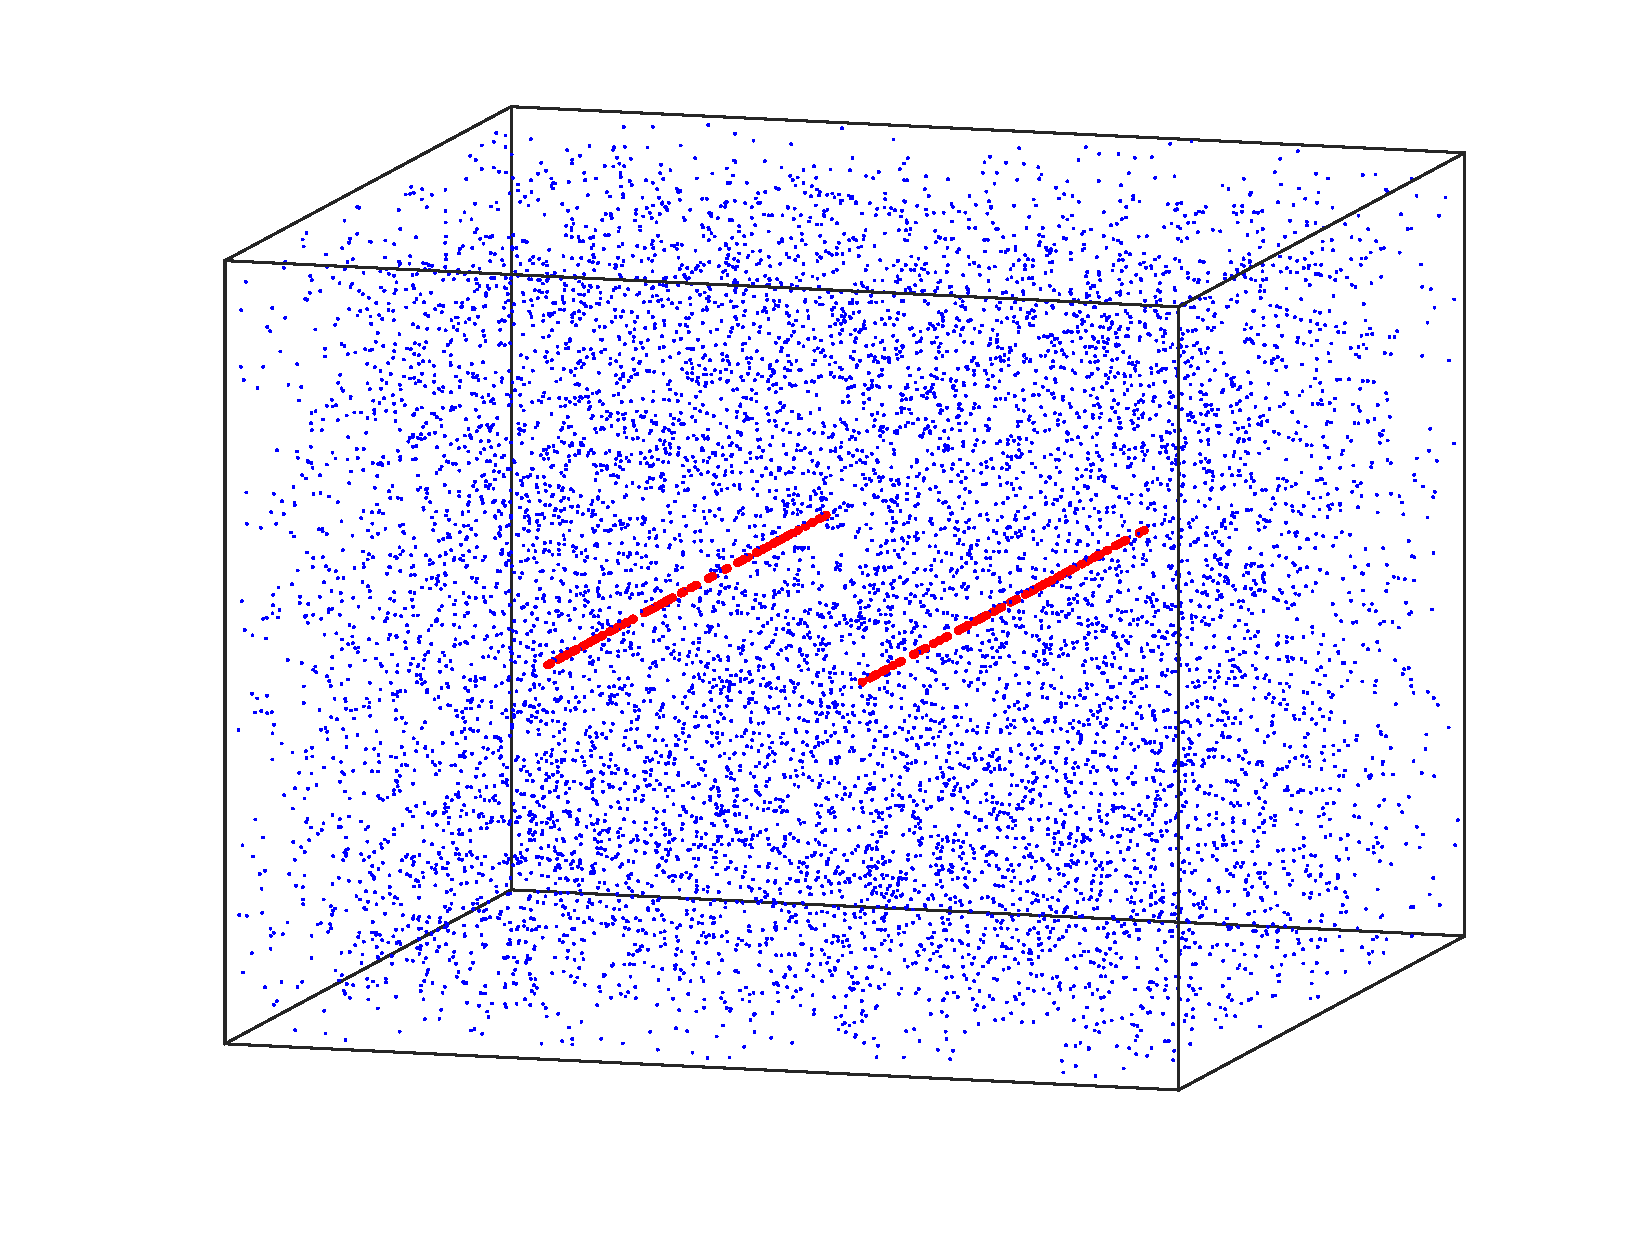
\includegraphics[width=0.8\columnwidth]{gasandwires3.eps}
\\ The double wire system. In blue: bosons. In red: fermions.   
\end{figure}

\newpage

% Chapter 3

\chapter{Induced interaction} % Main chapter title

\label{Chapter3} % For referencing the chapter elsewhere, use \ref{Chapter3} 

\lhead{Part II. \emph{Kitaev wires}}
\chead{Chapter 3. \emph{Induced interaction}} % This is for the header on each page - perhaps a shortened title

%----------------------------------------------------------------------------------------
In this chapter we derive the induced interactions between the fermions on the wires. First stop is to look at the effective interaction between the fermions on the wires and the bosons in the condensate.
\section{Effective Bose-Fermi interaction}
The effective interaction between the fermions ($F$) and the bosons ($B$) is modelled by a delta function potential with strength $g_{BF}$: $V(\mathbf{r})=g_{BF}\delta(\mathbf{r})$. This means, that the \textit{int}eraction Hamiltonian for the effective pair interaction reads:
\begin{equation}
H_{BF}^\text{int}  = \int d^3 r d^3 r' \; \psi_F^\dagger(\mathbf{r}) \psi_B^\dagger(\mathbf{r}')V(\mathbf{r}-\mathbf{r}')\psi_B(\mathbf{r}')\psi_F(\mathbf{r}) = g_{BF}\int d^3 r \; \psi_F^\dagger(\mathbf{r}) \psi_B^\dagger(\mathbf{r})\psi_B(\mathbf{r})\psi_F(\mathbf{r}),
\label{eq.HintBF}
\end{equation}
where $\psi_i(\mathbf{r})$ is the field operator for the $i$-particles, and so $\psi_i^\dagger(\mathbf{r})$ creates a particle at position $\mathbf{r}$.\footnote{The subscript $BF$ specifies, that it is the Hamiltonian for the interaction between bosons and fermions.} Notice, that there is no factor of $1/2$ in front of the integrals. As noted in section \ref{sec.secondquantization} the factor of $1/2$ should be omitted, when the particles are distinguishable, as fermions and bosons most certainly are. 

The fermions ($F$) are confined to two one-dimensional wires. Let the first one be along the $x$-axis, the second at $z = d, y = 0$. The confinement is provided by two harmonic traps in the $y$- and $z$-directions with the same trapping frequency $\omega_t$.\footnote{This is mostly for simplicity. It can easily be generalized to different trapping frequencies $\omega_y$ and $\omega_z$ for the two directions.} In this connection we have two central assumptions. Firstly, we require that the fermions are trapped in the ground state with respect to the perpendicular directions. The energy gap from the ground state to the first excited state is $\omega_t$. Hence by making $\omega_t$ sufficiently large we trap the fermions in the lowest lying state, $\phi_0$, along the two wires. Specifically, the typical energy of the fermions is the free gas Fermi energy $\epsilon_{F,0} = \frac{k_F^2}{2m_F}$. Hence, we require $\frac{\epsilon_{F,0}}{\omega_t} \ll 1$. Using the trapping width $l_t = \frac{1}{\sqrt{m_F\omega_t}}$, we can also express this as $(k_Fl_t)^2 \ll 1$. One might be afraid of violating the Pauli exclusion principle in this context. However, the states in the $x$-direction are allowed to be different, and so we can symmetrize in the $y$- and $z$-directions.

The second assumption is, that the distance between the wires is much larger than the trapping width of the wires, $l_t$. Hence, $l_t/d \ll 1$. This is done, so that we can actually talk about distinguishable wires of fermions. This leads to the following expansion in momentum eigenstates:
\begin{equation}
\psi_F(x,\mathbf{r}_\perp) = \frac{1}{\sqrt{\mathcal{L}}}\sum_p \text{e}^{ipx} \left[\phi_0(\mathbf{r}_\perp) c_{1,p} + \phi_0(\mathbf{r}_\perp - \mathbf{d}) c_{2,p}\right], \hspace{0.5cm} \psi_B(\mathbf{r}) = \frac{1}{\sqrt{\mathcal{V}}}\sum_{\mathbf{k}} \text{e}^{i\mathbf{k}\cdot \mathbf{r}} b_\mathbf{k}, 
\end{equation}  
with $\phi_0(\mathbf{r}_\perp) = \frac{1}{\sqrt{\pi}l_t}\exp\left(-\frac{r_\perp^2}{2l_t^2}\right)$ the harmonic ground state with respect to the perpendicular directions and $\mathbf{d} = d\cdot\hat{z}$ the position of wire 2. $c^\dagger_{j,p}$ creates a fermion in wire $j$ with momentum $p$. $b^\dagger_\mathbf{k}$ creates a boson with momentum $\mathbf{k}$.  We assume, that the wires are truly distinguishable. This means that all anticommutators like $\{c_{1,p}, c^\dagger_{2,p'}\}$ vanish. Inserting these expressions into $H_{BF}^\text{int}$ yields in total four terms. However, the cross terms where a fermion is annihilated in one wire and created in the other are proportional to the integral: $\int d^2 r_\perp \phi_0(\mathbf{r}_\perp)\phi_0(\mathbf{r}_\perp-\mathbf{d}) = 0$. The integral is negligible, because by assumption $l_t/d \ll 1$. The terms arising from interactions with fermions in wire 1 are:
\begin{equation}
H_{BF, 1}^{\text{int}} = \frac{g_{BF}}{\mathcal{LV}}\int d^3 r \sum_{p,p',q,q'}\sum_{\mathbf{k}_{\perp},\mathbf{k}_{\perp}'}\text{e}^{i((p-p')+(q-q'))x} \phi^2_0(\mathbf{r}_{\perp})\text{e}^{i(\mathbf{k}_{\perp} - \mathbf{k}_{\perp}')\cdot \mathbf{r}_\perp} c^\dagger_{1,p'} b^\dagger_{q',\mathbf{k}_\perp'}b_{q,\mathbf{k}_\perp}c_{1,p}. \nonumber
\end{equation}
The integral over $x$ yields the factor $\mathcal{L}\delta_{p-p',q'-q}$, implying total momentum conservation along the wire. The integral over $\mathbf{r}_\perp$ gives the Fourier transform of $\phi_0^2(\mathbf{r}_\perp)$. Since $\phi_0$ is a gaussian, the Fourier transform is as well. Explicitly: $\int d^2 r_\perp \; \phi^2_0(\mathbf{r}_{\perp})\text{e}^{i(\mathbf{k}_{\perp}-\mathbf{k}_{\perp}')\cdot \mathbf{r}_\perp} = \text{e}^{-\frac{l_t^2}{4}(\mathbf{k}_{\perp}-\mathbf{k}_{\perp}')^2}$. Taking the sum over $q'$ forces $q' = p - p' + q$. In total:
\begin{align}
H_{BF, 1}^{\text{int}} &= \frac{g_{BF}}{\mathcal{V}}\sum_{p, p', q} \sum_{\mathbf{k}_\perp, \mathbf{k}_\perp'} \text{e}^{-\frac{l_t^2}{4}(\mathbf{k}_\perp-\mathbf{k}_\perp')^2} c^\dagger_{1, p'} b^\dagger_{p - p' + q, \mathbf{k}_\perp'} b_{q, \mathbf{k}_\perp}c_{1, p} \nonumber \\
                  &= \frac{g_{BF}}{\mathcal{V}}\sum_{p_1, p_2, q} \sum_{\mathbf{k}_\perp, \mathbf{k}_\perp'} \text{e}^{-\frac{l_t^2}{4}(\mathbf{k}_\perp-\mathbf{k}_\perp')^2} c_{1, p_2 - q}^\dagger b_{p_1 + q, \mathbf{k}_\perp'}^\dagger b_{p_1, \mathbf{k}_\perp}c_{1, p_2}.
\end{align}
The last line is obtained by appropriate renaming. To be very specific: $p_1, p_2$ and $q$ are in the $x$ direction, along wire 1, whilst $\mathbf{k}_\perp'$ and $\mathbf{k}_\perp$ are momenta in the $(y,z)$-plane, hence perpendicular to wire 1. The interactions with fermions in wire 2 yields a very similar result. The only alteration is, that $\phi_0(\mathbf{r}_\perp) \to \phi_0(\mathbf{r}_\perp - \mathbf{d})$. The above Fourier transformation therefore yields an additional phase of $\text{e}^{i(\mathbf{k}_\perp - \mathbf{k}_\perp')\cdot \mathbf{d}}$. In total the interaction Hamiltonian hereby becomes:
\begin{align}
H_{BF}^\text{int} = \frac{g_{BF}}{\mathcal{V}}\sum_{p_1,p_2,q} \sum_{\mathbf{k}_\perp, \mathbf{k}_\perp'} & \text{e}^{-\frac{l_t^2}{4}(\mathbf{k}_\perp - \mathbf{k}_\perp')^2}\left[ c^\dagger_{1,p_2-q} b^\dagger_{p_1+q, \mathbf{k}_\perp'} b_{p_1,\mathbf{k}_\perp}c_{1,p_2} + \right. \nonumber \\
& \left. \text{e}^{i(\mathbf{k}_\perp - \mathbf{k}_\perp')\cdot \mathbf{d}}c_{2,p_2-q}^\dagger b_{p_1+q, \mathbf{k}_\perp'}^\dagger b_{p_1,\mathbf{k}_\perp}c_{2,p_2} \right].
\end{align}
This shows, that a scattering event in wire 1 is associated with the factor $g_{BF} \text{e}^{-\frac{l_t^2}{4}(\mathbf{k}_\perp - \mathbf{k}_\perp')^2}$, and that the corresponding scattering in wire 2 has an extra factor of $\text{e}^{i(\mathbf{k}_\perp - \mathbf{k}_\perp')\cdot \mathbf{d}}$. In both cases the transverse momenta are free. An obvious thing to do now would be to take the limit $\omega_t \to \infty$ or equivalently $l_t \to 0$. However, as we shall see later, it will be crucial to keep the trapping frequency finite, at least at the present stage.  

\section{1D-3D induced interactions} \label{sec.1D3Dinducedinteraction}
\subsection{Feynman diagrams} \label{subsec.Feynmandiagrams}
The bosons are assumed to be in a perfect Bose-Einstein condensate (BEC). This means, that they are essentially lying still. We are further only interested in the weak coupling limit.\footnote{There is a small fraction in nonzero momenta states, which is neglected. It would be necessary to include this for a strong interaction.} In a more general setup, one would have to calculate contributions from increasing orders in the underlying bare interaction leading to a socalled $T$-matrix, but this will not be pursued here. We will write the coupling strength as $g_{BF} = \frac{2\pi a_{BF}}{m_r}$, with $m_r = \frac{m_Fm_B}{m_B + m_F}$ the reduced mass, and $a_{BF}$ the effective scattering length. In a formally precise manner one can expand the $T$-matrix in orders of $a_{BF}$. From this analysis, it is clear that the smallness of the coupling strength is equivalent to demanding $(n_Ba_{BF}^3)^{1/3}\ll 1$. We can also argue for this by a dimensional analysis. From the form of $g_{BF}$ it is clear, that we should argue from $a_{BF}$. This has dimension of length, and so we need a parameter of dimension per length to get a unitless expression. The only reasonable parameter is the one that describes how many bosons, the fermions can actually interact with, leading to a length scale $n_B^{-1/3}$. Since a higher density of bosons leads to more fermion-boson interactions, we should therefore assume $(n_Ba_{BF}^3)^{1/3} \ll 1$. In this weak coupling limit we can safely take interactions only up to second order in $g_{BF}$. This means, that the four essential diagrams for the fermion-fermion induced interaction are the ones showed in figure \ref{fig.feynmandiagrams}. 

\begin{figure}
\begin{tikzpicture}[scale=0.25]
  \begin{feynman}[small]
    \vertex (number1) {\( (1) \)};
    \vertex [above left=of number1] (fermion1) {\( \tilde{p}_1 \)};
    \vertex [above right=of fermion1] (a);
    \vertex [below right=of a] (fermion2) {\(\tilde{p}_1 + \tilde{q}\)}; 
    \vertex [above=of a] (b);
    \vertex [left=of b] (boson1) {\( \sqrt{n_B} \)}; 
    \vertex [above= of b] (c);
    \vertex [right= of c] (boson2) {\( \sqrt{n_B} \)};
    \vertex [above= of c] (d);
    \vertex [above left=of d] (f3) {\(\tilde{p}_2\)};
    \vertex [above right=of d] (f4) {\(\tilde{p}_2 - \tilde{q}\)};
 
    \diagram* {
      (number1) -- [opacity=0.0] (fermion1) -- [fermion] (a) -- [fermion] (fermion2),
      (a) -- [photon, edge label'=\(g_{BF}\)] (b),
      (b) -- [dashed] (boson1),
      (b) -- [blue, fermion, edge label' = {\(-\tilde{q}, \mathbf{k}_\perp \)}] (c),
      (c) -- [dashed] (boson2),
      (c) -- [photon, edge label'=\(g_{BF}\)] (d),
      (d) -- [anti fermion] (f3),
      (d) -- [fermion] (f4)
    };
  \end{feynman}
\end{tikzpicture}
\begin{tikzpicture}
  \begin{feynman}[small]
    \vertex (number2) {\( (2) \)};
    \vertex [above left=of number2] (fermion1) {\( \tilde{p}_1 \)};
    \vertex [above right=of fermion1] (a);
    \vertex [below right=of a] (fermion2) {\(\tilde{p}_1 + \tilde{q}\)}; 
    \vertex [above=of a] (b);
    \vertex [left=of b] (boson1) {\( \sqrt{n_B} \)}; 
    \vertex [above= of b] (c);
    \vertex [right= of c] (boson2) {\( \sqrt{n_B} \)};
    \vertex [above= of c] (d);
    \vertex [above left=of d] (f3) {\(\tilde{p}_2\)};
    \vertex [above right=of d] (f4) {\(\tilde{p}_2 - \tilde{q}\)};
 
    \diagram* {
      (number2) -- [opacity=0.0] (fermion1) -- [fermion] (a) -- [fermion] (fermion2),
      (a) -- [photon, edge label'=\(g_{BF}\)] (b),
      (b) -- [dashed] (boson1),
      (b) -- [blue, anti fermion, edge label' = {\(\tilde{q}, \mathbf{k}_\perp \)}] (c),
      (c) -- [dashed] (boson2),
      (c) -- [photon, edge label'=\(g_{BF}\)] (d),
      (d) -- [anti fermion] (f3),
      (d) -- [fermion] (f4)
    };
  \end{feynman}
\end{tikzpicture}
\begin{tikzpicture}
  \begin{feynman}[small]
    \vertex (number3) {\( (3) \)};
    \vertex [above left=of number3] (fermion1) {\( \tilde{p}_1 \)};
    \vertex [above right=of fermion1] (a);
    \vertex [below right=of a] (fermion2) {\(\tilde{p}_1+\tilde{q}\)}; 
    \vertex [above=of a] (b);
    \vertex [left=of b] (boson1) {\( \sqrt{n_B} \)}; 
    \vertex [above= of b] (c);
    \vertex [right= of c] (boson2) {\( \sqrt{n_B} \)};
    \vertex [above= of c] (d);
    \vertex [above left=of d] (f3) {\(\tilde{p}_2\)};
    \vertex [above right=of d] (f4) {\(\tilde{p}_2-\tilde{q}\)};
 
    \diagram* {
      (number3) -- [opacity=0.0] (fermion1) -- [fermion] (a) -- [fermion] (fermion2),
      (a) -- [photon, edge label'=\(g_{BF}\)] (b),
      (b) -- [dashed] (boson1),
      (b) -- [blue, majorana, edge label' = {\(\tilde{q}, \mathbf{k}_\perp \)}] (c),
      (c) -- [dashed] (boson2),
      (c) -- [photon, edge label'=\(g_{BF}\)] (d),
      (d) -- [anti fermion] (f3),
      (d) -- [fermion] (f4)
    };
  \end{feynman}
\end{tikzpicture}
\begin{tikzpicture}
  \begin{feynman}[small]
    \vertex (number4) {\( (4) \)};
    \vertex [above left=of number4] (fermion1) {\( \tilde{p}_1 \)};
    \vertex [above right=of fermion1] (a);
    \vertex [below right=of a] (fermion2) {\(\tilde{p}_1+\tilde{q}\)}; 
    \vertex [above=of a] (b);
    \vertex [left=of b] (boson1) {\( \sqrt{n_B} \)}; 
    \vertex [above= of b] (c);
    \vertex [right= of c] (boson2) {\( \sqrt{n_B} \)};
    \vertex [above= of c] (d);
    \vertex [above left=of d] (f3) {\(\tilde{p}_2\)};
    \vertex [above right=of d] (f4) {\(\tilde{p}_2-\tilde{q}\)};
 
    \diagram* {
      (number3) -- [opacity=0.0] (fermion1) -- [fermion] (a) -- [fermion] (fermion2),
      (a) -- [photon, edge label'=\(g_{BF}\)] (b),
      (b) -- [dashed] (boson1),
      (b) -- [blue, anti majorana, edge label' = {\(\tilde{q}, \mathbf{k}_\perp \)}] (c),
      (c) -- [dashed] (boson2),
      (c) -- [photon, edge label'=\(g_{BF}\)] (d),
      (d) -- [anti fermion] (f3),
      (d) -- [fermion] (f4)
    };
  \end{feynman}
\end{tikzpicture}
\caption{Feynman diagrams for the induced interaction. Since the interaction is weak, we can neglect all other Feynman diagrams than (1)-(4). Diagrams (1) and (2) stems from the normal Green's function $G_{11}$. Diagrams (3) and (4) stems from the anormalous Green's functions $G_{12}$ and $G_{21}$. The diagrams have the exact same form for interactions between fermions in the same and opposite wires. The only difference is, that $g_{BF}$ carries an extra phase factor for interactions in wire 2. } 
\label{fig.feynmandiagrams}
\end{figure}

Notice that the bosons of the BEC, shown with dashed lines, carry a factor of $\sqrt{n_B}$. This is simply because it is the pour condensate wave function. Further $\tilde{p}_j = (p_j, i\omega_{m_j})$, with $\omega_{m} = (2m + 1)\pi kT$ a fermionic Matsubara frequency, and $\tilde{q} = (q, i\omega_q )$, with $\omega_q = \omega_{m_1} - \omega_{m_2}$ a bosonic Matsubara frequency. The blue lines in the diagrams are the normal and anormalous Bogoliubov phonon Green's functions derived in subsection \ref{sec.BECGreens}. Functionally they are:
\begin{equation}
G_{11}(\mathbf{k},i\omega_m) = \frac{u_{B,k}^2}{i\omega_m-E_{B,k}}-\frac{v_{B,k}^2}{i\omega_m+E_{B,k}}, \hspace{0.5cm} G_{12}(\mathbf{k},i\omega_m) = G_{21}(\mathbf{k},i\omega_m) = \frac{u_{B,k}v_{B,k}}{i\omega_m+E_{B,k}}-\frac{u_{B,k}v_{B,k}}{i\omega_m-E_{B,k}}.\nonumber
\end{equation}
Here $u_{B,k}$ and $v_{B,k}$ are the BEC coherence factors found in subsection \ref{sec.BEC} with $m_B$ the mass of the bosons. Further $\xi_{B,k} = \frac{k^2}{2m_B} + n_Bg_B$ and $g_B = \frac{4\pi a_B}{m_B}$, with $a_B$ the scattering length in the BEC. Finally $E_{B,k}^2 = \xi_{B,k}^2-(n_Bg_B)^2$ is the BEC Bogoliubov spectrum.

The diagrams can intuitively be understood as follows. A fermion in one wire interact with a (real) boson in the condensate. This creates a ripple in the condensate described by one of the Green's functions. This ripple reaches a second fermion in one of the two wires, where the momentum of the ripple is transferred to. Further, a (real) boson is "returned" to the condensate. In a more technical way we say, that the fermions interact by exchanging a condensate Bogoliubov phonon. 

Let us first focus on the induced interaction of two fermions in wire 1. Since the perpendicular momentum $\mathbf{k}_\perp$ is completely free we have to integrate over this. Since the momentum of the incoming and outgoing boson in each diagram is 0 we simply get a factor of $g_{BF}\; \text{e}^{-\frac{l_t^2}{4}k_\perp^2}$ \textit{twice}. Collecting all terms gives us the four contributions from the four diagrams (1)-(4) to the fermion-fermion induced interaction $V_{\text{ind}}$: 
\begin{align}
V^{11}_{\text{ind}, 1}(q,i\omega_q) &= n_Bg_{BF}^2\int\frac{d^2k_\perp}{(2\pi)^2}G_{11}(-q,\mathbf{k}_\perp,-\omega_q)\text{e}^{-\frac{l_t^2}{2}k_\perp^2}, \nonumber \\
V^{11}_{\text{ind}, 2}(q,i\omega_q) &= n_Bg_{BF}^2\int\frac{d^2k_\perp}{(2\pi)^2}G_{11}(q,\mathbf{k}_\perp,\omega_q)\text{e}^{-\frac{l_t^2}{2}k_\perp^2}, \nonumber \\
V^{11}_{\text{ind}, 3}(q,i\omega_q) &= n_Bg_{BF}^2\int\frac{d^2k_\perp}{(2\pi)^2}G_{12}(q,\mathbf{k}_\perp,\omega_q)\text{e}^{-\frac{l_t^2}{2}k_\perp^2}, \nonumber \\
V^{11}_{\text{ind}, 4}(q,i\omega_q) &= n_Bg_{BF}^2\int\frac{d^2k_\perp}{(2\pi)^2}G_{12}(q,\mathbf{k}_\perp,\omega_q)\text{e}^{-\frac{l_t^2}{2}k_\perp^2}. 
\end{align}
We notice, that the last two give the same contribution in this weak interacting limit.\footnote{This would \textit{not} be the case, when including higher order terms.} The 11 superscript means, that it is for two fermions in wire 1. Summing up the four contributions gives us the frequency dependent induced interaction $V^{11}_{\text{ind}}$ for fermions in wire 1:
\begin{equation}
V^{11}_{\text{ind}}(q,i\omega_q) = g_{BF}^2\int\frac{d^2k_\perp}{(2\pi)^2}\; \chi_\text{BEC}(q,\mathbf{k}_\perp,i\omega_q)\text{e}^{-\frac{l_t^2}{2}k_\perp^2}, 
\label{eq.V11indXBEC}
\end{equation}
with $\chi_\text{BEC}(\mathbf{k},i\omega_q) = \frac{k^2}{m_B}\frac{n_B}{(i\omega_q)^2 - E_{B,k}^2}$ the socalled density-density correlation function of the BEC. It now becomes clear, why we had to retain a nonzero value of $l_t$ at this stage. For $l_t\to 0$ the above has an integrand of the form $k^2/(a + bk^4 + ck^2)$, with $a,b,c$ positive constants. As a result the integral is logarithmically divergent. The situation in a 2D-3D system is different. Here there is a single integral in the above, and the result converges for $l_t\to 0$. We return to this later on. Intuitively, the induced interaction of fermions in wire 2 must be the same as the above. However, one might wonder what happens to the extra factor of $\text{e}^{i(\mathbf{k}_\perp - \mathbf{k}_\perp')\cdot \mathbf{d}}$ for wire 2. The incoming boson is associated with a factor of $\text{e}^{i\mathbf{k}_\perp\cdot \mathbf{d}}$. However, the outgoing is associated with a factor of $\text{e}^{-i\mathbf{k}_\perp\cdot \mathbf{d}}$, and so these cancel. Hence, we have $V^{22}_{\text{ind}}(q,i\omega_q) = V^{11}_{\text{ind}}(q,i\omega_q)$. These interactions we denote \textit{intra}wire interactions. 

Additionally, there is an \textit{inter}wire induced interaction between the wires, which we will denote $V_{\text{ind}}^{12}(q,i\omega_q)$. The preceding section shows, that the calculation of this induced interaction is analogous to the above, but with the additional factor of $\text{e}^{i\mathbf{k}_\perp\cdot \mathbf{d}}$ from scattering in the second wire. Hence:
\begin{equation}
V_{\text{ind}}^{12}(q,i\omega_q) = g_{BF}^2\int\frac{d^2k_\perp}{(2\pi)^2}\; \chi_\text{BEC}(q,\mathbf{k}_\perp, i\omega_q)\text{e}^{-\frac{l_t^2}{2}k_\perp^2}\text{e}^{i\mathbf{k}_\perp\cdot \mathbf{d}}. 
\label{eq.V12indXBEC} 
\end{equation}
We notice, that the \textit{inter}wire interaction goes to the \textit{intra}wire interaction for $d \to 0$. It turns out, that we can find quite simple expressions for the induced interaction in real space in the zero frequency limit: $\omega_q = 0$. Since we in general are going to restrict ourselves to this limit, we briefly discuss, what it physically means. 

\subsection{Retardation effects} \label{sec.RetardationEffects}
From equations \eqref{eq.V11indXBEC} and \eqref{eq.V12indXBEC} it is evident that the induced interactions have a frequency dependency. This dependency reflects, that the fermions do not interact instanteneously, socalled retardation effects. In turn this embodies, that the phonons in the condensate, the mediators of the fermion-fermion interaction, moves at a finite speed $c_0 = \sqrt{\frac{n_Bg_B}{m_B}} = \frac{\sqrt{4\pi n_B a_B}}{m_B}$.\footnote{It is analogous to the retarded fields in electrodynamics. There it reflects the finiteness of the speed of light.} To neglect these effects we therefore need to assume, that the typical speed of the fermions is much smaller than the speed of the bosons: $v_F \ll c_0$, $v_F = k_F/m_F$ the Fermi speed for free fermions. This leads to the relation:
\begin{equation}
1 \gg \frac{v_F}{c_0} = \frac{\sqrt{\pi}}{2} \frac{m_B}{m_F}\frac{1}{ \sqrt{ (n_Ba_B^3)^{1/3} } }\frac{n_F}{ n_B^{1/3} } = \frac{m_B}{m_F}\frac{k_F\xi}{\sqrt{2}}, 
\label{eq.RetardationEffectsneglectionassumption}
\end{equation}
whereby we have expressed the ratio of velocities in terms of unitless quantities and in terms of the coherence length, $\xi$, defined by $\frac{1}{\xi^2} = 2m_Bn_Bg_B$. With this assumption at hand we can focus on the zero frequency induced interaction $V^{ij}_{\text{ind}}(q,0)$. For fermions and bosons of similar mass we notice, that the neglect of retardation effects is equivalent to only studying short range interactions: $k_F\xi \lesssim 1$. 

\subsection{Real space}
\label{subsec.inducedinteraction.realspace}
In this subsection we calculate the real space interactions, $\tilde{V}^{ij}_{\text{ind}}(x, 0)$. 

We start with the \textit{inter}wire interaction. We get:
\begin{equation}
V^{12}_{\text{ind}}(x, 0) = \int \frac{dq}{2\pi} \; \text{e}^{iqx} V^{12}_{\text{ind}}(q, 0) = g^2_{BF}\int \frac{d^3 k}{(2\pi)^3}\;\chi_\text{BEC}(\mathbf{k}, 0)\text{e}^{-\frac{l_t^2}{2}k_\perp^2}\text{e}^{i\mathbf{k}\cdot \mathbf{r}}, \nonumber
\end{equation}
where we write $\mathbf{k} = (q, \mathbf{k}_{\perp})$ and $\mathbf{r} = (x, \mathbf{r}_{\perp})$. The above expression converges for $l_t \to 0$, because the integrand is monotonically increasing for decreasing $l_t$. The gaussian, $\text{e}^{-\frac{l_t^2}{2}k_\perp^2}$, hereby drops out and we are left with the Fourier transformation of $\chi_\text{BEC}(\mathbf{k}, 0) = -4m_Bn_B\frac{1}{k^2 + 1/\xi^2}$. We recognise this as the Yukawa potential in momentum space. For completeness we here show how to perform the Fourier transformation. The integral of interest is:
\begin{equation}
I(\mathbf{r}) = \int \frac{d^3 k}{(2\pi)^3} \frac{1}{k^2 + 1/\xi^2}\text{e}^{i\mathbf{k}\cdot\mathbf{r}} = \int_{0}^{\pi}d\theta \sin(\theta)\int_{0}^{\infty}\frac{dk}{(2\pi)^2} \frac{k^2}{k^2 + 1/\xi^2}\text{e}^{ikr\cos(\theta)},
\label{eq.def.Fourierintegral}
\end{equation}
where we in the second expression set the angle between $\mathbf{k}$ and $\mathbf{r}$ to be $\theta$ and transform the integral to polar coordinates. We have further used, that the integrand does not depend on the azimuthal angle, $\phi$, so that this integral simple yields a factor of $2\pi$. The $\theta$ dependent part then simply gives:
\begin{equation}
\int_{0}^{\pi}d\theta \sin(\theta)\text{e}^{ikr\cos(\theta)} = -\left.\frac{1}{ikr}\text{e}^{ikr\cos(\theta)}\right|_{0}^{\pi} = \frac{1}{ikr}\left(\text{e}^{ikr} - \text{e}^{-ikr}\right). \nonumber
\end{equation}
Inserting this into equation \eqref{eq.def.Fourierintegral} yields: $I(\mathbf{r}) = \frac{1}{2\pi r}\int \frac{dk}{2\pi i} \frac{k}{k^2 + 1/\xi^2}\text{e}^{ikr}$, where the integration limits are now implicitly $\pm \infty$. This integral is solvable using Cauchy's residue theorem. Explicitly, we now think of $k$ as a complex variable. We define the half-circle contour $\mathcal{C}$ in the upper half-plane with a radius $R$ tending to infinity. Since $r > 0$ the integrand goes exponentially to zero at the circle boundary, so that this part of the contour integral does not contribute. We have to find the poles of the integrand in the upper complex plane of $k$ and calculate the residues. There is a single pole given by $k = \frac{i\sqrt{2}}{\xi}$. Cauchy's residue theorem then states, that:
\begin{equation}
I(\mathbf{r}) = \frac{1}{2\pi r}\int \frac{dk}{2\pi i} \frac{k}{k^2 + 1/\xi^2}\text{e}^{ikr} = \frac{1}{2\pi r}\text{Res}\left(\frac{k}{k^2 + 1/\xi^2}\text{e}^{ikr}, \frac{i\sqrt{2}}{\xi}\right) = \frac{1}{4\pi r} \text{e}^{-\sqrt{2}r/\xi}, \nonumber
\end{equation}
where $\text{Res}(f(x), x_0)$ denotes the residue of $f(x)$ in $x = x_0$. Setting $\mathbf{r} = (x, \mathbf{d})$ we get for the induced interaction between the wires:
\begin{equation}
V^{12}_{\text{ind}}(x, 0) = -4m_Bg^2_{BF}n_B I(x, \mathbf{d}) = -\frac{m_Bg_{BF}^2n_B}{\pi}\frac{\text{e}^{ -\sqrt{2}\sqrt{x^2 + d^2}/\xi }}{\sqrt{x^2 + d^2}}.
\label{eq.V12indx}
\end{equation}
As noted in section \ref{sec.1D3Dinducedinteraction} we can obtain the intrawire interaction by simply setting $d = 0$. We get:
\begin{equation}
V^{11}_{\text{ind}}(x, 0) = -\frac{m_Bg_{BF}^2n_B}{\pi}\frac{\text{e}^{ -\sqrt{2}|x|/\xi }}{|x|}.
\label{eq.V11indx}
\end{equation}
The induced interaction in real space is seen to be the Yukawa interaction with a range of interaction given by the BEC coherence length, $\xi$. We can also understand this physically. The coherence length is in general the length scale over which, the condensate adjusts to an influence on the boson density. Hence, it is physically intuitive that this is exactly the range of the interaction. 

We could also have calculated the intrawire induced interaction for a general $l_t > 0$ and then taken the $l_t \to 0$ limit. The reader is referred to appendix \ref{Appendix.intrawireinteraction.ltnonzero} to see this explicitly. In the end it gives the same result. 

We get a unitless form of the real space interaction by dividing with the typical energy of the fermions, the Fermi energy $\epsilon_{F,0}$. In this way the resulting front factor of $V^{11}_{\text{ind}} / \epsilon_{F,0}$ is a measure of the strength of interaction given by:
\begin{equation}
G = - 8\left( \frac{m_F}{m_B} + \frac{m_B}{m_F} + 2 \right) \frac{n_B^{1/3}}{n_F}(n_Ba_{BF}^3)^{2/3}.
\label{eq.interactionstrength.wires}
\end{equation}
The mass ratio $m_B / m_F$, The relative interparticle distance $n_B^{1/3} / n_F$ and the Bose-Fermi gas parameter $(n_Ba_{BF}^3)^{1/3}$ hereby comes naturally about by going to unitless quantities. 

In figure \ref{fig.V11indx} we show, how the Yukawa interaction for the intrawire case is approached in the $l_t\to 0$ limit. In figure \ref{fig.V12indx} we show the interwire interaction for several interwire distances, $d$. 

\begin{figure} 
\begin{center}  
\input{Figures/Vx/plot.tex}  
\caption{The zero frequency \textit{intra}wire interaction $\tilde{V}^{11}_{\text{ind}}(x,0)$ plotted as a function of $k_Fx$ for several values of $l_t$. The black curve is the asymptotic Yukawa interaction for $l_t \to 0$. Parameters: $(n_Ba_B^3)^{1/3} = 0.01$, $(n_Ba_{BF}^3)^{1/3} = 0.1$, $\frac{m_B}{m_F} = 7/40$, $\frac{n_F}{n_B^{1/3}} = 0.215$, $v_F/c_0 = 0.33$.}  
\label{fig.V11indx}  
\vspace{0.5cm}
% GNUPLOT: LaTeX picture with Postscript
\begingroup
  \makeatletter
  \providecommand\color[2][]{%
    \GenericError{(gnuplot) \space\space\space\@spaces}{%
      Package color not loaded in conjunction with
      terminal option `colourtext'%
    }{See the gnuplot documentation for explanation.%
    }{Either use 'blacktext' in gnuplot or load the package
      color.sty in LaTeX.}%
    \renewcommand\color[2][]{}%
  }%
  \providecommand\includegraphics[2][]{%
    \GenericError{(gnuplot) \space\space\space\@spaces}{%
      Package graphicx or graphics not loaded%
    }{See the gnuplot documentation for explanation.%
    }{The gnuplot epslatex terminal needs graphicx.sty or graphics.sty.}%
    \renewcommand\includegraphics[2][]{}%
  }%
  \providecommand\rotatebox[2]{#2}%
  \@ifundefined{ifGPcolor}{%
    \newif\ifGPcolor
    \GPcolortrue
  }{}%
  \@ifundefined{ifGPblacktext}{%
    \newif\ifGPblacktext
    \GPblacktexttrue
  }{}%
  % define a \g@addto@macro without @ in the name:
  \let\gplgaddtomacro\g@addto@macro
  % define empty templates for all commands taking text:
  \gdef\gplbacktext{}%
  \gdef\gplfronttext{}%
  \makeatother
  \ifGPblacktext
    % no textcolor at all
    \def\colorrgb#1{}%
    \def\colorgray#1{}%
  \else
    % gray or color?
    \ifGPcolor
      \def\colorrgb#1{\color[rgb]{#1}}%
      \def\colorgray#1{\color[gray]{#1}}%
      \expandafter\def\csname LTw\endcsname{\color{white}}%
      \expandafter\def\csname LTb\endcsname{\color{black}}%
      \expandafter\def\csname LTa\endcsname{\color{black}}%
      \expandafter\def\csname LT0\endcsname{\color[rgb]{1,0,0}}%
      \expandafter\def\csname LT1\endcsname{\color[rgb]{0,1,0}}%
      \expandafter\def\csname LT2\endcsname{\color[rgb]{0,0,1}}%
      \expandafter\def\csname LT3\endcsname{\color[rgb]{1,0,1}}%
      \expandafter\def\csname LT4\endcsname{\color[rgb]{0,1,1}}%
      \expandafter\def\csname LT5\endcsname{\color[rgb]{1,1,0}}%
      \expandafter\def\csname LT6\endcsname{\color[rgb]{0,0,0}}%
      \expandafter\def\csname LT7\endcsname{\color[rgb]{1,0.3,0}}%
      \expandafter\def\csname LT8\endcsname{\color[rgb]{0.5,0.5,0.5}}%
    \else
      % gray
      \def\colorrgb#1{\color{black}}%
      \def\colorgray#1{\color[gray]{#1}}%
      \expandafter\def\csname LTw\endcsname{\color{white}}%
      \expandafter\def\csname LTb\endcsname{\color{black}}%
      \expandafter\def\csname LTa\endcsname{\color{black}}%
      \expandafter\def\csname LT0\endcsname{\color{black}}%
      \expandafter\def\csname LT1\endcsname{\color{black}}%
      \expandafter\def\csname LT2\endcsname{\color{black}}%
      \expandafter\def\csname LT3\endcsname{\color{black}}%
      \expandafter\def\csname LT4\endcsname{\color{black}}%
      \expandafter\def\csname LT5\endcsname{\color{black}}%
      \expandafter\def\csname LT6\endcsname{\color{black}}%
      \expandafter\def\csname LT7\endcsname{\color{black}}%
      \expandafter\def\csname LT8\endcsname{\color{black}}%
    \fi
  \fi
    \setlength{\unitlength}{0.0500bp}%
    \ifx\gptboxheight\undefined%
      \newlength{\gptboxheight}%
      \newlength{\gptboxwidth}%
      \newsavebox{\gptboxtext}%
    \fi%
    \setlength{\fboxrule}{0.5pt}%
    \setlength{\fboxsep}{1pt}%
\begin{picture}(7200.00,5040.00)%
    \gplgaddtomacro\gplbacktext{%
      \csname LTb\endcsname%
      \put(946,767){\makebox(0,0)[r]{\strut{}$-3$}}%
      \csname LTb\endcsname%
      \put(946,1469){\makebox(0,0)[r]{\strut{}$-2.5$}}%
      \csname LTb\endcsname%
      \put(946,2170){\makebox(0,0)[r]{\strut{}$-2$}}%
      \csname LTb\endcsname%
      \put(946,2872){\makebox(0,0)[r]{\strut{}$-1.5$}}%
      \csname LTb\endcsname%
      \put(946,3573){\makebox(0,0)[r]{\strut{}$-1$}}%
      \csname LTb\endcsname%
      \put(946,4275){\makebox(0,0)[r]{\strut{}$-0.5$}}%
      \csname LTb\endcsname%
      \put(946,4976){\makebox(0,0)[r]{\strut{}$0$}}%
      \csname LTb\endcsname%
      \put(1701,484){\makebox(0,0){\strut{}$-4$}}%
      \csname LTb\endcsname%
      \put(2821,484){\makebox(0,0){\strut{}$-2$}}%
      \csname LTb\endcsname%
      \put(3941,484){\makebox(0,0){\strut{}$0$}}%
      \csname LTb\endcsname%
      \put(5060,484){\makebox(0,0){\strut{}$2$}}%
      \csname LTb\endcsname%
      \put(6180,484){\makebox(0,0){\strut{}$4$}}%
    }%
    \gplgaddtomacro\gplfronttext{%
      \csname LTb\endcsname%
      \put(176,2871){\rotatebox{-270}{\makebox(0,0){\strut{}$V_{FF,12}^\text{ind}(x,0)/\epsilon_{F,0}$}}}%
      \put(3940,154){\makebox(0,0){\strut{}$k_Fx$}}%
      \csname LTb\endcsname%
      \put(2461,1600){\makebox(0,0)[r]{\strut{}$k_Fd = 1.8$}}%
      \csname LTb\endcsname%
      \put(2461,1380){\makebox(0,0)[r]{\strut{}$k_Fd = 1.4$}}%
      \csname LTb\endcsname%
      \put(2461,1160){\makebox(0,0)[r]{\strut{}$k_Fd = 1.0$}}%
      \csname LTb\endcsname%
      \put(2461,940){\makebox(0,0)[r]{\strut{}$k_Fd = 0.6$}}%
    }%
    \gplbacktext
    \put(0,0){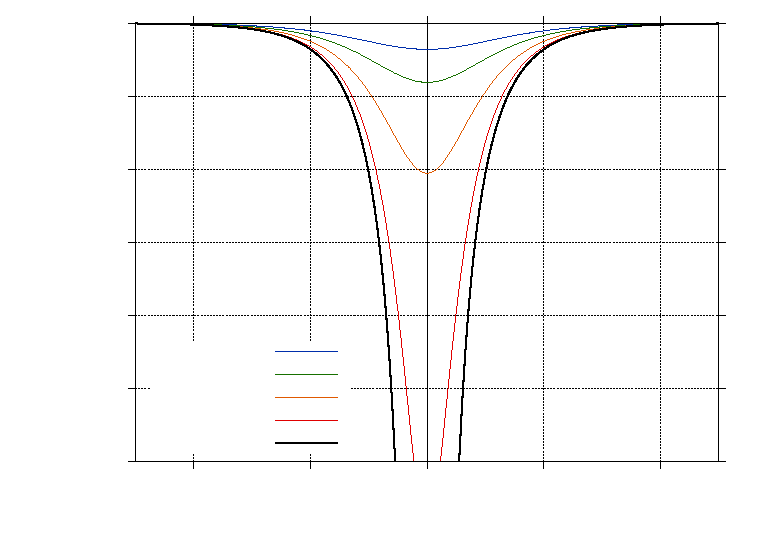
\includegraphics{Figures/twowires/InducedInteractionInterwireRealSpace/InducedInteraction}}%
    \gplfronttext
  \end{picture}%
\endgroup
  
\caption{The zero frequency \textit{inter}wire interaction $\tilde{V}_{\text{ind}}^{12}(x,0)$ plotted as a function of $x$. The induced interaction is seen to increase with decreasing distance $d$. Parameters: $(n_Ba_B^3)^{1/3} = 0.01$, $(n_Ba_{BF}^3)^{1/3} = 0.1$, $l_t = 0$, $\frac{m_B}{m_F} = 7/40$, $\frac{n_F}{n_B^{1/3}} = 0.215$, $v_F/c_0 = 0.33$.}  
\label{fig.V12indx}  
\end{center}    
\end{figure}

In appendix \ref{Appendix.inducedinteraction.realspace} we calculate the real space induced interaction for general Matsubara frequencies $\omega_m = 2\pi m k_BT$ in the $l_t = 0$ limit. This general interaction is qualitatively the same as the zero frequency component.  

\subsection{Momentum space}
\label{subsec.inducedinteraction.momentumspace}
In this section we calculate the momentum space induced interactions.

We start with the \textit{inter}wire interaction. In chapter \ref{Chapter4} we will see, that the relevant expression is simply the Fourier transform of the real space interaction. Therefore, we could go back to equation \eqref{eq.V12indXBEC} for $\omega_q = 0$. However, it is simpler to use the real space expression found in subsection \ref{subsec.inducedinteraction.realspace} and perform the Fourier transform explicitly. We get:
\begin{equation}
V_{\text{ind}}^{12}(q,0) = \int dx \; \text{e}^{-iqx}\tilde{V}_{\text{ind}}^{12}(x,0) = 2\int_0^\infty \cos(qx)\tilde{V}_{\text{ind}}^{12}(x,0), \nonumber
\end{equation}
since the induced interaction is even in real space. Writing the variables in units of the range $\xi/\sqrt{2}$:
\begin{equation}
V_{\text{ind}}^{12}(\tilde{q},0) = -\frac{2n_Bg^2_{BF}m_B}{\pi}\int_0^\infty d\tilde{x} \cos(\tilde{q}\tilde{x})\frac{ \text{e}^{ -\sqrt{\tilde{x}^2+\tilde{d}^2} } }{\sqrt{\tilde{x}^2+\tilde{d}^2}} = -\frac{2n_Bg^2_{BF}m_B}{\pi}K_0\left[\tilde{d}\sqrt{\tilde{q}^2+1}\right], \nonumber
\end{equation}
where $K_0(x)$ is the modified Bessel function of the second kind of order zero. This calculation is done with the use of the Fourier cosine transform routine in Maple 16. Since $\tilde{q} = \frac{q\xi}{\sqrt{2}}, \tilde{d} = \frac{\sqrt{2}d}{\xi}$, we finally get:
 \begin{equation}
V_{\text{ind}}^{12}(q,0) = -\frac{2n_Bg^2_{BF}m_B}{\pi}K_0\left[\sqrt{(qd)^2+\frac{2d^2}{\xi^2}}\right]. 
\label{eq.V12indq.zerofrequency}
\end{equation}
We hereby have a closed form expression for the interwire induced interaction in momentum space. 

Next we turn to the \textit{intra}wire interaction. The situation here is more tricky. As already noted, the induced interaction in equation \eqref{eq.V11indXBEC} diverges for $l_t \to 0$. However, in chapter \ref{Chapter4} we will see, that the anticommutator relations for the fermionic creation and annihilation operators leads to the following expression for the scattering amplitude in momentum space:
\begin{equation}
W^{11}_{\text{ind}}(k, q, p) = \frac{1}{2}\left(V^{11}_{\text{ind}}\left( p, 0 \right) - V^{11}_\text{ind}\left( p + k - q, 0 \right) \right). 
\label{eq.Wkqp.scattering.amplitude}
\end{equation}
The scattering amplitude is hereby a combination of two Fourier transforms. We will comment further on the meaning of this expression in chapter \ref{Chapter4}. For now we simply wish to calculate the $l_t \to 0$ limit. Going back to equation \eqref{eq.V11indXBEC} for $\omega_q = 0$, it turns out, that we can express $V_\text{ind}\left( q, 0 \right)$ as:
\begin{equation}
V^{11}_{\text{ind}}(q, 0) = -\frac{m_Bg_{BF}^2n_B}{\pi} \text{e}^{F(q)} E_1(F(q)),
\label{eq.V11indq.zerofrequency.ltnonzero}
\end{equation}
where $F(q) = \frac{l_t^2}{2}\left(q^2 + \frac{2}{\xi^2} \right)$ and $E_1(x)$ is the exponential integral: $E_1(x) = \int_1^\infty du \frac{\text{e}^{-xu}}{u}$. Inserting this into the above expression for $W^{11}_{\text{ind}}$ yields:
\begin{align}
W^{11}_{\text{ind}}(k, q, p) &= \frac{1}{2}\left[V^{11}_\text{ind}(p, 0) - V^{11}_\text{ind}(p + k - q, 0)\right] \nonumber \\
&= -\frac{m_Bg_{BF}^2n_B}{2\pi}\left[ \text{e}^{F(p)} E_1(F(p)) - \text{e}^{F(p + k - q)} E_1(F(p + k - q)) \right], \nonumber
\end{align}
Now we take the $l_t \to 0$ limit. We have $\partial_x E_1(x) = -\int_1^{\infty}du\; \text{e}^{-xu} = -\frac{1}{x}\text{e}^{-x}$. For $0 < x \ll 1$, this gives $\partial_xE_1(x) = -\frac{1}{x}$. Hence, in this regime we have $E_1(x) = C -\ln(x)$, where $C$ is a constant.\footnote{The constant is minus the Euler-Mascheroni constant $\gamma$. To ten digits precision $\gamma = 0.5772156649$. This is found in Maple 16.} The exponentials $\text{e}^{F(p)}$ and $\text{e}^{F(k + p - q)}$ just give $1$ in the $l_t \to 0$ limit, and so we are left with the expression:
\begin{equation}
\lim_{l_t \to 0} \; W^{11}_{\text{ind}}(k, q, p) = -\frac{m_Bg_{BF}^2n_B}{2\pi} \ln\left[\frac{(k - q + p)^2 + 2/\xi^2}{p^2 + 2/\xi^2}\right].
\label{eq.Wkqp.scattering.amplitude.lt=0} 
\end{equation}
Hereby we also have a closed form expression for the intrawire interaction in momentum space. The fact that we have these closed form expressions is crucial for the feasibility of the later numerical analyses.





% Chapter 4

\chapter{Grand Fermi Hamiltonian} % Main chapter title

\label{Chapter4} % For referencing the chapter elsewhere, use \ref{Chapter3} 

\lhead{Part II. \emph{One wire}}
\chead{Chapter 4. \emph{Grand Fermi Hamiltonian}} % This is for the header on each page - perhaps a shortened title

%----------------------------------------------------------------------------------------
In this chapter we will study the induced interactions more extensively. Firstly, we calculate the pair interaction Hamiltonian for the fermions in section \ref{sec.HFFint}. This is done under the assumption, that we can restrict the induced interactions to have a vanishing Matsubara frequency: $\omega_q = 0$. See subsection \ref{sec.RetardationEffects} for details. The result for the interaction Hamiltonian is then inserted into the full Hamiltonian in section \ref{sec.HFFfull}. The approach is an example of a Bardeen-Cooper-Schrieffer (BCS) theory, see e.g. \cite[chapter 3]{Tinkham}, \cite[pp. 153-163]{LandauStatPhys2} and \cite[pp. 359-369]{PlischkeStatPhys}. 

\section{Interaction Hamiltonian} \label{sec.HFFint}
In this section we transform the interactions from real to momentum space. The \textit{intrawire} interaction Hamiltonian for pair interactions between fermions in wire 1 is given by:
\begin{equation}
H^\text{int,11}_{FF} = \frac{1}{2}\int dx_1dx_2\; \psi^\dagger_{1,F}(x_1)\psi^\dagger_{1,F}(x_2)\tilde{V}^{11}_{\text{ind}}(x_1 - x_2, 0) \psi_{1,F}(x_2) \psi_{1,F}(x_1).
\label{eq.HFF11intdef}
\end{equation}
With $\tilde{V}^{11}_\text{ind}(x,0)$ the induced interaction at zero frequency in real space, equation \eqref{eq.V11indx}. The factor of $1/2$ is present, since the particles are identical. Transforming the above expression to momentum space will make it clearer of how to perform the BCS assumption and in turn the mean field approximation. 

The transformation to momentum space is carried out by expanding the field operators in plane waves: $\psi_{1,F}(x) = \frac{1}{\sqrt{\mathcal{L}}}\sum_k \text{e}^{ikx} c_{1,k}$. The transformation is a little tricky, because the momentum space induced interaction $V^{11}_{\text{ind}}(k, 0)$ is not well-defined in the zero trapping width limit: $l_t = 0$.\footnote{The Yukawa potential simply has no Fourier transform in one dimension.} However, it is possible to get an expression in momentum space that is well-defined for any value of $l_t$. We do this in the following manner. Firstly:
\begin{align}
\psi_{1,F}(x_2) \psi_{1,F}(x_1) &= \frac{1}{\mathcal{L}}\sum_{k_1,k_2} \text{e}^{i(k_1x_1 + k_2x_2)} c_{1, k_2}c_{1, k_1} = \frac{1}{2\mathcal{L}}\sum_{k_1,k_2} \text{e}^{i(k_1x_1 + k_2x_2)} \left[c_{1, k_2}c_{1, k_1} - c_{1, k_1}c_{1, k_2}\right] \nonumber \\
&= \frac{1}{2\mathcal{L}}\sum_{k_1,k_2} \left[\text{e}^{i(k_1x_1 + k_2x_2)} - \text{e}^{i(k_2x_1 + k_1x_2)}\right]c_{1, k_2}c_{1, k_1}, \nonumber
\end{align}
where we in the last equality switch the momenta in the last term: $k_1 \leftrightarrow k_2$. In this way we take care of the antisymmetry of the fermionic operators. A similar expression for $\psi^\dagger_{1, F}(x_1)\psi^\dagger_{1, F}(x_2)$ is obtained by letting $k_1 \to q_1$ and $k_2 \to q_2$ and taking the hermitian conjugate. All of this is then inserted into the interaction Hamiltonian of equation \eqref{eq.HFF11intdef}. After a little computation, we get:
\begin{align}
H^\text{int,11}_{FF} = \frac{1}{8\mathcal{L}^2} \sum_{k_1,k_2,q_1,q_2} c^\dagger_{1, q_1}c^\dagger_{1, q_2}c_{1, k_2}c_{1, k_1} & \int dx_2 \; \text{e}^{i((k_1 + k_2) -(q_1 + q_2))x_2}\cdot \nonumber \\ 
&\int du\left( \text{e}^{-iq_1u} - \text{e}^{-iq_2u} \right)\left( \text{e}^{ik_1u} - \text{e}^{ik_2u} \right)\tilde{V}^{11}_\text{ind}(u, 0), \nonumber
\end{align}
where we have made the substitution of variables $u = x_1 - x_2$. The integral over $x_2$ is now independent of $\tilde{V}^{11}_{\text{ind}}$. Since, we are working with periodic boundary conditions, we get $\int dx_2 \text{e}^{i((k_1 + k_2) - (q_1 + q_2))u} = \mathcal{L}\delta_{k_1 + k_2, q_1 + q_2}$, which ensures total conservation of momentum. This means, that we can get the above expression on the following form: 
\begin{equation}
H^\text{int,11}_{FF} = \frac{1}{4\mathcal{L}} \sum_{k, q, p} c^\dagger_{1, k + p}c^\dagger_{1, q - p}c_{1, q}c_{1, k} \int du\left[\cos\left(pu\right) - \cos\left(\left( p + k - q \right)u\right)\right]\tilde{V}^{11}_{\text{ind}}(u,0), \nonumber
\end{equation}
where we have made the substitutions: $k_1 = k, k_2 = q, q_1 = k + p$ and $q_2 = k - p$. Finally, since the induced interaction is even in $u$, we have that $V^{11}_{\text{ind}}(p, 0) = \int du \cos(pu) \tilde{V}^{11}_{\text{ind}}(u, 0)$. Hence, we see that the scattering amplitude $W^{11}_{\text{ind}}(k, q, p) = \frac{1}{2}\left(V^{11}_\text{ind}\left( p, 0 \right) - V^{11}_\text{ind}\left( p + k - q, 0 \right) \right)$ arises as promised. We hereby obtain the final Hamiltonian expanded in momentum space operators:
\begin{equation}
H^\text{int,11}_{FF} = \frac{1}{2\mathcal{L}} \sum_{k,q,p} W_{\text{ind}}(k, q, p) c^\dagger_{1, k + p} c^\dagger_{1, q - p} c_{1, q} c_{1, k}. 
\label{eq.H11intMomentumSpace}
\end{equation}
The summand describes a scattering of two fermions. They exchange momentum $p$ with an amplitude $W_{\text{ind}}(k, q, p)$. This depends both on the exchange, $p$, and the difference of incoming momenta, $k - q$. In subsection \ref{subsec.inducedinteraction.momentumspace} we showed, that this scattering amplitude has a well-defined $l_t \to 0$ limit. The total interaction Hamiltonian has hereby been transformed to momentum space. The interaction of fermions in wire 2 is identically to the above by letting $c_1 \to c_2$.  

Now we turn to the \textit{interwire} interaction Hamiltonian:
\begin{equation}
H^\text{int,12}_{FF} = \int dx_1 dx_2 \psi^\dagger_{1,F}(x_1)\psi^\dagger_{2,F}(x_2) \tilde{V}_{\text{ind}}^{12}(x_1 - x_2,0) \psi_{2,F}(x_2)\psi_{1,F}(x_1).
\label{eq.Hint12realspace}
\end{equation}
The factor in front of $1/2$ is absent, since the fermions in wire 1 and 2 are distinguishable. By going to momentum space a little calculation shows that it can be written as:
\begin{equation}
H^\text{int,12}_{FF} = \frac{1}{\mathcal{L}}\sum_{k,q,p} V_{\text{ind}}^{12}(p, 0) c^\dagger_{1,k + p} c^\dagger_{2, q - p} c_{2, q} c_{1, k}. 
\label{eq.Hint12momentumspace}
\end{equation}
The summand describes a scattering with a momentum exchange $p$ and amplitude $V_{\text{ind}}^{12}(p,0)$. 

\section{Mean field approximation} \label{sec.meanfieldapproximation}
In this section we will make the BCS mean field approximation. 

We again start with the intrawire interaction. First, we assume that only states belonging to opposite momenta couples. This is the usual BCS assumption. This means, that we can truncate the sum in equation \eqref{eq.H11intMomentumSpace} to only have $q = -k$. Second, we make a mean field approximation to get the Hamiltonian on a solvable quadratic form. For wire 1, we write:
\begin{equation}
c_{1, -k}c_{1, k} = \braket{ c_{1, -k}c_{1, k} } + \left(c_{1, -k} c_{1, k} - \braket{ c_{1, -k}c_{1, k} } \right) = \braket{ c_{1, -k}c_{1, k} } + A_{1,k}, \nonumber 
\end{equation}
and treat the last part $A_{1,k}$ as a small quantity. In this sense, $\braket{ c_{1, -k}c_{1, k} }$ is an order parameter of the phase transition. We return to this later on. The validity of this approach is discussed in section \ref{sec.meanfieldvalidity}. The mean is the thermal average: $\braket{ c_{1, -k}c_{1, k} } = \tr\left[\text{e}^{-\beta H_{FF}}c_{1, -k}c_{1, k} \right]/Z$ with $Z = \tr\left[\text{e}^{-\beta H_{FF}}\right]$ the partition function. We now only keep terms of $A_{1,k}$ and $A^\dagger_{1,k}$ up to first order. Hence:
\begin{equation}
H^\text{int,11}_{FF} = \frac{1}{2\mathcal{L}} \sum_{k, p} W^{11}_{\text{ind}}(k, -k, p)\left[A^\dagger_{1, k + p}\braket{c_{1, -k}c_{1,k}} + A_{1, k}\braket{c^\dagger_{1, k + p}c^\dagger_{1, -(k+p)}} + \braket{c_{1, -k}c_{1,k}}\braket{c^\dagger_{1, k + p}c^\dagger_{1, -(k + p)}}\right]. 
\label{eq.H11int.meanfield.firstexpression}
\end{equation}
We now write $p = k' - k$, and define the effective intrawire induced interaction as:
\begin{equation}
W^{11}_{\text{ind}}(k, k') = W^{11}_{\text{ind}}(k, -k, p = k' - k) = \frac{1}{2}\left(V^{11}_{\text{ind}}\left( k - k', 0 \right) - V^{11}_{\text{ind}}\left( k + k', 0 \right) \right), 
\label{eq.EffectiveInteraction.intrawire}
\end{equation}
with the use of equation \eqref{eq.Wkqp.scattering.amplitude}. The analysis is a BCS treatment as mentioned. However, we will not be assuming any constancy of the effective interaction over a range of momentum, as is the case in traditional BCS-theory \cite[chapter 3]{Tinkham}. Since $V^{11}_{\text{ind}}(q,0)$ only depends on $q^2$, we notice, that $W^{11}_{\text{ind}}(k, k')$ is odd in both arguments. The above sum can hereby be brought on the form:
\begin{equation}
H^\text{int,11}_{FF} = -\frac{1}{2\mathcal{L}}\sum_{k,k'} W^{11}_{\text{ind}}(k, k')\left[ \braket{ c_{1, k'}c_{1, -k'}} c^\dagger_{1,k} c^\dagger_{1, -k} + \braket {c^\dagger_{1, k'}c^\dagger_{1, -k'}} c_{1, k} c_{1, -k} - \braket {c_{1, k'}c_{1, -k'}} \braket {c^\dagger_{1, k}c^\dagger_{1, -k}} \right]. \nonumber
\end{equation}
The same procedure is performed for the fermions in wire 2. We simplify the expression by defining the intrawire pairing potentials:
\begin{equation}
\Delta^{jj}_k = -\frac{1}{\mathcal{L}}\sum_{k'}W^{jj}_{\text{ind}}(k,k')\braket {c_{j, k'}c_{j, -k'}}.
\label{eq.intrawirepairingpotentialdef}
\end{equation}
The intrawire interaction Hamiltonian for fermions in wire 1 and 2 can finally be written as:\footnote{Since the Hamiltonian is now quadratic, it is technically no longer an interaction Hamiltonian.}
\begin{equation}
H^\text{int}_{FF,jj} = \frac{1}{2}\sum_k \left[\Delta^{jj}_k c^\dagger_{j,k}c^\dagger_{j,-k} + \Delta^{jj *}_k c_{j,-k}c_{j,k} - \Delta^{jj}_k\braket{c^\dagger_{j,k}c^\dagger_{j,-k}} \right].
\label{eq.Hintintrawire.meanfield}
\end{equation}
Since the effective interaction is odd in its arguments, the intrawire pairing potentials is odd as well: $\Delta^{jj}_{-k} = -\Delta^{jj}_k$. Here it is in order to discuss the naming of $s$- and $p$-wave pairing. In the present thesis we will only use the naming to distinguish between pairings respectively even and odd in $k$. In a more general setup the naming stems from the fact, that the pairings come from a partial wave expansion, so that there are also a $d$-wave pairing, $f$-wave pairing etc. We will not go into any detail with this.

Now we turn to the \textit{inter}wire interaction. As for the intrawire case we assume, that only states with opposite momentum couples. This means, that we can truncate the sum in equation \eqref{eq.Hint12momentumspace} to $q = -k$ only. Further we make a mean field approximation with the mean field $\braket{c_{2,k}c_{1,-k}}$. Writing $p = k' - k$ we hereby get:
\begin{align}
H^\text{int}_{FF,12} = \frac{1}{\mathcal{L}} \sum_{k,k'} V_{\text{ind}}^{12}(k - k',0) & \left[\braket{c_{2,k'}c_{1,-k'}}c^\dagger_{1,-k}c^\dagger_{2,k} + \braket{c^\dagger_{1,-k'}c^\dagger_{2,k'}}c_{2,k}c_{1,-k} - \braket{c_{2,k'}c_{1,-k'}}\braket{c^\dagger_{1,-k}c^\dagger_{2,k}} \right]. \nonumber
\end{align}
We therefore define the interwire pairing potential as:
\begin{equation}
\Delta^{12}_k = -\frac{1}{\mathcal{L}} \sum_{k'} V_{\text{ind}}^{12}(k - k',0)\braket{c_{2,k'}c_{1,-k'}}.
\label{eq.interwirepairingpotentialdef}
\end{equation}
This brings the interaction part of the interwire Hamiltonian on the following form:\footnote{As for the single wire, this is technically no longer an interaction Hamiltonian, since it is only quadratic in the operators.}
\begin{equation}
H^\text{int}_{FF,12} = \sum_{k} \left[\Delta^{12}_k c^\dagger_{2,k}c^\dagger_{1,-k} + \Delta^{12 *}_k c_{1,-k}c_{2,k} - \Delta^{12}_k\braket{c^\dagger_{2,k}c^\dagger_{1,-k}} \right].
\label{eq.Hintinterwire.meanfield}
\end{equation}
Equations \ref{eq.Hintintrawire.meanfield} and \ref{eq.Hintinterwire.meanfield} are the essential equations for the diagonalisation of the Hamiltonian in section \ref{sec.HFFfull}. 

\section{Validity of the mean field approximation} \label{sec.meanfieldvalidity}
The Mermin-Wagner theorem in the context of superfluidity was first proved by P. C. Hohenberg in 1967 \cite{Hohenberg.MerminWagnertheorem}. It states, that there is no true long range order in one and two dimensions. We come with a simplified classical argument, that also illuminates how one might circumvent this discouraging fact. 

Let $\phi$ denote the phase of one of the pairing potentials, $\Delta^{ij}(x)$, in real space. For a truly ordered phase we expect $\phi$ to be constant. If we set this constant to 0, it therefore makes sense to infer a Hamiltonian in powers of $\phi$. The Hamiltonian is assumed not to depend on the phase itself. Therefore, to lowest order in $\phi$, the Hamiltonian associated with a spatially varying phase is: 
\begin{equation}
H[\phi] = \frac{K}{2}\int d^{D}x \; \left(\nabla \phi(x)\right)^2, 
\label{eq.Hphi.maintext}
\end{equation}
in $D$ spatial dimensions. There is no linear term $\nabla \phi$ present, because it vanishes under the integration. In the analysis we will as a start keep $x$ a dimensionless variable, so that there is an implicit length scale $\xi_s$. We return to this later on. $K$ is a parameter of unit energy. In appendix \ref{Appendix.longrangeorder.pairingphase} we show, that the phase-phase correlation function is then $\braket{ \text{e}^{i(\phi(x)- \phi(x'))} } = \text{e}^{G(x,x') - G(0)}$, where $G(x,x') = \braket{\phi(x)\phi(x')}$ is the two-point correlation function. The means are taken with respect to the underlying Gaussian distribution. Further, we show that:
\begin{equation}
G(x,x') - G(0) = -\frac{1}{\beta K}\int \frac{d^{D}k}{(2\pi)^D}\; \frac{1 - \text{e}^{ikx}}{k^2} = -\frac{|x - x'|}{2\beta K}, \nonumber 
\end{equation}
where the last equality is only valid in one dimension. We introduce the length scale $\xi_s$ by letting $x \to x / \xi_s$. Then the phase-phase correlation function is exponentially damped: 
\begin{equation}
\braket{ \text{e}^{i(\phi(x)- \phi(x'))} } = \text{e}^{G(x,x') - G(0)} = \text{e}^{-\frac{|x - x'|}{2\beta K \xi_s}}. 
\label{eq.phasecorrelationfunction.onedimension.maintext} 
\end{equation}
This expresses, that there is no true long range order in $D = 1$ dimensions. More specifically we can say, that the phase fluctuations associated with the Hamiltonian \eqref{eq.Hphi.maintext} destroys the long range order.\footnote{In one dimension it does so in an exponential way. In two dimension it decays with a power law. Only in three dimensions (and higher) does true long range order prevail.} We will later see, that the mean field theory predicts an energy gap in the spectrum. This gap and in turn the resulting superfluidity is in essense due to the spontaneous breaking of a continuous symmetry, namely the choosing of a specific phase of $\Delta$ \cite[pp. 341-346]{BruusFlensberg}. However, the above analysis shows, that if the exponential decay is on a microscopic scale no specific phase of $\Delta$ is actually chosen and hence no superfluidity. 

This sounds quite discouraging. However, the above analysis also proposes a loophole: what if $\xi_s$ is macroscopically large? Then the decay of the correlation function is, albeit exponential, on a macroscopic scale. One then talks of quasi long range order. There is one parameter we may suspect is directly linked to the length scale $\xi_s$. This is the range of the induced interaction; the BEC coherence length $\xi$. Hence, we speculate that $\xi_s \approx \xi$. We may therefore be able to reach a macroscopic length scale by making the coherence length sufficiently large. This is in part supported by recent work by Ortiz and Cobanero. They investigate an exactly solvable model in one dimension, which has a real space interaction that drops off as $1 / x$, $x$ being the interparticle distance \cite{Ortiz.Beyondmeanfieldtheory}. Hence, it is closely related to our system in the $\xi \to \infty$ limit. Ortiz and Cobanero show, that their model supports a gap opening, and hence the system must be ordered on a macroscopic scale. In another article Ortiz investigates an analogous two-dimensional system, which is also exactly solvable \cite{Ortiz.pxpy}. Here they find, that the mean field results fit beautifully with their exact solution.

We may therefore speculate, that since the interaction in the present context can also be made long range by going to large coherence lengths, the superfluid phase is not destroyed in one dimension. Further, we may speculate that the analysis based on the mean field approximation will be \textit{qualitatively} correct in the long coherence length limit, $k_F\xi \gg 1$. We can also argue for this in an intuitive way. In the long range limit, the fermions interact with a macroscopic number of particles. Hence, going to lower dimensions does not necessarily mean, that the fermions also have fewer neighbours. We simply have to enhance the interaction range, $\xi$. Since the model in the present context is not exactly solvable\footnote{At least not to the authors knowledge.}, the only reasonable way to investigate these speculations is to investigate the fluctuations of the order parameters $\braket{c_{i,-k}c_{j,k}}$. Such a consideration leads to self-consistent result, except for a macroscopically narrow window of temperaturs, $\Delta T$, around the critical temperature, $T_c$. However, this does not reflect the full fluctuations in the order parameters considered in this subsection. It therefore remains an open question whether the approach is applicable. We consider it a possible topic of future work. 

In the long coherence length limit, $k_F\xi \gg 1$, we can no longer ignore retardation effects, because the Bogoliubov excitations in the BEC are slowed down: $\frac{v_F}{c_0} = \frac{m_B}{m_F}\frac{k_F\xi}{\sqrt{2}} > 1$. However, as mentioned in the end of chapter \ref{Chapter3}, the induced interaction for nonzero Matsubara frequencies is qualitatively the same as the zero frequency component\footnote{See appendix \ref{Appendix.inducedinteraction.realspace} for the derivation of the general real space interaction.}. Hence, including these effects does not make a qualitative difference.

It is also possible, that the work we precent is qualitatively sound, eventhough the energy gap might close. Flensberg et al. have shown, how one can address pairing of fermions in number conserving systems in one dimension using the Luttinger liquid formalism \cite{Flensberg.numberconserving1Dfermions}. In the system they consider, they find long-range order of a specific phase, eventhough the superfluid phase has no such long range order. This work has been extended by Kane et al. and Ruhman and Altman in two recent articles \cite{Kane.Pairing.Luttingerliquids, Altman.Pairing.spinlessfermions}. For the systems they look at, they find a gapless weak coupling and gapped strong coupling phase. They conclude, that these are in a one-one correspondence to the weak and strong coupling phases of systems without number conservation. Specifically, there is a topological phase transition between the two phases. It is exactly this behaviour we will find using the mean field approach.

There are mainly two reasons, why we would like to be able to use the mean field approach. Firstly, this approximation approach is by far the simpler one. Secondly, the topological classification dubbed the tenfold way is developed for band Hamiltonians \cite{Ryu.Topology}. There is no fully developed classification scheme for interaction Hamiltonians. We will continue on with the mean field approach encouraged by the result of Ortiz and Cobanero and by the large amount of work done in one dimensional superfluid systems, see e.g. articles \cite{Alicea, KitaevTopPhases, KitaevQuantumWires, LiYangChen, FuKane2006, GreiterIsingKitaevChain, DeGottardiMajoranaFermions, BudichTopInvMajoranaWires, ZhangWu}. 

\section{Grand Hamiltonian} \label{sec.HFFfull}
The free particle Hamiltonian for the fermions is: $H_{0,1} + H_{0,2} = \sum_{j,k}\frac{k^2}{2m_F}c^\dagger_{j,k}c_{j,k}$. Further, the Hamiltonian is not particle number conserving, since it contains terms like $c^\dagger c^\dagger$. In stead we impose diffusive equilibrium by subtracting $\mu_1N_{1,F}+\mu_2N_{2,F}$. $\mu_j$ is the chemical potential of wire $j$ and $N_{j,F} = \sum_k c^\dagger_{j,k}c_{j,k}$ is the number of $j$ fermions. We hereby get the following grand Hamiltonian:
\begin{align}
H_{FF} = &\sum_j \left[H_{0,j} - \mu_j N_{j,F}\right] + H^\text{int}_{FF,11} + H^\text{int}_{FF,22} + H^\text{int}_{FF,12} \nonumber \\
       = &\frac{1}{2}\sum_k C^\dagger_k \mathcal{H}_{FF,k}C_k + \frac{1}{2}\sum_k\left[\varepsilon_{1,k} + \varepsilon_{2,k} - \Delta^{11}_k\braket{c^\dagger_{1,k}c^\dagger_{1,-k}} - \Delta^{22}_k\braket{c^\dagger_{2,k}c^\dagger_{2,-k}} - 2\Delta^{12}_k\braket{c^\dagger_{2,k}c^\dagger_{1,-k}} \right], \nonumber
\end{align}

with:
\begin{equation}
\mathcal{H}_{FF,k} = \begin{bmatrix} \varepsilon_{1,k} & \Delta^{11}_k      & 0                 & -\Delta^{12}_{-k} \\ 
                                     \Delta^{11 *}_k   & -\varepsilon_{1,k} & \Delta^{12*}_k    & 0 \\ 
                                    0                  & \Delta^{12}_k      & \varepsilon_{2,k} & \Delta^{22}_k \\ 
                                     -\Delta^{12*}_{-k}& 0                  & \Delta^{22*}_k    & -\varepsilon_{2,k} \end{bmatrix}, \hspace{0.5cm}
C_k =  \begin{bmatrix} c_{1,k} \\ c^\dagger_{1,-k} \\ c_{2,k} \\ c^\dagger_{2,-k} \end{bmatrix}.                                     
\end{equation}
Here $\varepsilon_{j,k} = \frac{k^2}{2m_F}-\mu_j$ is the kinetic energy relative to the chemical potential of the $j$ fermions. This has a quite general structure. To simplify matters we firstly assume, that the wires are held at the same chemical potential $\mu$. Hence we let $\varepsilon_{j,k} \to \varepsilon_k$. Secondly, we make two separate gauge transformations to make the intrawire pairings, $\Delta^{jj}_k$, real. This works in the following fashion. We assume, that the phase of the intrawire pairings are global, i.e. not dependent on the $k$. Hence, we let $\Delta^{jj}_k \to \Delta^{jj}_k \text{e}^{i\phi^{jj}}$, with $\text{e}^{i\phi^{jj}}$ the phase of the pairing. We then make the gauge transformation $c_{j,k} \to \text{e}^{-i\phi^{jj}/2}c_{j,k}$. From equation \eqref{eq.intrawirepairingpotentialdef} the intrawire pairing is linearly dependent on $\braket{c_{j,k}c_{j,-k}}$. Hence, under this gauge transformation we get:
\begin{equation}
\Delta^{jj}_k \text{e}^{i\phi^{jj}} \to \text{e}^{-i\phi^{jj}}\Delta^{jj}_k \text{e}^{i\phi^{jj}} = \Delta^{jj}_k, \nonumber
\end{equation}
whereby the intrawire pairings are real. Since the chemical potentials of the two wires is now the same, the two wires are equivalent. Hence, the system is symmetric in the 1 and 2 fermions. This means, that the pairings must be equal up to an overall phase: $\Delta^{22}_k = \text{e}^{i\phi} \Delta^{11}_k$. Since they are now real we can obtain the relation: $\Delta^{22}_k = -\Delta^{11}_k$. The overall sign difference is chosen, since it makes the eigenvectors to $\mathcal{H}_{FF,k}$ a bit simpler. The interwire pairing $\Delta^{12}_k$ describes a pairing between distinguishable particles. If we think of the wires as indexed with a pseudospin, the pairing is expected to be a $s$-wave type pairing. We will therefore search for an even solution for $\Delta^{12}_k$. This means, that:
\begin{equation}
\mathcal{H}_{FF,k} = \begin{bmatrix} \varepsilon_{k}   & \Delta^{11}_k      & 0                 & -\Delta^{12}_{k} \\ 
                                     \Delta^{11}_k     & -\varepsilon_{k}   & \Delta^{12*}_k    & 0 \\ 
                                    0                  & \Delta^{12}_k      & \varepsilon_{k}   & -\Delta^{11}_k \\ 
                                     -\Delta^{12*}_{k} & 0                  & -\Delta^{11}_k     & -\varepsilon_{k} \end{bmatrix}.                  
\end{equation}
We have hereby specified two global phases. Since this is the total gauge freedom of the Hamiltonian, this means that the phase of $\Delta^{12}_k$ must be held completely general for the time being. We notice, that for $\Delta^{12}_{k} = 0$, the Hamiltonian consists of two independent blocks of Kitaev Hamiltonians, as is evident from comparing the above to equation \ref{eq.HKitaevpre}. This means, that the above Hamiltonian describes interacting Kitaev wires. The eigenvalues of $\mathcal{H}_{FF,k}$ above come in plus/minus pairs. The norm of the eigenvalues give the energy dispersion. The result is:
\begin{equation}
E^{\pm}_{F,k} = \sqrt{\varepsilon^2_k + \left(\Delta^{11}_k\right)^2 + \left|\Delta^{12}_k\right|^2 \pm \Delta^{11}_k(\Delta^{12}_k + \Delta^{12*}_k)}. 
\end{equation} 
This shows, that the excitation energies depends on the phase of the interwire pairing, $\Delta^{12}_k$. Since $\Delta^{11}_k$ is odd in $k$ and $\Delta^{12}_k$ is even in $k$, we get that $E^{+}_{F,k} = E^{-}_{F,-k}$. Notice, that due to the presence of $\pm \Delta^{11}_k(\Delta^{12}_k + \Delta^{12*}_k)$ in $E^{\pm}_{F,k}$, the dispersions are neither even nor odd in $k$. If one is bothered by this, it is possible to redefine the eigenvalues to $\bar{E}^{\pm}_{F,k} = \sqrt{\varepsilon^2_k + \left(\Delta^{11}_k\right)^2 + \left|\Delta^{12}_k\right|^2 \pm |\Delta^{11}_k(\Delta^{12}_k + \Delta^{12*}_k)|}$, which are manifestly even in $k$. This is a basic reshuffling of the eigenvalues. The eigenvectors are however much more involved, and in turn the derivation of the gap equations is more cumbersome. The result in the end is the same however, and therefore we will stick to the above energy eigenvalues.  

The new quasiparticle operators are found by finding the eigenvectors to $\mathcal{H}_{FF,k}$. We define the quasiparticle fermionic operators $\gamma_{j,k}$ by:
\begin{equation}
\begin{bmatrix} c_{1,k} \\ c^\dagger_{1,-k} \\ c_{2,k} \\ c^\dagger_{2,-k} \end{bmatrix} = U_{F,k}\begin{bmatrix} \gamma_{1,k} \\ \gamma^{\dagger}_{1,-k} \\ \gamma_{2,k} \\ \gamma^{\dagger}_{2,-k} \end{bmatrix}.
\label{eq.zetaoperatorstwowiresdefinition}
\end{equation} 
The $\gamma$-operators have to obey the same anticommutation relations as the $c$-operators. Specifically all anticommutators between 1 and 2 quasiparticles, like $\{\gamma_1, \gamma_2 \} $, vanishes. $\mathcal{H}_{FF,k}$ should then be diagonalised to yield:
\begin{equation}
U^\dagger_{FF,k}\mathcal{H}_{FF,k}U_{FF,k} = \begin{bmatrix} 
E^{-}_{F,k} & 0        & 0       & 0        \\ 
0       & -E^{-}_{F,-k} & 0       & 0        \\ 
0       & 0        & E^{+}_{F,k} & 0        \\ 
0       & 0        & 0       & -E^{+}_{F,-k} \\ 
\end{bmatrix} = \begin{bmatrix} 
E^{-}_{F,k} & 0        & 0       & 0        \\ 
0       & -E^{+}_{F,k} & 0       & 0        \\ 
0       & 0        & E^{+}_{F,k} & 0        \\ 
0       & 0        & 0       & -E^{-}_{F,k} \\ 
\end{bmatrix} \nonumber
\end{equation}
Further the diagonalisation must respect the symmetry in the 1 and 2 fermions of the Hamiltonian. Specifically the assumption of $\Delta^{22}_k = -\Delta^{11}_k$ must be selfconsistent. From equation \ref{eq.intrawirepairingpotentialdef} this means, that $\braket{c_{2,k}c_{2,-k}} = -\braket{c_{1,k}c_{1,-k}}$. Finally, since the elements of $C_k$ are not independent, we get some internal structure of $U_{F,k}$. Let us write the elements of $U_{F,k}$ as $u^{ij}_k$. From equation \eqref{eq.zetaoperatorstwowiresdefinition} we take the first row and the conjugate of the second row with $-k \to k$:
\begin{align}
c_{1,k} &= u^{11}_k \gamma_{1,k} + u^{12}_k \gamma^\dagger_{1,-k} + u^{13}_k \gamma_{2,k} + u^{14}_k \gamma^\dagger_{2,-k}, \nonumber \\
c_{1,k} &= u^{22*}_{-k} \gamma_{1,k} + u^{21*}_{-k} \gamma^\dagger_{1,-k} + u^{24*}_{-k} \gamma_{2,k} + u^{23*}_{-k} \gamma^\dagger_{2,-k}. \nonumber
\end{align}
Since the coefficients in front of e.g. $\gamma_{1,k}$ must be the same in both expressions, we get that $u^{11}_k = u^{22*}_{-k}$. This means, that $U_{F,k}$ has the following structure due to the built-in particle-hole symmetry:
\begin{equation}
U_{F,k} = \begin{bmatrix} 
u^{22*}_{-k} & u^{21*}_{-k} & u^{24*}_{-k} & u^{23*}_{-k}           \\  
u^{21}_k 	 & u^{22}_k 	& u^{23}_k 	   & u^{24}_k               \\ 
u^{42*}_{-k} & u^{41*}_{-k} & u^{44*}_{-k} & u^{43*}_{-k}           \\ 
u^{41}_k 	 & u^{42}_k 	& u^{43}_k 	   & u^{44}_k
\end{bmatrix}. \nonumber
\end{equation}
Now define the norms $A^{\pm}_k = 2 \sqrt{ E^{\pm}_{F,k}(\varepsilon_k + E^{\pm}_{F,k}) }$. With a bit of trial and error the above requirements combined result in:
\begin{equation}
U_{F,k} = \begin{bmatrix} 
\frac{\varepsilon_k + E^{-}_{F,k}}{A^{-}_k}    & -\frac{\Delta^{11}_k + \Delta^{12}_k}{A^{+}_k} & \frac{\varepsilon_k + E^{+}_{F,k}}{A^{+}_k}     & -\frac{\Delta^{11}_k - \Delta^{12}_k}{A^{-}_k}  \\  
\frac{\Delta^{11}_k - \Delta^{12*}_k}{A^{-}_k} & \frac{\varepsilon_k + E^{+}_{F,k}}{A^{+}_k}    & \frac{\Delta^{11}_k + \Delta^{12*}_k}{A^{+}_k}  & \frac{\varepsilon_k + E^{-}_{F,k}}{A^{-}_k}     \\ 
-\frac{\varepsilon_k + E^{-}_{F,k}}{A^{-}_k}   & -\frac{\Delta^{11}_k + \Delta^{12}_k}{A^{+}_k} & \frac{\varepsilon_k + E^{+}_{F,k}}{A^{+}_k}     & \frac{\Delta^{11}_k - \Delta^{12}_k}{A^{-}_k} \\ 
\frac{\Delta^{11}_k - \Delta^{12*}_k}{A^{-}_k} & -\frac{\varepsilon_k + E^{+}_{F,k}}{A^{+}_k}   & -\frac{\Delta^{11}_k + \Delta^{12*}_k}{A^{+}_k} & \frac{\varepsilon_k + E^{-}_{F,k}}{A^{-}_k} 
\end{bmatrix}. \nonumber
\end{equation}
The diagonalisation of the Hamiltonian is now straight forward. $U^\dagger_{F,k}\mathcal{H}_{FF,k}U_{F,k}$ is diagonal with the eigenvalues $+E^{\pm}_{F,k}$ and $-E^{\pm}_{F,k}$ alternating in the diagonal as shown above. The result of the diagonalisation is therefore:
\begin{align}
H_{FF} &= E_0 + \sum_{k} \left[ E^{-}_{F,k}\gamma^\dagger_{1, k}\gamma_{1, k} + E^{+}_{F,k}\gamma^\dagger_{2, k}\gamma_{2, k} \right], \nonumber \\ 
E_0 &= \frac{1}{2}\sum_k \left[2\varepsilon_k - \left( E^{-}_{F,k} + E^{+}_{F,k} + \Delta^{11}_k\braket{c^\dagger_{1,k}c^\dagger_{1,-k}} + \Delta^{22}_k\braket{c^\dagger_{2,k}c^\dagger_{2,-k}} + 2\Delta^{12}_k\braket{c^\dagger_{2,k}c^\dagger_{1,-k}} \right) \right]. 
\label{eq.2wiresDiagonalisedHamiltonian}
\end{align}  
From this we see, that the ground state of the system at $T = 0$ is defined by having no quasiparticles present: $\gamma_{j,k} \ket{\text{S}}_0 = 0$ for all $k$.\footnote{S is short for \text{S}uperfluid ground state.} This means, that we can write the ground state as:
\begin{equation}
\ket{\text{S}}_0 = \prod_{j,k > 0} \gamma_{j,-k}\gamma_{j,k}\ket{0},
\label{eq.superfluidgroundstate}
\end{equation}
If one inserts the transformation to the regular fermionic $c$-operators, terms like $c^\dagger_{1,-k}c^\dagger_{1,k}$ appear. This is a manifestation of the concept of Cooper pairs: in the ground state all the fermions are in pairs with opposite momenta. The excited states hereby consists of breaking up a number of Coopers pairs.   

From the diagonalisation we can also find the distribution of the quasiparticles, $\braket{\gamma^\dagger_{j,k}\gamma_{j,k}}$. Since the presence of such a particle is a fermionic excitation with energy $E^{\pm}_{F,k}$ it is intuitively clear, that they are distributed according to the Fermi-Dirac distribution given by:
\begin{equation}
\braket{\gamma^\dagger_{j,k} \gamma_{j,k}} = f(E^{\pm}_{F,k}) = \frac{1}{\text{e}^{\beta E^{\pm}_{F,k}} + 1}, 
\label{eq.Distribution.quasiparticles}
\end{equation}
where the minus is for $j = 1$, the plus for $j = 2$. Notice the absence of a quasiparticle chemical potential. This is because the number of quasiparticles is not fixed. One can show this with a standard statistical mechanics argument, see e.g. \cite[p. 225]{SchroederThermal}. For a rigorous argument based on the second quantized operators, the reader is referred to appendix \ref{Appendix.distribution.quasiparticles}. Because of the absence of a quasiparticle chemical potential the distribution function differs functionally from the distribution of the fermions in the free gas. In the free gas for low temperatures, the distribution is close to one for $|k|< \sqrt{2m_F\mu}$ and quickly decays to zero outside this region. The present quasiparticle distribution is exactly zero for $T = 0$ and exhibit well-defined peaks around $k = \pm \sqrt{2m_F\mu}$, showing that the excitations are near the Fermi points of the free gas. 

The expected temperature dependency of the system is inferred from the original BCS-theory \cite[chapter 3]{Tinkham}. The pairing potentials $\Delta^{ij}_k(T)$ is expected to have their maximum for $T = 0$ and then monotonically decrease to 0, when the temperature is increased to a critical temperature $T_c$. This, we will see, defines a phase transition from a superfluid phase below $T_c$, as defined in section \ref{sec.Superfluidity}, to the normal phase above $T_c$. 

In terms of Landau theory of phase transitions as reviewed in section \ref{sec.landauphasetransitions} the order parameters are the quantities, that are zero in the normal phase above the critical temperature, $T_c$, and nonzero below. From this it is clear, that $\braket{c_{i,-k}c_{j,k}}$, or equivalently $\Delta^{ij}_k$, are exactly the order parameters of the system.

\section{Fluctuations in the number of fermions} \label{sec.fluctuation.fermionnumber}
In this section we discuss the variance of the fermion particle number in the $T = 0$ limit. 

As noted in the derivation of the mean field Hamiltonian, the resulting Hamiltonian does not conserve the number of fermions: $[N_{j,F}, H_{FF}] \neq 0 $, where $N_{j,F} = \sum_k c^\dagger_{j,k} c_{j,k}$ is the number operator for fermions in wire $j$. As a consequence there will be a variance $\braket{(N_{j,F}-\braket{N_{j,F}})^2} \neq 0$. Calculating the variance gives a neat demonstration of how one can utilize Wick's theorem. To keep the notation simple we do the calculation for the fermions in wire $1$ and suppress the $1$ subscript in $N_{1,F}$. We get:
\begin{equation}
\braket{(N_F - {\braket{N_F}})^2} = \braket{N_F^2} - \braket{N_F}^2 = \sum_{k,q} \braket{c^\dagger_{1,k}c_{1,k}c^\dagger_{1,q}c_{1,q}} - \braket{c^\dagger_{1,k}c_{1,k}}\braket{c^\dagger_{1,q}c_{1,q}}. \nonumber
\end{equation} 
The main challenge is thus to compute $\braket{c^\dagger_{1,k}c_{1,k}c^\dagger_{1,q}c_{1,q}}$. Since the mean field Hamiltonian is quadratic, we can use Wick's theorem to reduce this four-body mean to a sum of two-body means:
\begin{equation}
\braket{c^\dagger_{1,k}c_{1,k}c^\dagger_{1,q}c_{1,q}} = \braket{c^\dagger_{1,k}c_{1,k}}\braket{c^\dagger_{1,q}c_{1,q}} - \braket{c^\dagger_{1,k}c^\dagger_{1,q}}\braket{c_{1,k}c_{1,q}} + \braket{c^\dagger_{1,k}c_{1,q}}\braket{c_{1,k}c^\dagger_{1,q}}. \nonumber
\end{equation}
The sign $(-1)^{n}$ of the terms are thus given by the number times, $n$, we have to exchange two operators next to each other to get to the term in question \cite[pp. 198-202]{BruusFlensberg}. The first term we recognise as the part coming from $\braket{N_F}^2$. Hence, we only need to calculate the two latter terms. By changing to the quasiparticle $\gamma$-operators we can evaluate these directly. The calculation is rather lengthy and not very illuminating. It is therefore skipped. In the zero temperature limit we get:
\begin{equation}
\braket{(N_F - {\braket{N_F}})^2} = \frac{1}{4}\sum_k\left[ \frac{|\Delta^{11}_k + \Delta^{12}_k|^2}{2(E^{+}_{F,k})^2} + \frac{1}{2}\left(E^{-}_{F,k}E^{+}_{F,k} - \left(\varepsilon_k^2 + (\Delta^{11}_k)^2 + |\Delta^{12}_k|^2\right) \right) \right].
\end{equation}
Firstly, when both inter- and intrawire pairings are zero both terms in the sum vanish, which means the variance is zero. This illustrates the fact, that it is the presence of the pairings, that makes the variance nonzero. Further, we notice that the last term is only present when $E^{-}_{F,k} \neq E^{+}_{F,k}$, which means when $\Delta^{12}_k$ is \textit{not} purely imaginary. For $\Delta^{11}_k = 0$ we recover the standard variance result of the original BCS theory for $s$-wave pairing \cite[pp. 50-52]{Tinkham}. Finally, converting the sum to an integral in the thermodynamic limit gives us the relative variance:
\begin{equation}
\frac{\braket{(N_F - \braket{N_F})^2}}{\braket{N_F}^2} = \frac{1}{8\braket{N_F}}\int d\tilde{k} \; \left[ \frac{|\Delta^{11}_{\tilde{k}} + \Delta^{12}_{\tilde{k}}|^2}{2(E^{+}_{F,\tilde{k}})^2} + \frac{1}{2}\left(E^{-}_{F,\tilde{k}}E^{+}_{F,\tilde{k}} - \left(\varepsilon_{\tilde{k}}^2 + (\Delta^{11}_{\tilde{k}})^2 + |\Delta^{12}_{\tilde{k}}|^2\right) \right) \right]. \nonumber
\end{equation}
Here we write $k = k_F \tilde{k}$. We use, that the spacing in momentum space is $\Delta \tilde{k} = \frac{2}{\braket{N_F}}$. This illustrates an important aspect, namely that the relative variance $\braket{(N_F - \braket{N_F})^2}/\braket{N_F}^2$ decreases as $1/\braket{N_F}$. Hence, the number of fermions becomes increasingly ill-defined, but it does so in a slow way, namely so that the relative variance approaches zero in the thermodynamic limit. This is all completely analogous with the standard BCS theory for $s$-wave pairing \cite[pp. 50-52]{Tinkham}. In this sense we consider the number of fermions not conserved but well-defined in the thermodynamic limit. We will from now on therefore use $N_F$ both for the number operator and the mean value $\braket{N_F}$. It should be clear from the context which one is meant.

\section{Gap and number equations} \label{sec.gapandnumberequations}
In this section we find self-consistency equations for the pairing potentials $\Delta^{ij}_k$, known as gap equations. Inspecting the definitions in equations \eqref{eq.intrawirepairingpotentialdef} and \eqref{eq.interwirepairingpotentialdef} we see, that we need to calculate the mean fields $\braket{ c_{i, k} c_{j,-k} }$. We will do this in detail for $\braket{c_{1,k}c_{1,-k}}$ to see how the computation plays out. 

We write $c_{1,k} = u^{11}_{k} \gamma_{1,k} + u^{12}_{k} \gamma^\dagger_{1,-k} + u^{13}_{k} \gamma_{2,k} + u^{14}_{k} \gamma^\dagger_{2,-k}$, with $u^{ij}_k$ the elements of $U_{F,k}$. Then:
\begin{equation}
\braket{c_{1,k}c_{1,-k}} = u^{11}_{k}u^{12}_{-k}\braket{\gamma_{1,k}\gamma^\dagger_{1,k}} + u^{12}_{k}u^{11}_{-k}\braket{\gamma^\dagger_{1,-k}\gamma_{1,-k}} + u^{13}_{k}u^{14}_{-k}\braket{\gamma_{2,k}\gamma^\dagger_{2,k}} + u^{14}_{k}u^{13}_{-k}\braket{\gamma^\dagger_{2,k}\gamma_{2,k}}, \nonumber
\end{equation}
where we use that the only nonzero thermal averages are on the form $\braket{\gamma_{j,k}\gamma^\dagger_{j,k}}$ or $\braket{\gamma^\dagger_{j,k}\gamma_{j,k}}$. Using that the quasiparticles are distributed according to the Fermi-Dirac distribution, equation \eqref{eq.Distribution.quasiparticles}, we get:
\begin{equation}
\braket{c_{1,k}c_{1,-k}} = \frac{\Delta^{11}_k + \Delta^{12}_k}{4E^{+}_{F,k}}\left(1 - 2f(E^{+}_{F,k}\right) + \frac{\Delta^{11}_k - \Delta^{12}_k}{4E^{-}_{F,k}}\left(1 - 2f(E^{-}_{F,k}\right). 
\label{eq.meanfield11}
\end{equation}
Calculating $\braket{c_{2,k}c_{2,-k}}$ gives exactly minus the above, so that the assumption $\braket{c_{2,k}c_{2,-k}} = -\braket{c_{1,k}c_{1,-k}}$ is self-consistent. An analogous calculation for $\braket{c_{2,k}c_{1,-k}}$ yields:
\begin{equation}
\braket{c_{2,k}c_{1,-k}} = \frac{\Delta^{12}_k + \Delta^{11}_k}{4E^{+}_{F,k}}\left(1 - 2f(E^{+}_{F,k}\right) + \frac{\Delta^{12}_k - \Delta^{11}_k}{4E^{-}_{F,k}}\left(1 - 2f(E^{-}_{F,k}\right). 
\label{eq.meanfield12}
\end{equation}
Plugging these mean fields into the definition of the pairing potentials, equations \eqref{eq.intrawirepairingpotentialdef} and \eqref{eq.interwirepairingpotentialdef}, we get the gap equations:
\begin{align}
\Delta^{11}_k &= -\frac{1}{\mathcal{L}}\sum_{k'} W_{\text{ind}}^{11}(k, k')\frac{\Delta^{11}_{k'} + \Delta^{12}_{k'}}{2E^{+}_{F,k'}}\tanh\left[\frac{\beta E^{+}_{F,k'}}{2}\right], \nonumber \\
\Delta^{12}_k &= -\frac{1}{\mathcal{L}}\sum_{k'} W_{\text{ind}}^{12}(k, k')\frac{\Delta^{12}_{k'} + \Delta^{11}_{k'}}{2E^{+}_{F,k'}}\tanh\left[\frac{\beta E^{+}_{F,k'}}{2}\right].
\label{eq.2wiresgapequations}
\end{align}
Here the oddness of $\Delta^{11}_k$ and evenness of $\Delta^{12}_k$ have been used to simplify the expressions. Further, we have used that $1 - 2f(E) = \tanh\left[\frac{\beta E}{2}\right]$ with inverse temperature $\beta = 1 / k_BT$. We have defined the \textit{inter}wire effective interaction $W_{\text{ind}}^{12}(k, k')$ to make the equations symmetric:
\begin{equation}
W_{\text{ind}}^{12}(k, k') = \frac{1}{2}\left[V_{\text{ind}}^{12}(k - k', 0) + V_{\text{ind}}^{12}(k + k', 0) \right].
\label{eq.EffectiveInteraction.interwire}
\end{equation}
This definition is completely analogous to the definition of the intrawire effective interaction, see equation \eqref{eq.EffectiveInteraction.intrawire}. 

Now we wish to calculate the number equation $N_F = \sum_k \braket{c^\dagger_{j,k}c_{j,k}}$, hence we need the thermal average of $\braket{c^\dagger_{j,k}c_{j,k}}$. The calculation is carried through in complete analogy to the above, resulting in:
\begin{equation}
\braket{c^\dagger_{j,k}c_{j,k}} = \frac{1}{4}\left( 1 - \frac{\varepsilon_k}{E^{+}_{F,k}}\tanh\left[\frac{\beta E^{+}_{F,k}}{2}\right] \right) + \frac{1}{4}\left( 1 - \frac{\varepsilon_k}{E^{-}_{F,k}}\tanh\left[\frac{\beta E^{-}_{F,k}}{2}\right] \right).
\label{eq.meanoccupancy}
\end{equation}
This is the mean occupancy of the $k$'th momentum state in wire $j$. It is seen to be independent of the wire. Plugging it into the number equation and transforming the sum to an integral gives us the number equation:
\begin{equation}
n_F = \frac{1}{2}\int \frac{dk}{2\pi} \left( 1 - \frac{\varepsilon_k}{E^{+}_{F,k}}\tanh\left[\frac{\beta E^{+}_{F,k}}{2}\right] \right). 
\label{eq.2wiresnumberequation}
\end{equation}
The real part of the first gap equation, the real and imaginary part of the second one and the number equation gives us four equations for the four quantitites $\Delta^{11}_k, \Delta^{12}_{k,r}, \Delta^{12}_{k,i} $ and $\mu$. Here we write the interwire pairing as decomposed in its real and imaginary parts: $\Delta^{12}_k = \Delta^{12}_{k,r} + i\Delta^{12}_{k,i}$. Finally, taking the imaginary part of the first gap equation gives a fifth self-consistency equation:
\begin{equation}
0 = -\frac{1}{\mathcal{L}}\sum_{k'} W_{\text{ind}}^{11}(k, k')\frac{\Delta^{12}_{k',i}}{2E^{+}_{F,k'}}\tanh\left[\frac{\beta E^{+}_{F,k'}}{2}\right].
\end{equation}
This equation has two trivial solutions. The first is, where the interwire pairing is real. Then the integrand is 0 and the equation is fulfilled. The second is, where the interwire pairing is purely imaginary. Then the two dispersion relations are identical: $E^{\pm}_{F,k} = \sqrt{\varepsilon_k^2 + (\Delta^{11}_k)^2 + |\Delta^{12}_k|^2}$. The summand is hereby an odd function in $k'$ and so the equation is again fulfilled. We will only investigate these two cases, because they exhibit interesting symmetries of the system. This is discussed chapter \ref{Chapter5}. Before turning to these symmetries we calculate the ground state energy of the system. 

\section{Ground state energy} \label{sec.groundstateenergy}
The ground state \textit{grand} energy, $E_0$, is derived similarly to the gap equations of the previous section. For $T = 0$ the expression for the ground state grand energy is particularly simple. We get:
\begin{equation}
\frac{E_0}{\epsilon_{F,0} N_F} = -\frac{1}{4} \int d\tilde{k} \frac{(\tilde{\varepsilon}_{\tilde{k}} - \tilde{E}^{+}_{F, \tilde{k}})^2}{\tilde{E}^{+}_{F, \tilde{k}}}, \hspace{0.5cm} T = 0. 
\label{eq.2wiresGrandGroundStateEnergy}
\end{equation}
We have expressed the momentum as $\tilde{k} = k/k_F$, and the energies as $\tilde{E} = E/\epsilon_{F,0}$. We notice, that the ground state grand energy is negative. This is because, we are measuring energies with respect to the chemical potential. The motivation for calculating the grand energy is the following. For any temperature the grand energy, $\Phi$, is given by $\Phi = U - TS - 2\mu N_F = F - 2\mu N_F$, where $F$ is the Helmholtz free energy \cite[pp. 161-162]{SchroederThermal}. The presence of the factor of 2 is simply because there are $N_F$ fermions in \textit{each} wire. Physically, we hold the number of particles fixed. This means, that it is the Helmholtz free energy $F = \Phi + 2\mu N_F$ we have to minimize to find the preferred state, not $\Phi$. For $T = 0$, this means, that the energetically favourable state is the one, that exhibits a minimum of $F(T = 0) = E_0 + 2\mu N_F$. The aim is therefore to calculate the Helmholtz free energy as a function of the interwire distance, $d$, for the two interesting cases: $\Delta^{12}_k$ real and imaginary. The one that exhibits the minimal energy is the energetically favourable state. 


 
% Chapter 5

\chapter{Symmetries, topology and edge states } % Main chapter title

\label{Chapter5} % For referencing the chapter elsewhere, use \ref{Chapter5} 

\lhead{Part II. \emph{Kitaev wires}}
\chead{Chapter 5. \emph{Symmetries, topology \& edge states}} % This is for the header on each page - perhaps a shortened title

%----------------------------------------------------------------------------------------
In this chapter we study the symmetries and topology of the Kitaev wires. In section \ref{sec.SymmetriesTRandPH} we define the time reversal, particle-hole and sublattice transformations. We further show, that the system has an intrinsic particle-hole symmetry. In section \ref{sec.Topology10foldway} we use the transformations to formulate the topological classification dubbed the tenfold way. In section \ref{sec.2wirestimereversalsymmetries} we analyse the time reversal symmetries of the system. In turn the system is classified according to the tenfold way. In section \ref{sec.2wires_CSinv} we calculate the topological invariants of the system and discuss the presence of gapless Majorana edge states. In section \ref{sec.edgestatesandkramers} we study the edge states in more detail. We find explicit solutions for them for the uncoupled wires. Further, we go beyond mean field theory and discuss how Kramers theorem protects the edge states. Finally, in section \ref{sec.2wirestransitionqualitative} we formulate two possibilities for the $p$- to $s$-wave phase transition in a qualitative manner. 

\section{Time reversal, particle-hole and sublattice transformations}
\label{sec.SymmetriesTRandPH}
The mean field Hamiltonian is diagonal in momentum space. This means, that it is translationally invariant. Specifically, the (unitary) translation operator is defined through: $\tau(x_0)\psi_{j,F}(x)\tau^\dagger (x_0) = \psi_{j,F}(x + x_0)$. In momentum space, we hereby get $\tau(x_0) c_{j,k} \tau^\dagger(x_0) = \text{e}^{ikx_0}c_{j,k}$, as one might expect. Hence, terms like $c^\dagger_{j,k} c_{j,k}$ and $c_{i,k}c_{j,-k}$ are invariant under the translation. This means, that $H_{FF}$ is invariant as well. Because of the translational invariance, we enforce that the time reversal, $T$, and particle-hole transformation, $C$, do not mix states with different positions. Specifically:
\begin{align}
T \Psi(x) T^{-1} &= U^\dagger_T \Psi(x), \hspace{0.5cm} TiT^{-1} = -i, \nonumber \\
C \Psi(x) C^{-1} &= (U^*_C)^\dagger (\Psi^\dagger(x))^t, \hspace{0.5cm} CiC^{-1} = i, 
\label{eq.TRandPH.realspace}
\end{align}
with $\Psi(x) = \begin{bmatrix} \psi_{1,F}(x) & \psi^\dagger_{1,F}(x) & \psi_{2,F}(x) & \psi^\dagger_{2,F}(x) \end{bmatrix}^t$, $t$ the transpose operation and $T$, $C$ the time reversal and particle-hole transformation respectively. The construction $(\Psi^\dagger(x))^t$ is to make the entries of $\Psi(x)$ daggered, but still have $\Psi(x)$ as a column vector. The trivial particle-hole transformation, i.e. $U_C = \mathbb{I}$, is hereby $\psi_{j,F}(x) \to \psi^\dagger_{j,F}(x)$. $U_T$ and $U_C$ are $4\times 4$ matrices. Enforcing that the transformed operators are fermionic as well ensures these matrices to be unitary. The operation on $i$ specifies, that time reversal is antiunitary and the particle-hole transformation is unitary. In momentum space this definition leads to:
\begin{equation}
T C_k T^{-1} = U^\dagger_T C_{-k}, \hspace{0.5cm} C C_k C^{-1} = (U^*_C)^\dagger (C^\dagger_{-k})^t,  
\label{eq.TRandPH.momentumspace}
\end{equation}
with $C_k = \begin{bmatrix} c_{1,k} & c^\dagger_{1,-k} & c_{2,k} & c^\dagger_{2,-k} \end{bmatrix}^t$. In momentum space, the trivial particle-hole transformation is $c_{j,k} \to c^\dagger_{j,-k}$. The trivial time reversal transformation is $c_{j,k} \to c_{j,-k}$. By inspecting the transformations $TH_{FF}T^{-1}$ and $CH_{FF}C^{-1}$, we get the following symmetry requirements:
\begin{align}
TH_{FF}T^{-1} = H_{FF} \Leftrightarrow U_T\mathcal{H}^*_{FF,-k} U^\dagger_T = + \mathcal{H}_{FF,+k}, \nonumber \\
CH_{FF}T^{-1} = H_{FF} \Leftrightarrow U_C\mathcal{H}^*_{FF,-k} U^\dagger_C = - \mathcal{H}_{FF,+k}. 
\label{eq.Symmetryrequirements}
\end{align}
This means, that we can think of the second quantization transformations $T$ and $C$ in terms of first quantization antiunitary transformations $\mathcal{T} = U_TK$ and $\mathcal{C} = U_CK$, where $K$ is the complex conjugation operator. This is a general property of these transformation, not restricted to our specific system \cite{Ludwig.Topology, Chiu.Topology}. The Hamiltonian at hand is a socalled Bogoliubov-de Gennes (BdG) Hamiltonian. These BdG Hamiltonians in general have a particle-hole symmetry. The reason is, that there is a redundancy in the matrix structure of the Hamiltonian. Explicitly, the structure contains a $4\times 4$ matrix, even though there are only two energy solutions for each $k$. Another way of putting this is that the two Nambu spinors, $C^\dagger_k$ and $C_k$ are not independent. We can transform one into the other by going to $-k$ and flipping the entries. The redundancy means, that we can choose $C$ to have no effect on the Nambu spinor:
\begin{equation}
C C_k C^{-1} =  \sigma_0\otimes \tau_1 (C^\dagger_{-k})^t = \begin{bmatrix} 0 & 1 & 0 & 0 \\ 1 & 0 & 0 & 0 \\ 0 & 0 & 0 & 1 \\ 0 & 0 & 1 & 0 \end{bmatrix} \begin{bmatrix} c^\dagger_{1,-k} \\ c_{1,k} \\ c^\dagger_{2,-k} \\ c_{2,k} \end{bmatrix} = \begin{bmatrix} c_{1,k} \\ c^\dagger_{1,-k} \\ c_{2,k} \\ c^\dagger_{2,-k} \end{bmatrix} = C_k,
\end{equation}
with $\sigma_0$ the identity in wire space and $\tau_1$ the first Pauli matrix in particle-hole space. $\otimes$ is the direct matrix product. This means, that $H_{FF}$ is invariant under $C$. Since it stems from a redundancy in the \textit{structure} of the Hamiltonian, it is often referred to as a particle-hole \textit{constraint} of BdG systems rather than a symmetry.

By composing the time reversal and particle-hole transformations we can form a third transformation; the sublattice (or chiral) transformation $S = TC$. It is evident, that this transformation is antiunitary like $T$. The same analysis as in the above leads to the symmetry condition:
\begin{equation}
SH_{FF}S^{-1} = H_{FF} \Leftrightarrow U_S\mathcal{H}_{FF,+k} U^\dagger_S = - \mathcal{H}_{FF,+k}.
\end{equation}
Hence, the transformation in first quantization is unitary, but has to \textit{anti}commute with the Hamiltonian. We explain the reason for studying these transformations in the next section.

\section{Topology and the tenfold way} \label{sec.Topology10foldway}
In the articles \cite{Ludwig.Topology, Chiu.Topology} it is studied, how one in the broadest possible sense can classify \textit{all} noninteracting fermionic Hamiltonians, that has an energy gap in the spectrum. This includes insulators and superconductors. Hence, the authors build a framework in which two distinct Hamiltonians are viewed as equivalent, if one can continuously deform one to the other without closing the energy gap. These sort of deformations are linked to the study of topological spaces. Hence, the term \textit{topology}. Later we will see, that the topology of the Hamiltonian has geometrical effects in real space, the edge states. However, as the above makes it clear, this is not the source of the term topology.  

One can use the three transformations of the previous section to classify the system within the above framework in the following manner. There are three possibilities for the time reversal and particle-hole symmetries. Either there is no symmetry, indicated by a $0$, or there is a symmetry and then the transformations can square to plus and minus the identity, indicated with $\pm 1$. The sublattice symmetry can either by absent, $0$, or present, $1$. Per construction, if there is both a time reversal, $T$, and a particle-hole symmetry, $C$, present, there is also a sublattice symmetry, $S = T C$. On the other hand, if only $T$ or $C$ is present of the two, there cannot be a sublattice symmetry. Else, we would be able to make the remaining symmetry by composition. However, in the case of no $T$ nor $C$ symmetry, there is still two possibilities for $S$: symmetry or no symmetry. This is the reason for including this last transformation. In total we then have $(3\cdot 3 - 1) + 2 = 10$ possibilities of combining the symmetries. It is therefore also referred to as the tenfold way. 

\begin{table}[htb]
\def\arraystretch{1.5}
\centering
\caption{\textit{Periodic table of topological superconductors and insulators. Cartan is the ten socalled Cartan classes. $d$ is the spatial dimension. A 0-value for T,C and S indicates no symmetry. For T and C the sign indicates the sign of the square $T^2$ and $C^2$ for a symmetry present. $S=1$ indicates presence of a sublattice symmetry. The sets to the right indicates in what set of numbers the topological index should be found. The Cartan classes of interest are shown in red, along with the corresponding topological index in $d = 1$ dimension. }}
\begin{tabular}{|l||r r r||c c c c|}
 \hline \diagbox[height=2em]{Cartan}{$d$}   	&  T &  C & S					& 0 			 & 1 			  				   & 2 			   	& 3 				\\ \hline 
 \hline A    									&  0 &  0 & 0					& $\mathbb{Z}$ 	 & 0 			  				   & $\mathbb{Z}$   & 0   			 	\\
 \hline AIII 									&  0 &  0 & \phantom{+}1		& 0 			 & $\mathbb{Z}$   				   & 0 			   	& $\mathbb{Z}$    	\\
 \hline AI   									& +1 &  0 & 0					& $\mathbb{Z}$ 	 & 0 			  				   & 0 			   	& 0 			    \\
 \hline \textcolor{red}{BDI}	       			& +1 & +1 & 1 					& $\mathbb{Z}_2$ & \textcolor{red}{$\mathbb{Z}$}   & 0 			   	& 0 			 	\\
 \hline \textcolor{red}{D}	       				&  0 & +1 & 0 					& $\mathbb{Z}_2$ & \textcolor{red}{$\mathbb{Z}_2$} & $\mathbb{Z}$   & 0 				\\
 \hline \textcolor{red}{DIII}	    			& -1 & +1 & 1 					& 0 			 & \textcolor{red}{$\mathbb{Z}_2$} & $\mathbb{Z}_2$ & $\mathbb{Z}$ 	 	\\
 \hline AII	       								& -1 &  0 & 0 				 	& $2\mathbb{Z}$  & 0 			  				   & $\mathbb{Z}_2$ & $\mathbb{Z}$  	\\
 \hline CII	       								& -1 & -1 & 1 					& 0 			 & $2\mathbb{Z}$  				   & 0 			   & $\mathbb{Z}_2$  	\\
 \hline C	       								&  0 & -1 & 0 					& 0 			 & 0 			  				   & $2\mathbb{Z}$  & 0  			 	\\
 \hline CI	       								& +1 & -1 & 1 					& 0 			 & 0 			  				   & 0 			   & $2\mathbb{Z}$   	\\
 \hline 
\end{tabular}
\label{tab.PeriodicTableTISC}
\end{table}

Classifying the Hamiltonians in this framework puts the Hamiltonian in a socalled Cartan class. The information from the classification is, that the topological index has to be found in a specific set of numbers. This set can for example be the integers, $\mathbb{Z}$. The result of the articles is then, that if two ground states have different integers as their topological index, they cannot be deformed continously into each other. This means, that the deformation from one to the other includes a closing of the energy gap. The socalled periodic table for topological insulators and superconductors is shown in table \ref{tab.PeriodicTableTISC}.

Using the above classification scheme we can formulate the bulk-boundary correspondence principle. For the sake of argument assume, that we have a wire of particles with open ends in $d = 1$ dimension with $T^2 = C^2 = +\mathbb{I}$ and $S = 1$. Then the system belongs to Cartan class BDI, with a topological index in the integers, $\mathbb{Z}$. Assume, that the system is topological, with index $1$. The vacuum is topologically trivial, say with index $0$. Now imagine that we follow the spatial transition from the topological wire to the trivial vacuum. The index then has to jump from $1$ to $0$ at the boundary. This means that the bulk energy gap must close at the edges of the wire. In turn gapless states form at the edges. We have hereby connected a bulk effect, the topological index, to a boundary effect, the edge states. 

\section{Time reversal symmetries} \label{sec.2wirestimereversalsymmetries}
We will now analyse the time reversal symmetries of the system at hand. They come in two classes: one where the symmetry works in each wire independently and one which swaps particles between the wires. 

\subsection{With separate wires} 
\label{subsec.TRseparatewires}
In this subsection we will show, that the system has two time reversal symmetries, that keep the wires separated. These both square to $+\mathbb{I}$.

There are two possibilities for this symmetry: 
\begin{equation}
T_1 \begin{bmatrix} c^\dagger_{1,k} \\ c^\dagger_{2,k} \end{bmatrix} T_1^{-1} = \eta\sigma_0 \begin{bmatrix} c^\dagger_{1,-k} \\ c^\dagger_{2,-k} \end{bmatrix} = \eta\begin{bmatrix} c^\dagger_{1,-k} \\ c^\dagger_{2,-k} \end{bmatrix}, \hspace{0.5cm} T_2 \begin{bmatrix} c^\dagger_{1,k} \\ c^\dagger_{2,k} \end{bmatrix} T_2^{-1} = \eta\sigma_3 \begin{bmatrix} c^\dagger_{1,-k} \\ c^\dagger_{2,-k} \end{bmatrix} = \eta\begin{bmatrix} c^\dagger_{1,-k} \\  - c^\dagger_{2,-k} \end{bmatrix}, \nonumber
\end{equation} 
with $\sigma_j$ the $j$'th Pauli matrix operating in wire space and $\eta$ some overall phase. Since $(\eta\sigma_0)(\eta\sigma_0)^* = \sigma_0^2 = + \mathbb{I}$ and $(\eta\sigma_3)(\eta\sigma_3)^* = \sigma_3^2 = + \mathbb{I}$, we get that both time reversal transformations square to $+\mathbb{I}$. We see, that up to a phase, these transformations consist of sending a state in $k$ to a state in $-k$ \textit{without} swapping the wires. 

The question is now: under what circumstances is $T_1$ or $T_2$ a symmetry of the Hamiltonian? The problematic terms under these time reversal transformations are the pairing terms of the Hamiltonian: $\Delta^{11}_k c^\dagger_{1,k}c^\dagger_{1,-k}, \Delta^{22}_k c^\dagger_{2,k}c^\dagger_{2,-k}$ and $\Delta^{12}_kc^\dagger_{2,k}c^\dagger_{1,-k}$. We remember, that time reversal is antiunitary: $TiT^{-1} = -i$. For the first term, connected to $\Delta^{11}_k$, both $T_1$ and $T_2$ hereby give:
\begin{equation}
\Delta^{11}_k c^\dagger_{1,k}c^\dagger_{1,-k} \overset{T_j}{\to} \Delta^{11*}_k \left(\eta c^\dagger_{1,-k}\right)\left(\eta c^\dagger_{1,k}\right) = -\eta^2\Delta^{11}_k c^\dagger_{1,k}c^\dagger_{1,-k}, \nonumber
\end{equation}
since $\Delta^{11}_k$ is chosen real. Since the first and last expression must be identical for one of the symmetries to be obeyed, we need $\eta^2 = -1$. The transformation of the second term, connected to $\Delta^{22}_k$, yields the same result. The relevant terms containing $\Delta^{12}_k$ transform according to:
\begin{equation}
\sum_k \Delta^{12}_k c^\dagger_{2,k}c^\dagger_{1,-k} \overset{T_j}{\to} \sum_k \Delta^{12*}_k \left(\pm \eta c^\dagger_{2,-k}\right)\left( \eta c^\dagger_{1,k}\right) = \mp \sum_k \Delta^{12*}_{k} c^\dagger_{2,k}c^\dagger_{1,-k}. \nonumber
\end{equation}
The last equality is achieved by going from $k$ to $-k$ in the sum, using that $\Delta^{12}_k$ is even in $k$ and that $\eta^2 = -1$. This shows, that both $\Delta^{12}_k$ real and imaginary realises a time reversal symmetry, which does not exchange the wires. Further, these both square to $ + \mathbb{I}$.

\subsection{With wire exchange}
\label{subsec.TRwireexchange}
In this subsection we will show, that we can construct two types of time reversal symmetries of the system, that exchange the wires. One is obeyed if the interwire pairing is imaginary; this squares to $+\mathbb{I}$. The other is obeyed if the interwire pairing is real; this squares to $-\mathbb{I}$. We will further shortly discuss the particle-hole and sublattice symmetries, and finally how the symmetries of the preceding and current subsection puts the Hamiltonian in a specific symmetry class. 

We first define a time reversal operator, that squares to $ + \mathbb{I}$ and interchanges the wires: 
\begin{equation}
T_+\begin{bmatrix} c^\dagger_{1,k} \\ c^\dagger_{2,k} \end{bmatrix} T_+^{-1} = \eta\sigma_1 \begin{bmatrix} c^\dagger_{1,-k} \\ c^\dagger_{2,-k} \end{bmatrix} = \eta\begin{bmatrix} c^\dagger_{2,-k} \\ c^\dagger_{1,-k} \end{bmatrix},\nonumber
\end{equation} 
with $\sigma_1$ the first Pauli matrix operating in wire space and $\eta$ some overall phase. Hence, under this time reversal transformation a fermion from wire 1 is transformed into a fermion in wire 2 and acquires the phase $\eta$. Since $(\eta\sigma_1)(\eta\sigma_1)^* = \sigma_1^2 = + \mathbb{I}$ we get, that $T_+$ squares to \textit{plus} the identity. Since $\varepsilon_{1,k} = \varepsilon_{2,k}$, the only problematic terms under time reversal are still the pairing terms: $\Delta^{11}_k c^\dagger_{1,k}c^\dagger_{1,-k}, \Delta^{22}_k c^\dagger_{2,k}c^\dagger_{2,-k}$ and $\Delta^{12}_kc^\dagger_{2,k}c^\dagger_{1,-k}$. The first term transform according to:
\begin{equation}
\Delta^{11}_k c^\dagger_{1,k}c^\dagger_{1,-k} \overset{T_+}{\to} \Delta^{11*}_k \left(\eta c^\dagger_{2,-k}\right)\left(\eta c^\dagger_{2,k}\right) = -\eta^2\Delta^{11}_k c^\dagger_{2,k}c^\dagger_{2,-k}. \nonumber
\end{equation}
Here we use, that $\Delta^{11}_k$ is chosen to be real. This term should be identical to the original term connected to the product $c^\dagger_{2,k}c^\dagger_{2,-k}$: $\Delta^{22}_k c^\dagger_{2,k}c^\dagger_{2,-k}$. Since, we have chosen the intrawire pairings real and with an overall sign difference, we need $\eta^2 = 1$. Hence $\eta = \pm 1$ is required. The transformation of $\Delta^{22}_k c^\dagger_{2,k}c^\dagger_{2,-k}$ leads to the same result. Further:
\begin{equation}
\Delta^{12}_k c^\dagger_{2,k}c^\dagger_{1,-k} \overset{T_+}{\to} \Delta^{12*}_k \left(\eta c^\dagger_{1,-k}\right)\left( \eta c^\dagger_{2,k}\right) = -\eta^2 \Delta^{12*}_k c^\dagger_{2,k}c^\dagger_{1,-k} = - \Delta^{12*}_k c^\dagger_{2,k}c^\dagger_{1,-k}. \nonumber
\end{equation}
Hence, we need $\Delta^{12*}_k = - \Delta^{12}_k$; the interwire pairing must be imaginary to obey this time reversal symmetry.\footnote{Had we chosen the phases of the intrawire pairings differently we could ensure a time reversal symmetry by changing the overall phase acquired under $T_+$.} As described in section \ref{sec.SymmetriesTRandPH} we can convert the second quantized operator to one in first quantization:
\begin{equation}
\mathcal{T}_+ = \sigma_1\otimes \tau_0 \cdot K, 
\label{eq.2wiresTpluswireexchangefirstquantization}
\end{equation}
where $K$ is the complex conjugation operator and $\tau_i$ are the Pauli matrices operating in particle-hole space. Here we have chosen $\eta = 1$. The symmetry is then described by the fact that: $\mathcal{T}_+\mathcal{H}_{FF,k} = \mathcal{H}_{FF,-k}\mathcal{T}_+$.

We now define a time reversal operator, that squares to $ - \mathbb{I}$ and interchanges the wires:
\begin{equation}
T_-\begin{bmatrix} c^\dagger_{1,k} \\ c^\dagger_{2,k} \end{bmatrix} T_-^{-1} = \eta\sigma_2 \begin{bmatrix} c^\dagger_{1,-k} \\ c^\dagger_{2,-k} \end{bmatrix} = -i\eta\begin{bmatrix} c^\dagger_{2,-k} \\ - c^\dagger_{1,-k} \end{bmatrix}.\nonumber
\end{equation} 
This transformation is different from $T_+$ in the sense, that there is an overall sign difference in the transformation of the two types of fermions. Since $(\eta \sigma_2)(\eta \sigma_2)^* = \sigma_2\sigma_2^* = - \sigma_2^2 = - \mathbb{I}$, this time reversal operator squares to \textit{minus} the identity. Again we ask under what conditions this is a symmetry of the Hamiltonian. Looking at the same terms as before we firstly get:
\begin{equation}
\Delta^{11}_k c^\dagger_{1,k}c^\dagger_{1,-k} \overset{T_-}{\to} \Delta^{11*}_k \left(-i\eta c^\dagger_{2,-k}\right)\left(-i\eta c^\dagger_{2,k}\right) = \eta^2\Delta^{11}_k c^\dagger_{2,k}c^\dagger_{2,-k}. \nonumber
\end{equation}
This term should be identical to the original term connected to the product $c^\dagger_{2,k}c^\dagger_{2,-k}$: $\Delta^{22}_k c^\dagger_{2,k}c^\dagger_{2,-k} = -\Delta^{11}_k c^\dagger_{2,k}c^\dagger_{2,-k}$. Hence, we need $\eta = \pm i$. Further:
\begin{equation}
\Delta^{12}_k c^\dagger_{2,k}c^\dagger_{1,-k} \overset{T_-}{\to} \Delta^{12*}_k \left(i\eta c^\dagger_{1,-k}\right)\left(-i\eta c^\dagger_{2,k}\right) = -\eta^2 \Delta^{12*}_k c^\dagger_{2,k}c^\dagger_{1,-k} = \Delta^{12*}_k c^\dagger_{2,k}c^\dagger_{1,-k}. \nonumber
\end{equation}
So we need $\Delta^{12*}_k = \Delta^{12}_k$. Hence, the interwire pairing must be real to obey this time reversal symmetry. In first quantization we can express this time reversal operator as:
\begin{equation}
\mathcal{T}_- = i\sigma_2\otimes\tau_0 \cdot K, 
\label{eq.2wiresTminuswireexchangefirstquantization}
\end{equation}
where again $\sigma_i, \tau_i$ are Pauli matrices operating in wire and particle-hole space respectively. 

The analyses of these two subsections give us four possible sublattice symmetries in the case of an imaginary or real interwire pairing. For an imaginary interwire pairing $S_+ = T_+C$ and $S_1 = T_1C$ are both symmetries of the system. Both time reversal symmetries in this case square to plus the identity and the system unambigously belong to Cartan class BDI. For a real interwire pairing, the system both have a time reversal symmetry, that squares to $+ \mathbb{I}$ and one that squares to $-\mathbb{I}$. This means, that we can both put the Hamiltonian in the Cartan class BDI \textit{and} DIII. See table \ref{tab.PeriodicTableTISC} for the details. 

This may seem a little confusing. Should the Hamiltonian not belong to a specific class according to its symmetries? We emphasize, that the Cartan classes are not distinct in this sense per se. Rather one should think of the classification in the following sense. For a real interwire pairing we can both put the Hamiltonian in class BDI and DIII, corresponding to $T^2 = +\mathbb{I}$ and $T^2=-\mathbb{I}$ respectively. This means, that we can ask what ground states are topologically distinct, if we preserve just one of these symmetries. Hence, the system is characterized by having \textit{two} topological invariants in this case, one in $\mathbb{Z}$ and one in $\mathbb{Z}_2 = \{-1, 1\}$. 

\section{Chern-Simons invariants and winding number}
\label{sec.2wires_CSinv}
In the previous section we have shown, that the ground state of the system can be characterized by an integer, the topological invariant. This integer belongs to $\mathbb{Z}_2$ or $\mathbb{Z}$ depending on whether the system obeys a time reversal symmetry with $T^2 = -\mathbb{I}$ or $T^2 = + \mathbb{I}$. However, we said nothing about how to calculate it. This is the aim of the current section.

For systems with a sublattice symmetry, $S$, in odd spatial dimensions the topological invariant can be calculated from the socalled Chern-Simons invariant \cite{Ryu.Topology}. In one spatial dimension the Chern-Simons invariant is defined as:
\begin{equation}
\text{CS}_1 = \frac{i}{2\pi}\int_{\text{BZ}}dk \; \tr\left[\mathcal{A}_k\right],
\label{eq.definition.CS1}
\end{equation}
where BZ is short for the first Brillouin zone, and $\mathcal{A}_k$ is the socalled Berry connection. In the literature the Chern-Simons invariant is also referred to as the (total) polarisation. This naming has a physical reasoning in electronic topological insulators, because it is actually a measure of the charge polarisation as a consequence of the edge states \cite{FuKane2006}. Since there are no charge carriers in our system, we will not use this naming. However, the Chern-Simons invariant is related very simply to a winding number, $w$, through: $w = 2\text{CS}_1$. The norm of the winding number counts the number of edge states, and so the invariant still has a clear physical interpretation \cite{Chiu.Topology}. The Berry connection is defined in terms of the occupied bands, $\ket{e^{-}_{j,k}}$:
\begin{equation}
\mathcal{A}^{ij}_k = \bra{e^{-}_{i,k}}\partial_k\ket{e^{-}_{j,k}}.
\end{equation}
For the double wire system the Berry connection is a $2\times 2$ matrix. For a single wire it is simply a scalar. We return to the form of the actual topological invariant in three cases: the single wire, the double wire with imaginary interwire pairing and the double wire with real interwire pairing. 

\subsection{Single wire: the winding number} \label{subsec.topologicalinvariant.singlewire}
In this subsection we digress to the single wire system. This will give us a good intuition for what the topological invariant actually is. Further, we use the formalism developed here, when we analyse the extended Kitaev chain in a one-dimensional Bose gas in part III of this thesis. 

The Hamiltonian kernel for wire 1 only is given by: 
\begin{equation}
\mathcal{H}^{1}_{FF,k} = \begin{bmatrix} \varepsilon_k & \Delta^{11}_k \\ \Delta^{11}_k & -\varepsilon_k \end{bmatrix} = \mathbf{h}(k)\cdot\boldsymbol\tau,
\label{eq.singlewire.Hamiltoniankernel}
\end{equation}
with $\boldsymbol\tau = (\tau_1, \tau_2, \tau_3)$ containing the Pauli matrices in particle-hole space and $\mathbf{h}(k) = (\Delta^{11}_k, 0, \varepsilon_k)$. The Hamiltonian is still of the Bogoliubov-de-Gennes type, so it still has a built-in particle-hole symmetry, that squares to $+\mathbb{I}$. It also has the time reversal symmetry of the uncoupled wires; $T_1$ of subsection \ref{subsec.TRseparatewires}. This also squares to $+\mathbb{I}$. This shows, that the Kitaev (single) wire belong to Cartan class BDI. The corresponding topological index is hereby to be found in the integers. 

For the single wire $T_1$ is expressed through the first quantization operator $\mathcal{T}_1 = U_TK$, with $U_T = i\tau_3$ and $K$ the complex conjugation operator. Hence, we have $\mathcal{T}_1\mathcal{H}^{1}_{FF,k}\mathcal{T}^{-1}_1 = \mathcal{H}^{1}_{FF,-k}$. Now consider a more general Hamiltonian kernel $\mathcal{H}^{1}_k = \mathbf{h}(k)\cdot\boldsymbol\tau$, but with the same imposed symmetries. We define the mapping $\hat{h}(k) = \frac{\mathbf{h}(k)}{|\mathbf{h}(k)|}$, with $E_k = |\mathbf{h}(k)|$ the energy dispersion. The time reversal symmetry then forces $h_y(k) = 0$. This means, that the mapping $\hat{h}(k)$ is restricted to a circle.\footnote{Had we chosen the phase of $\Delta^{11}_k$ differently, the time reversal symmetry would also be different. This would in turn impose a specific phase between $h_x$ and $h_y$. Again the mapping is restricted to a circle.} For $\mathcal{H}^{1}_{FF,k}$, $h_z(k) = \varepsilon_k$ is dominant for $k\to \pm \infty$. We are only considering perturbations to this Hamiltonian, so we still enforce this behaviour. This means, that $\hat{h}(k = \pm \infty) = \hat{z}$. Therefore, $\hat{h}(k)$ maps an integer number of times around $\mathbf{h} = 0$. This integer is called the \textit{winding number}, $w$, of the mapping and is in fact the topological invariant. We clarify this in the following way. The winding number is an integer, so it cannot change from say $0$ to $1$ without the mapping $\hat{h}$ being ill-defined in-between. The only way for $\hat{h}$ to become ill-defined is if the energy gap closes. It is exactly this, that characterizes a topological phase transition. Further, the mapping is well-defined as long as the symmetries of the system are obeyed. 

We now return to the system at hand. We have $h_z(k) = \varepsilon_k$ and $h_x(k) = \Delta^{11}_k$. If we let $\theta_k$ denote the angle of $\hat{h}(k)$ with the $z$-axis, the winding number is:
\begin{equation}
w = \frac{1}{2\pi}\oint d\theta_k.
\label{eq.definition.windingnumber}
\end{equation} 
The angle $\theta_k$ is given by: $\tan(\theta_k) = \frac{h_x(k)}{h_z(k)} = \frac{\Delta^{11}_k}{\varepsilon_k}$. In turn $\theta_k(c) = \arctan\left(\frac{\Delta^{11}_k}{\varepsilon_k}\right) + c$ for some constant $c$. Calculating $d\theta_k = dk \cdot \partial_k \theta_k$ then gives:
\begin{equation}
w = \frac{1}{2\pi}\int dk \frac{\varepsilon_k\partial_k\Delta^{11}_k - \Delta^{11}_k\partial_k\varepsilon_k}{\varepsilon^2_k + (\Delta^{11}_k)^2}.
\label{eq.windingnumber.Kitaevsinglewire}
\end{equation} 
In the beginning of this section we argued, that the topological invariant can be calculated from the Chern-Simons invariant. In the next subsections we will go into detail of how to do this, here we simply wish to come with an intuitive link to the winding number. If we calculate the Berry connection, $\mathcal{A}_k = \bra{e^{-}_{k}}\partial_k\ket{e^{-}_{k}}$, and in turn the Chern-Simons invariant of equation \eqref{eq.definition.CS1}, $\text{CS}_{1,1}$, we get exactly $w = 2\text{CS}_{1,1}$. Hence, we see that for the single wire, twice the Chern-Simons invariant is simply the winding of $\hat{h}$ around $\mathbf{h} = 0$. We can hereby very directly understand, why the Chern-Simons invariant is in fact a topological invariant, at least in this simpler single wire case. 

\begin{figure}
\center
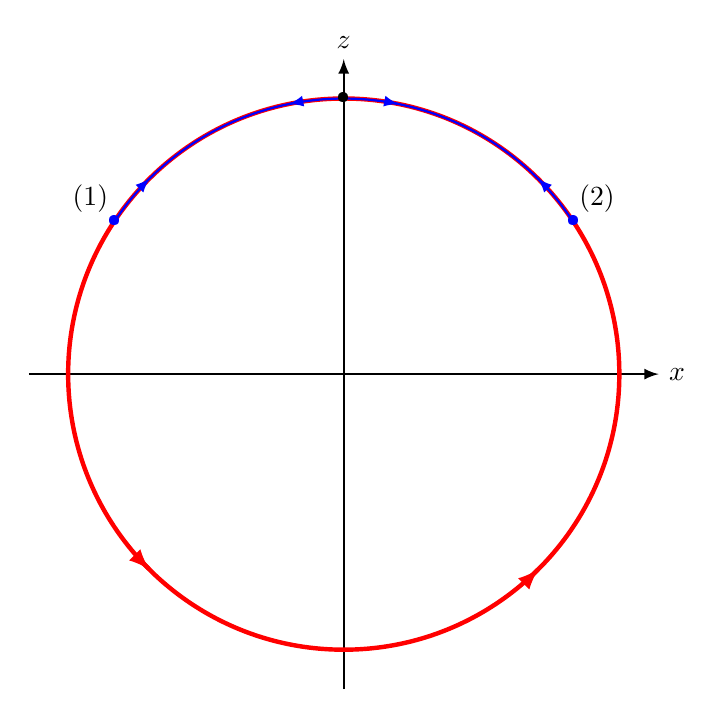
\begin{tikzpicture}
\draw[-latex, thick] ( 0.0, -4) -- (0, 4) node[above]{$z$};
\draw[-latex, thick] (-4,  0) -- (4, 0) node[right]{$x$};

\draw[red, ultra thick] (3.5, 0) arc (0:360:3.5);
\draw[-latex, red, ultra thick] (2.4648737348, -2.4848737348) -- (2.4748737348, - 2.4748737348);
\draw[-latex, red, ultra thick] (-2.4748737348, -2.4748737348) -- (-2.4648737348, -2.4848737348);

\draw[domain=33.540844097:146.459155903,smooth,variable=\x,blue, thick] plot ({3.5 * cos(\x)},{3.5 * sin(\x)});
\draw[-latex, blue, thick] (0.6853426578, 3.4322601227) -- (0.6953426578, 3.4302330223);
\draw[-latex, blue, thick] (2.4748737348,  2.4748737348) -- (2.4648737348, 2.4848737348);
\draw[-latex, blue, thick] (-0.6853426578, 3.4322601227) -- (-0.6953426578, 3.4302330223);
\draw[-latex, blue, thick] (-2.4748737348,  2.4748737348) -- (-2.4648737348, 2.4848737348);

%nodes:
\node[black] at (0, 3.5) {\textbullet};
\node[blue] at (-2.9172225397, 1.9338595227) {\textbullet};
\node[black] at (-2.9172225397 - 0.3, 1.9338595227 + 0.3) {(1)};
\node[blue] at (2.9172225397, 1.9338595227) {\textbullet};
\node[black] at (2.9172225397 + 0.3, 1.9338595227 + 0.3) {(2)};
\end{tikzpicture}
\caption{$\hat{h}(k)$ plotted as function of $k$. The angle with respect to the $z$ axis is given by $\tan(\theta_k) = \Delta^{11}_k/\varepsilon_k$.  In blue: $\mu < 0$. The blue curve starts on the north pole, at the black dot. It then goes counterclockwise until it reaches the point (1). It turns around, goes clockwise until it reaches (2). Finally it returns to the north pole. The total winding number is $w = 0$. In red: $\mu > 0$. The red curve starts and ends at the north pole, at the black dot. It goes counterclockwise around 0. The total winding number is $w = -1$. }
\label{fig.hhatplot}
\end{figure}

From equation \eqref{eq.windingnumber.Kitaevsinglewire} it is clear, that for vacuum, where $\Delta^{11}_k = 0$, the winding number is $w = 0$. Hence, this is the topologically trivial value. For nonzero pairing it turns out that there are three possibilities for the topological invariant: 
\begin{equation}
w = 2\text{CS}_{1,1} = \left\{ \begin{matrix} 
-\text{sgn}(\Delta^{11}_{k_0}) & \mu > 0, \\
0, & \mu < 0,
\end{matrix} \right. \nonumber 
\end{equation}
where $\text{sgn}$ denotes the sign function and $k_0 > 0$ is defined by $\varepsilon_{k_0} = 0$. In section \ref{subsec.2wires_CSinv_Delta12real} this result will appear as a limiting case to a more general result. The negative chemical potential case, $\mu < 0$, specifies a strong coupling phase, because the pairings strongly alters the chemical potential from the free gas one, $\epsilon_{F,0} > 0$. Here the system is topologically trivial: $w = 0$. In the same manner $\mu > 0$ specifies a weak coupling case with two possibilites, $w = \pm 1$, depending on the sign of the pairing, $\Delta^{11}_k$, at $k = k_0$. These are topologically nontrivial. This fits with the results for the Kitaev chain \cite{Alicea}. We have depicted the winding of $\hat{h}(k)$ in figure \ref{fig.hhatplot}. Here we assume, that $\Delta^{11}_k$ is negative for $k < 0$ and positive for $k > 0$. 

In the numerical analysis we will see, that in the weak coupling limit we are investigating, the chemical potential is not significantly altered from the free gas Fermi energy, hence $\mu > 0$. Now suppose that the wire has open ends, with junctions to the vacuum with $\Delta^{11}_k = 0$. From equation \eqref{eq.windingnumber.Kitaevsinglewire} it is clear, that the winding number is zero for vacuum: $w = 0$. The above topological analysis therefore shows, that when we spatially follow the transition between the wire and vacuum, the winding number must jump from $w = \pm 1$ to $w = 0$ at the boundary. Therefore, the bulk gap goes to zero at the boundary. In turn an edge state with zero energy emerges. Now suppose that we introduce perturbations, which respect the symmetries of the system. The robustness of the edge state can then be understood from the built-in particle-hole symmetry of the Hamiltonian. For the single wire the particle-hole symmetry is described by: $\mathcal{C} = \tau_1 K$, with $K$ the complex conjugation operator. Hereby the perturbed Hamiltonian $\mathcal{H}_k$ obeys: $\mathcal{C}\mathcal{H}_{k} = -\mathcal{H}_{-k}\mathcal{C}$. Let us assume, that we have a single particle energy solution in $k$: $\mathcal{H}_{k}\ket{\psi_k} = E_k\ket{\psi_k}$. We then get:
\begin{equation}
E_k\mathcal{C}\ket{\psi_k} = \mathcal{C}\mathcal{H}_{k}\ket{\psi_k} = -\mathcal{H}_{-k}\mathcal{C}\ket{\psi_k} \Rightarrow \mathcal{H}_{-k}\left(\mathcal{C}\ket{\psi_k}\right) = -E_k\left(\mathcal{C}\ket{\psi_k}\right).
\end{equation}
This shows, that if $\ket{\psi_k}$ has the energy $E_k$, then $\mathcal{C}\ket{\psi_k}$ has the energy $-E_k$. In other words for every positive energy solution there is also a negative one, as is shown to the left in figure \ref{fig.edgestates}. The perturbations may move the bulk gap, $\Delta E$, because any low energy state with $E \neq 0 $ can simply be gapped away. This is indicated in the figure by the black dots and arrows. However, the \textit{single} gapless state at $E = 0$ remains exactly there, because if it moved either up or down, there would not be the +/- symmetry in the energies. This leads to an energy spectrum, which is \textit{robust} against symmetry-conserving perturbations with the continuum above the bulk gap and a \textit{single} zero energy edge state as indicated in figure \ref{fig.edgestates}. 

\begin{figure}
\center
\begin{tikzpicture}
\draw[|-latex, thick] (0, 0) -- (0,  2) node[above]{$E$};
\draw[-, thick]   (0, 0) -- (0, -2);
\node at (-0.4, 0) {$0$};

\draw[-, dashed] (0, 1)--(1, 1);
\draw[-, thick] (-0.1, 1)--(0.1, 1);
\node at (-1.17,1) {$\phantom{min[]}\Delta E$};

\draw[-, dashed] (0, -1)--(1, -1);
\draw[-, thick] (-0.1, -1)--(0.1, -1);
\node at (-1.38,-1) {$\phantom{min[]}-\Delta E$};

\draw[-, ultra thick] (1, 1)--(1, 2);
\draw[-, ultra thick] (1, -1)--(1, -2);
\node[red] at (1, 0) {\textbullet};

\node at (1, 0.5) {\textbullet};
\draw[-latex] (1, 0.5) --  (1,  1);
\node at (1, -0.5) {\textbullet};
\draw[-latex] (1, -0.5) -- (1, -1);

\draw[-, dashed] (0,0.01) --(1,0.01);

\draw[scale=0.5,domain=-1:1,smooth,variable=\x,red, thick] plot ({\x + 6},{ 3 * exp{- 10 * \x*\x}});
\draw[scale=0.5,domain=-1:1,smooth,variable=\x,red, thick] plot ({\x + 16},{ 3 * exp{- 10 * \x*\x}});

\node at (3, -0.4) {$0$};
\node at (8, -0.4) {$\mathcal{L}$};
\draw[|-latex, thick ] (3,0) -- (9,0) node[right]{$x$};

\draw[-, ultra thick ] (3,0) -- (8,0);
\end{tikzpicture}
\caption{To the left the energy spectrum is sketched. Because of the particle-hole symmetry, there is a negative energy state for every positive. $\Delta E$ is the bulk energy gap. There is a continuum of states above $\Delta E$ and below $-\Delta E$. Any low energy state can be perturbed away, but the particle-hole symmetry protects the single state at $E = 0$, indicated by the red dot. The corresponding wave function is sketched to the right.}
\label{fig.edgestates}
\end{figure}

\subsection{Double wire, imaginary interwire pairing} \label{subsec.2wires_CSinv_Delta12imag}
In this subsection we will in detail calculate the $\mathbb{Z}$ topological invariant in the case of an imaginary interwire pairing. 

For an imaginary interwire pairing, there is only a $T^2 = + \mathbb{I}$ symmetry. The topological invariant, $\nu_{\mathbb{Z}}$, is then given by the winding number, twice the Chern-Simons invariant:
\begin{align}
\nu_{\mathbb{Z}} &= 2\text{CS}_1 = \frac{i}{\pi} \int dk\; \text{tr}[\mathcal{A}] = \frac{i}{\pi} \int dk\; \left[\bra{e^{-}_{1,k}}\partial_k\ket{e^{-}_{1,k}} + \bra{e^{-}_{2,k}}\partial_k\ket{e^{-}_{2,k}}  \right] \nonumber \\
 &= 2(\text{CS}_{1,1} + \text{CS}_{1,2})\in \mathbb{Z}, \hspace{0.5cm} T^2 = +\mathbb{I}.
\label{eq.2wires.topinv.T2eqplus1}
\end{align}
Here we have indicated the contribution to the Chern-Simons invariant from the eigenvector $\ket{e^{-}_{i,k}}$ with $\text{CS}_{1,i}$. We will refer to these as the subsystem invariants. For $T^2 = +\mathbb{I}$ the subsystem invariants are not well-defined, only their sum is. Therefore, in this situation they do not separately define an invariant, and in particular they can take non-integer values.

We now calculate $\nu_{\mathbb{Z}}$. Since we differentiate the eigenvectors with respect to $k$, it is essential that these are well-behaved in any $k$. If we look closely at the eigenvectors derived back in section \ref{sec.HFFfull}, we can see that if $\Delta^{12}_k = 0$, the eigenvectors are not well-behaved in $k = 0$. Back then this was no issue, since a single problem point in the integral makes no difference.\footnote{One might be concerned about this line of thinking. However, the gap equations in the special cases investigated in the current section have also been derived using well-behaved eigenvectors. The result is the same.} Hence, the single truly tricky part is to get well-behaved eigenvectors. However, there is a procedure for it described in \cite{Ryu.Topology}. First we transform the Hamiltonian to the standard Nambu spinor form, so that $C_k \to \tilde{C}_k = \begin{bmatrix} c_{1,k} & c_{2,k} & c^\dagger_{1,-k} & c^\dagger_{2,-k}  \end{bmatrix}^{t}$. This amounts to the following transformation of $\mathcal{H}_{FF,k}$:
\begin{align}
\mathcal{H}_{FF,k} &= \varepsilon_k \sigma_0 \otimes \tau_3 + \Delta^{11}_k \sigma_3 \otimes \tau_1 + \Delta^{12}_k \sigma_2 \otimes \tau_1 \to \nonumber \\
\mathcal{H}'_{FF,k} &= \varepsilon_k \sigma_3 \otimes \tau_0 + \Delta^{11}_k \sigma_1 \otimes \tau_3 + \Delta^{12}_k \sigma_1 \otimes \tau_2, \nonumber 
\end{align}
where $\otimes$ is the direct product and $\sigma_i, \tau_i$ are the Pauli matrices. We have also written the imaginary interwire pairing as $i\Delta^{12}_k$. Notice, that we simply flip the $\tau$ and $\sigma$ matrices. Since the Hamiltonian both has a time reversal and particle-hole symmetry, it also has a sublattice symmetry anticommuting with the Hamiltonian in first quantization: $\{\mathcal{S}, \mathcal{H}_{FF,k}\} = 0$. In the new basis after the above transformation we see, that $\mathcal{S} = \sigma_1\otimes \tau_1$. $\mathcal{S}$ has eigenvectors $v_{ab} = \chi^{1}_a\otimes \chi^{1}_b$, where $\chi^{1}_a$ for $a = 1,2$ are the eigenvectors to the first Pauli matrix $\tau_1, \sigma_1$. We then transform to the basis, where $\mathcal{S}$ is diagonal by forming $V = (v_{ab})$ and calculating:
\begin{equation}
\tilde{\mathcal{H}}_{FF,k} = V^\dagger\mathcal{H}'_{FF,k}V = \varepsilon_k \sigma_1\otimes \tau_1 + \Delta^{11}_k \sigma_1\otimes\tau_3 - \Delta^{12}_k\sigma_2\otimes\tau_0. \nonumber 
\end{equation}
We then get the eigenvectors to negative energy eigenvalues:
\begin{equation}
\ket{e^{-}_{1,k}} = \frac{1}{2E_{F,k}}\begin{bmatrix} \varepsilon_k + i(\Delta^{11}_k + i\Delta^{12}_k) \\ i\left(\varepsilon_k + i\left(\Delta^{11}_k - i\Delta^{12}_k\right)\right) \\ -iE_{F,k} \\ -E_{F,k} \end{bmatrix}, \hspace{0.5cm} \ket{e^{-}_{2,k}} = \frac{1}{2E_{F,k}}\begin{bmatrix} \varepsilon_k + i(-\Delta^{11}_k - i\Delta^{12}_k) \\ -i\left(\varepsilon_k + i\left(-\Delta^{11}_k + i\Delta^{12}_k\right)\right) \\ iE_{F,k} \\ -E_{F,k} \end{bmatrix},
\end{equation}
with $E_{F,k} = \sqrt{\varepsilon_k^2 + (\Delta^{11}_k)^2 + (\Delta^{12}_k)^2}$. These eigenvectors are manifestly well-defined for all $k$. Using these we explicitly get:
\begin{equation}
\mathcal{A}^{11}_k = \bra{e^{-}_{1,k}}\partial_k\ket{e^{-}_{1,k}} = -\frac{i}{2E_{F,k}^2}(\Delta^{11}_k\partial_k\varepsilon_k - \varepsilon_k\partial_k\Delta^{11}_k) = -\mathcal{A}^{22}_k. \nonumber
\end{equation}
Hereby: $\text{tr}[\mathcal{A}_k] = \mathcal{A}^{11}_k  + \mathcal{A}^{22}_k = 0$, and the topological invariant is simply $\nu_{\mathbb{Z}} = 0$. Since $\mathcal{A}^{11}_k$ vanishes for $\Delta^{11}_k = \Delta^{12}_k = 0$, $\nu_{\mathbb{Z}} = 0$ is the topologically trivial value. We will later see, what physical consequences this has by studying the edge states. We emphasize, that the subsystem "invariants" given by $2\text{CS}_{1,j} = \frac{i}{\pi}\int dk \mathcal{A}^{jj}_k$ are not well-defined separately. In the present context it means, that they take non-integer values during the cross over, where both $\Delta^{11}_k$ and $\Delta^{12}_k$ are present. Only their sum, here equal to $0$, gives a topological invariant. Later we will numerically calculate these subsystem "invariants". From the above, they become:
\begin{equation}
\text{CS}_{1,1} = - \text{CS}_{1,2} = \frac{1}{4\pi}\int dk \; \frac{\Delta^{11}_k\partial_k\varepsilon_k - \varepsilon_k\partial_k\Delta^{11}_k}{\varepsilon^2_k + (\Delta^{11}_k)^2 + (\Delta^{12}_k)^2}. 
\end{equation}
These are continuous functions of $\Delta^{11}_k, \Delta^{12}_k$ and $\varepsilon_k$. Notice, that for the uncoupled wires, $\Delta^{12}_k = 0$, we retrieve the winding number, $w$, for the single wire as discussed in the previous subsection. 


\subsection{Double wire, real interwire pairing} \label{subsec.2wires_CSinv_Delta12real}
In this subsection we calculate the topological invariants in the case of a real interwire pairing. 

For a real interwire pairing the system both has a $T^2 = +\mathbb{I}$ and $T^2 = -\mathbb{I}$ symmetry. The former is given by $T_2$ of section \ref{subsec.TRseparatewires}, which only exchange particles within the same wire. The latter is given by $T_-$ of section \ref{subsec.TRwireexchange}, which exchanges particles between the two wires. Therefore, the system both has $\mathbb{Z}$ and $\mathbb{Z}_2$ invariant. The $\mathbb{Z}$ invariant is given by equation \eqref{eq.2wires.topinv.T2eqplus1}.

The $\mathbb{Z}_2$ invariant is connected to the $T^2 = -\mathbb{I}$ symmetry. For such a time reversal symmetry, the states of the system come in time reversal, or Kramers, pairs. We will see this explicitly later on. At the present stage this means, that the subsystem invariants $\text{CS}_{1,i}$ of  \eqref{eq.2wires.topinv.T2eqplus1} \textit{are} separately well-defined and it is meaningful to calculate their respective values \cite{FuKane2006, LiYangChen} and \cite[pp. 130-135]{BernevigTITSC}. The $\mathbb{Z}_2$ invariants can then be calculated by going to the socalled Wilson loop:
\begin{equation}
\nu_{\mathbb{Z}_2} = W_{1,j} = \text{e}^{2\pi i\text{CS}_{1,j}} = \pm 1, \hspace{0.5cm} T^2 = -\mathbb{I}.
\label{eq.2wires.topinv.T2eqminus1}
\end{equation}
We are now ready for the computation. To get to well-behaved eigenvectors we follow the same procedure as outlined in the previous subsection. The $\Delta^{12}_k$ term of $\mathcal{H}_{FF,k}$ now has the form $\Delta^{12}_k \sigma_2 \otimes \tau_2$. After going to the Nambu spinor form, we therefore have $\mathcal{H}'_{FF,k} = \varepsilon_k \sigma_3 \otimes \tau_0 + \Delta^{11}_k \sigma_1 \otimes \tau_3 + \Delta^{12}_k \sigma_2 \otimes \tau_2$. The anticommuting sublattice symmetry is now given by: $\mathcal{S} = \sigma_1\otimes \tau_2$. The corresponding eigenvectors are therefore $v_{ab} = \chi^{1}_a\otimes\chi^{2}_b$. Letting $V = (v_{ab})$ and calculating the conjugation of $\mathcal{H}'_{FF,k}$ then yields:
\begin{equation}
\tilde{\mathcal{H}}_{FF,k} = V^\dagger\mathcal{H}'_{FF,k}V = \varepsilon_k \sigma_1\otimes \tau_1 + \Delta^{11}_k \sigma_1\otimes\tau_3 - \Delta^{12}_k\sigma_2\otimes\tau_1. \nonumber 
\end{equation}
To calculate the $\mathbb{Z}$ topological invariant, we need both negative energy eigenvectors:
\begin{equation}
\ket{e^{-}_{1,k}} = \frac{1}{2E^{+}_{F,k}}\begin{bmatrix} \varepsilon_k + i(\Delta^{11}_k + \Delta^{12}_k) \\ i(\varepsilon_k + i(\Delta^{11}_k + \Delta^{12}_k)) \\ -iE^{+}_{F,k} \\ -E^{+}_{F,k} \end{bmatrix}, \hspace{0.5cm} \ket{e^{-}_{2,k}} = \frac{1}{2E^{-}_{F,k}}\begin{bmatrix} \varepsilon_k + i(-\Delta^{11}_k + \Delta^{12}_k) \\ -i(\varepsilon_k + i(-\Delta^{11}_k + \Delta^{12}_k)) \\ iE^{-}_{F,k} \\ -E^{-}_{F,k} \end{bmatrix}. \nonumber
\end{equation}
These are seen to be manifestly well-defined for all $k$. Notice, that these eigenvectors are different from the ones for an imaginary interwire pairing, $\Delta^{12}_k$, in two ways. First, for a real interwire pairing the energies $E^{\pm}_{F,k}$ are in general different. Second, the front factors of $\Delta^{12}_k$ are altered. Since the entries of $\ket{e^{-}_{2,-k}}$ and $\ket{e^{-}_{1,+k}}$ are equal up to a sign, we get that:
\begin{equation}
\mathcal{A}^{11}_k = \bra{e^{-}_{1,k}}\partial_k\ket{e^{-}_{1,k}} = \bra{e^{-}_{2,-k}}\partial_k\ket{e^{-}_{2,-k}} = - \bra{e^{-}_{2,-k}}\partial_{-k}\ket{e^{-}_{2,-k}} = -\mathcal{A}^{22}_{-k}. \nonumber
\end{equation}
Hence, $\text{CS}_{1,2} = - \text{CS}_{1,1}$. The $\mathbb{Z}$ topological invariant is then trivial: $\nu_{\mathbb{Z}} = 2(\text{CS}_{1,1} + \text{CS}_{1,2}) = 0$. The $\mathbb{Z}_2$ invariants are now calculated. First, we get:
\begin{equation}
\mathcal{A}^{11}_k = \bra{e^{-}_{1,k}}\partial_k\ket{e^{-}_{1,k}} = \frac{i}{2(E^{+}_{F,k})^2}\left(\varepsilon_k\partial_k(\Delta^{11}_k + \Delta^{12}_k) - (\Delta^{11}_k + \Delta^{12}_k)\partial_k \varepsilon_k\right) \nonumber
\end{equation}
The subsystem invariants are then:
\begin{equation}
\text{CS}_{1,1} = - \text{CS}_{1,2} = \frac{1}{4\pi}\int dk \; \frac{\varepsilon_k\partial_k(\Delta^{11}_k + \Delta^{12}_k) - (\Delta^{11}_k + \Delta^{12}_k)\partial_k \varepsilon_k}{\varepsilon_k^2 + (\Delta^{11}_k + \Delta^{12}_k)^2}.
\label{eq.CS11integralform}
\end{equation}
The integrand has a quite simple primitive:
\begin{equation}
\theta_k(c) = \arctan\left(\frac{\Delta^{11}_k + \Delta^{12}_k }{\varepsilon_k}\right) + c,
\label{eq.thetak.def}
\end{equation}
where $c$ is a constant. The evaluation of the integral itself however turns out to be a little subtle. There are two cases.

$\boldsymbol\mu \;\mathbf{< 0}$: $\varepsilon_k = \frac{k^2}{2m_F} - \mu$ is strictly positive for any $k$. This means, that $\arctan\left(\frac{\Delta^{11}_k + \Delta^{12}_k }{\varepsilon_k}\right)$ is well-defined for all $k$ and we can use $\theta_k(c = 0)$ as the primitive. Then:
\begin{equation}
\text{CS}_{1,1} = \frac{1}{4\pi}\left.\arctan\left(\frac{\Delta^{11}_k + \Delta^{12}_k }{\varepsilon_k}\right)\right|^{\infty}_{-\infty} = 0, \nonumber
\end{equation}
as both $\Delta^{11}_k$ and $\Delta^{12}_k$ goes to $0$ and $\varepsilon_k \to \infty$ for $k\to \pm \infty$, and $\arctan(0) = 0$. This behaviour of the pairings is explicitly shown in the numerical analysis. Hence, for $\mu < 0$ we get $\nu = \text{e}^{2\pi i\text{CS}_{1,1}} = 1$ and the system is topologically trivial. 

$\boldsymbol\mu \; \mathbf{> 0}$: $\varepsilon_k$ has two zero points at the Fermi surface $k = \pm k_0$. This introduces discontinuities in $\theta_k(c = 0)$ at $\pm k_0$. However, for the evaluation of the integral to be correct, we must use a continuous primitive. Therefore we have to patch a continuous solution together by looking in the intervals $k < -k_0, -k_0 < k < +k_0$ and $k > +k_0$. Since $E^{\pm}_{F,k} \neq 0$ for all $k$ and $\varepsilon_{\pm k_0} = 0$, we get that $\Delta^{11}_{\pm k_0} + \Delta^{11}_{\pm k_0} \neq 0$. If this was not the case, the energy gap would close at either $+k_0$ or $-k_0$ and the topological index would be ill-defined. This means, that $\text{sgn}(\Delta^{11}_k + \Delta^{12}_k)$ is well-defined in $k = \pm k_0$. By taking the limits around $\pm k_0$ of $\theta_k(c = 0)$ we can see, that the following construction is a continuous primitive to the integrand in equation \eqref{eq.CS11integralform}:
\begin{equation}
\theta_k = \left\{ \begin{matrix} 
\arctan\left(\frac{\Delta^{11}_k + \Delta^{12}_k }{\varepsilon_k}\right) - \pi\text{sgn}(\Delta^{11}_{k_0} + \Delta^{12}_{k_0}), & k > k_0, \\
\arctan\left(\frac{\Delta^{11}_k + \Delta^{12}_k }{\varepsilon_k}\right), & -k_0 \leq k \leq k_0, \\
\arctan\left(\frac{\Delta^{11}_k + \Delta^{12}_k }{\varepsilon_k}\right) - \pi \text{sgn}(-\Delta^{11}_{k_0} + \Delta^{12}_{k_0}), & k < -k_0.
  \end{matrix} \right.
\label{eq.2wires.Gkmugreater0}
\end{equation}
We expect, that the pairings go to zero for $k\to \pm \infty$. We will verify this in the numerical analysis. Since $\varepsilon_k \overset{k\to \pm \infty}{\to} \infty$, the $\arctan$ part of $\theta_k$ goes to zero in these limits. Further, this means, that the signs $\text{sgn}(\Delta^{11}_{\pm k_0} + \Delta^{12}_{\pm k_0})$ must be different for the integral to give a nonzero result. Since $\Delta^{12}_{k}$ is even and $\Delta^{11}_{k}$ is odd, this can only be achieved if $\Delta^{11}_{k}$ is dominant at the Fermi points: $|\Delta^{11}_{k_0}| > |\Delta^{12}_{k_0}|$. Hence, we get:
\begin{equation}
\text{CS}_{1,1} = \left. \frac{1}{4\pi} \theta_k \right|^\infty_{-\infty} = -\frac{1}{4}(\text{sgn}(\Delta^{11}_{k_0} + \Delta^{12}_{k_0}) - \text{sgn}(-\Delta^{11}_{k_0} + \Delta^{12}_{k_0})) = \left\{ \begin{matrix} 
-\frac{1}{2}\text{sgn}(\Delta^{11}_{k_0} + \Delta^{12}_{k_0}) , & |\Delta^{11}_{k_0}| > |\Delta^{12}_{k_0}|, \\
0, & |\Delta^{11}_{k_0}| < |\Delta^{12}_{k_0}|.
  \end{matrix} \right. \nonumber 
\end{equation}
This is the form we used for the winding number in subsection \ref{subsec.topologicalinvariant.singlewire} for $\Delta^{12}_k = 0$. The above results in the $\mathbb{Z}_2$ invariant:
\begin{equation}
\nu_{\mathbb{Z}_2} = \text{e}^{2\pi i \text{CS}_{1,1}} = \text{e}^{2\pi i \text{CS}_{1,2}} = \left\{ \begin{matrix} 
-1, & |\Delta^{11}_{k_0}| > |\Delta^{12}_{k_0}| & \text{and} & \mu > 0, \\
+1, & |\Delta^{11}_{k_0}| < |\Delta^{12}_{k_0}| & \text{or}  & \mu < 0.
  \end{matrix} \right.
\label{eq.CS11T2eqminus1}
\end{equation}
Hence, to be in a topological nontrivial phase we need to be in the weak coupling phase, $\mu > 0$. Further the intrawire pairing, $\Delta^{11}_k$, \textit{must} be dominant at the Fermi surface points $k = \pm k_0$, where $\varepsilon_{\pm k_0} = 0$. 

As a by-product of this subsection, we get that in the $d \to 0$ limit, the system is topologically trivial, since $\Delta^{12}_k$ is dominant here. This shows explicitly, that a system with only $s$-wave pairing is topologically trivial. 

\section{Edge states and Kramers degeneracy} \label{sec.edgestatesandkramers}
In this section we will go into more detail with the edge states. We calculate approximate solutions for these in the case of uncoupled wires. We then go beyond mean field theory to address the question of how the interwire interaction influences these edge states. This is connected to Kramers degeneracy of time reversal partners.  

\subsection{Edge states: approximate solutions}
\label{subsec.2wiresedgestates}
We have now seen, that a nonzero topological index leads to the existence of gapless edge states. Here we will explicitly show, how these edge states emerge for the uncoupled wires. The analysis is largely based on \cite[pp. 196-198]{BernevigTITSC}. 

\begin{figure}
\center
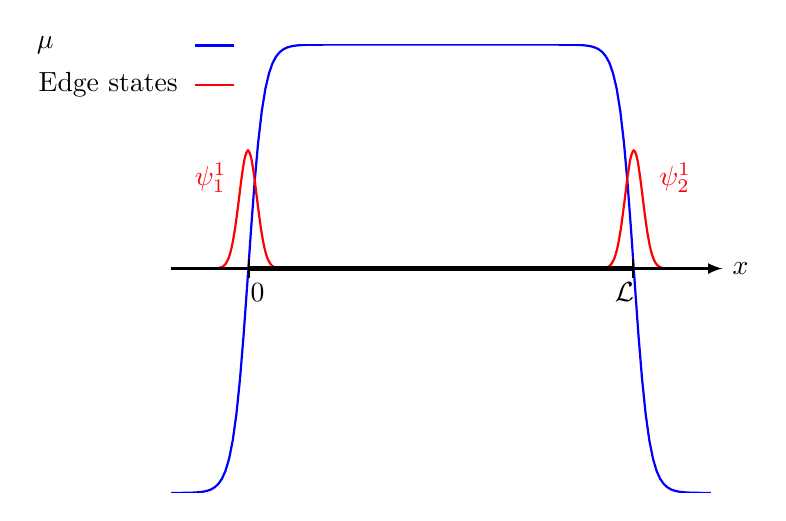
\begin{tikzpicture}
\begin{axis}[samples=150, xtick=\empty, ytick=\empty, axis line style={draw=none}, 
    xmin=-1, xmax=6,
    ymin = -1/2, ymax = 1/2,
    axis lines=center,
    domain=-1:6,
    ]

    \addplot [mark=none,draw=blue, thick] {1/2 * (tanh(5 * \x) - tanh(5 * (\x - 5) ) - 1)};
\end{axis}


\draw[scale=0.5,domain=-1:1,smooth,variable=\x,red, thick] plot ({\x + 0.975 * 2},{ 2 * 2.85 + 3 * exp{- 10 * \x*\x}});
\draw[scale=0.5,domain=-1:1,smooth,variable=\x,red, thick] plot ({\x + 5.875 * 2},{ 2 * 2.85 + 3 * exp{- 10 * \x*\x}});

\node at (0.975 + 0.12, 2.85 - 0.3) {$0$};
\node at (5.875-0.12, 2.85 - 0.3) {$\mathcal{L}$};
\draw[-latex, thick ] (0,2.85) -- (7,2.85) node[right]{$x$};
\draw[-, ultra thick ] (0.975,2.85) -- (5.875,2.85);
\draw[|-, thick ] (0.975,2.85) -- (1,2.85);
\draw[-, ultra thick ] (0.975,2.85) -- (5.875,2.85);
\draw[-|, thick ] (5.7,2.85) -- (5.875,2.85);

\coordinate (a) at (0.3, 5.682);
\coordinate (anode) at (-1.6, 5.682);
\coordinate (b) at (0.8, 5.682);
\coordinate (c) at (0.3, 5.182);
\coordinate (d) at (0.8, 5.182);
\coordinate (cnode) at (-0.8, 5.182);
\coordinate (wavefunctionnode11) at (0.5, 4.0);
\coordinate (wavefunctionnode12) at (6.4, 4.0);

\draw[-, thick, blue] (a) -- (b);
\node at (anode) {$\mu$}; 
\draw[-, thick, red] (c) -- (d);
\node at (cnode) {Edge states}; 
\node[red] at (wavefunctionnode11) {$\psi^{1}_{1}$};
\node[red] at (wavefunctionnode12) {$\psi^{1}_{2}$};
\end{tikzpicture}
\caption{Red: Edge states. Blue: chemical potential $\mu = \mu(x)$. Due to the spatial variation of the chemical potential the fermions are confined to the interval between $x = 0$ and $x = \mathcal{L}$. The uncoupled wires are topological for $\mu > 0$. For $\mu < 0$ they are trivial. Hence, edge states form around $\mu = 0$ at $x = 0$ and $x = \mathcal{L}$. Since the wires are uncoupled we only show one of them.}
\label{fig.edgestatesmux}
\end{figure}

We would like to describe the Hamiltonian in real space, because we now ask whether certain states exist at the ends of the wires. To do this we define the operator $\Delta^{11}(p)$ as a function of the momentum operator $p = -i\partial_x$ in the following manner:
\begin{equation}
\Delta^{11}(p)\text{e}^{ikx} = \Delta^{11}_k\text{e}^{ikx}.
\label{eq.Deltapdef}
\end{equation}
Hence, we replace the variable dependency of $k$ in $\Delta^{11}_k$ with an operator dependency on $p$ in $\Delta^{11}(p)$. With this definition we get the Hamiltonian in real space:
\begin{equation}
H_{FF} = \frac{1}{2}\int dx\; \Psi^\dagger_{F}(x) \mathcal{H}_{FF}(x) \Psi_{F}(x), \hspace{0.5cm} \Psi_{F}(x) = \begin{bmatrix} \psi_{1,F}(x) & \psi^\dagger_{1,F}(x) & \psi_{2,F}(x) & \psi^\dagger_{2,F}(x)\end{bmatrix}^t
\label{eq.2wiresMFHamiltonianrealspace}
\end{equation}
With the real space Hamiltonian kernel:
\begin{equation}
\mathcal{H}_{FF}(x) = \begin{bmatrix} 
\frac{p^2}{2m_F} - \mu & \Delta^{11}(p) & 0 & 0 \\
\Delta^{11}(p) & -\left(\frac{p^2}{2m_F} - \mu \right) & 0 & 0 \\
0 & 0 & \frac{p^2}{2m_F} - \mu & -\Delta^{11}(p) \\
0 & 0 & -\Delta^{11}(p) & -\left(\frac{p^2}{2m_F} - \mu \right)
\end{bmatrix}.
\label{eq.2wiresMFHamiltonianrealspacefirstquantization}
\end{equation}
For the sake of clarity let us see how e.g. the term $\Delta^{11}_kc_{1,-k}c_{1,k}$ appears from this expression:
\begin{align}
\int dx \; \psi_{1,F}(x) \Delta^{11}(p) \psi_{1,F}(x) &= \frac{1}{\mathcal{L}}\sum_{k,q}c_{1,k} c_{1,q}\int dx \; \text{e}^{ikx}\Delta^{11}(p)\text{e}^{iqx} = \frac{1}{\mathcal{L}}\sum_{k,q}\Delta^{11}_qc_{1,k}c_{1,q}\int dx \; \text{e}^{i(k + q)x} \nonumber \\
&= \sum_{k}\Delta^{11}_kc_{1,-k}c_{1,k}, \nonumber 
\end{align}
since $\int dx\; \text{e}^{i(k + q)x} =\mathcal{L} \delta_{k,-q} $. Here we use the Fourier decomposition $\psi_{1,F}(x) = \frac{1}{\sqrt{L}}\sum_k\text{e}^{ikx}c_{1,k}$. Now we form junctions of topogically distinct phases by changing the sign of $\mu$ at $x = 0$ and $x = \mathcal{L}$. Hence, we let $\mu = \mu(x)$ as shown in figure \ref{fig.edgestatesmux}. Due to the spatial variation of the chemical potential the fermions are confined to the wire between $x = 0$ and $x = \mathcal{L}$. In first quantization we find solutions by solving $\mathcal{H}(x)\psi(x) = E\psi(x)$. The edge states are zero energy modes, so we solve for $E = 0$. We assume, that $\mu(x)$ varies slowly over the interparticle length scale $1/k_F$. When this is fulfilled the solution $\psi(x)$ will also vary slowly and hence the curvature of $\psi(x)$ proportional to $p^2\psi(x)$ is negligible. This means, that to a good approximation we only keep the operator $p$ up to first order. Since the intrawire pairing, $\Delta^{11}_k$, is $p$-wave type, it is linear in $k$ for $k/k_F \ll 1$. We will also verify this in the numerical analysis in chapter \ref{Chapter6}. This means, that $\Delta^{11}(p)$ is linear in $p$, when $p/k_F$ used on a state is small. Hence, we ignore $p^2/2m_F$ and let $\Delta^{11}(p) = \Delta^{11} \cdot \tilde{p}$, with $\Delta^{11} = k_F\left.\frac{\partial \Delta^{11}_k}{\partial k}\right|_{k=0}$ and $\tilde{p} = p/k_F$. We assume $\Delta^{11} > 0$. We take the ansatz:
\begin{equation}
\psi^{i}_1(x) = \exp\left(-\frac{k_F}{\Delta^{11}}\int_{0}^{x} dx'\; \mu(x') \right)\mathbf{u}^{i}_{1}, \hspace{0.5cm} \psi^{i}_2(x) = \exp\left(+\frac{k_F}{\Delta^{11}}\int_{\mathcal{L}}^{x} dx'\; \mu(x') \right)\mathbf{u}^{i}_{2}, \nonumber
\end{equation}  
The superscript ${}^i$ refers to the wire, the subscript ${}_{1,2}$ to which end the wave function is located. Since $\Delta^{11}$ is in units of energy the exponents are unitless. Since $\Delta^{11} > 0$, we see that these states are exponentially localized at the edges. From this we get eigenvalue equations for $\mathbf{u}^{i}_{j}$. Defining $g_1(x) = \frac{1}{N}\text{e}^{-\frac{k_F}{\Delta^{11}}\int_{0}^{x} dx' \mu(x')}$, $g_2(x) = \frac{1}{N}\text{e}^{+\frac{k_F}{\Delta^{11}}\int_{\mathcal{L}}^{x} dx' \mu(x')}$ and $N^2 = \int dx |g_j(x)|^2$ a normalization constant we hereby get the approximate solutions:
\begin{align}
\psi^1_1(x) &= g_1(x)\frac{\text{e}^{+i\pi/4}}{\sqrt{2}}\begin{bmatrix} 1 & -i & 0 & 0 \end{bmatrix}^t , \hspace{0.5cm} \psi^1_2(x) = g_2(x)\frac{\text{e}^{-i\pi/4}}{\sqrt{2}}\begin{bmatrix} 1 & +i & 0 & 0 \end{bmatrix}^t, \nonumber \\
\psi^2_1(x) &= g_1(x)\frac{\text{e}^{-i\pi/4}}{\sqrt{2}}\begin{bmatrix} 0 & 0 & 1 & +i \end{bmatrix}^t , \hspace{0.5cm} \psi^2_2(x) = g_2(x)\frac{\text{e}^{+i\pi/4}}{\sqrt{2}}\begin{bmatrix} 0 & 0 & 1 & -i \end{bmatrix}^t.
\end{align}
These states solve $\mathcal{H}_{FF}\psi(x) = 0$. I.e. they have zero energy. They are the explicit forms of the gapless edge states. From equation \eqref{eq.2wiresTminuswireexchangefirstquantization} we have, that the time reversal operator that squares to minus the identity is given by: $\mathcal{T}_- = i\sigma_2\otimes\tau_0 \cdot K$. Hence, $\mathcal{T}_-\psi^1_1(x) = -\psi^2_1(x)$ and $\mathcal{T}_-\psi^1_2(x) = -\psi^2_2(x)$. The edge states at the same end in each wire are therefore Kramers partners. This is crucial for the following analysis. For sake of completeness let us write up the second quantized version of the four states. The eigenstates define the diagonalisation matrix $U(x) = \begin{bmatrix} \psi^{1}_{1}(x) & \psi^{1}_{2}(x) & \psi^{2}_{1}(x) & \psi^{2}_{2}(x) \end{bmatrix}$. This has the unitarity property, that $\int dx \; U^\dagger(x) U(x) = \mathbb{I}$. We then let the operators $\gamma^{j}_{1}, \gamma^{j}_{2}$ for wire $j$ be given by:
\begin{equation}
\begin{bmatrix} \psi_{1,F}(x) \\ \psi_{1,F}^\dagger(x) \\ \psi_{2,F}(x) \\ \psi_{2,F}^\dagger(x) \end{bmatrix} = U(x) \begin{bmatrix} \gamma^{1}_{1} \\ \gamma^{1}_{2} \\ \gamma^{2}_{1} \\ \gamma^{2}_{2} \end{bmatrix} \Rightarrow \begin{bmatrix} \gamma^{1}_{1} \\ \gamma^{1}_{2} \\ \gamma^{2}_{1} \\ \gamma^{2}_{2} \end{bmatrix} = \int dx \; U^\dagger(x) \begin{bmatrix} \psi_{1,F}(x) \\ \psi_{1,F}^\dagger(x) \\ \psi_{2,F}(x) \\ \psi_{2,F}^\dagger(x) \end{bmatrix}.
\label{eq.Majoranaedgemodedef} 
\end{equation} 
Written out these operators are: 
\begin{align}
\gamma^1_{1} &= \int dx \; g_1(x)\frac{\text{e}^{-i\pi/4}}{\sqrt{2}}(\psi_{1,F}(x) + i\psi^\dagger_{1,F}(x)), \hspace{0.5cm} \gamma^1_{2} = \int dx \; g_2(x)\frac{\text{e}^{+i\pi/4}}{\sqrt{2}}(\psi_{1,F}(x) - i\psi^\dagger_{1,F}(x)), \nonumber \\
\gamma^2_{1} &= \int dx \; g_1(x)\frac{\text{e}^{+i\pi/4}}{\sqrt{2}}(\psi_{2,F}(x) - i\psi^\dagger_{2,F}(x)), \hspace{0.5cm} \gamma^2_{2} = \int dx \; g_2(x)\frac{\text{e}^{-i\pi/4}}{\sqrt{2}}(\psi_{2,F}(x) + i \psi^\dagger_{2,F}(x)). \nonumber 
\end{align}
In this manner $\psi^{i}_{j}(x)$ and $\gamma^{i}_{j}\ket{\text{S}}_0$ are equivalent. These operators are special in the sense, that they are their own antiparticle: $\left(\gamma^{i}_{j}\right)^\dagger = \gamma^{i}_{j}$.\footnote{This also illuminates why we chose the rather arbitrary phase factors $\text{e}^{\pm i\pi/4}$. Had we \textit{not} done this, there would be some phase difference between $\left(\gamma^{i}_{j}\right)^\dagger$ and $\gamma^{i}_{j}$.} Such a fermionic particle is called a Majorana mode in condensed matter physics. Besides being their own antiparticle, they have to obey the modified anticommutator relation:
\begin{equation}
\{\gamma^{i_1}_{j_1}, \gamma^{i_2}_{j_2} \} = \delta_{i_1,i_2}\delta_{j_1,j_2}. \nonumber
\end{equation}
This is explicitly verified to be the case for the above operators.\footnote{Often one also meets the requirement, that the anticommutator equals $2\delta_{i_1,i_2}\delta_{j_1,j_2}$. This is simply a matter of convention.} From this we can form regular fermionic operators: $d_j = \frac{1}{\sqrt{2}}(\gamma^{j}_{1} + i\gamma^{j}_{2})$. The fermionic states have equal weights in both end of each wire, which can be separated by a macroscopic distance. They are therefore highly non-local. The key result of this section is thus, that $\ket{\text{S}}_0$ and $d_j^\dagger\ket{\text{S}}_0$ are degenerate ground states of the system. The topologically non-trivial state is therefore characterized by the presence of \textit{one} more particle than the trivial one, which is exponentially located on the edges.\footnote{In the literature one also meets the notion of a Majorana mode at each end, hence two in total. However, since $\gamma^\dagger_0\gamma_0 = \gamma_0^2 = \frac{1}{2}$ for Majorana operators, we cannot count them. Hence, the notion of a specific number of Majorana modes is undefined.}

In second quantization the above notion of Kramers partners is described by the fact, that: $T_-\gamma^1_{j}T_-^{-1} = \gamma^2_{j}$, simply because $\psi_{1,F}(x) \overset{T_-}{\to} \psi_{2,F}(x)$ and $T_-$ is antiunitary.

\subsection{Kramers degeneracy: protection of edge states}
\label{sec.2wireskramersdegeneracy}
Our analysis so far has been based on the mean-field BCS Hamiltonian. Here we want to go a little further and show that Kramers theorem protects the edge states in the two wires from becoming gapped by the interwire coupling, as long as it obeys the time reversal symmetry $T^2 = -\mathbb{I}$. 

Consider a general system described by the Hamiltonian $H$. Assume, that this Hamiltonian is time reversal invariant, $[T, H] = 0$, and that $T^2 = -\mathbb{I}$. Let $\ket{\psi_1}$ and $\ket{\psi_2}$ be eigenstates to the Hamiltonian, with energy $E_1$ and $E_2$, and Kramers partners: $\ket{\psi_2} = T\ket{\psi_1}$. Since $[T, H] = 0$ the two states have the same energy: 
\begin{equation}
E_2\ket{\psi_2} = HT\ket{\psi_1} = TH\ket{\psi_1} = E_1\ket{\psi_2}. \nonumber
\end{equation}
So $E_2 = E_1$. Further, the states are orthogonal:
\begin{equation}
\braket{\psi_1|\psi_2} = \braket{T\psi_2|T\psi_1} = \braket{-\psi_1|\psi_2} = -\braket{\psi_1|\psi_2} \Rightarrow \braket{\psi_1|\psi_2} = 0. \nonumber  
\end{equation}
In the first equality we use, that we can flip the inner product by going to the time reversed states \cite[p. 274]{Sakurai}. In the second equality we use, that $T\ket{\psi_2} = -\ket{\psi_1}$, since $T^2 = -\mathbb{I}$. Hence, any energy state in a time reversal invariant system with $T^2 = -\mathbb{I}$ is twofold degenerate. This is Kramers degeneracy. Now let $H'$ be a perturbation to the Hamiltonian, which respects the time reversal symmetry: $[T, H'] = 0$. In degenerate perturbation theory we calculate the matrix with entries $W_{ij} = \bra{\psi_i}H'\ket{\psi_j}$. The eigenstates of $H$ remain good eigenstates if the states uncouple: $\bra{\psi_1}H'\ket{\psi_2} = 0$, so that $W_{ij}$ is diagonal. This is exactly the case for Kramers partners: 
\begin{equation}
\bra{\psi_1}H'\ket{\psi_2} = \bra{T\psi_2}TH'T^{-1}\ket{T\psi_1} = \bra{T\psi_2}H'\ket{T\psi_1} = -\bra{\psi_1}H'\ket{\psi_2} \Rightarrow \bra{\psi_1}H'\ket{\psi_2} = 0. \nonumber
\end{equation}
The first equality holds, since $H'$ is hermitian \cite[p. 274]{Sakurai}. 

Now what has this to do with the system at hand? We let $\ket{\psi_{i}^{j}} = \gamma_{i}^{j}\ket{\text{S}}_0$ for $i, j = 1, 2$. In this way, $\ket{\psi_{1}^1}$ is the edge state in wire 1 at end 1, $\ket{\psi_{2}^1}$ in wire 1 at end 2, and so forth. From above we know, that the edge states at end $i$, $\ket{\psi_{i}^1}$ and $\ket{\psi_{i}^2}$, are Kramers partners. If we can show, that the interwire interaction $H' = H^\text{int}_{FF,12}$ is time reversal invariant under $T_-$, then the above analysis shows that the edge states at the same end of the wire cannot couple. From equation \eqref{eq.Hint12realspace} we have:
\begin{equation}
H^\text{int}_{FF,12} = \int dx_1 dx_2 \psi^\dagger_{1,F}(x_1)\psi^\dagger_{2,F}(x_2) \tilde{V}_{\text{ind}}^{12}(x_1-x_2,0) \psi_{2,F}(x_2)\psi_{1,F}(x_1),
\end{equation}
with $\tilde{V}_{\text{ind}}^{12}(x_1-x_2,0)$ the zero frequency induced interaction in real space. Now $T_-\psi_{1,F}(x)T^{-1}_- = \psi_{2,F}(x)$ and $T_-\psi_{2,F}(x)T^{-1}_- = -\psi_{1,F}(x)$. Finally, $\tilde{V}_{\text{ind}}^{12}(x, 0)$ is real, so we get that $T_-H^\text{int}_{FF,12}T_-^{-1} = H^\text{int}_{FF,12}$. Hence, the edge states at the same end of the wire cannot couple. Further, the edge states at opposite ends of the wire are macroscopically separated. Therefore, these cannot couple either. In conclusion, the edge state in each wire is protected, as long as the interwire interaction is a perturbation to the system, which is to say no interwire mean field has formed.  

\section{Qualitative understanding of cross over}
\label{sec.2wirestransitionqualitative}
In this section we come with a qualitative analysis of how the cross over from $p$- to $s$-wave can occur using the previous two sections. 

$\mathbf{\Delta^{12}_k = 0}$: For the uncoupled wires the previous section shows, that there is a single edge state in each wire. As the wires are brought closer together, the interwire interaction, $H^\text{int}_{FF,12}$, kicks in. Before any mean field of the interwire pairing has been chosen, the previous section further shows, that the edge states stay uncoupled. This is the top of figure \ref{fig.2wiresedgestates}. 

\textbf{Imaginary interwire pairing}: Assume that as the wires are brought closer together, the system chooses the interwire pairing to be \textit{imaginary}. Then the system \textit{breaks} the time reversal symmetry $T_-$. In this case there is no longer a Kramers degeneracy. As a consequence the edge states can couple and gap away. We can actually calculate by how much the edge states gap. In this connection we define the operator $\Delta^{12}(p)$ as: $\Delta^{12}(p)\text{e}^{ikx} = \Delta^{12}_k\text{e}^{ikx}$. Since $\Delta^{12}_k$ is even in $k$, there is no first order term in $k$. Hence for states with small curvatures like the edge states we can approximate $\Delta^{12}(p) = \Delta^{12}_{k=0}$. This means, that the perturbation in real space relevant for the edge states is:
\begin{equation}
\mathcal{H}'_{FF}(x) = \Delta^{12}_{k=0}\begin{bmatrix} 
0 & 0 &  0 & -i \\
0 & 0 & -i & 0 \\
0 & i & 0  & 0 \\
i & 0 & 0  & 0  \end{bmatrix}
\label{eq.interwirepairingrealspace}
\end{equation}
The edge states in wires 1 and 2 in first quantization are described by the wave functions $\psi^1_1, \psi^2_1, \psi^1_2, \psi^2_2$ found in subsection \ref{subsec.2wiresedgestates}. With this as an ordered basis we can calculate the perturbation matrix $W$ with entries $\bra{\psi^{i}_j}\mathcal{H}'\ket{\psi^{l}_k}$. We get:
\begin{equation}
W = \Delta^{12}_{k=0} \begin{bmatrix} 
0 & 0 & -i &  0 \\
0 & 0 &  0 & -i \\
i & 0 &  0 & 0 \\
0 & i &  0 & 0 \end{bmatrix} \nonumber
\end{equation}  
There are also couplings between the edge state at one end in wire 1 with the edge state at the other end in wire 2 and vice versa. This coupling is proportional to $\int dx \; g_1(x)g_2(x)$ and is therefore exponentially suppressed by the length of the wire. Hence, it is negligible for a macroscopic system. In this sense the only nonzero couplings are between the edge states at the same end in each wire. The shift in energies are the eigenvalues of $W$. These along with the corresponding perturbed wave functions are then given by:
\begin{align}
E &= +\Delta^{12}_{k=0}, \hspace{0.5cm} \frac{1}{\sqrt{2}}\left( \psi^1_j(x) + i\psi^2_j(x) \right), \nonumber \\
E &= -\Delta^{12}_{k=0}, \hspace{0.5cm} \frac{1}{\sqrt{2}}\left(\psi^1_j(x) - i\psi^2_j(x) \right),
\label{eq.perturbededgestates}
\end{align}
for the edge at $x = 0$ and $x = \mathcal{L}$ indicated by $j = 1$ and $j = 2$ respectively. Hence, the interwire pairing couples the two edge states in each wire around $x = 0$ and the two edge states around $x = \mathcal{L}$. This makes it explicit, how the states are gapped! This is the content of figure \ref{fig.2wiresedgestates} going from the top center to the middle left. Note that it is only the states with positive energy, which are physical. They are \textit{real} fermions as they consist of superpositions of two Majoranas.  

\textbf{Real interwire pairing}: Assume that as the wires are brought closer together, the system chooses the interwire pairing to be \textit{real}. In this situation the system still respects the time reversal symmetry, $T_-$. Kramers degeneracy is still present and therefore any energy state must be twofold degenerate. Further, since the system has a particle-hole symmetry the energy spectrum is symmetric around $E = 0$ (relative to the ground state). Therefore the zero energy edge states are locked as long as the bulk energy gap remains open. A direct calculation of the energy shift due to the coupling between the edge states by $\Delta^{12}$ performed in the same way as in the above verifies this explicitly. The bulk energy dispersions in this situation are given by: $E^{\pm}_{F,k} = \sqrt{\varepsilon^2_k + (\Delta^{11}_k \pm \Delta^{12}_k)^2}$. The bulk gap will therefore eventually close as we bring the wires closer together. This happens exactly when $|\Delta^{12}_{k_0}| = |\Delta^{11}_{k_0}|$, where $\pm k_0$ are the Fermi points given by: $\varepsilon_{\pm k_0} = 0$. It is therefore intuitively simple to see, that in this case a topological phase transition takes place with a topologically non-trivial system for $|\Delta^{12}_{k_0}| < |\Delta^{11}_{k_0}|$ and a topologically trivial system for $|\Delta^{12}_{k_0}| > |\Delta^{11}_{k_0}|$. This is the content of figure \ref{fig.2wiresedgestates} going from the top center to the middle and bottom right. 

\begin{figure}
\center
\begin{tikzpicture}
\draw[|-latex, thick] (0, 0) -- (0,  2) node[above]{$E$};
\draw[-, thick]   (0, 0) -- (0, -2);
\node at (-0.4, 0) {$0$};

\draw[-, dashed] (0, 1)--(2, 1);
\draw[-, thick] (-0.1, 1)--(0.1, 1);
\node at (-0.7,1) {$E_{F,k_0}$};

\draw[-, dashed] (0,    -1) -- (2,   -1);
\draw[-, thick]  (-0.1, -1) -- (0.1, -1);
\node at (-0.85,-1) {$-E_{F,k_0}$};

\draw[-, ultra thick] (1, 1)--(1, 2);
\draw[-, ultra thick] (1, -1)--(1, -2);
\node[red] at (1, 0) {\textbullet};

\draw[-, ultra thick] (2, 1)--(2, 2);
\draw[-, ultra thick] (2, -1)--(2, -2);
\node[blue] at (2, 0) {\textbullet};

\draw[-, dashed] (0,0.01) -- (2,0.01);

\node at (3, -1.9) {$0$};
\node at (5, -1.9) {$\mathcal{L}$};

\draw[scale=0.5,domain=-1:1,smooth,variable=\x,red] plot ({\x + 6},{ 2 * exp{- 15 * \x*\x} - 3});
\draw[scale=0.5,domain=-1:1,smooth,variable=\x,red] plot ({\x + 10},{ 2 * exp{- 15 * \x*\x} -3});
\draw[|-latex, thick ] (3,-1.5) -- (5.8,-1.5) node[right]{$x$};
\draw[-, ultra thick ] (3,-1.5) -- (5,-1.5);

\node at (3, 1.1) {$0$};
\node at (5, 1.1) {$\mathcal{L}$};

\draw[scale=0.5,domain=-1:1,smooth,variable=\x,blue] plot ({\x + 6},{ 2 * exp{- 15 * \x*\x} + 3});
\draw[scale=0.5,domain=-1:1,smooth,variable=\x,blue] plot ({\x + 10},{ 2 * exp{- 15 * \x*\x} + 3});

\draw[|-latex, thick ] (3,1.5) -- (5.8,1.5) node[right]{$x$};
\draw[-, ultra thick] (3, 1.5) -- (5, 1.5);

%\draw[-, dashed] (5.8, -1.5) -- (5.8, 1.5);
\node at (2.2, 2.8) {$\Delta^{12}_k = 0$};

%%%%%%%%%%%%%%%%%%%%%%%%%%%%%%%%%%%
\pgfmathsetmacro{\hmove}{-4}
\pgfmathsetmacro{\vmove}{-6}

\draw[|-latex, thick] (\hmove, \vmove) -- (\hmove,  2 + \vmove) node[above]{$E$};
\draw[-, thick]   (\hmove, \vmove) -- (\hmove, -2 + \vmove);
\node at (-0.4 + \hmove, 0 + \vmove) {$0$};

\draw[-, dashed] (0 + \hmove, 1 + \vmove)--(2 + \hmove, 1 + \vmove);
\draw[-, thick] (-0.1 + \hmove, 1 + \vmove)--(0.1 + \hmove, 1 + \vmove);
\node at (-0.7 + \hmove, 1 + \vmove) {$E_{F,k_0}$};

\draw[-, dashed] (0 + \hmove,    -1 + \vmove) -- (2 + \hmove,   -1 + \vmove);
\draw[-, thick]  (-0.1 + \hmove, -1 + \vmove) -- (0.1 + \hmove, -1 + \vmove);
\node at (-0.85 + \hmove,-1 + \vmove) {$-E_{F,k_0}$};

\draw[-, ultra thick] (1 + \hmove, 1 + \vmove)--(1 + \hmove, 2 + \vmove);
\draw[-, ultra thick] (1 + \hmove, -1 + \vmove)--(1 + \hmove, -2 + \vmove);

%gapped edge state:
\coordinate (edge1energy) at (1 + \hmove, 0.5 + \vmove);
\node[right=0.0cm of edge1energy] {$+\Delta^{12}_{k=0}$}; 
\draw[-latex, semithick] (1 + \hmove, 0 + \vmove)--(1 + \hmove, 0.5 + \vmove);
\node[red] at (edge1energy) {\textbullet};

\draw[-, ultra thick] (2 + \hmove, 1 + \vmove)--(2 + \hmove, 2 + \vmove);
\draw[-, ultra thick] (2 + \hmove, -1 + \vmove)--(2 + \hmove, -2 + \vmove);

%gapped edge state:
\coordinate (edge2energy) at (2 + \hmove, -0.5 + \vmove);
\node[right=0.0cm of edge2energy] {$-\Delta^{12}_{k=0}$}; 
\draw[-latex, semithick] (2 + \hmove, 0 + \vmove)--(2 + \hmove, -0.5 + \vmove);
\node[blue] at (edge2energy) {\textbullet};

\draw[-, dashed] (0 + \hmove,0.01 + \vmove) -- (2 + \hmove,0.01 + \vmove);

\node at (3 + \hmove, -1.4 + \vmove) {$0$};
\node at (5 + \hmove, -1.4 + \vmove) {$\mathcal{L}$};

\draw[|-latex, thick ] (3 + \hmove,-1.0 + \vmove) -- (5.8 + \hmove,-1.0 + \vmove) node[right]{$x$};
\draw[-, ultra thick ] (3 + \hmove,-1.0 + \vmove) -- (5 + \hmove,-1.0 + \vmove);

\node at (3 + \hmove, 0.6 + \vmove) {$0$};
\node at (5 + \hmove, 0.6 + \vmove) {$\mathcal{L}$};

\draw[|-latex, thick ] (3 + \hmove, 1.0 + \vmove) -- (5.8 + \hmove,1.0 + \vmove) node[right]{$x$};
\draw[-, ultra thick] (3 + \hmove, 1.0 + \vmove) -- (5 + \hmove, 1.0 + \vmove);

\node at (2.2 + \hmove, 2.8 + \vmove) {$\Delta^{12}_k \neq 0$, imaginary};

%%%%%%%%%%%%%%%%%%%%%%%%%%%%%%%%%%%
\pgfmathsetmacro{\hmove}{4}
\pgfmathsetmacro{\vmove}{-6}
\pgfmathsetmacro{\Eminchange}{0.4}

\draw[|-latex, thick] (\hmove, \vmove) -- (\hmove,  2 + \vmove) node[above]{$E$};
\draw[-, thick]   (\hmove, \vmove) -- (\hmove, -2 + \vmove);
\node at (-0.4 + \hmove, 0 + \vmove) {$0$};

\draw[-, dashed] (0 + \hmove, 1 - \Eminchange + \vmove)--(2 + \hmove, 1 - \Eminchange + \vmove);
\draw[-, thick] (-0.1 + \hmove, 1 - \Eminchange + \vmove)--(0.1 + \hmove, 1 - \Eminchange + \vmove);
\node at (-0.7 + \hmove, 1 - \Eminchange + \vmove) {$E_{F,k_0}$};

\draw[-, dashed] (0 + \hmove,    -1 + \Eminchange + \vmove) -- (2 + \hmove,   -1 + \Eminchange + \vmove);
\draw[-, thick]  (-0.1 + \hmove, -1 + \Eminchange + \vmove) -- (0.1 + \hmove, -1 + \Eminchange + \vmove);
\node at (-0.85 + \hmove, -1 + \Eminchange + \vmove) {$-E_{F,k_0}$};

\draw[-, ultra thick] (1 + \hmove, 1 - \Eminchange + \vmove)--(1 + \hmove, 2 + \vmove);
\draw[-, ultra thick] (1 + \hmove, -1 + \Eminchange + \vmove)--(1 + \hmove, -2 + \vmove);
\node[red] at (1 + \hmove, 0 + \vmove) {\textbullet};

\draw[-, ultra thick] (2 + \hmove, 1 - \Eminchange + \vmove)--(2 + \hmove, 2 + \vmove);
\draw[-, ultra thick] (2 + \hmove, -1 + \Eminchange + \vmove)--(2 + \hmove, -2 + \vmove);
\node[blue] at (2 + \hmove, 0 + \vmove) {\textbullet};

\draw[-, dashed] (0 + \hmove, 0.01 + \vmove) -- (2 + \hmove, 0.01 + \vmove);

\node at (3 + \hmove, -1.4 + \vmove) {$0$};
\node at (5 + \hmove, -1.4 + \vmove) {$\mathcal{L}$};

\draw[scale=0.5,domain=-1:1,smooth,variable=\x,red] plot ({\x + 6 + 2*\hmove},{ 2 * exp{- 15 * \x*\x} - 2.0 + 2*\vmove});
\draw[scale=0.5,domain=-1:1,smooth,variable=\x,blue] plot ({\x + 10 + 2*\hmove},{ 2 * exp{- 15 * \x*\x} -2.0 + 2*\vmove});
\draw[|-latex, thick ] (3 + \hmove,-1.0 + \vmove) -- (5.8 + \hmove,-1.0 + \vmove) node[right]{$x$};
\draw[-, ultra thick ] (3 + \hmove,-1.0 + \vmove) -- (5 + \hmove,-1.0 + \vmove);

\node at (3 + \hmove, 0.6 + \vmove) {$0$};
\node at (5 + \hmove, 0.6 + \vmove) {$\mathcal{L}$};

\draw[scale=0.5,domain=-1:1,smooth,variable=\x,red] plot ({\x + 6  + 2*\hmove},{ 2 * exp{- 15 * \x*\x} + 2.0 + 2*\vmove});
\draw[scale=0.5,domain=-1:1,smooth,variable=\x,blue] plot ({\x + 10 + 2*\hmove},{ 2 * exp{- 15 * \x*\x} + 2.0 + 2*\vmove});

\draw[|-latex, thick ] (3 + \hmove,1.0 + \vmove) -- (5.8 + \hmove,1.0 + \vmove) node[right]{$x$};
\draw[-, ultra thick] (3 + \hmove, 1.0 + \vmove) -- (5 + \hmove, 1.0 + \vmove);

\node at (2.2 + \hmove, 2.8 + \vmove) {$|\Delta^{12}_{k_0}| < |\Delta^{11}_{k_0}|$, real};

%squezzing of gap:
\draw[-latex, semithick] (0.5 + \hmove, 1  + \vmove)--(0.5 + \hmove, 1 - \Eminchange + \vmove);
\draw[-latex, semithick] (0.5 + \hmove, -1 + \vmove)--(0.5 + \hmove, -1 + \Eminchange + \vmove);

%%%%%%%%%%%%%%%%%%%%%%%%%%%%%%%%%%%
\pgfmathsetmacro{\hmove}{4}
\pgfmathsetmacro{\vmove}{-12}
\pgfmathsetmacro{\Eminchange}{0.4}

\draw[|-latex, thick] (\hmove, \vmove) -- (\hmove,  2 + \vmove) node[above]{$E$};
\draw[-, thick]   (\hmove, \vmove) -- (\hmove, -2 + \vmove);
\node at (-0.4 + \hmove, 0 + \vmove) {$0$};

\draw[-, dashed] (0 + \hmove, 1 - \Eminchange + \vmove)--(2 + \hmove, 1 - \Eminchange + \vmove);
\draw[-, thick] (-0.1 + \hmove, 1 - \Eminchange + \vmove)--(0.1 + \hmove, 1 - \Eminchange + \vmove);
\node at (-0.7 + \hmove, 1 - \Eminchange + \vmove) {$E_{F,k_0}$};

\draw[-, dashed] (0 + \hmove,    -1 + \Eminchange + \vmove) -- (2 + \hmove,   -1 + \Eminchange + \vmove);
\draw[-, thick]  (-0.1 + \hmove, -1 + \Eminchange + \vmove) -- (0.1 + \hmove, -1 + \Eminchange + \vmove);
\node at (-0.85 + \hmove, -1 + \Eminchange + \vmove) {$-E_{F,k_0}$};

\draw[-, ultra thick] (1 + \hmove, 1 - \Eminchange + \vmove)--(1 + \hmove, 2 + \vmove);
\draw[-, ultra thick] (1 + \hmove, -1 + \Eminchange + \vmove)--(1 + \hmove, -2 + \vmove);
%\node[red] at (1 + \hmove, 0 + \vmove) {\textbullet};

\draw[-, ultra thick] (2 + \hmove, 1 - \Eminchange + \vmove)--(2 + \hmove, 2 + \vmove);
\draw[-, ultra thick] (2 + \hmove, -1 + \Eminchange + \vmove)--(2 + \hmove, -2 + \vmove);
%\node[blue] at (2 + \hmove, 0 + \vmove) {\textbullet};

\draw[-, dashed] (0 + \hmove, 0.01 + \vmove) -- (2 + \hmove, 0.01 + \vmove);

\node at (3 + \hmove, -0.9 + \vmove) {$0$};
\node at (5 + \hmove, -0.9 + \vmove) {$\mathcal{L}$};

\draw[|-latex, thick ] (3 + \hmove,-0.5 + \vmove) -- (5.8 + \hmove,-0.5 + \vmove) node[right]{$x$};
\draw[-, ultra thick ] (3 + \hmove,-0.5 + \vmove) -- (5 + \hmove,  -0.5 + \vmove);

\node at (3 + \hmove, 0.1 + \vmove) {$0$};
\node at (5 + \hmove, 0.1 + \vmove) {$\mathcal{L}$};

\draw[|-latex, thick ] (3 + \hmove,0.5 + \vmove) -- (5.8 + \hmove,0.5 + \vmove) node[right]{$x$};
\draw[-, ultra thick] (3 + \hmove, 0.5 + \vmove) -- (5 + \hmove,  0.5 + \vmove);

\node at (2.2 + \hmove, 2.8 + \vmove) {$|\Delta^{12}_{k_0}| > |\Delta^{11}_{k_0}|$, real};

%squezzing of gap:
\draw[-latex, semithick] (0.5 + \hmove, 1 - \Eminchange + \vmove)--(0.5 + \hmove, 1  + \vmove);
\draw[-latex, semithick] (0.5 + \hmove, -1 + \Eminchange + \vmove)--(0.5 + \hmove, -1 + \vmove);

\end{tikzpicture}
\caption{\textbf{Top centered}: for $\Delta^{12}_k=0$ we have two copies of the single wire system with the interwire interaction as a perturbation. There are two symmetry-protected edge states, one in each wire, and two energy dispersions mirrored in $E = 0$. The zero energy states are depicted as red and blue dots. The corresponding wave functions in red and blue as well. $k_0$ is defined by: $0 = \varepsilon_{k_0} = \frac{k^2_0}{2m_F} - \mu$. \textbf{Middle left}: If the system chooses an imaginary interwire pairing the system breaks the $T^2 = -\mathbb{I}$ symmetry. The edge states are therefore no longer protected at $E = 0$, and the edge states are gapped by $2\Delta^{12}_{k=0}$. \textbf{Middle and bottom right}: If the system chooses a real interwire pairing the system still respects the $T^2 = -\mathbb{I}$ symmetry. \textbf{Middle right}: Before an energy gap closing the edge states are still protected. Due to the interwire pairing the two edge states are located equally on each wire in opposite ends. Hence, the colours of the wave functions. The gap is closing; this is indicated by the arrows squezzing the gap. 
\textbf{Bottom right}: After the gap closing the edge states are gone. The system is topologically trivial. The gap is opening again indicated by the arrows.}
\label{fig.2wiresedgestates}
\end{figure}

It turns out that we can find the gapless eigenstates for $\Delta^{12}_{k=0} \ll \Delta^{11}$. We take the ansatz $\psi_j^{\pm}(x) = g_j^{\pm}(x)\cdot \mathbf{u}^{\pm}_j$ for four component vectors $\mathbf{u}^{\pm}_j$. Further $g_1^{\pm}(x) = \frac{1}{N}\text{e}^{-\frac{k_F}{\Delta^{11}}\int_0^x dx' \; \left[\mu(x') \pm i\Delta^{12}_{k=0}\right] }$ and $g_2^{\pm}(x) = \frac{1}{N}\text{e}^{+\frac{k_F}{\Delta^{11}}\int_{\mathcal{L}}^x dx' \; \left[\mu(x') \pm i\Delta^{12}_{k=0}\right] }$. We then seach for solutions to $(\mathcal{H}_{FF}(x) + \mathcal{H}'_{FF}(x))\psi_j^{\pm}(x) = 0$, only keeping $p$ up to first order. The first and second derivative ($l = 1$ and $l = 2$) has a term proportional to $\left(\frac{\Delta^{12}_{k=0}}{\Delta^{11}}\right)^l\psi_j^{\pm}(x)$. Since we only keep $p$ up to first order, the second derivative must be small with respect to the first one. It is then clear, that $\left(\frac{\Delta^{12}_{k=0}}{\Delta^{11}}\right)^2 \ll \frac{\Delta^{12}_{k=0}}{\Delta^{11}}$ is required. In turn $\Delta^{12}_{k=0} \ll \Delta^{11}$. As $\Delta^{12}_{k=0}$ comes closer to $\Delta^{11}$ we must add higher order terms in $p$ to get accurate results. With the above ansatz we get the following solutions in the $\Delta^{12}_{k=0} \ll \Delta^{11}$ regime:
\begin{align}
\psi_1^{+}(x) &= \frac{g_1^{+}(x)}{2}\begin{bmatrix} 1 & -i & 1 & i \end{bmatrix}^t, \hspace{0.5cm} \psi_1^{-}(x) = \frac{g_1^{-}(x)}{2}\begin{bmatrix} i & 1 & -i & 1 \end{bmatrix}^t, \nonumber \\
\psi_2^{+}(x) &= \frac{g_2^{+}(x)}{2}\begin{bmatrix} 1 & i & -1 & i \end{bmatrix}^t, \hspace{0.5cm} \psi_2^{-}(x) = \frac{g_2^{-}(x)}{2}\begin{bmatrix} -i & 1 & -i & -1 \end{bmatrix}^t.
\label{eq.zeromodesDelta12real}
\end{align}
This gives the explicit forms for the gapless Majorana modes in the presence of a real interwire pairing. From these solutions, we can form two real fermionic states with zero energy. The two first components of the vectors in the above expressions are the parts of the wave functions in wire 1, the last two components the parts of the wave functions in wire 2. It is hereby evident, that the new edge states are localised with even probability in each wire due to the real interwire pairing. One is localised around $x = 0$, the other around $x = \mathcal{L}$. This is indicated in the middle right of figure \ref{fig.2wiresedgestates} by the colours of the wave functions. Further, to lowest order in $\Delta^{12}_{k = 0}/\Delta^{11}$ the edge state wave functions simply acquire a space dependent phase proportional to $\Delta^{12}_{k=0}$.  

 
% Chapter 6

\chapter{The critical temperature} % Main chapter title

\label{Chapter6} % For referencing the chapter elsewhere, use \ref{Chapter6} 

\lhead{Part II. \emph{One wire}}
\chead{Chapter 6. \emph{The critical temperature}} % This is for the header on each page - perhaps a shortened title

%----------------------------------------------------------------------------------------
In this chapter we will first derive a linearized gap equation. See section \ref{sec.linearizedgapequation}. This will give us a more efficient way of calculating the critical temperature $T_c$ for the transition between the superfluid and normal phase. In section \ref{sec.criticaltemperature.numerical} we will then solve the equation numerically and investigate the dependency of $T_c$ on the gas parameters $(n_Ba_{BF}^3)^{1/3}$ and $(n_Ba_B^3)^{1/3}$. 

\section{The linearized gap equation} \label{sec.linearizedgapequation}
In the analysis of chapter \ref{Chapter5} the estimation of the critical temperature $T_c$ is quite tedious. We have to wait for an increasing number of iterations near $T_c$ to get a good estimate and calculating the critical temperature as a function of the parameters of the problem is out of the question. In this section we will describe a much more efficient way of estimating the critical temperature through \textit{the linearized gap equation}. This in turn will be performed in section \ref{sec.criticaltemperature.numerical}, where the goal is to calculate the dependency of $T_c$ on the gas parameters.

The gap equation in its full integral form is (see equation \eqref{eq.GapequationIntegral}):
\begin{equation}
\Delta_k = - \int \frac{dk'}{2\pi} W_{\text{ind}}(k,k')\frac{\tanh\left(\frac{\beta E_{F,k}}{2}\right)}{2E_{F,k'}}\Delta_{k'}. \nonumber
\end{equation} 
As we saw in chapter \ref{Chapter5} the gap goes to zero at the critical temperature $T_c$: $\Delta_k(T_c) = 0$. The energy $E_{F,k} = \sqrt{\epsilon_k^2 + |\Delta_k|^2}$ is quadratic in the gap. It follows that by only retaining the gap to first order, we obtain a linear equation near $T_c$:
\begin{equation}
\Delta_k = - \int \frac{dk'}{2\pi} W_{\text{ind}}(k,k')\frac{\tanh\left(\frac{\beta \varepsilon_k}{2}\right)}{2\varepsilon_k} \Delta_{k'}.
\label{eq.GapequationIntegralLinear}
\end{equation} 
Here we have also used, that $\frac{\tanh\left(\frac{\beta \varepsilon_k}{2}\right)}{2\varepsilon_k}$ is even in $\varepsilon_k$, so that the absolute value from the square root can be omitted. This defines a linear equation with eigenvalue $1$: $\Delta_k = L(\Delta_k)$. $L$ is then a linear transformation defined by the integral above. Hence, the program for the evaluation of $T_c$ is now clear. We must find the highest temperature at which, there is an eigenvalue of 1. Notice, that this specifies where the normal to superfluid phase transition occures. This also means, that the chemical potential in $\varepsilon_k = \frac{k^2}{2m_F} - \mu$ can be taken to be the normal phase chemical potential (the chemical potential for the free gas). 

\section{Calculating the critical temperature} \label{sec.criticaltemperature.numerical}
In this section we will describe how in practice to perform the calculation outlined in the above. 

To do the calculation in practice we need to but the linear equation on matrix form. From equation \eqref{eq.GapequationIntegralLinear} it is clear, that we have the matrix equation:
\begin{equation}
\Delta_k = L \Delta_k, \hspace{0.5cm} L(k,k') = -\frac{dk'}{2\pi} W_{\text{ind}}(k,k')\frac{\tanh(\beta \varepsilon_{k'}/2)}{2\varepsilon_{k'}}. 
\label{eq.Gapmatrixequation}
\end{equation}
Explicitly we define a cutoff $k_{\text{up}}$ and spacing $dk'$. We then need to make $k_{\text{up}}$ large enough and $dk'$ small enough for the eigenvalues to have converged. From the form of $L(k,k')$ it is also clear, that $L$ is not a symmetric matrix; each row of $L$ has all the possible values of $\varepsilon_{k'}$, but each column only has a single value belonging to the entire column. The evaluation is performed in MatLab in the following fashion. For a fixed set of parameters we start out with an initial guess $T$ for $T_c$, that we know is too high. We then iteratively decrease $T$ by a small amount $dT$ and calculate the largest eigenvalue for each iteration. When the largest eigenvalue becomes larger than 1, we halt the iteration and set the critical temperature to the current value of $T$. The numerical analysis is a balancing act. We have to choose a resolution fine enough, defined by $dk'$ and $k_{\text{up}}$, for the eigenvalues to have converged to the eigenvalue for the integral operator, and still keep the matrix $L$ small enough for the analysis to be feasible. In this context it is crucial that we have a closed form expression for $W_{\text{ind}}(k,k')$ in the $l_t \to 0$ limit. The analysis is done as previously for a $^{7}\text{Li}$ - $^{40}\text{K}$ mixture. Hence, $m_B/m_F = 7/40$. The ratio of densities is set to $n_F/{n_B^{1/3}} = 0.215$, which means that the boson gas is 100 times denser than the fermion gas. As already commented we use the free gas chemical potential. Since $T/T_F \ll 1$ for all relevant temperatures, we use the Sommerfeld expansion expression: $\frac{\mu(T)}{\epsilon_{F,0}} = 1 + \frac{\pi^2}{12}\left(\frac{T}{T_F}\right)^2$. 

The aboved described strategy is made graphic by figure \ref{fig.TCeigenvalues}. For a specific set of parameters, we have calculated the five highest eigenvalues of $L$ as a function of $T$. We notice, that it is solely the largest eigenvalue, that determines the critical temperature: the eigenvalue crosses 1 for one specific temperature. In the present case: $T_c \approx 0.130 T_F$. The next 4 eigenvalues are significantly lower. 

\begin{figure} 
\begin{center}  
% GNUPLOT: LaTeX picture with Postscript
\begingroup
  \makeatletter
  \providecommand\color[2][]{%
    \GenericError{(gnuplot) \space\space\space\@spaces}{%
      Package color not loaded in conjunction with
      terminal option `colourtext'%
    }{See the gnuplot documentation for explanation.%
    }{Either use 'blacktext' in gnuplot or load the package
      color.sty in LaTeX.}%
    \renewcommand\color[2][]{}%
  }%
  \providecommand\includegraphics[2][]{%
    \GenericError{(gnuplot) \space\space\space\@spaces}{%
      Package graphicx or graphics not loaded%
    }{See the gnuplot documentation for explanation.%
    }{The gnuplot epslatex terminal needs graphicx.sty or graphics.sty.}%
    \renewcommand\includegraphics[2][]{}%
  }%
  \providecommand\rotatebox[2]{#2}%
  \@ifundefined{ifGPcolor}{%
    \newif\ifGPcolor
    \GPcolorfalse
  }{}%
  \@ifundefined{ifGPblacktext}{%
    \newif\ifGPblacktext
    \GPblacktexttrue
  }{}%
  % define a \g@addto@macro without @ in the name:
  \let\gplgaddtomacro\g@addto@macro
  % define empty templates for all commands taking text:
  \gdef\gplbacktext{}%
  \gdef\gplfronttext{}%
  \makeatother
  \ifGPblacktext
    % no textcolor at all
    \def\colorrgb#1{}%
    \def\colorgray#1{}%
  \else
    % gray or color?
    \ifGPcolor
      \def\colorrgb#1{\color[rgb]{#1}}%
      \def\colorgray#1{\color[gray]{#1}}%
      \expandafter\def\csname LTw\endcsname{\color{white}}%
      \expandafter\def\csname LTb\endcsname{\color{black}}%
      \expandafter\def\csname LTa\endcsname{\color{black}}%
      \expandafter\def\csname LT0\endcsname{\color[rgb]{1,0,0}}%
      \expandafter\def\csname LT1\endcsname{\color[rgb]{0,1,0}}%
      \expandafter\def\csname LT2\endcsname{\color[rgb]{0,0,1}}%
      \expandafter\def\csname LT3\endcsname{\color[rgb]{1,0,1}}%
      \expandafter\def\csname LT4\endcsname{\color[rgb]{0,1,1}}%
      \expandafter\def\csname LT5\endcsname{\color[rgb]{1,1,0}}%
      \expandafter\def\csname LT6\endcsname{\color[rgb]{0,0,0}}%
      \expandafter\def\csname LT7\endcsname{\color[rgb]{1,0.3,0}}%
      \expandafter\def\csname LT8\endcsname{\color[rgb]{0.5,0.5,0.5}}%
    \else
      % gray
      \def\colorrgb#1{\color{black}}%
      \def\colorgray#1{\color[gray]{#1}}%
      \expandafter\def\csname LTw\endcsname{\color{white}}%
      \expandafter\def\csname LTb\endcsname{\color{black}}%
      \expandafter\def\csname LTa\endcsname{\color{black}}%
      \expandafter\def\csname LT0\endcsname{\color{black}}%
      \expandafter\def\csname LT1\endcsname{\color{black}}%
      \expandafter\def\csname LT2\endcsname{\color{black}}%
      \expandafter\def\csname LT3\endcsname{\color{black}}%
      \expandafter\def\csname LT4\endcsname{\color{black}}%
      \expandafter\def\csname LT5\endcsname{\color{black}}%
      \expandafter\def\csname LT6\endcsname{\color{black}}%
      \expandafter\def\csname LT7\endcsname{\color{black}}%
      \expandafter\def\csname LT8\endcsname{\color{black}}%
    \fi
  \fi
    \setlength{\unitlength}{0.0500bp}%
    \ifx\gptboxheight\undefined%
      \newlength{\gptboxheight}%
      \newlength{\gptboxwidth}%
      \newsavebox{\gptboxtext}%
    \fi%
    \setlength{\fboxrule}{0.5pt}%
    \setlength{\fboxsep}{1pt}%
\begin{picture}(7200.00,5040.00)%
    \gplgaddtomacro\gplbacktext{%
      \csname LTb\endcsname%
      \put(814,767){\makebox(0,0)[r]{\strut{}$0$}}%
      \csname LTb\endcsname%
      \put(814,1819){\makebox(0,0)[r]{\strut{}$0.5$}}%
      \csname LTb\endcsname%
      \put(814,2872){\makebox(0,0)[r]{\strut{}$1$}}%
      \csname LTb\endcsname%
      \put(814,3924){\makebox(0,0)[r]{\strut{}$1.5$}}%
      \csname LTb\endcsname%
      \put(814,4976){\makebox(0,0)[r]{\strut{}$2$}}%
      \csname LTb\endcsname%
      \put(1009,484){\makebox(0,0){\strut{}$0$}}%
      \csname LTb\endcsname%
      \put(2442,484){\makebox(0,0){\strut{}$0.05$}}%
      \csname LTb\endcsname%
      \put(3875,484){\makebox(0,0){\strut{}$0.1$}}%
      \csname LTb\endcsname%
      \put(5307,484){\makebox(0,0){\strut{}$0.15$}}%
      \csname LTb\endcsname%
      \put(6740,484){\makebox(0,0){\strut{}$0.2$}}%
    }%
    \gplgaddtomacro\gplfronttext{%
      \csname LTb\endcsname%
      \put(176,2871){\rotatebox{-270}{\makebox(0,0){\strut{}$Eigenvalue$}}}%
      \put(3874,154){\makebox(0,0){\strut{}$T/T_F$}}%
    }%
    \gplbacktext
    \put(0,0){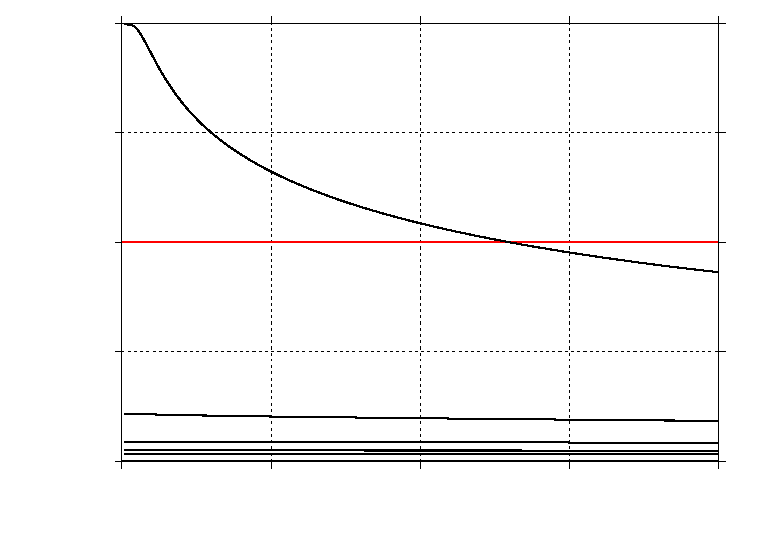
\includegraphics{Figures/TCeigenvalues/TCeigen}}%
    \gplfronttext
  \end{picture}%
\endgroup
  
\caption{In black: The five largest eigenvalues of $L$ plotted as a function of $T$. We see, that the largest eigenvalue intersects 1 (the red line) at one well defined temperature. Parameters: $(n_Ba_{B}^3)^{1/3} = 0.01, (n_Ba_{BF}^3)^{1/3} = 0.1, \frac{m_B}{m_F} = 7/40, \frac{n_F}{n_B^{1/3}} = 0.215$. }
\label{fig.TCeigenvalues}  
\end{center}    
\end{figure}


In figure \ref{fig.TCrB} we see the dependency of $T_c$ on the Bose gas parameter $(n_Ba_B^3)^{1/3}$. We observe a simple monotonic decrease with increasing gas parameter. Physically this can be understood in the following way. When $(n_Ba_B^3)^{1/3}$ is increased for $\frac{n_F}{n_B^{1/3}}$ fixed, the BEC coherence length $k_F\xi = \sqrt{ \frac{\pi}{ 8(n_Ba_B^3)^{1/3} } }\frac{ n_F }{ n_B^{1/3} }$ decreases. The coherence length is the range of the interaction in real space: $\tilde{V}_{\text{ind}} \propto \frac{ \text{e}^{ -\sqrt{2}|x|/\xi } } {|x|}$. Therefore the interaction range is decreased, when we increase $(n_Ba_B^3)^{1/3}$, and so it is physically reasonable, that the critical temperature goes down with increasing $(n_Ba_B^3)^{1/3}$. Notice, that for $(n_Ba_{B}^3)^{1/3} = 0.01$ we recover the critical temperature found in the above: $T_c \approx 0.130 T_F$. 

\begin{figure} 
\begin{center}  
% GNUPLOT: LaTeX picture with Postscript
\begingroup
  \makeatletter
  \providecommand\color[2][]{%
    \GenericError{(gnuplot) \space\space\space\@spaces}{%
      Package color not loaded in conjunction with
      terminal option `colourtext'%
    }{See the gnuplot documentation for explanation.%
    }{Either use 'blacktext' in gnuplot or load the package
      color.sty in LaTeX.}%
    \renewcommand\color[2][]{}%
  }%
  \providecommand\includegraphics[2][]{%
    \GenericError{(gnuplot) \space\space\space\@spaces}{%
      Package graphicx or graphics not loaded%
    }{See the gnuplot documentation for explanation.%
    }{The gnuplot epslatex terminal needs graphicx.sty or graphics.sty.}%
    \renewcommand\includegraphics[2][]{}%
  }%
  \providecommand\rotatebox[2]{#2}%
  \@ifundefined{ifGPcolor}{%
    \newif\ifGPcolor
    \GPcolorfalse
  }{}%
  \@ifundefined{ifGPblacktext}{%
    \newif\ifGPblacktext
    \GPblacktexttrue
  }{}%
  % define a \g@addto@macro without @ in the name:
  \let\gplgaddtomacro\g@addto@macro
  % define empty templates for all commands taking text:
  \gdef\gplbacktext{}%
  \gdef\gplfronttext{}%
  \makeatother
  \ifGPblacktext
    % no textcolor at all
    \def\colorrgb#1{}%
    \def\colorgray#1{}%
  \else
    % gray or color?
    \ifGPcolor
      \def\colorrgb#1{\color[rgb]{#1}}%
      \def\colorgray#1{\color[gray]{#1}}%
      \expandafter\def\csname LTw\endcsname{\color{white}}%
      \expandafter\def\csname LTb\endcsname{\color{black}}%
      \expandafter\def\csname LTa\endcsname{\color{black}}%
      \expandafter\def\csname LT0\endcsname{\color[rgb]{1,0,0}}%
      \expandafter\def\csname LT1\endcsname{\color[rgb]{0,1,0}}%
      \expandafter\def\csname LT2\endcsname{\color[rgb]{0,0,1}}%
      \expandafter\def\csname LT3\endcsname{\color[rgb]{1,0,1}}%
      \expandafter\def\csname LT4\endcsname{\color[rgb]{0,1,1}}%
      \expandafter\def\csname LT5\endcsname{\color[rgb]{1,1,0}}%
      \expandafter\def\csname LT6\endcsname{\color[rgb]{0,0,0}}%
      \expandafter\def\csname LT7\endcsname{\color[rgb]{1,0.3,0}}%
      \expandafter\def\csname LT8\endcsname{\color[rgb]{0.5,0.5,0.5}}%
    \else
      % gray
      \def\colorrgb#1{\color{black}}%
      \def\colorgray#1{\color[gray]{#1}}%
      \expandafter\def\csname LTw\endcsname{\color{white}}%
      \expandafter\def\csname LTb\endcsname{\color{black}}%
      \expandafter\def\csname LTa\endcsname{\color{black}}%
      \expandafter\def\csname LT0\endcsname{\color{black}}%
      \expandafter\def\csname LT1\endcsname{\color{black}}%
      \expandafter\def\csname LT2\endcsname{\color{black}}%
      \expandafter\def\csname LT3\endcsname{\color{black}}%
      \expandafter\def\csname LT4\endcsname{\color{black}}%
      \expandafter\def\csname LT5\endcsname{\color{black}}%
      \expandafter\def\csname LT6\endcsname{\color{black}}%
      \expandafter\def\csname LT7\endcsname{\color{black}}%
      \expandafter\def\csname LT8\endcsname{\color{black}}%
    \fi
  \fi
    \setlength{\unitlength}{0.0500bp}%
    \ifx\gptboxheight\undefined%
      \newlength{\gptboxheight}%
      \newlength{\gptboxwidth}%
      \newsavebox{\gptboxtext}%
    \fi%
    \setlength{\fboxrule}{0.5pt}%
    \setlength{\fboxsep}{1pt}%
\begin{picture}(7200.00,5040.00)%
    \gplgaddtomacro\gplbacktext{%
      \csname LTb\endcsname%
      \put(946,767){\makebox(0,0)[r]{\strut{}$0$}}%
      \csname LTb\endcsname%
      \put(946,1609){\makebox(0,0)[r]{\strut{}$0.05$}}%
      \csname LTb\endcsname%
      \put(946,2451){\makebox(0,0)[r]{\strut{}$0.1$}}%
      \csname LTb\endcsname%
      \put(946,3292){\makebox(0,0)[r]{\strut{}$0.15$}}%
      \csname LTb\endcsname%
      \put(946,4134){\makebox(0,0)[r]{\strut{}$0.2$}}%
      \csname LTb\endcsname%
      \put(946,4976){\makebox(0,0)[r]{\strut{}$0.25$}}%
      \csname LTb\endcsname%
      \put(1141,484){\makebox(0,0){\strut{}$0.005$}}%
      \csname LTb\endcsname%
      \put(2261,484){\makebox(0,0){\strut{}$0.01$}}%
      \csname LTb\endcsname%
      \put(3381,484){\makebox(0,0){\strut{}$0.015$}}%
      \csname LTb\endcsname%
      \put(4500,484){\makebox(0,0){\strut{}$0.02$}}%
      \csname LTb\endcsname%
      \put(5620,484){\makebox(0,0){\strut{}$0.025$}}%
      \csname LTb\endcsname%
      \put(6740,484){\makebox(0,0){\strut{}$0.03$}}%
    }%
    \gplgaddtomacro\gplfronttext{%
      \csname LTb\endcsname%
      \put(176,2871){\rotatebox{-270}{\makebox(0,0){\strut{}$(n_Ba_B^3)^{1/3}$}}}%
      \put(3940,154){\makebox(0,0){\strut{}$T/T_F$}}%
    }%
    \gplbacktext
    \put(0,0){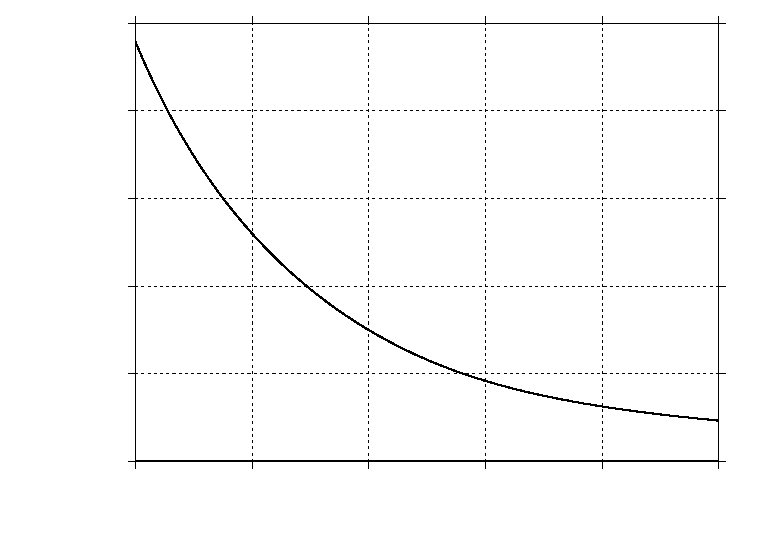
\includegraphics{Figures/TCrB/TCrB}}%
    \gplfronttext
  \end{picture}%
\endgroup
  
\caption{The critical temperatur $T_c$ is plotted as a function of the Bose gas parameter $(n_Ba_B^3)^{1/3}$. We observe a simple monotonic decrease with increasing gas parameter. Other parameters: $(n_Ba_{BF}^3)^{1/3} = 0.1, \frac{m_B}{m_F} = 7/40, \frac{n_F}{n_B^{1/3}} = 0.215$. }  
\label{fig.TCrB}  
\end{center}    
\end{figure}

In figure \ref{fig.TCrBF} we see the dependency of $T_c$ on the Bose-\textit{Fermi} gas parameter $(n_Ba_{BF}^3)^{1/3}$. We observe an increase of $T_c$ with $(n_Ba_{BF}^3)^{1/3}$. This stems from the fact, that a higher value of the Bose-Fermi gas parameter gives a higher interaction strength between the fermions. The system at hand therefore shares one of the key features with the s-wave BCS-theory: any nonzero attractive interaction between the fermions leads to a superfluid phase. 

\begin{figure} 
\begin{center}  
% GNUPLOT: LaTeX picture with Postscript
\begingroup
  \makeatletter
  \providecommand\color[2][]{%
    \GenericError{(gnuplot) \space\space\space\@spaces}{%
      Package color not loaded in conjunction with
      terminal option `colourtext'%
    }{See the gnuplot documentation for explanation.%
    }{Either use 'blacktext' in gnuplot or load the package
      color.sty in LaTeX.}%
    \renewcommand\color[2][]{}%
  }%
  \providecommand\includegraphics[2][]{%
    \GenericError{(gnuplot) \space\space\space\@spaces}{%
      Package graphicx or graphics not loaded%
    }{See the gnuplot documentation for explanation.%
    }{The gnuplot epslatex terminal needs graphicx.sty or graphics.sty.}%
    \renewcommand\includegraphics[2][]{}%
  }%
  \providecommand\rotatebox[2]{#2}%
  \@ifundefined{ifGPcolor}{%
    \newif\ifGPcolor
    \GPcolorfalse
  }{}%
  \@ifundefined{ifGPblacktext}{%
    \newif\ifGPblacktext
    \GPblacktexttrue
  }{}%
  % define a \g@addto@macro without @ in the name:
  \let\gplgaddtomacro\g@addto@macro
  % define empty templates for all commands taking text:
  \gdef\gplbacktext{}%
  \gdef\gplfronttext{}%
  \makeatother
  \ifGPblacktext
    % no textcolor at all
    \def\colorrgb#1{}%
    \def\colorgray#1{}%
  \else
    % gray or color?
    \ifGPcolor
      \def\colorrgb#1{\color[rgb]{#1}}%
      \def\colorgray#1{\color[gray]{#1}}%
      \expandafter\def\csname LTw\endcsname{\color{white}}%
      \expandafter\def\csname LTb\endcsname{\color{black}}%
      \expandafter\def\csname LTa\endcsname{\color{black}}%
      \expandafter\def\csname LT0\endcsname{\color[rgb]{1,0,0}}%
      \expandafter\def\csname LT1\endcsname{\color[rgb]{0,1,0}}%
      \expandafter\def\csname LT2\endcsname{\color[rgb]{0,0,1}}%
      \expandafter\def\csname LT3\endcsname{\color[rgb]{1,0,1}}%
      \expandafter\def\csname LT4\endcsname{\color[rgb]{0,1,1}}%
      \expandafter\def\csname LT5\endcsname{\color[rgb]{1,1,0}}%
      \expandafter\def\csname LT6\endcsname{\color[rgb]{0,0,0}}%
      \expandafter\def\csname LT7\endcsname{\color[rgb]{1,0.3,0}}%
      \expandafter\def\csname LT8\endcsname{\color[rgb]{0.5,0.5,0.5}}%
    \else
      % gray
      \def\colorrgb#1{\color{black}}%
      \def\colorgray#1{\color[gray]{#1}}%
      \expandafter\def\csname LTw\endcsname{\color{white}}%
      \expandafter\def\csname LTb\endcsname{\color{black}}%
      \expandafter\def\csname LTa\endcsname{\color{black}}%
      \expandafter\def\csname LT0\endcsname{\color{black}}%
      \expandafter\def\csname LT1\endcsname{\color{black}}%
      \expandafter\def\csname LT2\endcsname{\color{black}}%
      \expandafter\def\csname LT3\endcsname{\color{black}}%
      \expandafter\def\csname LT4\endcsname{\color{black}}%
      \expandafter\def\csname LT5\endcsname{\color{black}}%
      \expandafter\def\csname LT6\endcsname{\color{black}}%
      \expandafter\def\csname LT7\endcsname{\color{black}}%
      \expandafter\def\csname LT8\endcsname{\color{black}}%
    \fi
  \fi
    \setlength{\unitlength}{0.0500bp}%
    \ifx\gptboxheight\undefined%
      \newlength{\gptboxheight}%
      \newlength{\gptboxwidth}%
      \newsavebox{\gptboxtext}%
    \fi%
    \setlength{\fboxrule}{0.5pt}%
    \setlength{\fboxsep}{1pt}%
\begin{picture}(7200.00,5040.00)%
    \gplgaddtomacro\gplbacktext{%
      \csname LTb\endcsname%
      \put(946,767){\makebox(0,0)[r]{\strut{}$0$}}%
      \csname LTb\endcsname%
      \put(946,1415){\makebox(0,0)[r]{\strut{}$0.02$}}%
      \csname LTb\endcsname%
      \put(946,2062){\makebox(0,0)[r]{\strut{}$0.04$}}%
      \csname LTb\endcsname%
      \put(946,2710){\makebox(0,0)[r]{\strut{}$0.06$}}%
      \csname LTb\endcsname%
      \put(946,3357){\makebox(0,0)[r]{\strut{}$0.08$}}%
      \csname LTb\endcsname%
      \put(946,4005){\makebox(0,0)[r]{\strut{}$0.1$}}%
      \csname LTb\endcsname%
      \put(946,4652){\makebox(0,0)[r]{\strut{}$0.12$}}%
      \csname LTb\endcsname%
      \put(1141,484){\makebox(0,0){\strut{}$0$}}%
      \csname LTb\endcsname%
      \put(2261,484){\makebox(0,0){\strut{}$0.02$}}%
      \csname LTb\endcsname%
      \put(3381,484){\makebox(0,0){\strut{}$0.04$}}%
      \csname LTb\endcsname%
      \put(4500,484){\makebox(0,0){\strut{}$0.06$}}%
      \csname LTb\endcsname%
      \put(5620,484){\makebox(0,0){\strut{}$0.08$}}%
      \csname LTb\endcsname%
      \put(6740,484){\makebox(0,0){\strut{}$0.1$}}%
    }%
    \gplgaddtomacro\gplfronttext{%
      \csname LTb\endcsname%
      \put(176,2871){\rotatebox{-270}{\makebox(0,0){\strut{}$T_c/T_F$}}}%
      \put(3940,154){\makebox(0,0){\strut{}$(n_Ba_{BF}^3)^{1/3}$}}%
    }%
    \gplbacktext
    \put(0,0){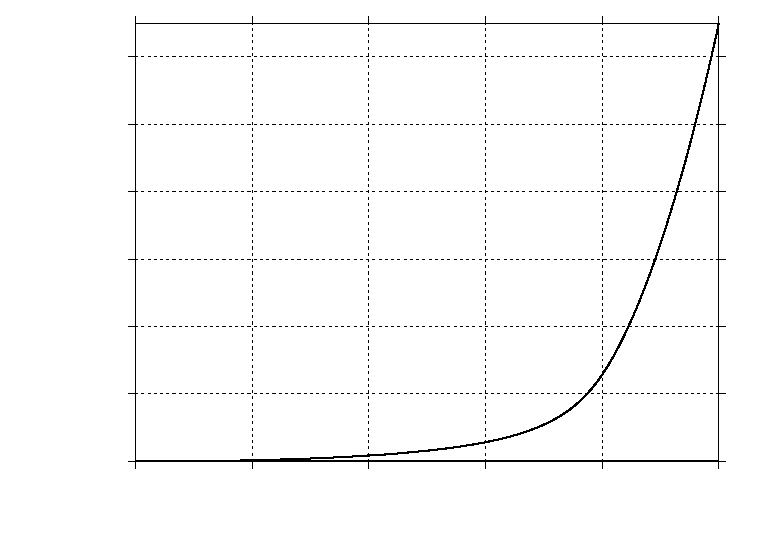
\includegraphics{Figures/TCrBF2/TCrBF}}%
    \gplfronttext
  \end{picture}%
\endgroup
  
\caption{The critical temperatur $T_c$ is plotted as a function of the Bose-Fermi gas parameter $(n_Ba_{BF}^3)^{1/3}$. We see, that for every nonzero induced interaction, there is a superfluid phase for $T\to 0$. Other parameters: $(n_Ba_{B}^3)^{1/3} = 0.01, \frac{m_B}{m_F} = 7/40, \frac{n_F}{n_B^{1/3}} = 0.215$. }  
\label{fig.TCrBF}  
\end{center}    
\end{figure}



 
\chapter{Induced interaction, effective Hamiltonian and topology} 

\label{Chapter7} 

\fancyhead[LO, RE]{Part III. \emph{Kitaev chain}}
\chead{Chapter 7. \emph{Interaction, Hamiltonian \& topology}}
%----------------------------------------------------------------------------------------
In this chapter we derive the effective Hamiltonian for the fermions in a one-dimensional lattice, where the bosons are confined in 1D as well. We start off by going back to the Bose gas and consider the effect of making the gas one-dimensional. See section \ref{sec.1DBosegas}. In section \ref{sec.TightbindingHam.lattice} we introduce the tight-binding Hamiltonian for the lattice fermions. In section \ref{sec.interaction.lattice} we calculate the induced interaction and write up the effective interaction Hamiltonian for the fermions. In section \ref{sec.grandhamiltonian.lattice} we outline the mean field approximation and write down the effective BCS Hamiltonian. Finally, in section \ref{sec.topology.lattice} we discuss the topology of the system and calculate the topological index.

\section{1D Bose gas} \label{sec.1DBosegas}
The reason for confining the bosons in 1D is that the induced interaction becomes longer ranged which is crucial for realising winding numbers larger than 1, as we shall show. In this section we will use Bogoliubov theory to describe the uniform one-dimensional Bose gas. The uniform Bose gas does not show true Bose-Einstein condensation in one dimension. However, in two historical papers by Lieb and Liniger exact solutions for the one-dimensional Bose gas are studied. They find that Bogoliubov theory gives the correct excitation spectrum for a weakly interacting gas \cite{LiebLiniger1, LiebLiniger2}. Further from a more recent paper it is evident that for weak interactions the density-density correlation function is also well-described within Bogoliubov theory \cite{Calabrese}. Since it is exactly the density-density correlation function which is important for our studies, it is justifiable to use Bogoliubov theory.

Going back to equation \eqref{eq.BECHamiltonianrealspace} we have the real space expansion of the Hamiltonian for the bosons:
\begin{equation}
H_{BB} = \int d^3 r \left(\psi_B^\dagger(\mathbf{r})\left[-\frac{\nabla^2}{2m_B}\right]\psi_B(\mathbf{r}) + \frac{g_B}{2}\psi_B^\dagger(\mathbf{r})\psi_B^\dagger(\mathbf{r})\psi_B(\mathbf{r})\psi_B(\mathbf{r})  \right), \nonumber
\end{equation}
The difference from part II is that we now assume that the bosons are trapped along the $x$-axis and that the energy required to be excited in the transverse direction is much larger than the typical energy of the bosons such that the bosons are confined to one dimension. This means that we can make the following expansion for the bosons:
\begin{equation}
\psi_B(x, \mathbf{r}_{\perp}) = \phi_0(\mathbf{r}_{\perp}) \psi_B(x) = \frac{1}{\sqrt{\mathcal{L}}} \sum_k \text{e}^{ikx} \phi_0(\mathbf{r}_{\perp}) b_k, 
\nonumber
\end{equation}
where $\phi_0(\mathbf{r}_\perp) = \frac{1}{\sqrt{\pi}l_t}\text{e}^{-r_{\perp}^2/2l_t^2}$ is the harmonic ground state of the transverse directions with trapping width $l_t$. Inserting this expansion into the quartic interaction part of the Hamiltonian yields:
\begin{equation}
H_{BB}^{\text{int}} = \frac{g_B}{2}\int d^3 r \; \psi_B^\dagger(\mathbf{r})\psi_B^\dagger(\mathbf{r})\psi_B(\mathbf{r})\psi_B(\mathbf{r}) = \frac{g_B}{2\pi l_t^2}\frac{1}{2\mathcal{L}}\sum_{k_1,k_2,q} b^\dagger_{k_1 + q}b^\dagger_{k_2 - q}b_{k_1}b_{k_2}. \nonumber
\end{equation}
We see that this has the exact same form as the momentum space interaction Hamiltonian for the 3D gas contained in equation \eqref{eq.BECHamiltonianmomentumspace}. Further they are equivalent under the identification $g_B \to \frac{g_B}{2\pi l_t^2}$. We could now carry through the Bogoliubov approximation $\psi_B(x) = \sqrt{n_B} + \delta\psi_B(x)$ with $n_B = \frac{N_B}{\mathcal{L}}$ the density of the bosons in the $k = 0$ state and the last term being small relative hereto and containing the $k \neq 0$ terms. The numerics are exactly the same as for the 3D gas, under the above change of $g_B$ and $n_B$. Apart from these differences due to the 1D nature the Bogoliubov theory for the one-dimensional boson gas is qualitatively the same as the three-dimensional one studied in part II. The Green's functions of section \ref{sec.BECGreens} is altered only in the change of $g_B$ and $n_B$. The Bose gas parameter is now $n_Ba_B$ and in turn the coherence length is: $\xi = \frac{l_t}{2\sqrt{n_Ba_B}}$. We are thus ready to calculate the induced interaction for the fermions, mediated by the bosons, once again.

In appendix \ref{Appendix.groundstatedepletion.1DBosegas} we have calculated the ground state depletion of the Bose gas. For Bogoliubov theory to be self-consistent this depletion must be small. From equation \eqref{eq.groundstatedepletion.1Dbosegas} we get that in the thermodynamic limit the depletion diverges $\propto \ln\left(\frac{\sqrt{2}\mathcal{L}}{\pi\xi} \right)$. This emphasizes that Bogoliubov theory is only applicable for a \textit{finite} system in this one-dimensional case and once again illuminates the difficulties of using mean field theory in one dimension, as discussed in section \ref{sec.meanfieldvalidity}. For a finite system the depletion can be controlled to be small by increasing the boson density, $n_B$. 

\section{Tight-binding Hamiltonian} \label{sec.TightbindingHam.lattice}
To get familiar with the relevant energy and length scale we now turn to the tight-binding Hamiltonian.

This time around we trap the fermions along a wire as in the double wire system \textit{and} in a optical lattice. We assume that the trapping frequency, $\omega_t$, for the perpendicular directions to the wire is large with respect to the typical energy of the fermions. This means that the fermions are trapped in the harmonic oscillator ground state like the bosons, i.e. the gaussian $\phi_0(\mathbf{r}_{\perp})$ of width $l_t = \frac{1}{\sqrt{m_F\omega_t}}$. Further, the lattice confinement means that the states can be expanded in terms of well-localised (orthonormal) Wannier states around the lattice points $x_j = jd$, $d$ being the lattice constant. We approximate these states with gaussians $\phi_0(x - x_j)$ of width $l_x$. In this sense, we expand the field operators according to:
\begin{equation}
\psi_F(x, \mathbf{r}_{\perp}) = \sum_j \phi_0(\mathbf{r}_{\perp})\phi_0(x - x_j) c_j, 
\label{eq.fieldexpansionlattice}
\end{equation}
where $c_j$ annihilates a fermion at site $j$. The sum runs over the $N$ lattice sites. The lattice is shown in figure \ref{fig.gasandlattice}. In the next section we will let the lattice site width, $l_x$, go to zero. This strong confinement means that we can safely restrict the Hamiltonian to nearest and next-nearest neighbour hoppings:
\begin{equation}
H_{0} = \frac{1}{2}\sum_{j} \left[- t_1(c^\dagger_{j+1}c_j + c^\dagger_j c_{j + 1}) - t_2(c^\dagger_{j + 2}c_j + c^\dagger_j c_{j + 2}) \right].
\label{eq.Htightbindingrealspace} 
\end{equation}
Here $t_1$ and $t_2$ are the energies associated with nearest and next-nearest neighbour hopping respectively. In a static lattice the next-nearest neighbour hopping is ordinarily several orders of magnitude smaller than $t_1$. However, by shaking the optical lattice one can effectively tune the next-nearest neighbour hopping to be large.
Hence, it is experimentally possible to investigate the entire range of: $t_2 / t_1 \in (0, \infty)$ \cite{Liberto.ShakingOpticalLattice}. 

\begin{figure}
\center
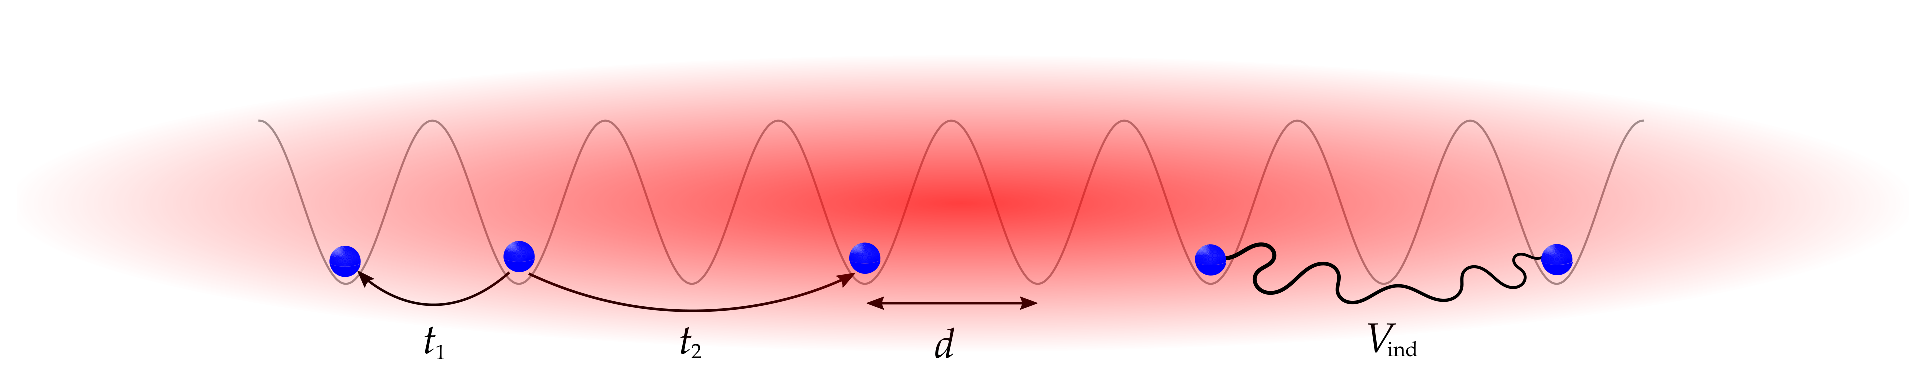
\includegraphics[width=1\columnwidth]{gasandlatticenormalfont.eps}
\caption{In blue: fermions. In red: 1D Bose gas. In grey: optical lattice. The lattice constant is $d$. There is both nearest and next-nearest neighbour hopping, $t_1$ and $t_2$ respectively. The next-nearest neighbour hopping can be tuned to be large by shaking the lattice along its axis. Wiggly line: the contact interaction between the fermions and bosons leads to an induced interaction, $V_{\text{ind}}$, between the fermions. }
\label{fig.gasandlattice}
\end{figure}

We define the momentum space operators through: $c_j = \frac{1}{\sqrt{N}}\sum_{k} c_k \text{e}^{ikx_j}$, where $kd = \frac{2\pi n}{N}$ are the allowed momenta for $n = -\frac{N}{2}, \dots, \frac{N}{2} - 1$ for periodic boundary conditions and $x_j = jd$ the positions of the fermions. Inserting this into the above transforms the Hamiltonian to momentum space:
\begin{equation}
H_{0} = \sum_k \left[ - t_1\cos(kd) - t_2\cos(2kd)\right]c^\dagger_kc_k.
\label{eq.Htightbindingmomentumspace} 
\end{equation}
In this sense, we can already see that going from the homogenous 1D system to the 1D lattice simply corresponds to letting $\frac{k^2}{2m_F} \to - t_1\cos(kd) - t_2\cos(2kd)$. We therefore use $d$ as the unit of length and $t_1$ as the unit of energy. Although this change in dispersion seems trivial, we shall see that it is vital to realise winding numbers larger than 1. 


\section{Effective interaction Hamiltonian} \label{sec.interaction.lattice}
In this section we derive the effective interaction Hamiltonian for the fermions due to their contact interaction with the bosons. We return to the Bose-Fermi interaction Hamiltonian of equation \eqref{eq.HintBF}:
\begin{equation}
H_{BF}^\text{int} = g_{BF}\int d^3 r \; \psi_F^\dagger(\mathbf{r}) \psi_B^\dagger(\mathbf{r})\psi_B(\mathbf{r})\psi_F(\mathbf{r}),
\end{equation} 
Inserting the field expansion of equation \eqref{eq.fieldexpansionlattice} into the interaction Hamiltonian along with the expansion for the bosons, we get:
\begin{equation}
H_{BF}^{\text{int}} = \frac{g_{BF}}{2\pi l_t^2}\frac{1}{\mathcal{L}}\sum_{p_1, p_2, q} c^\dagger_{p_1 - q}b^\dagger_{p_2 + q}b_{p_2}c_{p_1}. \nonumber
\end{equation}
Here we have taken the zero lattice site width limit, $l_x \to 0$, and used that $c_j = \frac{1}{\sqrt{N}}\sum_p \text{e}^{ipx_j}c_p$. The above expression is equivalent to the intrawire interaction for Kitaev wires in the 3D Bose gas by letting $g_{BF} \to \frac{g_{BF}}{2\pi l_t^2}$. As in the double wire system this contact interaction between the fermions and bosons leads to an attractive induced interaction between the fermions which is mediated by the bosons. This is depicted as a wiggly line in figure \ref{fig.gasandlattice}. The calculation of the induced interaction is only altered in the sense that we should not integrate over the perpendicular directions. This is because, the bosons are now also confined to move in one direction. See section \ref{sec.1D3Dinducedinteraction} for the details. Hence, the Fourier transform of the real space interaction is simply given by equation \eqref{eq.V11indXBEC} without the double integration and by letting $g_B \to \frac{g_B}{2\pi l_t^2}, g_{BF} \to \frac{g_{BF}}{2\pi l_t^2}$ and $n_B = \frac{N_B}{\mathcal{L}}$:
\begin{equation}
V_{\text{ind}}(q, i\omega_q) = \left(\frac{g_{BF}}{2\pi l_t^2}\right)^2 \chi_\text{B}(q, i\omega_q), 
\label{eq.VFFmomentumspace.kitaevchain}
\end{equation}
with $\chi_\text{B}(q, i\omega_q) = \frac{q^2}{m_B}\frac{n_B}{(i\omega_q)^2 - E_{B,q}^2}$ the density-density correlation function of the bosons according to Bogoliubov theory. The change of $g_B$ means that the Bogoliubov spectrum $E_{B,q}$ is altered to: $E_{B,q}^2 = \frac{q^2}{2m_B}\left(\frac{q^2}{2m_B} + 2n_B\frac{g_B}{2\pi l_t^2}\right)$.\footnote{Since the coherence length is similarly altered, the spectrum expressed in terms of the coherence length is unaltered.} The real space interaction is obtained by a Fourier transformation of the above. As for the double wire system the frequency dependency is a manifestation of the fact that the bosons move with a finite speed. We will again only study the $\omega_q = 0$ component, whereby we do not take these retardation effects into account. However, we wish to consider long coherence lengths, so it is worth discussing these effects. An upper bound for the momentum of the fermions is provided by the Brillouin zone: $k_F \approx \frac{\pi}{d}$. This means that the relevant speed of the fermions is $v_F = \frac{k_F}{m_F} = \frac{\pi}{m_Fd}$. Letting $g_B \to \frac{g_B}{2\pi l_t^2}$ means that the speed of the bosonic Bogoliubov excitations is: $c_0 = \frac{1}{\sqrt{2}m_B\xi}$. The ratio of the velocities consequently becomes: $\frac{v_F}{c_0} = \sqrt{2}\pi\frac{m_B}{m_F}\frac{\xi}{d}$. The retardation effects are only negligible when $v_F\ll c_0$. This means that either the mass ratio must be unrealistically small, or $\xi \approx d$. Since we wish to consider coherence lengths that are several times the lattice spacing, retardation effects \textit{will} be quantitatively significant. However, we expect that the zero frequency component will give us qualitatively correct results. This is indeed what happens in a 2D system \cite{Jonatan.LatticeFermionsIn3DBEC}. The zero frequency component of the real space interaction is:
\begin{equation}
\tilde{V}_{\text{ind}}(x, 0) = \int \frac{dq}{2\pi} \; \text{e}^{iqx}V_{\text{ind}}(q, 0) = -\frac{n_Bg_{BF}^2m_B}{\pi^2l_t^4}\int \frac{dq}{2\pi} \; \text{e}^{iqx} \frac{1}{q^2 + 2/\xi^2}. \nonumber
\end{equation}
This integration can be performed using Cauchy's residue theorem. The result is:
\begin{equation}
\tilde{V}_{\text{ind}}(j, l, 0) = -\frac{n_Bg_{BF}^2m_B}{2\sqrt{2}\pi^2l_t^4}\xi \cdot \text{e}^{-\frac{\sqrt{2}|x_j - x_l|}{\xi}},
\label{eq.Inducedcinteractionrealspace.kitaevchain}
\end{equation}
where we have put $x = x_j - x_l$, the distance between sites $j$ and $l$. From this it is clear what the effect is of making the boson gas one-dimensional: the induced interaction is no longer of the Yukawa form, it is purely exponential. This is an important difference, since it follows that we can effectively make the interaction over a range of the lattice constant by making the coherence length large enough. The unitless form of this interaction is obtained by dividing by the nearest neighbour hopping $t_1$:
\begin{equation}
\frac{\tilde{V}_{\text{ind}}(j, l, 0)}{t_1} = -G \cdot \text{e}^{-\frac{\sqrt{2}|x_j - x_l|}{\xi}}, \hspace{0.5cm} G = \frac{\sqrt{2}}{\pi^2} \left(\frac{m_F}{m_B} + \frac{m_B}{m_F} + 2\right)\frac{\varepsilon_0}{t_1}\left(\frac{d}{l_t}\right)^3 \frac{(n_Ba_{BF})^2}{n_Bd\sqrt{n_Ba_B}},
\label{eq.Inducedcinteractionrealspaceunitless.kitaevchain} 
\end{equation}
where $G$ is a measure of the strength of the interaction. Here $\varepsilon_0 = \frac{\pi^2}{2m_Fd^2}$ is the energy of a single fermion in an infinite square well of width $d$. We can therefore express the system using the independent variables: $\frac{m_B}{m_F}, n_Bd, \frac{\varepsilon_0}{t_1}, n_B a_{BF}$, and finally the Bose gas parameter: $n_B a_{B}$. In this we assume that we can separately control the hoppings $t_1, t_2$ and the lattice constant $d$. This is the reason for the additional parameter $\frac{\varepsilon_0}{t_1}$. Instead of specifying this large amount of parameters, we will simply set an overall interaction strength $G$ and vary the coherence length, $\xi$. Dropping the $0$ in the induced interaction, we can write the fermion interaction Hamiltonian in the zero frequency limit as:
\begin{equation}
H^{\text{int}}_{FF} = \frac{1}{2}\sum_{j,l} c^\dagger_j c^\dagger_l \tilde{V}_{\text{ind}}(j, l) c_l c_j
\label{eq.Hintrealspace.lattice}
\end{equation}
Using the Fourier decomposition $c_j = \frac{1}{\sqrt{N}}\sum_k \text{e}^{ikx_j}c_k$, we transform this to momentum space:
\begin{align}
H^{\text{int}}_{FF} &= \frac{1}{2N} \sum_{k, q, p} W_{\text{ind}}(k, q, p) c^\dagger_{k + p} c^\dagger_{q - p} c_q c_k, \nonumber \\  
W_{\text{ind}}(k, q, p) &= \frac{1}{2}\sum_{j\neq 0} \left[\cos(px_j) - \cos((k - q + p)x_j) \right]\tilde{V}_{\text{ind}}(0, j). 
\label{eq.Hintmomentumspace.lattice}
\end{align}
We notice that $W_{\text{ind}}(k, q, p)$ is explicitly periodic in the Brillouin zone of width $2\pi / d$. The functional difference between the wire and the lattice is that the momentum space interaction $W_{\text{ind}}(k, q, p)$ is a finite sum of components of the real space interaction $\tilde{V}_{\text{ind}}(0, j)$, not a combination of Fourier transforms. As for the \textit{intra}wire interaction of the double wire system, we have explicitly written the interaction as the sum of a direct term, $\cos(px_j)\tilde{V}_{\text{ind}}(0, j)$ and an exchange term, $ - \cos((k - q + p)x_j)\tilde{V}_{\text{ind}}(0, j)$. See section \ref{sec.HFFint} for the details in the double wire system.ca

\section{Effective Hamiltonian, gap equation and filling fraction} \label{sec.grandhamiltonian.lattice}
The BCS mean field approximation is performed in exactly the same way as for the Kitaev wires. The sum in equation \eqref{eq.Hintmomentumspace.lattice} is truncated to $q = -k$, and the operator $c_kc_{-k}$ is written as its mean plus a deviation. The deviation is then only kept up to first order. See section \ref{sec.meanfieldapproximation} for the details. This means that the Hamiltonian has the exact same structure as for a single wire, but now we use $W_{\text{ind}}(k, k') = W_{\text{ind}}(k, q = -k, p = k' - k)$ of equation \eqref{eq.Hintmomentumspace.lattice} and $\varepsilon_k = - t_1\cos(kd) - t_2\cos(2kd) - \mu$. The system consequently realises the Kitaev chain with next-nearest neighbour hopping included: 
\begin{equation}
H_{FF} = \frac{1}{2}\sum_k \left[\varepsilon_k - \Delta_k \braket {c^\dagger_k c^\dagger_{-k}}\right] + \frac{1}{2}\sum_{k} \begin{bmatrix} c_k^\dagger & c_{-k} \end{bmatrix} \mathcal{H}_{FF,k} \begin{bmatrix} c_k \\ c^\dagger_{-k} \end{bmatrix}, \hspace{0.5cm} \mathcal{H}_{FF,k} = \begin{bmatrix} \varepsilon_k & \Delta_k \\ \Delta^*_k & -\varepsilon_k \end{bmatrix}, 
\label{eq.grandhamiltonian.lattice}
\end{equation}
where the sum over $k$ extends over the Brillouin zone $[-\pi/d, \pi/d )$, and: 
\begin{equation}
\Delta_k = - \frac{1}{N}\sum_{k'} W_{\text{ind}}(k,k')\braket{c_{k'}c_{-k'}}.
\label{eq.pairingpotential.lattice}
\end{equation}ca
The Hamiltonian realises the Kitaev model of section \ref{sec.KitaevModel}. It is therefore readily diagonalised. This yields a dispersion $E_{F,k} = \sqrt{\varepsilon^2_k + |\Delta_k|^2}$. Further using the transformation to the quasiparticle operators, we obtain the gap equation for the pairing potential: 
\begin{align}
\Delta_k &= - \frac{1}{N}\sum_{k'} W_{\text{ind}}(k,k')\frac{\Delta_{k'}}{2E_{F,k'}}\tanh\left[\frac{\beta E_{F,k'}}{2}\right], \nonumber \\
W_{\text{ind}}(k,k') &= \frac{1}{2}\sum_{j\neq 0} \left[\cos((k - k')x_j) - \cos((k + k')x_j) \right]\tilde{V}_{\text{ind}}(0, j).
\label{eq.gapequation.lattice}
\end{align}
So far everything has been analogous to the Kitaev wires. Then, we externally set the number of fermions. In turn the chemical potential adjusted according to the number equation. For the lattice we will externally set the filling fraction $n = N_F / N$ determined by the number equation $N_F = \sum_k \braket{c^\dagger_k c_k}$:
\begin{equation}
n = \frac{N_F}{N} = \frac{1}{N}\sum_k |v_{F,k}|^2 = \frac{1}{2}\left(1 - \frac{1}{N}\sum_k \frac{\varepsilon_k}{E_{F,k}}\tanh\left[\frac{\beta E_{F,k}}{2} \right] \right) 
\label{eq.fillingfraction.lattice}
\end{equation}
which measures how full the lattice is. In turn the chemical potential will again adjust. Since the lattice consists of identical fermions the filling fraction is less than 1: $0 \leq n \leq 1$. A small calculation shows that in the extreme cases $n = 0$ and $n = 1$, the pairing vanishes: $\Delta_k = 0$. The former is easily understood: there is no pairing between the fermions, if there are no fermions present. The latter, $n = 1$, is also physically intuitive: the lattice can only be a superfluid, if there are vacant sites. Else the lattice turns rigid, since the fermions can only hop to vacant sites. In addition to the overall interaction strength, $G$, and the coherence length, $\xi / d$, we thus have to specify the filling, $n$. This gives us essentially only three parameters to vary. 

To have a clearer intuition for the chemical potential we solve for it, for $G = t_2 = T = 0$, i.e. the nearest neighbour tight binding model with no pairing at zero temperature. In this case the above equation can be written simply as:
\begin{equation}
n = \frac{1}{2N}\sum_k \left( 1 - \frac{\varepsilon_k}{|\varepsilon_k|}\right) = \frac{2}{N}\sum_{k > 0, k < k_1}. \nonumber
\end{equation}
Here we have used that the summand is even in $k$, and defined $k_1$ through: $0 = \varepsilon_{k = k_1} = -t_1\cos(k_1d) - \mu$. Further we use that $1 - \frac{\varepsilon_k}{|\varepsilon_k|} = 2$ for $-k_1 < k < k_1$ and $0$ otherwise. The sum can be evaluated when $N \gg 1$. By letting $\sum_k \to \frac{1}{\Delta k}\int dk$ we get:
\begin{equation}
n = \frac{d}{\pi}\int_0^{k_1} dk =  \frac{k_1d}{\pi} = \frac{\cos^{-1}\left(-\frac{\mu}{t_1}\right)}{\pi}. \nonumber
\end{equation}
Here we use $\varepsilon_{k_1} = 0 \Rightarrow k_1d = \cos^{-1}\left(-\frac{\mu}{t_1}\right)$. Hence we get a simple expression for $\mu(n)$ for $N\gg 1$:
\begin{equation}
\mu(n) = -t_1\cos(\pi n), \hspace{0.5cm} G = t_2 = T = 0, N\gg 1. 
\label{eq.mun.T0.G0.t20.lattice}
\end{equation}
We notice that $\mu$ is bounded to lie between $-t_1$ and $t_1$ hitting these for $n = 0$ and $n = 1$ respectively, as it should in the noninteracting $T = 0$ case. More specifically we can understand this cosinusoidal behaviour as follows. The key is the form of kinetic energy $-t_1\cos(kd)$. For small filling only the bottom most points of $-t_1\cos(kd)$ are occupied. The band is flat in this region, so the chemical potential increases slowly with $n$. When we reach $n = 1/2$ the band is linear, and there is a linear relation between $\mu$ and $n$. When the filling becomes very close to one, the band again flattens out and $\mu$ changes very slowly with rising $n$. For $n = 1$ the band is completely full and $\mu = t_1$. The chemical potential is plotted as a function of the filling in figure \ref{fig.mun.t20.Gdepend} of the next chapter. 

\section{Filling fraction symmetry}
\label{sec.fillingfractionsymmetry.breakdown}
In this section we show that the system has a filling fraction symmetry $n \to 1 - n$, when next-nearest neighbour hopping is absent, i.e. $t_2 = 0$. We will also show, how $t_2 \neq 0$ breaks this symmetry. 

For $t_2 = 0$, transforming the filling fraction of equation \eqref{eq.fillingfraction.lattice} to $n' = 1 - n$ we get:
\begin{align}
n' 	&= \frac{1}{2}\left(1 + \frac{1}{N}\sum_k \frac{\varepsilon_k}{E_{F,k}}\tanh\left[\frac{\beta E_{F,k}}{2} \right] \right) = \frac{1}{2}\left(1 + \frac{1}{N}\sum_k \frac{\varepsilon_{k + \pi/d}}{E_{F,k + \pi/d}}\tanh\left[\frac{\beta E_{F,k + \pi/d}}{2} \right] \right) \nonumber \\ 
	&= \frac{1}{2}\left(1 - \frac{1}{N}\sum_k \frac{\varepsilon_{k}(-\mu)}{E_{F,k}(-\mu, \Delta_{k + \pi/d})}\tanh\left[\frac{\beta E_{F,k}(-\mu, \Delta_{k + \pi/d})}{2} \right] \right), \nonumber
\end{align}
where we use that $\varepsilon_{k + \pi / d}( \mu ) = -t_1\cos(kd + \pi) - \mu = - \varepsilon_k(-\mu)$. Further, $E^2_{F,k}(-\mu, \Delta_{k + \pi/d}) = (-t_1\cos(kd)+\mu)^2 + \Delta^2_{k+\pi/d}$. This means that if we come from a system with a solution $n, \mu, \Delta_k$ and change $n \to n' = 1 - n$, then this has the solution $1 - n, -\mu, \Delta_{k+\pi/d}$. It is in this sense, the system has a symmetry in the filling fraction. Specifically this is around $n = 1/2$.\footnote{This must in fact also be checked for consistency with the gap equation \eqref{eq.gapequation.lattice}. This is quite simply and verifies the new solution $\Delta_{k + \pi/d}$. } 

We now show how a next-nearest neighbour hopping $t_2 \neq 0$ break the $n \to 1 - n$ symmetry. The key point above was to use the transformation $k\to k + \pi/d$. Under this transformation now: $\varepsilon_{k + \pi/d} = -t_1\cos(kd + \pi) - t_2\cos(2kd + 2\pi) - \mu = t_1\cos(kd) - t_2\cos(2kd) - \mu = -\varepsilon_k(t_1,-t_2,-\mu)$. Hence, to obtain a symmetry we now also need to transform $t_2 \to -t_2$. It is in this sense the nearest neighbour hopping \textit{breaks} the filling fraction symmetry around $n = 1/2$. 

We emphasize that this filling fraction symmetry is not simply a particle-hole symmetry, $c_i \to c^\dagger_i$. The particle-hole symmetry is always present and corresponds to the transformation: $n \to 1 - n, \mu \to -\mu, t_1 \to -t_1, t_2 \to -t_2$ and  $\Delta_k \to \Delta_k^*$. Hence, it requires a flip in sign of the nearest neighbour hopping, $t_1$, as well and changes the pairing in a different manner.  

\section{Topology} \label{sec.topology.lattice}
We are now ready to show that the proposed model can realise winding numbers larger than 1. We remind ourselves that since the system has a particle-hole symmetry with $C^2 = + \mathbb{I}$ as well as a time reversal symmetry with $T^2 = +\mathbb{I}$, it belongs to Cartan class BDI with a $\mathbb{Z}$ topological index. 

In subsection \ref{subsec.topologicalinvariant.singlewire} we studied the Kitaev single wire. We showed that the $\mathbb{Z}$ topological index is the winding number of a specific mapping. The mapping is defined in the following manner. We write $\mathcal{H}_{FF,k} = \mathbf{h}(k)\cdot \boldsymbol\tau$ with $\boldsymbol\tau = (\tau_1, \tau_2, \tau_3)$ and $\mathbf{h}(k) = (\Delta_k, 0, \epsilon_k)$ for $\Delta_k$ real. The mapping is then given by $\hat{h}(k) = \frac{\mathbf{h}(k)}{|\mathbf{h}(k)|}$ which maps from the Brillouin zone to the unit circle. Since $E_{F,k} = |\mathbf{h}(k)|$ the mapping is well-defined as long as the system has an energy gap. The winding number of this mapping was found in section \ref{subsec.topologicalinvariant.singlewire}. Adjusting for the fact that the Brillouin zone is now $[-\pi/d, \pi/d)$, we get:
\begin{equation}
w = \frac{1}{2\pi}\oint d\theta_k = \frac{1}{2\pi}\int_{-\pi/d}^{\pi/d} dk \frac{\varepsilon_k\partial_k\Delta_k - \Delta_k\partial_k\varepsilon_k}{\varepsilon^2_k + \Delta^2_k} = \frac{1}{\pi}\int_{0}^{\pi/d} dk \frac{\varepsilon_k\partial_k\Delta_k - \Delta_k\partial_k\varepsilon_k}{\varepsilon^2_k + \Delta^2_k}. 
\label{eq.windingnumber.kitaevmodel}
\end{equation} 
In section \ref{sec.2wires_CSinv} we calculated the topological invariant for the Kitaev wires. Then the kinetic energy only had a single pair of Fermi points. Now we wish to generalise this strategy to the case, where $\varepsilon_k$ has several pairs of Fermi points, i.e. several pairs of zeroes. To keep the calculation simple we will assume that there are only up to two pairs of zeroes. We can achieve this by adding next-nearest neighbour hopping, since it corresponds to the addition of the term $-t_2\cos(2kd)$ to $\varepsilon_k$ which makes the dispersion bend downwards towards the Brillouin zone boundary. In figure \ref{fig.dispersions.lattice} we have plotted several possibilities for the dispersion for $t_2 = t_1$ and the resulting pairing. The two pairs of zeros is apparent in the bottom two figures. We denote the zeroes for $k > 0$ as $0 < k_1 < k_2 < \pi / d$.\footnote{One could equivalently use the negative zeroes.} The primitive of the integrand above was also found in section \ref{sec.2wires_CSinv} and is given by:
\begin{equation}
\theta_k(c) = \arctan\left(\frac{\Delta_k}{\varepsilon_k}\right) + c, \nonumber
\end{equation}
where $c$ is some constant. As for the double wire system, $\theta_k(0)$ suffers discontinuities when $\varepsilon_k$ hits zero which must be remedied. Explicitly, we found a discontinuity of $\pm \pi$ depending on the sign of $\Delta_k$ and whether $\varepsilon_k$ approaches zero from negative or positive values. Hence, we can form the continuous primitive:
\begin{equation}
\theta_k = \left\{ \begin{matrix} 
\arctan\left(\frac{\Delta_k}{\varepsilon_k}\right), & 0 < k < k_1, \\
\arctan\left(\frac{\Delta_k}{\varepsilon_k}\right) - \pi\text{sgn}(\Delta_{k_1})\text{sgn}\left(\partial_k\varepsilon_{k = k_1}\right), & k_1 < k < k_2, \\
\arctan\left(\frac{\Delta_k}{\varepsilon_k}\right) - \pi\left(\text{sgn}(\Delta_{k_1})\text{sgn}\left(\partial_k\varepsilon_{k = k_1}\right) + \text{sgn}(\Delta_{k_2})\text{sgn}\left(\partial_k\varepsilon_{k = k_2}\right)\right), & k_2 < k < \pi / d,
  \end{matrix} \right. \nonumber 
\end{equation}
where $\partial_k\varepsilon_{k = k_i}$ denotes the derivative $\partial_k\varepsilon_k$ at $k_i$ and $\text{sgn}$ is the sign function. The integral can now be evaluated using the above primitive:
\begin{equation}
w = \left.\frac{1}{\pi}\theta_k\right|^{\pi / d}_{0} = -\left( \text{sgn}\left(\Delta_{k_1}\partial_k\varepsilon_{k = k_1}\right) + \text{sgn}\left(\Delta_{k_2}\partial_k\varepsilon_{k = k_2}\right) \right). \nonumber
\end{equation}
Here we put the signs together. This formula illustrates the fact that we can flip the sign of the winding number by flipping the overal sign of the pairing, $\Delta_k$. In our analysis we will only consider a single lattice. This means that this overall sign is irrelevant, and we can take the invariant to be the absolute value: $\nu = |w|$.\footnote{If we e.g. considered two lattices in junction, the sign would matter, but in the present context it does not.} In the case of nearest and next-nearest neighbour hopping we hereby see that:
\begin{equation}
\nu = \left\{ \begin{matrix} 	0, 								& \text{no zeroes of } \varepsilon_k, \\
								1, 								& \varepsilon_{k_1} = 0, \\
								\left|\text{sgn}(\Delta_{k_1}\partial_k\varepsilon_{k = k_1}) + \text{sgn}(\Delta_{k_2}\partial_k\varepsilon_{k = k_2})\right|,   & \varepsilon_{k_1} = 0 = \varepsilon_{k_2}.
\end{matrix} \right. \nonumber
\end{equation}
Here we see that for $0$ and $1$ pairs of zeroes of $\varepsilon_k$, the invariant is unambigously also $0$ and $1$ respectively. However, for $2$ pairs of zeroes, the invariant can both be $0$ and $2$. Further, since the slope of $\varepsilon_k$ will have opposite sign at $k_1$ and $k_2$ we see the following two conditions must be satisfied to get a topological invariant $\nu = 2$. First, there must be \textit{two} zeroes of $\varepsilon_k$. Second, the sign of the pairing must be different at these two zeroes. In this manner we have established a general formula for the topological invariant in case of an arbitrary number of pairs of zeroes of $\varepsilon_k$:
\begin{equation}
\nu = \left|\sum_{k_n > 0, \varepsilon_{k_n} = 0} \text{sgn}\left(\Delta_{k_n}\partial_k\varepsilon_{k = k_n}\right)\right|.
\label{eq.topologicalinvariant}
\end{equation} 

\begin{figure}
\begin{center}
% GNUPLOT: LaTeX picture with Postscript
\begingroup
  \makeatletter
  \providecommand\color[2][]{%
    \GenericError{(gnuplot) \space\space\space\@spaces}{%
      Package color not loaded in conjunction with
      terminal option `colourtext'%
    }{See the gnuplot documentation for explanation.%
    }{Either use 'blacktext' in gnuplot or load the package
      color.sty in LaTeX.}%
    \renewcommand\color[2][]{}%
  }%
  \providecommand\includegraphics[2][]{%
    \GenericError{(gnuplot) \space\space\space\@spaces}{%
      Package graphicx or graphics not loaded%
    }{See the gnuplot documentation for explanation.%
    }{The gnuplot epslatex terminal needs graphicx.sty or graphics.sty.}%
    \renewcommand\includegraphics[2][]{}%
  }%
  \providecommand\rotatebox[2]{#2}%
  \@ifundefined{ifGPcolor}{%
    \newif\ifGPcolor
    \GPcolorfalse
  }{}%
  \@ifundefined{ifGPblacktext}{%
    \newif\ifGPblacktext
    \GPblacktexttrue
  }{}%
  % define a \g@addto@macro without @ in the name:
  \let\gplgaddtomacro\g@addto@macro
  % define empty templates for all commands taking text:
  \gdef\gplbacktext{}%
  \gdef\gplfronttext{}%
  \makeatother
  \ifGPblacktext
    % no textcolor at all
    \def\colorrgb#1{}%
    \def\colorgray#1{}%
  \else
    % gray or color?
    \ifGPcolor
      \def\colorrgb#1{\color[rgb]{#1}}%
      \def\colorgray#1{\color[gray]{#1}}%
      \expandafter\def\csname LTw\endcsname{\color{white}}%
      \expandafter\def\csname LTb\endcsname{\color{black}}%
      \expandafter\def\csname LTa\endcsname{\color{black}}%
      \expandafter\def\csname LT0\endcsname{\color[rgb]{1,0,0}}%
      \expandafter\def\csname LT1\endcsname{\color[rgb]{0,1,0}}%
      \expandafter\def\csname LT2\endcsname{\color[rgb]{0,0,1}}%
      \expandafter\def\csname LT3\endcsname{\color[rgb]{1,0,1}}%
      \expandafter\def\csname LT4\endcsname{\color[rgb]{0,1,1}}%
      \expandafter\def\csname LT5\endcsname{\color[rgb]{1,1,0}}%
      \expandafter\def\csname LT6\endcsname{\color[rgb]{0,0,0}}%
      \expandafter\def\csname LT7\endcsname{\color[rgb]{1,0.3,0}}%
      \expandafter\def\csname LT8\endcsname{\color[rgb]{0.5,0.5,0.5}}%
    \else
      % gray
      \def\colorrgb#1{\color{black}}%
      \def\colorgray#1{\color[gray]{#1}}%
      \expandafter\def\csname LTw\endcsname{\color{white}}%
      \expandafter\def\csname LTb\endcsname{\color{black}}%
      \expandafter\def\csname LTa\endcsname{\color{black}}%
      \expandafter\def\csname LT0\endcsname{\color{black}}%
      \expandafter\def\csname LT1\endcsname{\color{black}}%
      \expandafter\def\csname LT2\endcsname{\color{black}}%
      \expandafter\def\csname LT3\endcsname{\color{black}}%
      \expandafter\def\csname LT4\endcsname{\color{black}}%
      \expandafter\def\csname LT5\endcsname{\color{black}}%
      \expandafter\def\csname LT6\endcsname{\color{black}}%
      \expandafter\def\csname LT7\endcsname{\color{black}}%
      \expandafter\def\csname LT8\endcsname{\color{black}}%
    \fi
  \fi
    \setlength{\unitlength}{0.0500bp}%
    \ifx\gptboxheight\undefined%
      \newlength{\gptboxheight}%
      \newlength{\gptboxwidth}%
      \newsavebox{\gptboxtext}%
    \fi%
    \setlength{\fboxrule}{0.5pt}%
    \setlength{\fboxsep}{1pt}%
\begin{picture}(7200.00,5040.00)%
    \gplgaddtomacro\gplbacktext{%
      \csname LTb\endcsname%
      \put(165,2646){\makebox(0,0)[r]{\strut{}$-3$}}%
      \put(165,2961){\makebox(0,0)[r]{\strut{}$-2$}}%
      \put(165,3276){\makebox(0,0)[r]{\strut{}$-1$}}%
      \put(165,3591){\makebox(0,0)[r]{\strut{}$0$}}%
      \put(165,3905){\makebox(0,0)[r]{\strut{}$1$}}%
      \put(165,4220){\makebox(0,0)[r]{\strut{}$2$}}%
      \put(165,4535){\makebox(0,0)[r]{\strut{}$3$}}%
      \put(429,2363){\makebox(0,0){\strut{} }}%
      \put(916,2363){\makebox(0,0){\strut{} }}%
      \put(1403,2363){\makebox(0,0){\strut{} }}%
      \put(1890,2363){\makebox(0,0){\strut{} }}%
      \put(2376,2363){\makebox(0,0){\strut{} }}%
      \put(2863,2363){\makebox(0,0){\strut{} }}%
      \put(3350,2363){\makebox(0,0){\strut{} }}%
    }%
    \gplgaddtomacro\gplfronttext{%
      \csname LTb\endcsname%
      \put(-341,3590){\rotatebox{-270}{\makebox(0,0){\strut{}$\varepsilon_k, \Delta_k$}}}%
      \put(833,4378){\makebox(0,0){\strut{}$\nu = 1$}}%
    }%
    \gplgaddtomacro\gplbacktext{%
      \csname LTb\endcsname%
      \put(3584,2646){\makebox(0,0)[r]{\strut{} }}%
      \put(3584,2961){\makebox(0,0)[r]{\strut{} }}%
      \put(3584,3276){\makebox(0,0)[r]{\strut{} }}%
      \put(3584,3591){\makebox(0,0)[r]{\strut{} }}%
      \put(3584,3905){\makebox(0,0)[r]{\strut{} }}%
      \put(3584,4220){\makebox(0,0)[r]{\strut{} }}%
      \put(3584,4535){\makebox(0,0)[r]{\strut{} }}%
      \put(3848,2363){\makebox(0,0){\strut{} }}%
      \put(4335,2363){\makebox(0,0){\strut{} }}%
      \put(4822,2363){\makebox(0,0){\strut{} }}%
      \put(5309,2363){\makebox(0,0){\strut{} }}%
      \put(5796,2363){\makebox(0,0){\strut{} }}%
      \put(6283,2363){\makebox(0,0){\strut{} }}%
      \put(6770,2363){\makebox(0,0){\strut{} }}%
    }%
    \gplgaddtomacro\gplfronttext{%
      \csname LTb\endcsname%
      \put(4253,4378){\makebox(0,0){\strut{}$\nu = 1$}}%
    }%
    \gplgaddtomacro\gplbacktext{%
      \csname LTb\endcsname%
      \put(165,504){\makebox(0,0)[r]{\strut{}$-3$}}%
      \put(165,819){\makebox(0,0)[r]{\strut{}$-2$}}%
      \put(165,1134){\makebox(0,0)[r]{\strut{}$-1$}}%
      \put(165,1449){\makebox(0,0)[r]{\strut{}$0$}}%
      \put(165,1763){\makebox(0,0)[r]{\strut{}$1$}}%
      \put(165,2078){\makebox(0,0)[r]{\strut{}$2$}}%
      \put(165,2393){\makebox(0,0)[r]{\strut{}$3$}}%
      \put(429,221){\makebox(0,0){\strut{}$-3$}}%
      \put(916,221){\makebox(0,0){\strut{}$-2$}}%
      \put(1403,221){\makebox(0,0){\strut{}$-1$}}%
      \put(1890,221){\makebox(0,0){\strut{}$0$}}%
      \put(2376,221){\makebox(0,0){\strut{}$1$}}%
      \put(2863,221){\makebox(0,0){\strut{}$2$}}%
      \put(3350,221){\makebox(0,0){\strut{}$3$}}%
    }%
    \gplgaddtomacro\gplfronttext{%
      \csname LTb\endcsname%
      \put(-209,1448){\rotatebox{-270}{\makebox(0,0){\strut{}$\varepsilon_k, \Delta_k$}}}%
      \put(1889,-109){\makebox(0,0){\strut{}$kd$}}%
      \put(833,2236){\makebox(0,0){\strut{}$\nu = 0$}}%
    }%
    \gplgaddtomacro\gplbacktext{%
      \csname LTb\endcsname%
      \put(3584,504){\makebox(0,0)[r]{\strut{} }}%
      \put(3584,819){\makebox(0,0)[r]{\strut{} }}%
      \put(3584,1134){\makebox(0,0)[r]{\strut{} }}%
      \put(3584,1449){\makebox(0,0)[r]{\strut{} }}%
      \put(3584,1763){\makebox(0,0)[r]{\strut{} }}%
      \put(3584,2078){\makebox(0,0)[r]{\strut{} }}%
      \put(3584,2393){\makebox(0,0)[r]{\strut{} }}%
      \put(3848,221){\makebox(0,0){\strut{}$-3$}}%
      \put(4335,221){\makebox(0,0){\strut{}$-2$}}%
      \put(4822,221){\makebox(0,0){\strut{}$-1$}}%
      \put(5309,221){\makebox(0,0){\strut{}$0$}}%
      \put(5796,221){\makebox(0,0){\strut{}$1$}}%
      \put(6283,221){\makebox(0,0){\strut{}$2$}}%
      \put(6770,221){\makebox(0,0){\strut{}$3$}}%
    }%
    \gplgaddtomacro\gplfronttext{%
      \csname LTb\endcsname%
      \put(5309,-109){\makebox(0,0){\strut{}$kd$}}%
      \put(4253,2236){\makebox(0,0){\strut{}$\nu = 2$}}%
    }%
    \gplbacktext
    \put(0,0){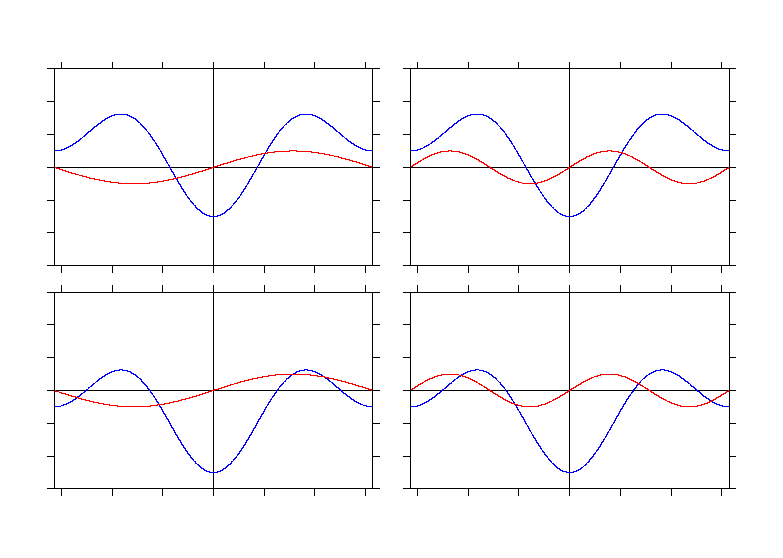
\includegraphics{Figures/Lattice.singlewire/dispersion/kdepend}}%
    \gplfronttext
  \end{picture}%
\endgroup

\caption{In blue: kinetic energy relative to chemical potential, $\varepsilon_k$. In red: pairing $\Delta_k$. Both in units of $t_1$ as a function of $kd$. Top row: $\mu = -0.5 t_1$. Bottom row: $\mu = 0.5 t_1$. Left column: $\Delta_k = \frac{t_1}{2}\sin(kd)$. Right column: $\Delta_k = \frac{t_1}{2}\sin(2kd)$. The bottom right figure is the only one that exhibits $\nu = 2$, since we both need two zeroes for $k >0$ of $\varepsilon_k$ and a change in sign of $\Delta_k$ in-between these zeroes. For all figures we have set $t_2 = t_1$. }
\label{fig.dispersions.lattice}
\end{center}
\end{figure}

Hence, for every positive zero, $k_n$, of $\varepsilon_k$ there is a contribution to the invariant of $\text{sgn}\left(\Delta_{k_n}\partial_k\varepsilon_{k = k_n}\right)$. For the sake of clarity let us see, how we use this formula on the examples given in figure \ref{fig.dispersions.lattice}. Here we assume the pairing, shown in red, is either proportional to $\sin(kd)$ or $\sin(2kd)$, respectively the left and right column. The kinetic energy dispersion is shown in blue for two values of the chemical potential $\mu / t_1 = -1/2$ and $\mu / t_1 = 1/2$, top and bottom row respectively. The required \textit{two} zeroes of $\varepsilon_k$ for $\nu = 2$ is achieved in the bottom two figures. It is clear from the figure that this is equivalent to a high filling fraction, since much of $\varepsilon_k$ must be negative. Further, we need the pairing to change sign in between the two zeroes of $\varepsilon_k$. Hence, a $\sin(2kd)$-like pairing is needed as well. 

This section explicitly demonstrates that the 1D tight-binding model with next-nearest neighbour hopping opens up the possibility to realise winding numbers larger than 1. In the next chapter, we will solve the gap and number equations self-consistently to see if this can actually be achieved. We will see that we need a long coherence length, since the $\sin(lkd)$ term of $\Delta_k$ is connected to pairing to the $l$'th neighbour. We will expand on this analysis in the following chapter, where we explicitly find the pairing using equation \eqref{eq.gapequation.lattice}.

 

\part{Two wires}

\newpage

\chapter{Numerical analysis} % Main chapter title

\label{Chapter8} 

\fancyhead[LO, RE]{Part III. \emph{Kitaev chain}}
\chead{Chapter 8. \emph{Numerical analysis}} % This is for the header on each page - perhaps a shortened title
%----------------------------------------------------------------------------------------
In this chapter we present a numerical analysis for the Kitaev chain in the one-dimensional Bose gas. Our focus is on the topological properties of the ground state of the system which is characterised by the winding number. In section \ref{sec.onlyNN} we briefly investigate the nearest neighbour hopping only, i.e. $t_2 = 0$. In section \ref{sec.NNNincluded} we include the next-nearest neighbour hopping and study the effect of introducing this parameter. 
 
\section{Only nearest neighbour hopping} \label{sec.onlyNN}
We numerically study the system as a function of two parameters: the BEC coherence length, $\xi$, and the filling fraction $n = N_F/N$. We keep the interaction strength, $G$, constant. The phase diagrams are produced in the following manner. For each value of $\xi$ we compute the effective interaction using equation \eqref{eq.gapequation.lattice}. Then for each value of $n$ we come with an initial guess for the pairing. We use $\sin(kd)$, since this is the expected behaviour. Finally, we use equations \eqref{eq.gapequation.lattice} and \eqref{eq.fillingfraction.lattice} to solve for the pairing and chemical potentials in a self-consistent manner at zero temperature. This is done in precisely the same way as for double wire system. This procedure to find a self-consistent solution is then repeated for varying filling fractions $0 \leq n \leq 1$ and BEC coherence lengths. 

The result of the analysis for $G = 4$ and $G = 8$ is shown in figure \ref{fig.phasediagram.t20}, where we plot the winding number, $\nu$, as a function of the filling fraction and the BEC coherence length. We notice that the phase diagrams are symmetrical around $n = 1/2$. In addition a higher interaction strength leads to a narrower window of the topologically nontrivial phase of $\nu = 1$ shown in red. Finally, as the coherence length grows, the topological nontrivial phase narrows. We can understand these three effects in the following manner. 

\begin{figure}
\begin{center}
% GNUPLOT: LaTeX picture with Postscript
\begingroup
  \makeatletter
  \providecommand\color[2][]{%
    \GenericError{(gnuplot) \space\space\space\@spaces}{%
      Package color not loaded in conjunction with
      terminal option `colourtext'%
    }{See the gnuplot documentation for explanation.%
    }{Either use 'blacktext' in gnuplot or load the package
      color.sty in LaTeX.}%
    \renewcommand\color[2][]{}%
  }%
  \providecommand\includegraphics[2][]{%
    \GenericError{(gnuplot) \space\space\space\@spaces}{%
      Package graphicx or graphics not loaded%
    }{See the gnuplot documentation for explanation.%
    }{The gnuplot epslatex terminal needs graphicx.sty or graphics.sty.}%
    \renewcommand\includegraphics[2][]{}%
  }%
  \providecommand\rotatebox[2]{#2}%
  \@ifundefined{ifGPcolor}{%
    \newif\ifGPcolor
    \GPcolorfalse
  }{}%
  \@ifundefined{ifGPblacktext}{%
    \newif\ifGPblacktext
    \GPblacktexttrue
  }{}%
  % define a \g@addto@macro without @ in the name:
  \let\gplgaddtomacro\g@addto@macro
  % define empty templates for all commands taking text:
  \gdef\gplbacktext{}%
  \gdef\gplfronttext{}%
  \makeatother
  \ifGPblacktext
    % no textcolor at all
    \def\colorrgb#1{}%
    \def\colorgray#1{}%
  \else
    % gray or color?
    \ifGPcolor
      \def\colorrgb#1{\color[rgb]{#1}}%
      \def\colorgray#1{\color[gray]{#1}}%
      \expandafter\def\csname LTw\endcsname{\color{white}}%
      \expandafter\def\csname LTb\endcsname{\color{black}}%
      \expandafter\def\csname LTa\endcsname{\color{black}}%
      \expandafter\def\csname LT0\endcsname{\color[rgb]{1,0,0}}%
      \expandafter\def\csname LT1\endcsname{\color[rgb]{0,1,0}}%
      \expandafter\def\csname LT2\endcsname{\color[rgb]{0,0,1}}%
      \expandafter\def\csname LT3\endcsname{\color[rgb]{1,0,1}}%
      \expandafter\def\csname LT4\endcsname{\color[rgb]{0,1,1}}%
      \expandafter\def\csname LT5\endcsname{\color[rgb]{1,1,0}}%
      \expandafter\def\csname LT6\endcsname{\color[rgb]{0,0,0}}%
      \expandafter\def\csname LT7\endcsname{\color[rgb]{1,0.3,0}}%
      \expandafter\def\csname LT8\endcsname{\color[rgb]{0.5,0.5,0.5}}%
    \else
      % gray
      \def\colorrgb#1{\color{black}}%
      \def\colorgray#1{\color[gray]{#1}}%
      \expandafter\def\csname LTw\endcsname{\color{white}}%
      \expandafter\def\csname LTb\endcsname{\color{black}}%
      \expandafter\def\csname LTa\endcsname{\color{black}}%
      \expandafter\def\csname LT0\endcsname{\color{black}}%
      \expandafter\def\csname LT1\endcsname{\color{black}}%
      \expandafter\def\csname LT2\endcsname{\color{black}}%
      \expandafter\def\csname LT3\endcsname{\color{black}}%
      \expandafter\def\csname LT4\endcsname{\color{black}}%
      \expandafter\def\csname LT5\endcsname{\color{black}}%
      \expandafter\def\csname LT6\endcsname{\color{black}}%
      \expandafter\def\csname LT7\endcsname{\color{black}}%
      \expandafter\def\csname LT8\endcsname{\color{black}}%
    \fi
  \fi
    \setlength{\unitlength}{0.0500bp}%
    \ifx\gptboxheight\undefined%
      \newlength{\gptboxheight}%
      \newlength{\gptboxwidth}%
      \newsavebox{\gptboxtext}%
    \fi%
    \setlength{\fboxrule}{0.5pt}%
    \setlength{\fboxsep}{1pt}%
\begin{picture}(7200.00,5040.00)%
    \gplgaddtomacro\gplbacktext{%
      \csname LTb\endcsname%
      \put(165,756){\makebox(0,0)[r]{\strut{}$1$}}%
      \put(165,1386){\makebox(0,0)[r]{\strut{}$2$}}%
      \put(165,2016){\makebox(0,0)[r]{\strut{}$3$}}%
      \put(165,2646){\makebox(0,0)[r]{\strut{}$4$}}%
      \put(165,3275){\makebox(0,0)[r]{\strut{}$5$}}%
      \put(165,3905){\makebox(0,0)[r]{\strut{}$6$}}%
      \put(165,4535){\makebox(0,0)[r]{\strut{}$7$}}%
      \put(360,473){\makebox(0,0){\strut{}$0$}}%
      \put(972,473){\makebox(0,0){\strut{}$0.2$}}%
      \put(1584,473){\makebox(0,0){\strut{}$0.4$}}%
      \put(2195,473){\makebox(0,0){\strut{}$0.6$}}%
      \put(2807,473){\makebox(0,0){\strut{}$0.8$}}%
      \put(3419,473){\makebox(0,0){\strut{}$1$}}%
    }%
    \gplgaddtomacro\gplfronttext{%
      \csname LTb\endcsname%
      \put(-209,2645){\rotatebox{-270}{\makebox(0,0){\strut{}$\xi / d$}}}%
      \put(1889,143){\makebox(0,0){\strut{}$n$}}%
      \put(1889,4928){\makebox(0,0){\strut{}$G = 4$}}%
    }%
    \gplgaddtomacro\gplbacktext{%
      \csname LTb\endcsname%
      \put(3584,756){\makebox(0,0)[r]{\strut{} }}%
      \put(3584,1386){\makebox(0,0)[r]{\strut{} }}%
      \put(3584,2016){\makebox(0,0)[r]{\strut{} }}%
      \put(3584,2646){\makebox(0,0)[r]{\strut{} }}%
      \put(3584,3275){\makebox(0,0)[r]{\strut{} }}%
      \put(3584,3905){\makebox(0,0)[r]{\strut{} }}%
      \put(3584,4535){\makebox(0,0)[r]{\strut{} }}%
      \put(3779,473){\makebox(0,0){\strut{}$0$}}%
      \put(4391,473){\makebox(0,0){\strut{}$0.2$}}%
      \put(5003,473){\makebox(0,0){\strut{}$0.4$}}%
      \put(5615,473){\makebox(0,0){\strut{}$0.6$}}%
      \put(6227,473){\makebox(0,0){\strut{}$0.8$}}%
      \put(6839,473){\makebox(0,0){\strut{}$1$}}%
    }%
    \gplgaddtomacro\gplfronttext{%
      \csname LTb\endcsname%
      \put(5309,143){\makebox(0,0){\strut{}$n$}}%
      \put(5309,4928){\makebox(0,0){\strut{}$G = 8$}}%
    }%
    \gplbacktext
    \put(0,0){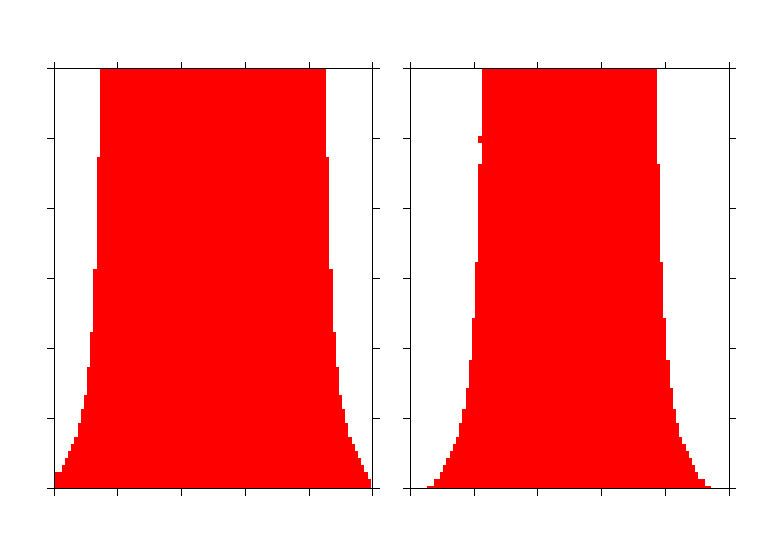
\includegraphics{Figures/Lattice.singlewire/Delta0.0/xifilldepend}}%
    \gplfronttext
  \end{picture}%
\endgroup

\caption{Phase diagrams for $G = 4$ and $G = 8$ as a function of the filling fraction $n = N_F / N$ and the coherence length $\xi$. In white: $\nu = 0$. In red: $\nu = 1$. We notice that the phase diagram for a stronger interaction exhibits a narrower window of the topological nontrivial phase $\nu = 1$. Number of sites: $N = 100$. }
\label{fig.phasediagram.t20}
\end{center}
\end{figure}

First, the symmetry around $n = 1/2$ was discussed in section \ref{sec.fillingfractionsymmetry.breakdown}. Here we showed that letting $n \to 1 - n$ is a symmetry of the system, if we let $\mu \to -\mu$ and $\Delta_{k} \to \Delta_{k + \pi/d}$. The topological invariant is protected under this symmetry for the following two reasons. Firstly, if $\varepsilon_k(\mu) = -t_1\cos(kd) - \mu$ crosses zero, then so does $\varepsilon_k(-\mu)$. Secondly, the pairing is simply shifted by $\pi / d$. This means there is still a contribution of $\text{sgn}(\Delta_{k_1+\pi/d})$ to the invariant from the zero of $\varepsilon_k$ in $k_1$.

Secondly, for a stronger interaction strength, $G$, the window of the topological phase narrows. The reason is that when there is a nonzero interaction, the band $-t_1\cos(kd)$ can be populated even though $\mu$ is below the minimum of the band, i.e. $\mu < -t_1$. For a stronger interaction still, this population starts for lower and lower $\mu$ and there is a larger and larger region of filling fractions $n$, where $\varepsilon_k = -t_1\cos(kd) - \mu$ is strictly positive. This is the topologically trivial region which consequently becomes wider in terms of the corresponding filling fractions. The argument for the coherence length follows the same logic, since a larger coherence length corresponds to a larger range of the interaction which is qualitatively equivalent to a stronger interaction. 

The effects of higher interaction strength and longer coherence length are the same at $n$ and $1 - n$, because of the filling fraction symmetry. They can be confirmed by studying the dependency $\mu(n)$, e.g. for $G = 0, G = 4$ and $G = 8$. This results in figure \ref{fig.mun.t20.Gdepend}. We clearly observe a nonzero population in the regions with $|\mu| > t_1$ for nonzero interactions, and an increase in the size of these regions with increasing interaction strength. Studying the effect of an increase in $\xi$ confirms that the effect hereof is essentially the same as increasing the strength, $G$.  

\begin{figure}
\begin{center}
% GNUPLOT: LaTeX picture with Postscript
\begingroup
  \makeatletter
  \providecommand\color[2][]{%
    \GenericError{(gnuplot) \space\space\space\@spaces}{%
      Package color not loaded in conjunction with
      terminal option `colourtext'%
    }{See the gnuplot documentation for explanation.%
    }{Either use 'blacktext' in gnuplot or load the package
      color.sty in LaTeX.}%
    \renewcommand\color[2][]{}%
  }%
  \providecommand\includegraphics[2][]{%
    \GenericError{(gnuplot) \space\space\space\@spaces}{%
      Package graphicx or graphics not loaded%
    }{See the gnuplot documentation for explanation.%
    }{The gnuplot epslatex terminal needs graphicx.sty or graphics.sty.}%
    \renewcommand\includegraphics[2][]{}%
  }%
  \providecommand\rotatebox[2]{#2}%
  \@ifundefined{ifGPcolor}{%
    \newif\ifGPcolor
    \GPcolorfalse
  }{}%
  \@ifundefined{ifGPblacktext}{%
    \newif\ifGPblacktext
    \GPblacktexttrue
  }{}%
  % define a \g@addto@macro without @ in the name:
  \let\gplgaddtomacro\g@addto@macro
  % define empty templates for all commands taking text:
  \gdef\gplbacktext{}%
  \gdef\gplfronttext{}%
  \makeatother
  \ifGPblacktext
    % no textcolor at all
    \def\colorrgb#1{}%
    \def\colorgray#1{}%
  \else
    % gray or color?
    \ifGPcolor
      \def\colorrgb#1{\color[rgb]{#1}}%
      \def\colorgray#1{\color[gray]{#1}}%
      \expandafter\def\csname LTw\endcsname{\color{white}}%
      \expandafter\def\csname LTb\endcsname{\color{black}}%
      \expandafter\def\csname LTa\endcsname{\color{black}}%
      \expandafter\def\csname LT0\endcsname{\color[rgb]{1,0,0}}%
      \expandafter\def\csname LT1\endcsname{\color[rgb]{0,1,0}}%
      \expandafter\def\csname LT2\endcsname{\color[rgb]{0,0,1}}%
      \expandafter\def\csname LT3\endcsname{\color[rgb]{1,0,1}}%
      \expandafter\def\csname LT4\endcsname{\color[rgb]{0,1,1}}%
      \expandafter\def\csname LT5\endcsname{\color[rgb]{1,1,0}}%
      \expandafter\def\csname LT6\endcsname{\color[rgb]{0,0,0}}%
      \expandafter\def\csname LT7\endcsname{\color[rgb]{1,0.3,0}}%
      \expandafter\def\csname LT8\endcsname{\color[rgb]{0.5,0.5,0.5}}%
    \else
      % gray
      \def\colorrgb#1{\color{black}}%
      \def\colorgray#1{\color[gray]{#1}}%
      \expandafter\def\csname LTw\endcsname{\color{white}}%
      \expandafter\def\csname LTb\endcsname{\color{black}}%
      \expandafter\def\csname LTa\endcsname{\color{black}}%
      \expandafter\def\csname LT0\endcsname{\color{black}}%
      \expandafter\def\csname LT1\endcsname{\color{black}}%
      \expandafter\def\csname LT2\endcsname{\color{black}}%
      \expandafter\def\csname LT3\endcsname{\color{black}}%
      \expandafter\def\csname LT4\endcsname{\color{black}}%
      \expandafter\def\csname LT5\endcsname{\color{black}}%
      \expandafter\def\csname LT6\endcsname{\color{black}}%
      \expandafter\def\csname LT7\endcsname{\color{black}}%
      \expandafter\def\csname LT8\endcsname{\color{black}}%
    \fi
  \fi
    \setlength{\unitlength}{0.0500bp}%
    \ifx\gptboxheight\undefined%
      \newlength{\gptboxheight}%
      \newlength{\gptboxwidth}%
      \newsavebox{\gptboxtext}%
    \fi%
    \setlength{\fboxrule}{0.5pt}%
    \setlength{\fboxsep}{1pt}%
\begin{picture}(7200.00,5040.00)%
    \gplgaddtomacro\gplbacktext{%
      \csname LTb\endcsname%
      \put(682,1188){\makebox(0,0)[r]{\strut{}$-2$}}%
      \csname LTb\endcsname%
      \put(682,2030){\makebox(0,0)[r]{\strut{}$-1$}}%
      \csname LTb\endcsname%
      \put(682,2872){\makebox(0,0)[r]{\strut{}$0$}}%
      \csname LTb\endcsname%
      \put(682,3713){\makebox(0,0)[r]{\strut{}$1$}}%
      \csname LTb\endcsname%
      \put(682,4555){\makebox(0,0)[r]{\strut{}$2$}}%
      \csname LTb\endcsname%
      \put(877,484){\makebox(0,0){\strut{}$0$}}%
      \csname LTb\endcsname%
      \put(2050,484){\makebox(0,0){\strut{}$0.2$}}%
      \csname LTb\endcsname%
      \put(3222,484){\makebox(0,0){\strut{}$0.4$}}%
      \csname LTb\endcsname%
      \put(4395,484){\makebox(0,0){\strut{}$0.6$}}%
      \csname LTb\endcsname%
      \put(5567,484){\makebox(0,0){\strut{}$0.8$}}%
      \csname LTb\endcsname%
      \put(6740,484){\makebox(0,0){\strut{}$1$}}%
    }%
    \gplgaddtomacro\gplfronttext{%
      \csname LTb\endcsname%
      \put(176,2871){\rotatebox{-270}{\makebox(0,0){\strut{}$\mu$}}}%
      \put(3808,154){\makebox(0,0){\strut{}$n$}}%
      \csname LTb\endcsname%
      \put(1933,4803){\makebox(0,0)[r]{\strut{}$G = 0.0$}}%
      \csname LTb\endcsname%
      \put(1933,4583){\makebox(0,0)[r]{\strut{}$G = 2.0$}}%
      \csname LTb\endcsname%
      \put(1933,4363){\makebox(0,0)[r]{\strut{}$G = 4.0$}}%
      \csname LTb\endcsname%
      \put(1933,4143){\makebox(0,0)[r]{\strut{}$G = 8.0$}}%
    }%
    \gplbacktext
    \put(0,0){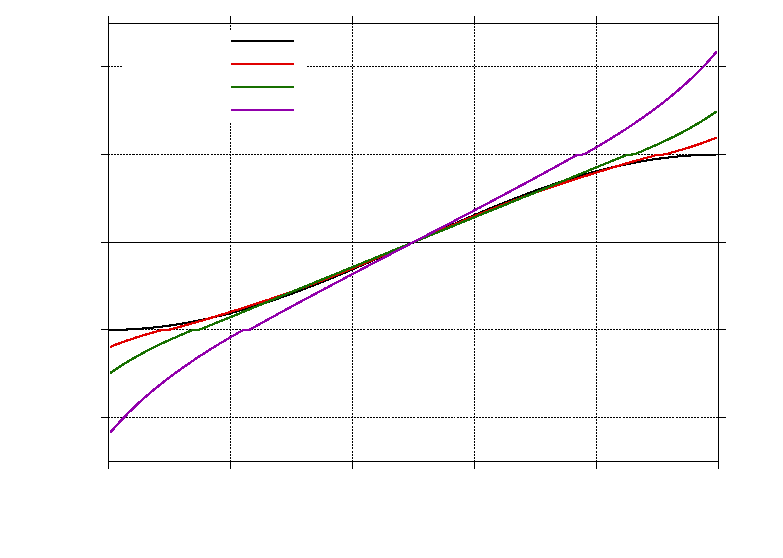
\includegraphics{Figures/Lattice.singlewire/Delta.mu.n0Gvary/ndepend}}%
    \gplfronttext
  \end{picture}%
\endgroup

\caption{The chemical potential, $\mu$, as a function of filling fraction, $n$, for different interaction strengths, $G$. We notice that for nonzero interaction strengths the lattice starts populating for $|\mu| > t_1$. There is a topological phase transition exactly at $|\mu| = t_1$. $\nu = 1$ for $|\mu|< t_1$ and $\nu = 0$ for $|\mu| > t_1$. Other parameters: $N = 100, \xi / d = 5.0$}
\label{fig.mun.t20.Gdepend}
\end{center}
\end{figure}

\section{Next-nearest neighbour hopping included}
\label{sec.NNNincluded} 
In this section the program is very similar to the above. Now however, we include the next-nearest neighbour hopping, i.e. $t_2 \neq 0$. Our main motivation is to look for ground states with winding numbers larger than 1. We produce two sets of phase diagrams, one for $t_2 = t_1$ and one for $t_2 = 0.63t_1$. The latter value seems rather arbitrary, but is chosen since the desired region with winding number $\nu = 2$ is significantly smaller here but still present. For these two values of $t_2$ we do the following. First, we search for the same solution as above, i.e. the start guess is $\Delta_k \propto \sin(kd)$. This produces the phase diagrams to the right in figures \ref{fig.phasediagram.t21.0} and \ref{fig.phasediagram.t20.63}. Next we search for a solutions with $\sin(2kd)$-like behaviour. This results in the phase diagrams to the left. The topological invariant is calculated according to equation \eqref{eq.topologicalinvariant}. We go into more detail with this below. The phase diagrams given in these two figures are one of the main results of the present thesis. The most apparent difference to the case of absent next-nearest neighbour hopping, $t_2 = 0$, treated in the previous section is that the symmetry around $n = 1 / 2$ is broken. This is consistent with the discussion in section \ref{sec.fillingfractionsymmetry.breakdown}.
The most \textit{interesting} part of the figures are the blue regions. These show, where it is possible to find a self-consistent solution with a topological invariant $\nu = 2$. It is exactly this sort of solution we are after! 

\begin{figure}
\begin{center}
% GNUPLOT: LaTeX picture with Postscript
\begingroup
  \makeatletter
  \providecommand\color[2][]{%
    \GenericError{(gnuplot) \space\space\space\@spaces}{%
      Package color not loaded in conjunction with
      terminal option `colourtext'%
    }{See the gnuplot documentation for explanation.%
    }{Either use 'blacktext' in gnuplot or load the package
      color.sty in LaTeX.}%
    \renewcommand\color[2][]{}%
  }%
  \providecommand\includegraphics[2][]{%
    \GenericError{(gnuplot) \space\space\space\@spaces}{%
      Package graphicx or graphics not loaded%
    }{See the gnuplot documentation for explanation.%
    }{The gnuplot epslatex terminal needs graphicx.sty or graphics.sty.}%
    \renewcommand\includegraphics[2][]{}%
  }%
  \providecommand\rotatebox[2]{#2}%
  \@ifundefined{ifGPcolor}{%
    \newif\ifGPcolor
    \GPcolorfalse
  }{}%
  \@ifundefined{ifGPblacktext}{%
    \newif\ifGPblacktext
    \GPblacktexttrue
  }{}%
  % define a \g@addto@macro without @ in the name:
  \let\gplgaddtomacro\g@addto@macro
  % define empty templates for all commands taking text:
  \gdef\gplbacktext{}%
  \gdef\gplfronttext{}%
  \makeatother
  \ifGPblacktext
    % no textcolor at all
    \def\colorrgb#1{}%
    \def\colorgray#1{}%
  \else
    % gray or color?
    \ifGPcolor
      \def\colorrgb#1{\color[rgb]{#1}}%
      \def\colorgray#1{\color[gray]{#1}}%
      \expandafter\def\csname LTw\endcsname{\color{white}}%
      \expandafter\def\csname LTb\endcsname{\color{black}}%
      \expandafter\def\csname LTa\endcsname{\color{black}}%
      \expandafter\def\csname LT0\endcsname{\color[rgb]{1,0,0}}%
      \expandafter\def\csname LT1\endcsname{\color[rgb]{0,1,0}}%
      \expandafter\def\csname LT2\endcsname{\color[rgb]{0,0,1}}%
      \expandafter\def\csname LT3\endcsname{\color[rgb]{1,0,1}}%
      \expandafter\def\csname LT4\endcsname{\color[rgb]{0,1,1}}%
      \expandafter\def\csname LT5\endcsname{\color[rgb]{1,1,0}}%
      \expandafter\def\csname LT6\endcsname{\color[rgb]{0,0,0}}%
      \expandafter\def\csname LT7\endcsname{\color[rgb]{1,0.3,0}}%
      \expandafter\def\csname LT8\endcsname{\color[rgb]{0.5,0.5,0.5}}%
    \else
      % gray
      \def\colorrgb#1{\color{black}}%
      \def\colorgray#1{\color[gray]{#1}}%
      \expandafter\def\csname LTw\endcsname{\color{white}}%
      \expandafter\def\csname LTb\endcsname{\color{black}}%
      \expandafter\def\csname LTa\endcsname{\color{black}}%
      \expandafter\def\csname LT0\endcsname{\color{black}}%
      \expandafter\def\csname LT1\endcsname{\color{black}}%
      \expandafter\def\csname LT2\endcsname{\color{black}}%
      \expandafter\def\csname LT3\endcsname{\color{black}}%
      \expandafter\def\csname LT4\endcsname{\color{black}}%
      \expandafter\def\csname LT5\endcsname{\color{black}}%
      \expandafter\def\csname LT6\endcsname{\color{black}}%
      \expandafter\def\csname LT7\endcsname{\color{black}}%
      \expandafter\def\csname LT8\endcsname{\color{black}}%
    \fi
  \fi
    \setlength{\unitlength}{0.0500bp}%
    \ifx\gptboxheight\undefined%
      \newlength{\gptboxheight}%
      \newlength{\gptboxwidth}%
      \newsavebox{\gptboxtext}%
    \fi%
    \setlength{\fboxrule}{0.5pt}%
    \setlength{\fboxsep}{1pt}%
\begin{picture}(7200.00,5040.00)%
    \gplgaddtomacro\gplbacktext{%
      \csname LTb\endcsname%
      \put(165,756){\makebox(0,0)[r]{\strut{}$1$}}%
      \put(165,1386){\makebox(0,0)[r]{\strut{}$2$}}%
      \put(165,2016){\makebox(0,0)[r]{\strut{}$3$}}%
      \put(165,2646){\makebox(0,0)[r]{\strut{}$4$}}%
      \put(165,3275){\makebox(0,0)[r]{\strut{}$5$}}%
      \put(165,3905){\makebox(0,0)[r]{\strut{}$6$}}%
      \put(165,4535){\makebox(0,0)[r]{\strut{}$7$}}%
      \put(360,473){\makebox(0,0){\strut{}$0$}}%
      \put(972,473){\makebox(0,0){\strut{}$0.2$}}%
      \put(1584,473){\makebox(0,0){\strut{}$0.4$}}%
      \put(2195,473){\makebox(0,0){\strut{}$0.6$}}%
      \put(2807,473){\makebox(0,0){\strut{}$0.8$}}%
      \put(3419,473){\makebox(0,0){\strut{}$1$}}%
    }%
    \gplgaddtomacro\gplfronttext{%
      \csname LTb\endcsname%
      \put(-209,2645){\rotatebox{-270}{\makebox(0,0){\strut{}$\xi / d$}}}%
      \put(1889,143){\makebox(0,0){\strut{}$n$}}%
      \put(1889,4928){\makebox(0,0){\strut{}$t_2 = t_1, \text{anomalous}$}}%
      \put(972,3590){\makebox(0,0){\color{white}\strut{}$\nu = 1$}}%
      \put(1889, 3590){\makebox(0,0){\color{white}\strut{}$\nu = 2$}}%
      \put(2807,3590){\makebox(0,0){\strut{}$\nu = 0$}}%
      \put(972,3275){\makebox(0,0){\color{white}\strut{}$\times$}}%
      \put(1890,3275){\makebox(0,0){\color{white}\strut{}$*$}}%
    }%
    \gplgaddtomacro\gplbacktext{%
      \csname LTb\endcsname%
      \put(3584,756){\makebox(0,0)[r]{\strut{} }}%
      \put(3584,1386){\makebox(0,0)[r]{\strut{} }}%
      \put(3584,2016){\makebox(0,0)[r]{\strut{} }}%
      \put(3584,2646){\makebox(0,0)[r]{\strut{} }}%
      \put(3584,3275){\makebox(0,0)[r]{\strut{} }}%
      \put(3584,3905){\makebox(0,0)[r]{\strut{} }}%
      \put(3584,4535){\makebox(0,0)[r]{\strut{} }}%
      \put(3779,473){\makebox(0,0){\strut{}$0$}}%
      \put(4391,473){\makebox(0,0){\strut{}$0.2$}}%
      \put(5003,473){\makebox(0,0){\strut{}$0.4$}}%
      \put(5615,473){\makebox(0,0){\strut{}$0.6$}}%
      \put(6227,473){\makebox(0,0){\strut{}$0.8$}}%
      \put(6839,473){\makebox(0,0){\strut{}$1$}}%
    }%
    \gplgaddtomacro\gplfronttext{%
      \csname LTb\endcsname%
      \put(5309,143){\makebox(0,0){\strut{}$n$}}%
      \put(5309,4928){\makebox(0,0){\strut{}$t_2 = t_1, \text{normal}$}}%
      \put(4391,3590){\makebox(0,0){\color{white}\strut{}$\nu = 1$}}%
      \put(6227,3590){\makebox(0,0){\strut{}$\nu = 0$}}%
      \put(4391,3275){\makebox(0,0){\color{white}\strut{}$\times$}}%
      \put(5309,3275){\makebox(0,0){\strut{}$*$}}%
    }%
    \gplbacktext
    \put(0,0){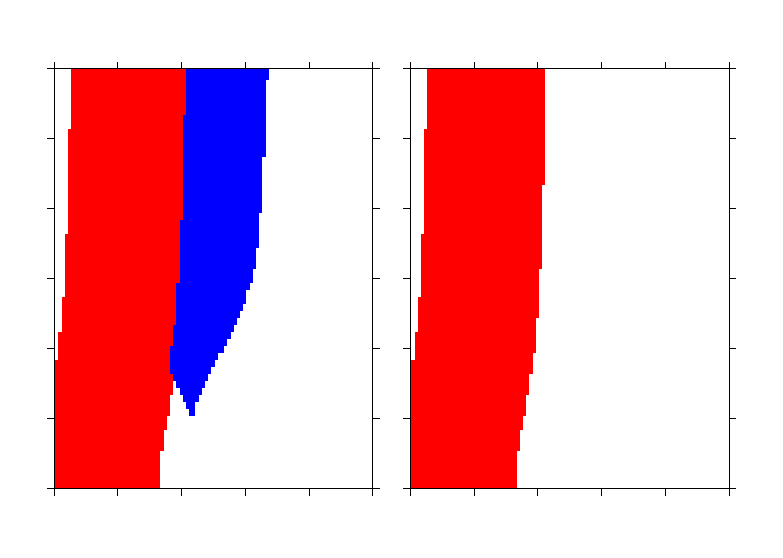
\includegraphics{Figures/Lattice.singlewire/t2nonzerophasediagrams/xifilldepend1}}%
    \gplfronttext
  \end{picture}%
\endgroup

\caption{Topological phase diagram for $t_2 = t_1$ as a function of the filling fraction $n = N_F/N$ and coherence length $\xi$. Invariant: in white: $\nu = 0$, in red: $\nu = 1$, in blue: $\nu = 2$. The pairing is shown for the points $\times$ and $*$ in figure \ref{fig.Deltaexamples.t21.0}. To the left: (anomalous) result of searching for $\Delta_k \propto \sin(2kd)$-like solutions. To the right: (normal) result of searching for $\Delta_k \propto \sin(kd)$-like solutions. The algorithm is a little uncertain around the blue tip at $n \approx 0.4, \xi / d \approx 2$. The phase has here been checked by doubling the number of lattice sites. Other parameters: $G = 4$, $N = 100$. }
\label{fig.phasediagram.t21.0}
\vspace{0.5cm}
% GNUPLOT: LaTeX picture with Postscript
\begingroup
  \makeatletter
  \providecommand\color[2][]{%
    \GenericError{(gnuplot) \space\space\space\@spaces}{%
      Package color not loaded in conjunction with
      terminal option `colourtext'%
    }{See the gnuplot documentation for explanation.%
    }{Either use 'blacktext' in gnuplot or load the package
      color.sty in LaTeX.}%
    \renewcommand\color[2][]{}%
  }%
  \providecommand\includegraphics[2][]{%
    \GenericError{(gnuplot) \space\space\space\@spaces}{%
      Package graphicx or graphics not loaded%
    }{See the gnuplot documentation for explanation.%
    }{The gnuplot epslatex terminal needs graphicx.sty or graphics.sty.}%
    \renewcommand\includegraphics[2][]{}%
  }%
  \providecommand\rotatebox[2]{#2}%
  \@ifundefined{ifGPcolor}{%
    \newif\ifGPcolor
    \GPcolorfalse
  }{}%
  \@ifundefined{ifGPblacktext}{%
    \newif\ifGPblacktext
    \GPblacktexttrue
  }{}%
  % define a \g@addto@macro without @ in the name:
  \let\gplgaddtomacro\g@addto@macro
  % define empty templates for all commands taking text:
  \gdef\gplbacktext{}%
  \gdef\gplfronttext{}%
  \makeatother
  \ifGPblacktext
    % no textcolor at all
    \def\colorrgb#1{}%
    \def\colorgray#1{}%
  \else
    % gray or color?
    \ifGPcolor
      \def\colorrgb#1{\color[rgb]{#1}}%
      \def\colorgray#1{\color[gray]{#1}}%
      \expandafter\def\csname LTw\endcsname{\color{white}}%
      \expandafter\def\csname LTb\endcsname{\color{black}}%
      \expandafter\def\csname LTa\endcsname{\color{black}}%
      \expandafter\def\csname LT0\endcsname{\color[rgb]{1,0,0}}%
      \expandafter\def\csname LT1\endcsname{\color[rgb]{0,1,0}}%
      \expandafter\def\csname LT2\endcsname{\color[rgb]{0,0,1}}%
      \expandafter\def\csname LT3\endcsname{\color[rgb]{1,0,1}}%
      \expandafter\def\csname LT4\endcsname{\color[rgb]{0,1,1}}%
      \expandafter\def\csname LT5\endcsname{\color[rgb]{1,1,0}}%
      \expandafter\def\csname LT6\endcsname{\color[rgb]{0,0,0}}%
      \expandafter\def\csname LT7\endcsname{\color[rgb]{1,0.3,0}}%
      \expandafter\def\csname LT8\endcsname{\color[rgb]{0.5,0.5,0.5}}%
    \else
      % gray
      \def\colorrgb#1{\color{black}}%
      \def\colorgray#1{\color[gray]{#1}}%
      \expandafter\def\csname LTw\endcsname{\color{white}}%
      \expandafter\def\csname LTb\endcsname{\color{black}}%
      \expandafter\def\csname LTa\endcsname{\color{black}}%
      \expandafter\def\csname LT0\endcsname{\color{black}}%
      \expandafter\def\csname LT1\endcsname{\color{black}}%
      \expandafter\def\csname LT2\endcsname{\color{black}}%
      \expandafter\def\csname LT3\endcsname{\color{black}}%
      \expandafter\def\csname LT4\endcsname{\color{black}}%
      \expandafter\def\csname LT5\endcsname{\color{black}}%
      \expandafter\def\csname LT6\endcsname{\color{black}}%
      \expandafter\def\csname LT7\endcsname{\color{black}}%
      \expandafter\def\csname LT8\endcsname{\color{black}}%
    \fi
  \fi
    \setlength{\unitlength}{0.0500bp}%
    \ifx\gptboxheight\undefined%
      \newlength{\gptboxheight}%
      \newlength{\gptboxwidth}%
      \newsavebox{\gptboxtext}%
    \fi%
    \setlength{\fboxrule}{0.5pt}%
    \setlength{\fboxsep}{1pt}%
\begin{picture}(7200.00,5040.00)%
    \gplgaddtomacro\gplbacktext{%
      \csname LTb\endcsname%
      \put(165,756){\makebox(0,0)[r]{\strut{}$1$}}%
      \put(165,1386){\makebox(0,0)[r]{\strut{}$2$}}%
      \put(165,2016){\makebox(0,0)[r]{\strut{}$3$}}%
      \put(165,2646){\makebox(0,0)[r]{\strut{}$4$}}%
      \put(165,3275){\makebox(0,0)[r]{\strut{}$5$}}%
      \put(165,3905){\makebox(0,0)[r]{\strut{}$6$}}%
      \put(165,4535){\makebox(0,0)[r]{\strut{}$7$}}%
      \put(360,473){\makebox(0,0){\strut{}$0$}}%
      \put(972,473){\makebox(0,0){\strut{}$0.2$}}%
      \put(1584,473){\makebox(0,0){\strut{}$0.4$}}%
      \put(2195,473){\makebox(0,0){\strut{}$0.6$}}%
      \put(2807,473){\makebox(0,0){\strut{}$0.8$}}%
      \put(3419,473){\makebox(0,0){\strut{}$1$}}%
    }%
    \gplgaddtomacro\gplfronttext{%
      \csname LTb\endcsname%
      \put(-209,2645){\rotatebox{-270}{\makebox(0,0){\strut{}$\xi / d$}}}%
      \put(1889,143){\makebox(0,0){\strut{}$n$}}%
      \put(1889,4928){\makebox(0,0){\strut{}$t_2 = 0.63t_1, \text{anomalous}$}}%
    }%
    \gplgaddtomacro\gplbacktext{%
      \csname LTb\endcsname%
      \put(3584,756){\makebox(0,0)[r]{\strut{} }}%
      \put(3584,1386){\makebox(0,0)[r]{\strut{} }}%
      \put(3584,2016){\makebox(0,0)[r]{\strut{} }}%
      \put(3584,2646){\makebox(0,0)[r]{\strut{} }}%
      \put(3584,3275){\makebox(0,0)[r]{\strut{} }}%
      \put(3584,3905){\makebox(0,0)[r]{\strut{} }}%
      \put(3584,4535){\makebox(0,0)[r]{\strut{} }}%
      \put(3779,473){\makebox(0,0){\strut{}$0$}}%
      \put(4391,473){\makebox(0,0){\strut{}$0.2$}}%
      \put(5003,473){\makebox(0,0){\strut{}$0.4$}}%
      \put(5615,473){\makebox(0,0){\strut{}$0.6$}}%
      \put(6227,473){\makebox(0,0){\strut{}$0.8$}}%
      \put(6839,473){\makebox(0,0){\strut{}$1$}}%
    }%
    \gplgaddtomacro\gplfronttext{%
      \csname LTb\endcsname%
      \put(5309,143){\makebox(0,0){\strut{}$n$}}%
      \put(5309,4928){\makebox(0,0){\strut{}$t_2 = 0.63t_1, \text{normal}$}}%
    }%
    \gplbacktext
    \put(0,0){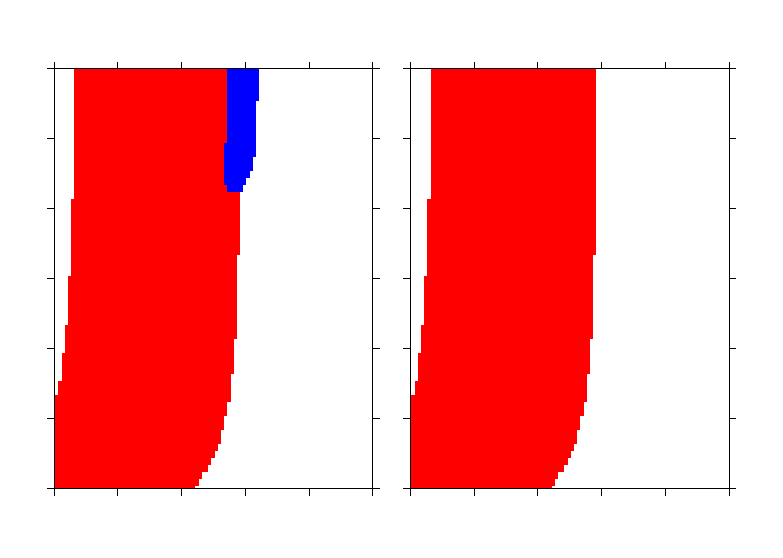
\includegraphics{Figures/Lattice.singlewire/t2nonzerophasediagrams/xifilldepend2}}%
    \gplfronttext
  \end{picture}%
\endgroup

\caption{Topological phase diagrams for $t_2 = 0.63t_1$ as a function of the filling fraction $n = N_F/N$ and coherence length $\xi$. In white: $\nu = 0$, in red: $\nu = 1$, in blue: $\nu = 2$. To the left: (anomalous) result of searching for $\Delta_k\propto \sin(2kd)$-like solutions. To the right: (normal) result of searching for $\Delta_k \propto \sin(kd)$-like solutions. Other parameters: $G = 4$, $N = 100$. }
\label{fig.phasediagram.t20.63}
\end{center}
\end{figure}

In figure \ref{fig.Deltaexamples.t21.0} we go into more detail with the pairing at the points $\times$ and $*$ specified in the phase diagrams in figure \ref{fig.phasediagram.t21.0}. Point $\times$ is in the $\nu = 1$ phase, whilst point $*$ can either be in the $\nu = 0$ or the $\nu = 2$ phase. Remember that the topological invariant depends on how both the kinetic energy, $\varepsilon_k$, and the pairing, $\Delta_k$, behave in the first Brillouin zone. Every zero of $\varepsilon_k$ for $k > 0$ contributes the sign of the pairing times the sign of the slope of $\varepsilon_k$:
\begin{equation}
\nu = \left| \text{sgn}\left(\Delta_{k_1}\partial_k\varepsilon_{k = k_1}\right) + \text{sgn}\left(\Delta_{k_1}\partial_k\varepsilon_{k = k_2}\right)\right|, 
\label{eq.windingnumber.lattice.twozeros}
\end{equation}
where $k_1 > 0$ and $k_2 > 0$ are the positive $k$-values where $\varepsilon_k = 0$.\footnote{We could also use the negative $k$-values $-k_1, -k_2$.} Now at $\times$ we only find one solution for the pairing, irrespective of the initial guess. This can be seen from figure \ref{fig.Deltaexamples.t21.0}(left). This single solution is $\sin(kd)$-like in that it only crosses zero at $k = 0$. There is only one positive zero of $\varepsilon_k$, so the invariant is $\nu = 1$. This behaviour is not general for the entire red region of topological invariant $\nu = 1$. Closer to the point $*$, but still in the red region, we indeed find $\sin(2kd)$-like solutions. These however still have $\nu = 1$, because the filling fraction is too low to make an additional pair of zeroes of $\varepsilon_k$. At $*$ we find two solutions for the pairing, as is evident from figure \ref{fig.Deltaexamples.t21.0}(right). Here both a (normal) $\sin(kd)$- and an (anomalous) $\sin(2kd)$-like solution are self-consistent. Since $\varepsilon_k$ now has two pairs of zeroes, the topological invariant is $\nu = 0$ and $\nu = 2$ for the normal and anomalous pairing respectively. This is because the pairing must change sign in-between the zeroes of $\varepsilon_k$ to produce a $\nu = 2$ phase as evident from equation \eqref{eq.windingnumber.lattice.twozeros} and the discussion in the end of chapter \ref{Chapter7}. 

\begin{figure}
\begin{center}
% GNUPLOT: LaTeX picture with Postscript
\begingroup
  \makeatletter
  \providecommand\color[2][]{%
    \GenericError{(gnuplot) \space\space\space\@spaces}{%
      Package color not loaded in conjunction with
      terminal option `colourtext'%
    }{See the gnuplot documentation for explanation.%
    }{Either use 'blacktext' in gnuplot or load the package
      color.sty in LaTeX.}%
    \renewcommand\color[2][]{}%
  }%
  \providecommand\includegraphics[2][]{%
    \GenericError{(gnuplot) \space\space\space\@spaces}{%
      Package graphicx or graphics not loaded%
    }{See the gnuplot documentation for explanation.%
    }{The gnuplot epslatex terminal needs graphicx.sty or graphics.sty.}%
    \renewcommand\includegraphics[2][]{}%
  }%
  \providecommand\rotatebox[2]{#2}%
  \@ifundefined{ifGPcolor}{%
    \newif\ifGPcolor
    \GPcolorfalse
  }{}%
  \@ifundefined{ifGPblacktext}{%
    \newif\ifGPblacktext
    \GPblacktexttrue
  }{}%
  % define a \g@addto@macro without @ in the name:
  \let\gplgaddtomacro\g@addto@macro
  % define empty templates for all commands taking text:
  \gdef\gplbacktext{}%
  \gdef\gplfronttext{}%
  \makeatother
  \ifGPblacktext
    % no textcolor at all
    \def\colorrgb#1{}%
    \def\colorgray#1{}%
  \else
    % gray or color?
    \ifGPcolor
      \def\colorrgb#1{\color[rgb]{#1}}%
      \def\colorgray#1{\color[gray]{#1}}%
      \expandafter\def\csname LTw\endcsname{\color{white}}%
      \expandafter\def\csname LTb\endcsname{\color{black}}%
      \expandafter\def\csname LTa\endcsname{\color{black}}%
      \expandafter\def\csname LT0\endcsname{\color[rgb]{1,0,0}}%
      \expandafter\def\csname LT1\endcsname{\color[rgb]{0,1,0}}%
      \expandafter\def\csname LT2\endcsname{\color[rgb]{0,0,1}}%
      \expandafter\def\csname LT3\endcsname{\color[rgb]{1,0,1}}%
      \expandafter\def\csname LT4\endcsname{\color[rgb]{0,1,1}}%
      \expandafter\def\csname LT5\endcsname{\color[rgb]{1,1,0}}%
      \expandafter\def\csname LT6\endcsname{\color[rgb]{0,0,0}}%
      \expandafter\def\csname LT7\endcsname{\color[rgb]{1,0.3,0}}%
      \expandafter\def\csname LT8\endcsname{\color[rgb]{0.5,0.5,0.5}}%
    \else
      % gray
      \def\colorrgb#1{\color{black}}%
      \def\colorgray#1{\color[gray]{#1}}%
      \expandafter\def\csname LTw\endcsname{\color{white}}%
      \expandafter\def\csname LTb\endcsname{\color{black}}%
      \expandafter\def\csname LTa\endcsname{\color{black}}%
      \expandafter\def\csname LT0\endcsname{\color{black}}%
      \expandafter\def\csname LT1\endcsname{\color{black}}%
      \expandafter\def\csname LT2\endcsname{\color{black}}%
      \expandafter\def\csname LT3\endcsname{\color{black}}%
      \expandafter\def\csname LT4\endcsname{\color{black}}%
      \expandafter\def\csname LT5\endcsname{\color{black}}%
      \expandafter\def\csname LT6\endcsname{\color{black}}%
      \expandafter\def\csname LT7\endcsname{\color{black}}%
      \expandafter\def\csname LT8\endcsname{\color{black}}%
    \fi
  \fi
    \setlength{\unitlength}{0.0500bp}%
    \ifx\gptboxheight\undefined%
      \newlength{\gptboxheight}%
      \newlength{\gptboxwidth}%
      \newsavebox{\gptboxtext}%
    \fi%
    \setlength{\fboxrule}{0.5pt}%
    \setlength{\fboxsep}{1pt}%
\begin{picture}(7200.00,5040.00)%
    \gplgaddtomacro\gplbacktext{%
      \csname LTb\endcsname%
      \put(165,869){\makebox(0,0)[r]{\strut{}$-2$}}%
      \csname LTb\endcsname%
      \put(165,1600){\makebox(0,0)[r]{\strut{}$-1$}}%
      \csname LTb\endcsname%
      \put(165,2331){\makebox(0,0)[r]{\strut{}$0$}}%
      \csname LTb\endcsname%
      \put(165,3061){\makebox(0,0)[r]{\strut{}$1$}}%
      \csname LTb\endcsname%
      \put(165,3792){\makebox(0,0)[r]{\strut{}$2$}}%
      \csname LTb\endcsname%
      \put(429,221){\makebox(0,0){\strut{}$-3$}}%
      \csname LTb\endcsname%
      \put(916,221){\makebox(0,0){\strut{}$-2$}}%
      \csname LTb\endcsname%
      \put(1403,221){\makebox(0,0){\strut{}$-1$}}%
      \csname LTb\endcsname%
      \put(1890,221){\makebox(0,0){\strut{}$0$}}%
      \csname LTb\endcsname%
      \put(2376,221){\makebox(0,0){\strut{}$1$}}%
      \csname LTb\endcsname%
      \put(2863,221){\makebox(0,0){\strut{}$2$}}%
      \csname LTb\endcsname%
      \put(3350,221){\makebox(0,0){\strut{}$3$}}%
    }%
    \gplgaddtomacro\gplfronttext{%
      \csname LTb\endcsname%
      \put(-341,2330){\rotatebox{-270}{\makebox(0,0){\strut{}$2\Delta_k, \varepsilon_k$}}}%
      \put(1889,-109){\makebox(0,0){\strut{}$kd$}}%
      \put(429,4550){\makebox(0,0){\strut{}$(i)$}}%
      \csname LTb\endcsname%
      \put(670,4867){\makebox(0,0)[l]{\strut{}$\Delta_k/t_1 \sim \sin(1kd)$}}%
      \csname LTb\endcsname%
      \put(670,4647){\makebox(0,0)[l]{\strut{}$\varepsilon_k / t_1$}}%
    }%
    \gplgaddtomacro\gplbacktext{%
      \csname LTb\endcsname%
      \put(3584,869){\makebox(0,0)[r]{\strut{} }}%
      \csname LTb\endcsname%
      \put(3584,1600){\makebox(0,0)[r]{\strut{} }}%
      \csname LTb\endcsname%
      \put(3584,2331){\makebox(0,0)[r]{\strut{} }}%
      \csname LTb\endcsname%
      \put(3584,3061){\makebox(0,0)[r]{\strut{} }}%
      \csname LTb\endcsname%
      \put(3584,3792){\makebox(0,0)[r]{\strut{} }}%
      \csname LTb\endcsname%
      \put(3848,221){\makebox(0,0){\strut{}$-3$}}%
      \csname LTb\endcsname%
      \put(4335,221){\makebox(0,0){\strut{}$-2$}}%
      \csname LTb\endcsname%
      \put(4822,221){\makebox(0,0){\strut{}$-1$}}%
      \csname LTb\endcsname%
      \put(5309,221){\makebox(0,0){\strut{}$0$}}%
      \csname LTb\endcsname%
      \put(5796,221){\makebox(0,0){\strut{}$1$}}%
      \csname LTb\endcsname%
      \put(6283,221){\makebox(0,0){\strut{}$2$}}%
      \csname LTb\endcsname%
      \put(6770,221){\makebox(0,0){\strut{}$3$}}%
    }%
    \gplgaddtomacro\gplfronttext{%
      \csname LTb\endcsname%
      \put(5309,-109){\makebox(0,0){\strut{}$kd$}}%
      \put(3848,4550){\makebox(0,0){\strut{}$(ii)$}}%
      \csname LTb\endcsname%
      \put(4089,4867){\makebox(0,0)[l]{\strut{}$\Delta_k/t_1 \sim \sin(1kd)$}}%
      \csname LTb\endcsname%
      \put(4089,4647){\makebox(0,0)[l]{\strut{}$\Delta_k/t_1 \sim \sin(2kd)$}}%
      \csname LTb\endcsname%
      \put(4089,4427){\makebox(0,0)[l]{\strut{}$\varepsilon_k / t_1$}}%
    }%
    \gplbacktext
    \put(0,0){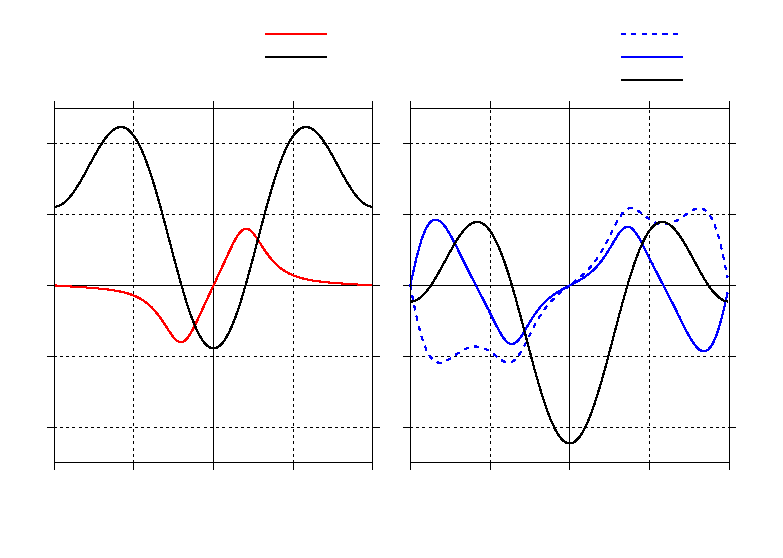
\includegraphics{Figures/Lattice.singlewire/Deltaexamples/kdepend}}%
    \gplfronttext
  \end{picture}%
\endgroup

\caption{The pairing, $\Delta_k$, and kinetic energy, $\varepsilon_k$, across the Brillouin zone. In black: $\varepsilon_k$. Left: point $\times$ in figure \ref{fig.phasediagram.t21.0}. Red solid line: only one solution for $\Delta_k$. This is $\sin(kd)$-like. Topological invariant: $\nu = 1$. Right: point $*$ in figure \ref{fig.phasediagram.t21.0}. Blue lines: two solutions for $\Delta_k$. Dashed blue line: $\sin(kd)$-like solution with $\nu = 0$. Solid blue line: $\sin(2kd)$-like solution with $\nu = 2$. Notice that the pairing is maximal around the zeroes of $\varepsilon_k$. Parameters: $t_2 = t_1$, $G = 4$, $N = 100$, $\xi / d = 5$. $\times$: $n = 0.2$, $*$: $n = 0.5$.}
\label{fig.Deltaexamples.t21.0}
\end{center}
\end{figure}

The occurrence of the anomalous $\nu = 2$ phase is at high filling and long coherence lengths. The former condition we already discussed above. We must have a high filling fraction to produce two pairs of zero points of $\varepsilon_k$. The latter condition we can understand by transforming the pairing to real space. The relevant term in the Hamiltonian has the form $\sum_k \Delta_k c_{-k}c_{k}$. Plugging in $c_k = \frac{1}{\sqrt{N}}\sum_j \text{e}^{-ikx_j}x_j$, with $x_j = jd$ we get:
\begin{equation}
\sum_k \Delta_k c_{-k}c_{k} = \sum_{j,l} \tilde{\Delta}_{j,l}c_jc_l, \hspace{0.5cm} \tilde{\Delta}_{j,l} = \frac{1}{N}\sum_k\Delta_k\text{e}^{ik(x_j-x_l)}. \nonumber
\end{equation}
Hence, the real space pairing is quite simply the Fourier transform of the momentum space pairing. We use the orthogonality of $\sin(lkd)$ for different $l$ to get the following. For $\Delta_k = \Delta_1\sin(kd)$ we get $\tilde{\Delta}_{0,1} = -\tilde{\Delta}_{1,0} = -i\frac{\Delta_1}{2}$ with all others zero. In the same manner for $\Delta_k = \Delta_2\sin(2kd)$ we get $\tilde{\Delta}_{0,2} = -\tilde{\Delta}_{2,0} = -i\frac{\Delta_2}{2}$ with all others zero. Spelled out this means that a $\sin(kd)$-like pairing has dominant \textit{nearest} neighbour pairing, whereas a $\sin(2kd)$-like pairing has dominant \text{next-nearest} neighbour pairing. This explains, why we must go to long coherence lengths. We simply need a long-range interaction for the particles to dominantly be able to pair with next-nearest neighbours. In turn a $\sin(2kd)$-like pairing in momentum space forms and the $\nu = 2$ phase is realized if the filling fraction is large as well, as discussed above. 

Now we can also explain, why the $\nu = 2$ phase region is larger for larger $t_2$ as can be seen by comparing figure \ref{fig.phasediagram.t21.0}(left) and figure \ref{fig.phasediagram.t20.63}(left). The above analysis shows that we need a window of two zeroes of the kinetic energy, $\varepsilon_k$. This window is simply larger for increasing $t_2$, since the kinetic energy decreaes more at the Brillouin zone boundary. As $t_2$ \textit{de}creases, this window narrows, and moves to higher filling fractions and coherence lengths. 

Since we found two different self-consistent solutions, $\Delta_k \sim \sin(kd)$ and $\Delta_k \sim \sin(2kd)$, for certain parameters we need to figure out which one has the lowest energy. The ground state energy, $E_0$, is given by: 

\begin{equation}
E_0 - \mu N_F = \frac{1}{2}\sum_k \left[\varepsilon_k - E_{F,k} - \Delta_k\braket{c^\dagger_{k}c^\dagger_{-k}}\right] = -\frac{1}{4}\sum_k \frac{1}{E_{F,k}}\left( \varepsilon_k - E_{F,k} \right)^2, \hspace{0.5cm} T = 0, 
\label{eq.groundstategrandenergy.sumformula}
\end{equation}
where we use that $\braket{c_kc_{-k}} = \frac{\Delta_k}{2E_{F,k}}$ at zero temperature. It would be highly interesting, if the $\nu = 2$ phase could be energetically favourable in some parameter region. We therefore plot the relative difference $(E_{0,2} - E_{0,1})/|E_{0,1}|$, where $E_{0,l}$ is the energy when we search for a solution of the form $\Delta_k \sim \sin(lkd)$. Hence, $E_{0,1}$ and $E_{0,2}$ correspond to the diagrams on the right and left in figure \ref{fig.phasediagram.t21.0} respectively. The result of this analysis for $t_2 = t_1$ is given in figure \ref{fig.energydifference.t21.0}. This explicitly shows that the $\nu = 2$ phase is unfortunately \textit{not} energetically favourable. Further, we notice that the higher the filling, the larger the relative difference. However, the figure also shows this difference to be within $6\%$. This makes it plausible that one can make the $\nu = 2$ phase favourable through some perturbation of the system.   

\begin{figure}
\begin{center}
% GNUPLOT: LaTeX picture with Postscript
\begingroup
  \makeatletter
  \providecommand\color[2][]{%
    \GenericError{(gnuplot) \space\space\space\@spaces}{%
      Package color not loaded in conjunction with
      terminal option `colourtext'%
    }{See the gnuplot documentation for explanation.%
    }{Either use 'blacktext' in gnuplot or load the package
      color.sty in LaTeX.}%
    \renewcommand\color[2][]{}%
  }%
  \providecommand\includegraphics[2][]{%
    \GenericError{(gnuplot) \space\space\space\@spaces}{%
      Package graphicx or graphics not loaded%
    }{See the gnuplot documentation for explanation.%
    }{The gnuplot epslatex terminal needs graphicx.sty or graphics.sty.}%
    \renewcommand\includegraphics[2][]{}%
  }%
  \providecommand\rotatebox[2]{#2}%
  \@ifundefined{ifGPcolor}{%
    \newif\ifGPcolor
    \GPcolorfalse
  }{}%
  \@ifundefined{ifGPblacktext}{%
    \newif\ifGPblacktext
    \GPblacktexttrue
  }{}%
  % define a \g@addto@macro without @ in the name:
  \let\gplgaddtomacro\g@addto@macro
  % define empty templates for all commands taking text:
  \gdef\gplbacktext{}%
  \gdef\gplfronttext{}%
  \makeatother
  \ifGPblacktext
    % no textcolor at all
    \def\colorrgb#1{}%
    \def\colorgray#1{}%
  \else
    % gray or color?
    \ifGPcolor
      \def\colorrgb#1{\color[rgb]{#1}}%
      \def\colorgray#1{\color[gray]{#1}}%
      \expandafter\def\csname LTw\endcsname{\color{white}}%
      \expandafter\def\csname LTb\endcsname{\color{black}}%
      \expandafter\def\csname LTa\endcsname{\color{black}}%
      \expandafter\def\csname LT0\endcsname{\color[rgb]{1,0,0}}%
      \expandafter\def\csname LT1\endcsname{\color[rgb]{0,1,0}}%
      \expandafter\def\csname LT2\endcsname{\color[rgb]{0,0,1}}%
      \expandafter\def\csname LT3\endcsname{\color[rgb]{1,0,1}}%
      \expandafter\def\csname LT4\endcsname{\color[rgb]{0,1,1}}%
      \expandafter\def\csname LT5\endcsname{\color[rgb]{1,1,0}}%
      \expandafter\def\csname LT6\endcsname{\color[rgb]{0,0,0}}%
      \expandafter\def\csname LT7\endcsname{\color[rgb]{1,0.3,0}}%
      \expandafter\def\csname LT8\endcsname{\color[rgb]{0.5,0.5,0.5}}%
    \else
      % gray
      \def\colorrgb#1{\color{black}}%
      \def\colorgray#1{\color[gray]{#1}}%
      \expandafter\def\csname LTw\endcsname{\color{white}}%
      \expandafter\def\csname LTb\endcsname{\color{black}}%
      \expandafter\def\csname LTa\endcsname{\color{black}}%
      \expandafter\def\csname LT0\endcsname{\color{black}}%
      \expandafter\def\csname LT1\endcsname{\color{black}}%
      \expandafter\def\csname LT2\endcsname{\color{black}}%
      \expandafter\def\csname LT3\endcsname{\color{black}}%
      \expandafter\def\csname LT4\endcsname{\color{black}}%
      \expandafter\def\csname LT5\endcsname{\color{black}}%
      \expandafter\def\csname LT6\endcsname{\color{black}}%
      \expandafter\def\csname LT7\endcsname{\color{black}}%
      \expandafter\def\csname LT8\endcsname{\color{black}}%
    \fi
  \fi
    \setlength{\unitlength}{0.0500bp}%
    \ifx\gptboxheight\undefined%
      \newlength{\gptboxheight}%
      \newlength{\gptboxwidth}%
      \newsavebox{\gptboxtext}%
    \fi%
    \setlength{\fboxrule}{0.5pt}%
    \setlength{\fboxsep}{1pt}%
\begin{picture}(7200.00,5040.00)%
    \gplgaddtomacro\gplbacktext{%
      \csname LTb\endcsname%
      \put(550,767){\makebox(0,0)[r]{\strut{}$1$}}%
      \csname LTb\endcsname%
      \put(550,1469){\makebox(0,0)[r]{\strut{}$2$}}%
      \csname LTb\endcsname%
      \put(550,2170){\makebox(0,0)[r]{\strut{}$3$}}%
      \csname LTb\endcsname%
      \put(550,2872){\makebox(0,0)[r]{\strut{}$4$}}%
      \csname LTb\endcsname%
      \put(550,3573){\makebox(0,0)[r]{\strut{}$5$}}%
      \csname LTb\endcsname%
      \put(550,4275){\makebox(0,0)[r]{\strut{}$6$}}%
      \csname LTb\endcsname%
      \put(550,4976){\makebox(0,0)[r]{\strut{}$7$}}%
      \csname LTb\endcsname%
      \put(745,484){\makebox(0,0){\strut{}$0$}}%
      \csname LTb\endcsname%
      \put(1741,484){\makebox(0,0){\strut{}$0.2$}}%
      \csname LTb\endcsname%
      \put(2737,484){\makebox(0,0){\strut{}$0.4$}}%
      \csname LTb\endcsname%
      \put(3733,484){\makebox(0,0){\strut{}$0.6$}}%
      \csname LTb\endcsname%
      \put(4729,484){\makebox(0,0){\strut{}$0.8$}}%
      \csname LTb\endcsname%
      \put(5725,484){\makebox(0,0){\strut{}$1$}}%
    }%
    \gplgaddtomacro\gplfronttext{%
      \csname LTb\endcsname%
      \put(176,2871){\rotatebox{-270}{\makebox(0,0){\strut{}$xi / d$}}}%
      \put(3235,154){\makebox(0,0){\strut{}$n$}}%
      \csname LTb\endcsname%
      \put(6483,767){\makebox(0,0)[l]{\strut{}$-0.015$}}%
      \put(6483,1293){\makebox(0,0)[l]{\strut{}$-0.01$}}%
      \put(6483,1819){\makebox(0,0)[l]{\strut{}$-0.005$}}%
      \put(6483,2345){\makebox(0,0)[l]{\strut{}$0$}}%
      \put(6483,2871){\makebox(0,0)[l]{\strut{}$0.005$}}%
      \put(6483,3397){\makebox(0,0)[l]{\strut{}$0.01$}}%
      \put(6483,3923){\makebox(0,0)[l]{\strut{}$0.015$}}%
      \put(6483,4449){\makebox(0,0)[l]{\strut{}$0.02$}}%
      \put(6483,4976){\makebox(0,0)[l]{\strut{}$0.025$}}%
    }%
    \gplbacktext
    \put(0,0){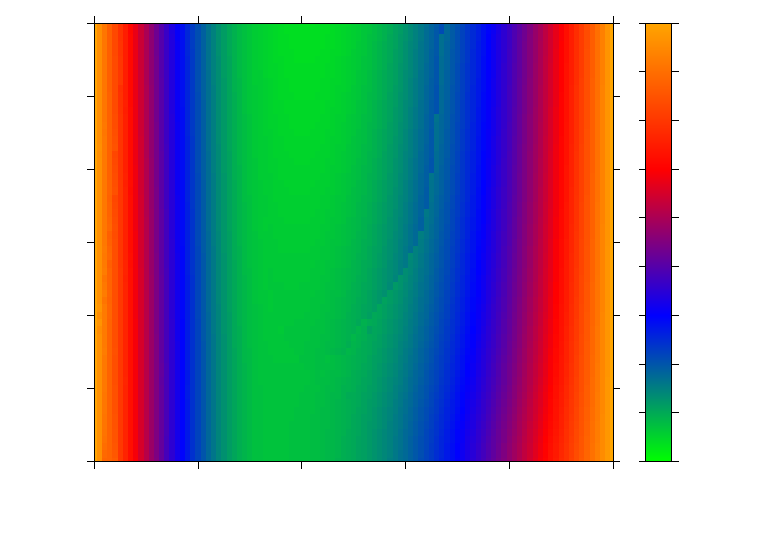
\includegraphics{E0depend}}%
    \gplfronttext
  \end{picture}%
\endgroup

\caption{Relative energy difference $(E_{0,2} - E_{0,1})/|E_{0,1}|$ of searching for $\Delta_k \sim \sin(2kd)$ and $\Delta_k\sim \sin(kd)$ corresponding to the diagrams in figure \ref{fig.phasediagram.t21.0}. A positive value indicates that the $\sin(kd)$-like solution is energetically favourable. Parameters: $t_2 = t_1$, $G = 4$, $N = 100$. }
\label{fig.energydifference.t21.0}
\end{center}
\end{figure}

The figure has the additional advantage that it shows us exactly in what region, we find $\Delta_k \sim \sin(2kd)$ solutions. Comparing this with figure \ref{fig.phasediagram.t21.0} we see that there is a region of the $\nu = 1$ phase, where we find $\sin(2kd)$-like solutions as mentioned above. 

In this analysis we have only studied the dominant nearest neighbour hopping regime: $t_1 \leq t_2$. However, as mentioned in section \ref{sec.TightbindingHam.lattice} it is possible to tune $t_2$ to be the dominant hopping term by appropriately shaking the optical lattice. We have briefly studied the case of vanishing nearest neighbour hopping, $t_1 = 0 \neq t_2$. The results are not altered significantly in this case.\footnote{The most important difference is that in this case there is only a $\nu = 0$ and $\nu = 2$ phase.} The dominant nearest neighbour pairing is still slightly energetically favourable.

We have also briefly studied the fermionic one-dimensional lattice in the three-dimensional Bose-Einstein condensate. For this system it is much more difficult to find the phase with winding number $\nu = 2$. This is connected to the fact that the induced interaction in this case is of the Yukawa form. Hence, even in the infinite coherence length limit, the interaction falls off as $1 / r$, $r$ being the interparticle distance between the fermions. However, for vanishing nearest neighbour hopping, $t_1 = 0$, but $t_2$ nonzero it is possible to find exact BCS mean field solutions with $\Delta_k = t_2\sin(2kd)$, if we tune the interaction strength and the coherence length in a specific way. These exact mean field solutions can both be found for the 1D-1D system investigated above and the 1D-3D system mentioned here. A calculation of the total energy of these phases shows that for the 1D-3D system the energy difference between the $\nu = 1$ phase and the desired $\nu = 2$ is almost $100 \%$. As mentioned above the energy difference in the 1D-1D system of these two phases is only a few percent. Hence, the desired phase with winding number $\nu = 2$ is much closer to the ground state with $\nu = 1$ in the 1D-1D system. This is a truly satisfactory result. 



 
% Chapter 9

\chapter{Grand Fermi Hamiltonian} % Main chapter title

\label{Chapter9} % For referencing the chapter elsewhere, use \ref{Chapter9} 

\lhead{Part III. \emph{Two wires}}
\chead{Chapter 9. \emph{Grand Fermi Hamiltonian}} % This is for the header on each page - perhaps a shortened title

%----------------------------------------------------------------------------------------
In this chapter we will study the fermion Hamiltonian. Firstly, we will make the mean field approximation analogous to the one in chapter \ref{Chapter4}. See section \ref{sec.2wiresmeanfieldapproximation}. Secondly, we will write up the grand Hamiltonian for the fermions. See section \ref{sec.2wiresgrandHFF}. Thirdly, we will derive the gap equations in section \ref{sec.2wiresgapandnumberequations}. Finally, in section \ref{sec.2wiressymmetries} we disciss the symmetries and use these to classify the grand Hamiltonian topologically. 

\section{Interaction Hamiltonian and the mean field approximation}
\label{sec.2wiresmeanfieldapproximation}
The interaction Hamiltonians for the intrawire interactions of the fermions are the same as the one studied in chapter \ref{Chapter4}. This also means, that we get analogous gap equations for the pairing potentials internally in wire 1 and 2 (see equation \ref{eq.pairingpotentialdef}) :
\begin{align}
\Delta^{11}_k &= -\frac{1}{\mathcal{L}} \sum_{k'} W_{\text{ind}}^{11}(k,k')\braket{c_{1,k'}c_{1,-k'}}, \nonumber \\
\Delta^{22}_k &= -\frac{1}{\mathcal{L}} \sum_{k'} W_{\text{ind}}^{22}(k,k')\braket{c_{2,k'}c_{2,-k'}}, \nonumber \\
W_{\text{ind}}^{11}(k,k') &= W_{\text{ind}}^{22}(k,k') = \frac{1}{2}\left[V_{\text{ind}}^{11}(k-k',0) - V_{\text{ind}}^{11}(k+k',0) \right].
\label{eq.pairingpotentialsintrawire}
\end{align}

However, this does not mean, that $\Delta^{11}_k = \Delta^{22}_k$, since $\braket{c_{1,k}c_{1,-k}}$ and $\braket{c_{2,k}c_{2,-k}}$ can potentially be different. We will return to this later on. The above pairing potentials are associated with the following terms of the total $H^\text{int}_{FF}$:
\begin{align}
H^\text{int}_{FF,11} &= \frac{1}{2}\sum_k \left[\Delta^{11}_k c^\dagger_{1,k}c^\dagger_{1,-k} + \Delta^{11 *}_k c_{1,-k}c_{1,k} - \Delta^{11}_k\braket{c^\dagger_{1,k}c^\dagger_{1,-k}} \right], \nonumber \\
H^\text{int}_{FF,22} &= \frac{1}{2}\sum_k \left[\Delta^{22}_k c^\dagger_{2,k}c^\dagger_{2,-k} + \Delta^{11 *}_k c_{2,-k}c_{2,k} - \Delta^{22}_k\braket{c^\dagger_{2,k}c^\dagger_{2,-k}} \right].
\label{eq.Hintintrawire}
\end{align}

The interaction Hamiltonian for the interwire interaction is:
\begin{equation}
H^\text{int}_{FF,12} = \int dx_1 dx_2 \psi^\dagger_{1,F}(x_1)\psi^\dagger_{2,F}(x_2) \tilde{V}_{\text{ind}}^{12}(x_1-x_2,0) \psi_{2,F}(x_2)\psi_{1,F}(x_1).
\label{eq.Hint12realspace}
\end{equation}
The factor in front of $1/2$ is absent, since the fermions in wire 1 and 2 are distinguishable. By going to momentum space a little calculation shows that it can be written as:
\begin{equation}
H^\text{int}_{FF,12} = \frac{1}{\mathcal{L}}\sum_{k,q,p} V_{\text{ind}}^{12}(p,0) c^\dagger_{1,k + p} c^\dagger_{2, q - p} c_{2, q} c_{1, k}. 
\label{eq.Hint12momentumspace}
\end{equation}
The summand describes a scattering with a momentum exchange $p$ and amplitude $V_{\text{ind}}^{12}(p,0)$. As for the intrawire case we assume, that only states with opposite momentum couples. This means, that we can truncate the above sum to $q = -k$ only. Further we make a mean field approximation with the mean field $\braket{c_{2,k}c_{1,-k}}$. Writing $p = k' - k$ we hereby get:
\begin{align}
H^\text{int}_{FF,12} = \frac{1}{\mathcal{L}} \sum_{k,k'} V_{\text{ind}}^{12}(k-k',0) & \left[\braket{c_{2,k'}c_{1,-k'}}c^\dagger_{1,-k}c^\dagger_{2,k} + \braket{c^\dagger_{1,-k'}c^\dagger_{2,k'}}c_{2,k}c_{1,-k} - \braket{c_{2,k'}c_{1,-k'}}\braket{c^\dagger_{1,-k}c^\dagger_{2,k}} \right]. \nonumber
\end{align}
We therefore define the interwire pairing potential as:
\begin{equation}
\Delta^{12}_k = -\frac{1}{\mathcal{L}} \sum_{k'} V_{\text{ind}}^{12}(k-k',0)\braket{c_{2,k'}c_{1,-k'}}.
\end{equation}
This brings the interaction part of the interwire Hamiltonian on the following form:\footnote{As for the single wire, this is technically no longer an interaction Hamiltonian, since it is only quadratic in the operators.}
\begin{equation}
H^\text{int}_{FF,12} = \sum_{k} \left[\Delta^{12}_k c^\dagger_{2,k}c^\dagger_{1,-k} + \Delta^{12 *}_k c_{1,-k}c_{2,k} - \Delta^{12}_k\braket{c^\dagger_{2,k}c^\dagger_{1,-k}} \right].
\label{eq.Hintinterwire}
\end{equation}
Equations \ref{eq.Hintintrawire} and \ref{eq.Hintinterwire} are the essential equations for the following. 

\section{Grand Hamiltonian}
\label{sec.2wiresgrandHFF}
The grand fermion Hamiltonian is obtained in a similar manner to the single wire analog. The free fermion part is now: $H_{0,1}+H_{0,2} = \sum_{j,k}\frac{k^2}{2m_F}c^\dagger_{j,k}c_{j,k}$. Further, the Hamiltonian is not particle number conserving, since it contains terms like $c^\dagger c^\dagger$. In stead we impose diffusive equilibrium by subtracting $\mu_1N_{1,F}+\mu_2N_{2,F}$. $\mu_j$ is the chemical potential of wire $j$ and $N_{j,F} = \sum_k c^\dagger_{j,k}c_{j,k}$ is the number of $j$ fermions. We hereby get the following grand Hamiltonian:
\begin{align}
H_{FF} = &\sum_j \left[H_{0,j} - \mu_j N_{j,F}\right] + H^\text{int}_{FF,11} + H^\text{int}_{FF,22} + H^\text{int}_{FF,12} \nonumber \\
       = &\frac{1}{2}\sum_k C^\dagger_k \mathcal{H}_{FF,k}C_k + \frac{1}{2}\sum_k\left[\varepsilon_{1,k} + \varepsilon_{2,k} - \Delta^{11}_k\braket{c^\dagger_{1,k}c^\dagger_{1,-k}} - \Delta^{22}_k\braket{c^\dagger_{2,k}c^\dagger_{2,-k}} - 2\Delta^{12}_k\braket{c^\dagger_{2,k}c^\dagger_{1,-k}} \right], \nonumber
\end{align}

with:
\begin{equation}
\mathcal{H}_{FF,k} = \begin{bmatrix} \varepsilon_{1,k} & \Delta^{11}_k      & 0                 & -\Delta^{12}_{-k} \\ 
                                     \Delta^{11 *}_k   & -\varepsilon_{1,k} & \Delta^{12*}_k    & 0 \\ 
                                    0                  & \Delta^{12}_k      & \varepsilon_{2,k} & \Delta^{22}_k \\ 
                                     -\Delta^{12*}_{-k}& 0                  & \Delta^{22*}_k    & -\varepsilon_{2,k} \end{bmatrix}, \hspace{0.5cm}
C_k =  \begin{bmatrix} c_{1,k} \\ c^\dagger_{1,-k} \\ c_{2,k} \\ c^\dagger_{2,-k} \end{bmatrix}.                                     
\end{equation}
Here $\varepsilon_{j,k} = \frac{k^2}{2m_F}-\mu_j$ is the kinetic energy relative to the chemical potential of the $j$ fermions. This has a quite general structure. To simplify matters we firstly assume, that the wires are held at the same chemical potential $\mu$. Hence we let $\varepsilon_{j,k} \to \varepsilon_k$. Secondly, we make two separate gauge transformations to make the intrawire pairings, $\Delta^{jj}_k$, real. Since the chemical potentials of the two wires is now the same, the two wires are equivalent. Hence, the system is symmetric in the 1 and 2 fermions. This means, that the pairings must be equal up to an overall phase: $\Delta^{22}_k = \text{e}^{i\phi} \Delta^{11}_k$. Since they are now real we can obtain the relation: $\Delta^{22}_k = -\Delta^{11}_k$. The overall sign difference is chosen, since it makes the eigenvectors to $\mathcal{H}_{FF,k}$ a bit simpler. The interwire pairing $\Delta^{12}_k$ describes a pairing between distinguishable particles. If we think of the wires as indexed with a pseudospin, the pairing is expected to be a $s$-wave type pairing. We will therefore search for an even solution for $\Delta^{12}_k$. This means, that:
\begin{equation}
\mathcal{H}_{FF,k} = \begin{bmatrix} \varepsilon_{k}   & \Delta^{11}_k      & 0                 & -\Delta^{12}_{k} \\ 
                                     \Delta^{11}_k     & -\varepsilon_{k}   & \Delta^{12*}_k    & 0 \\ 
                                    0                  & \Delta^{12}_k      & \varepsilon_{k}   & -\Delta^{11}_k \\ 
                                     -\Delta^{12*}_{k} & 0                  & -\Delta^{11}_k     & -\varepsilon_{k} \end{bmatrix},                  
\end{equation}
We have hereby specified two global phases. Since this is the total gauge freedom of the Hamiltonian, this means that the phase of $\Delta^{12}_k$ must be held completely general for the time being. As for the single wire the eigenvalues of the kernel above come in plus/minus pairs. The norm of the eigenvalues give the energy dispersion. The result is:
\begin{equation}
E^{\pm}_{F,k} = \sqrt{\varepsilon^2_k + \left(\Delta^{11}_k\right)^2 + \left|\Delta^{12}_k\right|^2 \pm \Delta^{11}_k(\Delta^{12}_k + \Delta^{12*}_k)}. 
\end{equation} 
This shows, that the excitation energies depends on the phase of the interwire pairing, $\Delta^{12}_k$. Since $\Delta^{11}_k$ is odd in $k$ and and $\Delta^{12}_k$ is even in $k$, we get that $E^{+}_{F,k} = E^{-}_{F,-k}$. Notice, that due to the presence of $\pm \Delta^{11}_k(\Delta^{12}_k + \Delta^{12*}_k)$ in $E^{\pm}_{F,k}$, the dispersions are neither even nor odd in $k$. If one is bothered by this, it is possible to redefine the eigenvalues to $\bar{E}^{\pm}_{F,k} = \sqrt{\varepsilon^2_k + \left(\Delta^{11}_k\right)^2 + \left|\Delta^{12}_k\right|^2 \pm |\Delta^{11}_k(\Delta^{12}_k + \Delta^{12*}_k)|}$, which are manifestly even in $k$. This is a basic reshuffling of the eigenvalues. The eigenvectors are however much more involved, and in turn the derivation of the gap equations is more cumbersome. The result in the end is the same however, and therefore we will stick to the above energy eigenvalues.  

The new quasiparticle operators are found by finding the eigenvectors to $\mathcal{H}_{FF,k}$. We define the quasiparticle fermionic operators $\gamma_{j,k}$ by:
\begin{equation}
\begin{bmatrix} c_{1,k} \\ c^\dagger_{1,-k} \\ c_{2,k} \\ c^\dagger_{2,-k} \end{bmatrix} = U_{F,k}\begin{bmatrix} \gamma_{1,k} \\ \gamma^{\dagger}_{1,-k} \\ \gamma_{2,k} \\ \gamma^{\dagger}_{2,-k} \end{bmatrix}.
\label{eq.zetaoperatorstwowiresdefinition}
\end{equation} 
The $\gamma$ operators have to obey the same anticommutation relations as the $c$ operators. Specifically all anticommutators between 1 and 2 quasiparticles, like $\{\gamma_1, \gamma_2 \} $, vanishes. $\mathcal{H}_{FF,k}$ should then be diagonalised to yield:
\begin{equation}
U^\dagger_{FF,k}\mathcal{H}_{FF,k}U_{FF,k} = \begin{bmatrix} 
E^{-}_{F,k} & 0        & 0       & 0        \\ 
0       & -E^{-}_{F,-k} & 0       & 0        \\ 
0       & 0        & E^{+}_{F,k} & 0        \\ 
0       & 0        & 0       & -E^{+}_{F,-k} \\ 
\end{bmatrix} = \begin{bmatrix} 
E^{-}_{F,k} & 0        & 0       & 0        \\ 
0       & -E^{+}_{F,k} & 0       & 0        \\ 
0       & 0        & E^{+}_{F,k} & 0        \\ 
0       & 0        & 0       & -E^{-}_{F,k} \\ 
\end{bmatrix} \nonumber
\end{equation}
Further the diagonalisation must respect the symmetry in the 1 and 2 fermions of the Hamiltonian. Specifically the assumption of $\Delta^{22}_k = -\Delta^{11}_k$ must be selfconsistent. From equation \ref{eq.pairingpotentialsintrawire} this means, that $\braket{c_{2,k}c_{2,-k}} = -\braket{c_{1,k}c_{1,-k}}$. Finally, since the elements of $C_k$ are not independent, we get some internal structure of $U_{F,k}$. Let us write the elements of $U_{F,k}$ as $u^{ij}_k$. From equation \eqref{eq.zetaoperatorstwowiresdefinition} we take the first row and the conjugate of the second row with $-k \to k$:
\begin{align}
c_{1,k} &= u^{11}_k \gamma_{1,k} + u^{12}_k \gamma^\dagger_{1,-k} + u^{13}_k \gamma_{2,k} + u^{14}_k \gamma^\dagger_{2,-k}, \nonumber \\
c_{1,k} &= u^{22*}_{-k} \gamma_{1,k} + u^{21*}_{-k} \gamma^\dagger_{1,-k} + u^{24*}_{-k} \gamma_{2,k} + u^{23*}_{-k} \gamma^\dagger_{2,-k}. \nonumber
\end{align}
Since the coefficients in front of e.g. $\gamma_{1,k}$ must be the same in both expressions, we get that $u^{11}_k = u^{22*}_{-k}$. This means, that $U_{F,k}$ has the following structure due to the built-in particle-hole symmetry:
\begin{equation}
U_{F,k} = \begin{bmatrix} 
u^{22*}_{-k} & u^{21*}_{-k} & u^{24*}_{-k} & u^{23*}_{-k}           \\  
u^{21}_k 	 & u^{22}_k 	& u^{23}_k 	   & u^{24}_k               \\ 
u^{42*}_{-k} & u^{41*}_{-k} & u^{44*}_{-k} & u^{43*}_{-k}           \\ 
u^{41}_k 	 & u^{42}_k 	& u^{43}_k 	   & u^{44}_k
\end{bmatrix}. \nonumber
\end{equation}
Now define the norms $A^{\pm}_k = 2 \sqrt{ E^{\pm}_{F,k}(\varepsilon_k + E^{\pm}_{F,k}) }$. With a bit of trial and error the above requirements combined result in:
\begin{equation}
U_{F,k} = \begin{bmatrix} 
\frac{\varepsilon_k + E^{-}_{F,k}}{A^{-}_k}    & -\frac{\Delta^{11}_k + \Delta^{12}_k}{A^{+}_k} & \frac{\varepsilon_k + E^{+}_{F,k}}{A^{+}_k}     & -\frac{\Delta^{11}_k - \Delta^{12}_k}{A^{-}_k}  \\  
\frac{\Delta^{11}_k - \Delta^{12*}_k}{A^{-}_k} & \frac{\varepsilon_k + E^{+}_{F,k}}{A^{+}_k}    & \frac{\Delta^{11}_k + \Delta^{12*}_k}{A^{+}_k}  & \frac{\varepsilon_k + E^{-}_{F,k}}{A^{-}_k}     \\ 
-\frac{\varepsilon_k + E^{-}_{F,k}}{A^{-}_k}   & -\frac{\Delta^{11}_k + \Delta^{12}_k}{A^{+}_k} & \frac{\varepsilon_k + E^{+}_{F,k}}{A^{+}_k}     & \frac{\Delta^{11}_k - \Delta^{12}_k}{A^{-}_k} \\ 
\frac{\Delta^{11}_k - \Delta^{12*}_k}{A^{-}_k} & -\frac{\varepsilon_k + E^{+}_{F,k}}{A^{+}_k}   & -\frac{\Delta^{11}_k + \Delta^{12*}_k}{A^{+}_k} & \frac{\varepsilon_k + E^{-}_{F,k}}{A^{-}_k} 
\end{bmatrix}. \nonumber
\end{equation}
The diagonalisation of the Hamiltonian is now straight forward. $U^\dagger_{F,k}\mathcal{H}_{FF,k}U_{F,k}$ is diagonal with the eigenvalues $+E^{\pm}_{F,k}$ and $-E^{\pm}_{F,k}$ alternating in the diagonal as shown above. The result of the diagonalisation is therefore:
\begin{align}
H_{FF} &= E_0 + \sum_{k} \left[ E^{-}_{F,k}\gamma^\dagger_{1, k}\gamma_{1, k} + E^{+}_{F,k}\gamma^\dagger_{2, k}\gamma_{2, k} \right], \nonumber \\ 
E_0 &= \frac{1}{2}\sum_k \left[2\varepsilon_k - \left( E^{-}_{F,k} + E^{+}_{F,k} + \Delta^{11}_k\braket{c^\dagger_{1,k}c^\dagger_{1,-k}} + \Delta^{22}_k\braket{c^\dagger_{2,k}c^\dagger_{2,-k}} + 2\Delta^{12}_k\braket{c^\dagger_{2,k}c^\dagger_{1,-k}} \right) \right]. 
\label{eq.2wiresDiagonalisedHamiltonian}
\end{align}  
Analogously to the single wire case the ground state is hereby defined by $\gamma_{j,k}\ket{\text{S}}_0 = 0$ for $j = 1, 2$. The ground state \textit{grand} energy $E_0$ is derived similarly to the gap equations of the next section. Using the found diagonalisation matrix $U_{F,k}$, we express the $c$-operators in terms of $\gamma$-operators and use, that the $\gamma$-operators obey Fermi statistics: $\braket{\gamma^\dagger_{1,k}\gamma_{1,k}} = f(E^{-}_{F,k})$, and $\braket{\gamma^\dagger_{2,k}\gamma_{2,k}} = f(E^{+}_{F,k})$, with $f(E) = (\text{e}^{\beta E} + 1)^{-1}$ the Fermi-Dirac distribution. For $T=0$ the expression is particularly simple. We get:
\begin{equation}
\frac{E_0}{\epsilon_{F,0} N_F} = -\frac{1}{4} \int d\tilde{k} \frac{(\tilde{\varepsilon}_{\tilde{k}} - \tilde{E}^{+}_{F, \tilde{k}})^2}{\tilde{E}^{+}_{F, \tilde{k}}}, \hspace{0.5cm} T = 0. 
\label{eq.2wiresGrandGroundStateEnergy}
\end{equation}
We have expressed the momentum as $\tilde{k} = k/k_F$, and the energies as $\tilde{E} = E/\epsilon_{F,0}$. We notice, that the ground state grand energy is negative. This is because, we are measuring energies with respect to the chemical potential. The motivation for calculating the grand energy is the following. For any temperature the grand energy, $\Phi$, is given by $\Phi = U - TS - 2\mu N_F = F - 2\mu N_F$, where $F$ is the Helmholtz free energy \cite[pp. 161-162]{SchroederThermal}. The presence of the factor of 2 is simply because there are $N_F$ fermions in \textit{each} wire. Physically, we hold the number of particles fixed. This means, that it is the Helmholtz free energy $F = \Phi + 2\mu N_F$ we have to minimize to find the preferred state, not $\Phi$. For $T = 0$, this means, that the energetically favourable state is the one, that exhibits a minimum of $F(T = 0) = E_0 + 2\mu N_F$. The aim is therefore to calculate the Helmholtz free energy for differing phases of $\Delta^{12}_k$ and see which one is the lowest. 

\section{Gap and number equations}
\label{sec.2wiresgapandnumberequations}
In this section we write up and discuss the gap equations. They are derived in complete analogy to the single wire case and in the same way as the ground state energy of the previous section. The gap equations hereby become:
\begin{align}
\Delta^{11}_k &= -\frac{1}{\mathcal{L}}\sum_{k'} W_{\text{ind}}^{11}(k, k')\frac{\Delta^{11}_{k'} + \Delta^{12}_{k'}}{2E^{+}_{F,k'}}\tanh\left[\frac{\beta E^{+}_{F,k'}}{2}\right], \nonumber \\
\Delta^{12}_k &= -\frac{1}{\mathcal{L}}\sum_{k'} W_{\text{ind}}^{12}(k, k')\frac{\Delta^{12}_{k'} + \Delta^{11}_{k'}}{2E^{+}_{F,k'}}\tanh\left[\frac{\beta E^{+}_{F,k'}}{2}\right].
\label{eq.2wiresgapequations}
\end{align}
We further get that $\Delta^{22}_k = - \Delta^{11}_k$, so that this assumption is self-consistent. Notice, that the two equations have the exact same structure. This is achieved by defining the effective \textit{inter}wire interaction: 
\begin{equation}
W_{\text{ind}}^{12}(k, k') = \frac{1}{2}\left[V_{\text{ind}}^{12}(k - k', 0) + V_{\text{ind}}^{12}(k + k', 0) \right].
\end{equation}
This is seen to be quite analogous to the \textit{intra}wire effective interaction $W_{\text{ind}}^{11}(k, k')$. The induced interaction $V_{\text{ind}}^{12}(q, 0)$ only depends on $q^2$. This gives us the following symmetry properties of the effective interaction:
\begin{align}
W_{\text{ind}}^{12}(k,k')   &= W_{\text{ind}}^{12}(k',k), \hspace{0.5cm} \text{Symmetry in arguments}, \nonumber \\
W_{\text{ind}}^{12}(-k,k')  &= W_{\text{ind}}^{12}(k,k'), \hspace{0.5cm} \text{Even in arguments}.
\label{eq.EffectiveInterwireInteractionSymmetries}
\end{align}
This is very similar to the symmetry properties of $W_{\text{ind}}^{11}(k, k')$ listed in equation \ref{eq.EffectiveInteractionSymmetries}, with the only difference, that the interwire effective interaction defined here is even in a single argument. We notice, that these gap equations have a slightly different structure than the ones for the single wire. Finally, the above quations goes to the gap equations for the separated single wires found in chapter \ref{Chapter4}, when $\Delta^{12}_k$ goes to $0$.   	

It turns out that the number equation calculated from $N_F = \sum_k \braket{c^\dagger_{j,k}c_{j,k}}$ has the exact same structure as the single wire number equation. Explicitly: 
\begin{equation}
n_F = \frac{1}{2}\int \frac{dk}{2\pi} \left( 1 - \frac{\varepsilon_k}{E^{+}_{F,k}}\tanh\left[\frac{\beta E^{+}_{F,k}}{2}\right] \right). 
\label{eq.2wiresnumberequation}
\end{equation}
Taking the real part of the first gap equation and the real and imaginary part of the second one together with the number equation gives us four equations for the four quantitites $\Delta^{11}_k, \Delta^{12}_{k,r}, \Delta^{12}_{k,i} $ and $\mu$. Here we write the interwire pairing as decomposed in its real and imaginary parts: $\Delta^{12}_k = \Delta^{12}_{k,r} + i\Delta^{12}_{k,i}$. Finally, taking the imaginary part of the first gap equation gives a fifth self-consistency equation:
\begin{equation}
0 = -\frac{1}{\mathcal{L}}\sum_{k'} W_{\text{ind}}^{11}(k, k')\frac{\Delta^{12}_{k',i}}{2E^{+}_{F,k'}}\tanh\left[\frac{\beta E^{+}_{F,k'}}{2}\right].
\end{equation}
This equation has two trivial solutions. The first is, where the interwire pairing is real. Then the integrand is 0 and the equation is fulfilled. The second is, where the interwire pairing is purely imaginary. Then the two dispersion relations are identical: $E^{\pm}_{F,k} = \sqrt{\varepsilon_k^2 + (\Delta^{11}_k)^2 + |\Delta^{12}_k|^2}$. Then the summand is in total an odd function in $k'$ and so the equation is again fulfilled. We will only investigate these two cases, because they exhibit interesting symmetries of the system. This is discussed in the following section.

\section{Symmetries}
\label{sec.2wiressymmetries}
\subsection{Time reversal symmetries with wire exchange}
\label{subsec.TRwireexchange}
In this subsection we will show, that we can construct two types of time reversal symmetries of the system, that exchange the wires. One is obeyed if the interwire pairing is imaginary; this squares to $+\mathbb{I}$. The other is obeyed if the interwire pairing is real; this squares to $-\mathbb{I}$. We will further shortly discuss the particle-hole and sublattice symmetries, and finally how these symmetries puts the Hamiltonian in a specific symmetry class. 

We first define a time reversal operator, that squares to $\mathbb{I}$ and interchanges the wires: 
\begin{equation}
T_+\begin{bmatrix} c^\dagger_{1,k} \\ c^\dagger_{2,k} \end{bmatrix} T_+^{-1} = \eta\sigma_1 \begin{bmatrix} c^\dagger_{1,-k} \\ c^\dagger_{2,-k} \end{bmatrix} = \eta\begin{bmatrix} c^\dagger_{2,-k} \\ c^\dagger_{1,-k} \end{bmatrix},\nonumber
\end{equation} 
with $\sigma_1$ the first Pauli matrix operating in wire space and $\eta$ some overall phase. Hence, under this time reversal transformation a fermion from wire 1 is transformed into a fermion in wire 2 and acquires the phase $\eta$. Since $(\eta\sigma_1)(\eta\sigma_1)^* = \sigma_1^2 = \mathbb{I}$ we get, that $T_+$ squares to plus the identity. The question is now, under what circumstances $T_+$ is a symmetry of the Hamiltonian. Since $\varepsilon_{1,k} = \varepsilon_{2,k}$, the only problematic terms under time reversal are $\Delta^{11}_k c^\dagger_{1,k}c^\dagger_{1,-k}, \Delta^{22}_k c^\dagger_{2,k}c^\dagger_{2,-k}$ and $\Delta^{12}_kc^\dagger_{2,k}c^\dagger_{1,-k}$. We remember, that time reversal is antiunitary: $TiT^{-1} = -i$. This means, that the first transform according to:
\begin{equation}
\Delta^{11}_k c^\dagger_{1,k}c^\dagger_{1,-k} \overset{T_+}{\to} \Delta^{11*}_k \left(\eta c^\dagger_{2,-k}\right)\left(\eta c^\dagger_{2,k}\right) = -\eta^2\Delta^{11}_k c^\dagger_{2,k}c^\dagger_{2,-k}. \nonumber
\end{equation}
Here we use, that $\Delta^{11}_k$ is chosen to be real. This term should be identical to the original term connected to the product $c^\dagger_{2,k}c^\dagger_{2,-k}$: $\Delta^{22}_k c^\dagger_{2,k}c^\dagger_{2,-k}$. Since, we have chosen the intrawire pairings real and with an overall sign difference, we see, that we need $\eta^2 = 1$. Hence $\eta = \pm 1$ is required. The transformation of $\Delta^{22}_k c^\dagger_{2,k}c^\dagger_{2,-k}$ leads to the same result. Further:
\begin{equation}
\Delta^{12}_k c^\dagger_{2,k}c^\dagger_{1,-k} \overset{T_+}{\to} \Delta^{12*}_k \left(\eta c^\dagger_{1,-k}\right)\left( \eta c^\dagger_{2,k}\right) = -\eta^2 \Delta^{12*}_k c^\dagger_{2,k}c^\dagger_{1,-k} = - \Delta^{12*}_k c^\dagger_{2,k}c^\dagger_{1,-k}. \nonumber
\end{equation}
This shows, that independent of $\eta$, we need $\Delta^{12*}_k = - \Delta^{12}_k$. Hence, the interwire pairing must be imaginary to obey this time reversal symmetry.\footnote{Had we chosen the phases of the intrawire pairings differently we could ensure a time reversal symmetry by changing the overall phase acquired under $T_+$.} As in section \ref{sec.SymmetriesTRandPH} we can convert the second quantized operator to one in first quantization:
\begin{equation}
\mathcal{T}_+ = \sigma_1\otimes \tau_0 \cdot K, 
\label{eq.2wiresTpluswireexchangefirstquantization}
\end{equation}
where $K$ is the complex conjugation operator and $\tau_i$ are the Pauli matrices operating in particle-hole space. Here we have chosen $\eta = 1$. The symmetry is then described by the fact that: $\mathcal{T}_+\mathcal{H}_{FF,k} = \mathcal{H}_{FF,-k}\mathcal{T}_+$.

We now define a time reversal operator, that squares to $-\mathbb{I}$ and interchanges the wires:
\begin{equation}
T_-\begin{bmatrix} c^\dagger_{1,k} \\ c^\dagger_{2,k} \end{bmatrix} T_-^{-1} = \eta\sigma_2 \begin{bmatrix} c^\dagger_{1,-k} \\ c^\dagger_{2,-k} \end{bmatrix} = -i\eta\begin{bmatrix} c^\dagger_{2,-k} \\ - c^\dagger_{1,-k} \end{bmatrix}.\nonumber
\end{equation} 
This transformation is different from $T_+$ in the sense, that there is an overall sign difference in the transformation of the two types of fermions. Since $(\eta \sigma_2)(\eta \sigma_2)^* = \sigma_2\sigma_2^* = - \sigma_2^2 = - \mathbb{I}$, this time reversal operator squares to minus the identity. Again we ask under what conditions this is a symmetry of the Hamiltonian. Looking at the same terms as before, we firstly get:
\begin{equation}
\Delta^{11}_k c^\dagger_{1,k}c^\dagger_{1,-k} \overset{T_-}{\to} \Delta^{11*}_k \left(-i\eta c^\dagger_{2,-k}\right)\left(-i\eta c^\dagger_{2,k}\right) = \eta^2\Delta^{11}_k c^\dagger_{2,k}c^\dagger_{2,-k}. \nonumber
\end{equation}
This term should be identical to the original term connected to the product $c^\dagger_{2,k}c^\dagger_{2,-k}$: $\Delta^{22}_k c^\dagger_{2,k}c^\dagger_{2,-k}$. We hereby see, that we need $\eta = \pm i$. Further:
\begin{equation}
\Delta^{12}_k c^\dagger_{2,k}c^\dagger_{1,-k} \overset{T_-}{\to} \Delta^{12*}_k \left(i\eta c^\dagger_{1,-k}\right)\left(-i\eta c^\dagger_{2,k}\right) = -\eta^2 \Delta^{12*}_k c^\dagger_{2,k}c^\dagger_{1,-k} = \Delta^{12*}_k c^\dagger_{2,k}c^\dagger_{1,-k}. \nonumber
\end{equation}
This shows, that independent of $\eta$, we need $\Delta^{12*}_k = \Delta^{12}_k$. Hence, the interwire pairing must be real to obey this time reversal symmetry. In first quantization we can express this time reversal operator as:
\begin{equation}
\mathcal{T}_- = i\sigma_2\otimes\tau_0 \cdot K, 
\label{eq.2wiresTminuswireexchangefirstquantization}
\end{equation}
where again $\sigma_i, \tau_i$ are Pauli matrices operating in wire and particle-hole space respectively. 

Similarly to the single wire case we can define a particle-hole transformation, that effectively does not change the spinor $C_k$, since the Hamiltonian of this two wire system is still of the Bogoliubov-de Gennes type. Explicitly we let:
\begin{equation}
C\begin{bmatrix} c_{j,k} \\ c^\dagger_{j,-k} \end{bmatrix}C^{-1} = \tau_1 \begin{bmatrix} c^\dagger_{j,-k} \\ c_{j,k} \end{bmatrix} = \begin{bmatrix} c_{j,k} \\ c^\dagger_{j,-k} \end{bmatrix}, 
\end{equation} 
both for $j=1$ and $j=2$. It is then clear, that the total spinor $C_k$ is also unaffected by the transformation. As a result the Hamiltonian is invariant under $C$, and $\tau_1^2 = \mathbb{I}$ so the transformation squares to unity. 

This analysis also gives us a sublattice symmetry in the case of an imaginary or real interwire pairing: $S_\pm = T_\pm C$. In total this puts the system in Cartan class BDI, if $\Delta^{12}_k$ is imaginary, and in Cartan class DIII, if $\Delta^{12}_k$ is real. The topological index is respectively to be found in the integers $\mathbb{Z}$ and in $\mathbb{Z}_2 = \{-1,1\}$. See table \ref{tab.PeriodicTableTISC} for the details. We will return to the actual determination of these invariants in chapter \ref{Chapter10}. 

\subsection{Time reversal symmetries with separate wires} 
\label{subsec.TRseparatewires}
In this subsection we will show, that the system has yet another two time reversal symmetries. These keep the wires separated and both square to $+\mathbb{I}$. 

There are two possibilities for this symmetry: 
\begin{equation}
T_1 \begin{bmatrix} c^\dagger_{1,k} \\ c^\dagger_{2,k} \end{bmatrix} T_1^{-1} = \eta\sigma_0 \begin{bmatrix} c^\dagger_{1,-k} \\ c^\dagger_{2,-k} \end{bmatrix} = \eta\begin{bmatrix} c^\dagger_{1,-k} \\ c^\dagger_{2,-k} \end{bmatrix}, \hspace{0.5cm} T_2 \begin{bmatrix} c^\dagger_{1,k} \\ c^\dagger_{2,k} \end{bmatrix} T_2^{-1} = \eta\sigma_3 \begin{bmatrix} c^\dagger_{1,-k} \\ c^\dagger_{2,-k} \end{bmatrix} = \eta\begin{bmatrix} c^\dagger_{1,-k} \\  - c^\dagger_{2,-k} \end{bmatrix}. \nonumber
\end{equation} 
It is evident, that both symmetries square to $+\mathbb{I}$. For both of them we get: 
\begin{equation}
\Delta^{11}_k c^\dagger_{1,k}c^\dagger_{1,-k} \overset{T_j}{\to} \Delta^{11*}_k \left(\eta c^\dagger_{1,-k}\right)\left(\eta c^\dagger_{1,k}\right) = -\eta^2\Delta^{11}_k c^\dagger_{1,k}c^\dagger_{1,-k}, \nonumber
\end{equation}
since $\Delta^{11}_k$ is chosen real. This shows, that we must have $\eta^2 = -1$. The relevant terms containing $\Delta^{12}_k$ transform according to:
\begin{equation}
\sum_k \Delta^{12}_k c^\dagger_{2,k}c^\dagger_{1,-k} \overset{T_j}{\to} \sum_k \Delta^{12*}_k \left(\pm \eta c^\dagger_{2,-k}\right)\left( \eta c^\dagger_{1,k}\right) = \mp \sum_k \Delta^{12*}_{k} c^\dagger_{2,k}c^\dagger_{1,-k}. \nonumber
\end{equation}
The last equality is achieved by going from $k$ to $-k$ in the sum, using that $\Delta^{12}_k$ is even in $k$, and that $\eta^2 = -1$. This shows, that both $\Delta^{12}_k$ real and imaginary realises a time reversal symmetry, which does not exchange the wires. Further, these both square to $+\mathbb{I}$.

The symmetries found in this subsection are the same as the one found for the single wire. See section \ref{sec.SymmetriesTRandPH} for the details. This shows, that the real and imaginary interwire pairing does not break the time reversal symmetry internally in each wire. Specifically, this shows that one can have both a $T^2 = +\mathbb{I}$ and $T^2 = -\mathbb{I}$ symmetry for the same system. In the present case $T_-$ and $T_2$ for $\Delta^{12}_k$ real. This might seem a little confusing at first sight, because as discussed in chapter \ref{Chapter7} the symmetries put the system in a specific Cartan class. However, the Cartan classes are not distinct in this sense per se. Rather one should think of the classification in the following sense. For the case at hand we can both put the Hamiltonian in class BDI and DIII, corresponding to $T^2 = +\mathbb{I}$ and $T^2=-\mathbb{I}$ respectively. This means, that we can ask what ground states are topologically distinct, if we preserve just one of these symmetries. Hence, the system is characterized by having \textit{two} topological indices in this case, one in $\mathbb{Z}$ and one in $\mathbb{Z}_2 = \{-1,1\}$.



% Chapter 10

\chapter{Two wires, cross over and numerical results} % Main chapter title

\label{Chapter10} % For referencing the chapter elsewhere, use \ref{Chapter9} 

\lhead{Chapter 10. \emph{2 wires, cross over \& numerical analysis}} % This is for the header on each page - perhaps a shortened title

%----------------------------------------------------------------------------------------
In this chapter we present the numerical analysis and results of the two wire system. The most noticeable of the results is, that we are able to find an interval of interwire distances, where both $s$- and $p$-wave type pairings exist, and that this is the energetically favourable state of the system.

\section{Cross over region and energy considerations}
In this section we will show numerically, that during the transition from interwire to intrawire pairing the energetically favourable state of the system is the one where the interwire pairing is purely imaginary. We will further show, that this transition is characterized by having both the interwire and intrawire pairing simultaneously nonzero over an interval of interwire distances, $d$. 

We first come with an energy analysis as described after equation \eqref{eq.2wiresGrandGroundStateEnergy}. Let us first calculate the free energy, when the two wires are just free fermion gases. For $T = 0$ the free energy is simply the sum of the kinetic energy $\frac{k^2}{2m_F}$ for $|k| < k_F$: 
\begin{equation}
F = 2\sum_{k, |k| < k_F} \frac{k^2}{2m_F} = \frac{\mathcal{L}}{\pi} \int^{k_F}_{-k_F} dk \frac{k^2}{2m_F} = \epsilon_{F,0} N_F \int^{1}_{-1} d\tilde{k}\; \tilde{k}^2 = \frac{2}{3}\epsilon_{F,0} N_F. 
\end{equation}

Now the numerical analysis. Common for all the analyses we do the following. We start at low values of $d$. First, we come with an initial guess for the pairings and the chemical potential. Second, the pairings and chemical potentials are inserting in the gap equations \ref{eq.2wiresgapequations} and an updated version of the pairings is obtained. Third, this is inserted into the number equation \ref{eq.2wiresnumberequation}, which gives an updated version of the chemical potential. Finally, this is iterated until the pairings are not altered by more than $0.1$\textperthousand. For each step of $d$ we then return to the same initial guess for the pairings to avoid any hysteresis in the analysis. We then use equation \eqref{eq.2wiresGrandGroundStateEnergy} to calculate the grand energy, $E_0$, and in turn the Helmholtz free energy $E_0 + 2\mu N_F$.  

If we let $\Delta^{12}_k = 0$ and search for nonzero $\Delta^{11}_k$ we get the dashed curve in figure \ref{fig.2wiresE0ddepend} for the specified set of parameters. Hence, this describes the situation where we only have intrawire pairing. It is independent of $d$ as it should be. Conversely, we can let $\Delta^{11}_k = 0 = \Delta^{22}_k$ and search for nonzero $\Delta^{12}_k$. This results in the dash-dotted curve. As we expect, these two curves intersect at some critical distance $d_c$. In the present case $k_Fd_c \approx 0.748$. The naively expected behaviour is then the following. For large distances, $d$, the intrawire pairing is energetically favourable and is therefore the only one present. As we decrease $d$ we get to the critical point $d_c$, where the interwire pairing becomes favourable in stead. For $d < d_c$ we would then expect the interwire pairing to be the only one present. This turns out to be the exact behaviour, if we force the interwire pairing to be real. The two types of pairings do not coexist, a sudden flip from one to the other occures. This is the blue curve in figure \ref{fig.2wiresE0ddepend}. 

The question now is: can we find a solution, where both pairings are present simultaneously and is this energetically favourable? The answer is the following. If we let $\Delta^{12}_k$ be purely imaginary and search for both nonzero $\Delta^{12}_k$ and $\Delta^{11}_k$, we get the red curve. This curve clearly represents the energetically favourable solution. Since the sudden flip between the two types of pairings is associated with the blue curve, the red curve must describe a coexistence of the two types of pairings. This we verify explicitly in the following analysis. 

For $\Delta^{12}_k$ real the analysis is performed in the same way as in the above. Only we record the maximal values $\max_k\left[\left|\Delta^{11}_k\right|\right]$ and $\max_k\left[\left|\Delta^{12}_k\right|\right]$ as a function of $d$. This results in the blue curves in figure \ref{fig.2wiresMaximalPairingddepend}. The behaviour is largely as described above. When we increase $d$ the interwire pairing decreases, until we reach the critical distance $d_c$ where it suddenly flips to a intrawire pairing in stead. 

Now let us concentrate on the energetically favourable solution: $\Delta^{12}_k$ imaginary. In this case the energy dispersions are identical and even in $k$: $E^{\pm}_{F,k} = E_{F,k} = \sqrt{\varepsilon_k^2 + (\Delta^{11}_k)^2 + |\Delta^{12}_k|^2}$. This means, that the gap equations in \eqref{eq.2wiresgapequations} partially decouples: 
\begin{align}
\Delta^{11}_k &= -\frac{1}{\mathcal{L}}\sum_{k'} W^\text{ind}_{FF,11}(k, k')\frac{\Delta^{11}_{k'}}{2E_{F,k'}}\tanh\left(\frac{\beta E_{F,k'}}{2}\right), \nonumber \\
\Delta^{12}_k &= -\frac{1}{\mathcal{L}}\sum_{k'} W^\text{ind}_{FF,12}(k, k')\frac{\Delta^{12}_{k'}}{2E_{F,k'}}\tanh\left(\frac{\beta E_{F,k'}}{2}\right).
\label{eq.2wiresgapequationsDelta12imaginary}
\end{align} 
This explicitly shows, that the two pairings are only coupled through the energy $E_{F,k}$. We start the analysis around $d = d_c$, since both pairings are suspected to be present there. For each value of $d$ we do something very similar to the above. However, here we do not reinitiate the initial guess in each step of $d$. In stead we reuse the found solution from the previous value of $d$. This makes the analysis much faster, and as long as the transition between the pairings is continuous no mistake is made. Further, we record the maximal values $\max_k\left[\left|\Delta^{11}_k\right|\right]$ and $\max_k\left[\left|\Delta^{12}_k\right|\right]$. The result is shown as the red curves in figure \ref{fig.2wiresMaximalPairingddepend}.

\begin{figure} 
\begin{center}  
% GNUPLOT: LaTeX picture with Postscript
\begingroup
  \makeatletter
  \providecommand\color[2][]{%
    \GenericError{(gnuplot) \space\space\space\@spaces}{%
      Package color not loaded in conjunction with
      terminal option `colourtext'%
    }{See the gnuplot documentation for explanation.%
    }{Either use 'blacktext' in gnuplot or load the package
      color.sty in LaTeX.}%
    \renewcommand\color[2][]{}%
  }%
  \providecommand\includegraphics[2][]{%
    \GenericError{(gnuplot) \space\space\space\@spaces}{%
      Package graphicx or graphics not loaded%
    }{See the gnuplot documentation for explanation.%
    }{The gnuplot epslatex terminal needs graphicx.sty or graphics.sty.}%
    \renewcommand\includegraphics[2][]{}%
  }%
  \providecommand\rotatebox[2]{#2}%
  \@ifundefined{ifGPcolor}{%
    \newif\ifGPcolor
    \GPcolorfalse
  }{}%
  \@ifundefined{ifGPblacktext}{%
    \newif\ifGPblacktext
    \GPblacktexttrue
  }{}%
  % define a \g@addto@macro without @ in the name:
  \let\gplgaddtomacro\g@addto@macro
  % define empty templates for all commands taking text:
  \gdef\gplbacktext{}%
  \gdef\gplfronttext{}%
  \makeatother
  \ifGPblacktext
    % no textcolor at all
    \def\colorrgb#1{}%
    \def\colorgray#1{}%
  \else
    % gray or color?
    \ifGPcolor
      \def\colorrgb#1{\color[rgb]{#1}}%
      \def\colorgray#1{\color[gray]{#1}}%
      \expandafter\def\csname LTw\endcsname{\color{white}}%
      \expandafter\def\csname LTb\endcsname{\color{black}}%
      \expandafter\def\csname LTa\endcsname{\color{black}}%
      \expandafter\def\csname LT0\endcsname{\color[rgb]{1,0,0}}%
      \expandafter\def\csname LT1\endcsname{\color[rgb]{0,1,0}}%
      \expandafter\def\csname LT2\endcsname{\color[rgb]{0,0,1}}%
      \expandafter\def\csname LT3\endcsname{\color[rgb]{1,0,1}}%
      \expandafter\def\csname LT4\endcsname{\color[rgb]{0,1,1}}%
      \expandafter\def\csname LT5\endcsname{\color[rgb]{1,1,0}}%
      \expandafter\def\csname LT6\endcsname{\color[rgb]{0,0,0}}%
      \expandafter\def\csname LT7\endcsname{\color[rgb]{1,0.3,0}}%
      \expandafter\def\csname LT8\endcsname{\color[rgb]{0.5,0.5,0.5}}%
    \else
      % gray
      \def\colorrgb#1{\color{black}}%
      \def\colorgray#1{\color[gray]{#1}}%
      \expandafter\def\csname LTw\endcsname{\color{white}}%
      \expandafter\def\csname LTb\endcsname{\color{black}}%
      \expandafter\def\csname LTa\endcsname{\color{black}}%
      \expandafter\def\csname LT0\endcsname{\color{black}}%
      \expandafter\def\csname LT1\endcsname{\color{black}}%
      \expandafter\def\csname LT2\endcsname{\color{black}}%
      \expandafter\def\csname LT3\endcsname{\color{black}}%
      \expandafter\def\csname LT4\endcsname{\color{black}}%
      \expandafter\def\csname LT5\endcsname{\color{black}}%
      \expandafter\def\csname LT6\endcsname{\color{black}}%
      \expandafter\def\csname LT7\endcsname{\color{black}}%
      \expandafter\def\csname LT8\endcsname{\color{black}}%
    \fi
  \fi
    \setlength{\unitlength}{0.0500bp}%
    \ifx\gptboxheight\undefined%
      \newlength{\gptboxheight}%
      \newlength{\gptboxwidth}%
      \newsavebox{\gptboxtext}%
    \fi%
    \setlength{\fboxrule}{0.5pt}%
    \setlength{\fboxsep}{1pt}%
\begin{picture}(7200.00,5040.00)%
    \gplgaddtomacro\gplbacktext{%
      \csname LTb\endcsname%
      \put(946,767){\makebox(0,0)[r]{\strut{}$0.61$}}%
      \csname LTb\endcsname%
      \put(946,1293){\makebox(0,0)[r]{\strut{}$0.62$}}%
      \csname LTb\endcsname%
      \put(946,1819){\makebox(0,0)[r]{\strut{}$0.63$}}%
      \csname LTb\endcsname%
      \put(946,2345){\makebox(0,0)[r]{\strut{}$0.64$}}%
      \csname LTb\endcsname%
      \put(946,2872){\makebox(0,0)[r]{\strut{}$0.65$}}%
      \csname LTb\endcsname%
      \put(946,3398){\makebox(0,0)[r]{\strut{}$0.66$}}%
      \csname LTb\endcsname%
      \put(946,3924){\makebox(0,0)[r]{\strut{}$0.67$}}%
      \csname LTb\endcsname%
      \put(946,4450){\makebox(0,0)[r]{\strut{}$0.68$}}%
      \csname LTb\endcsname%
      \put(946,4976){\makebox(0,0)[r]{\strut{}$0.69$}}%
      \csname LTb\endcsname%
      \put(1141,484){\makebox(0,0){\strut{}$0.74$}}%
      \csname LTb\endcsname%
      \put(2261,484){\makebox(0,0){\strut{}$0.742$}}%
      \csname LTb\endcsname%
      \put(3381,484){\makebox(0,0){\strut{}$0.744$}}%
      \csname LTb\endcsname%
      \put(4500,484){\makebox(0,0){\strut{}$0.746$}}%
      \csname LTb\endcsname%
      \put(5620,484){\makebox(0,0){\strut{}$0.748$}}%
      \csname LTb\endcsname%
      \put(6740,484){\makebox(0,0){\strut{}$0.75$}}%
    }%
    \gplgaddtomacro\gplfronttext{%
      \csname LTb\endcsname%
      \put(176,2871){\rotatebox{-270}{\makebox(0,0){\strut{}$(E_0 + mu N_F)/(arepsilon_{F,0} N_F)$}}}%
      \put(3940,154){\makebox(0,0){\strut{}$k_Fd$}}%
      \csname LTb\endcsname%
      \put(5753,4803){\makebox(0,0)[r]{\strut{}$Interwire pairing real$}}%
    }%
    \gplbacktext
    \put(0,0){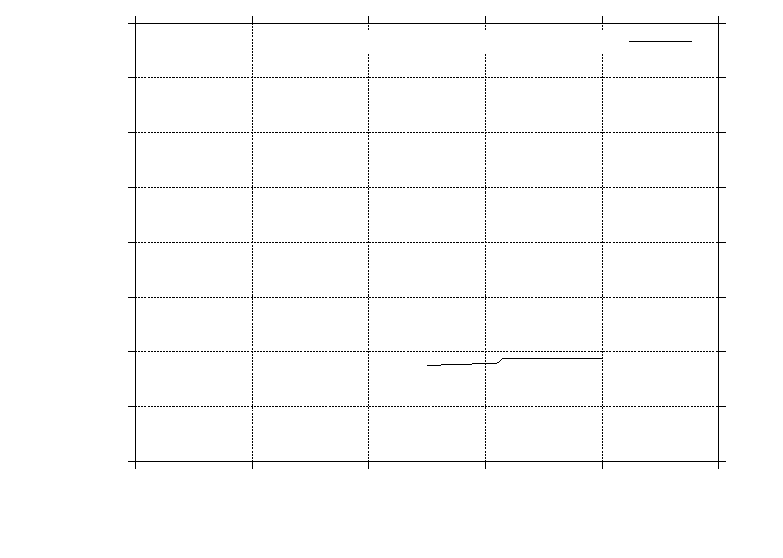
\includegraphics{E0ddepend}}%
    \gplfronttext
  \end{picture}%
\endgroup
  
\caption{The ground state free energy for $T = 0$, $E_0 + 2\mu N_F$, is plotted as a function of the interwire distance $d$. Black dashed: intrawire pairing only. Black dash-dotted: interwire pairing only. In red: $\Delta^{12}_k$ imaginary. In blue: $\Delta^{12}_k$ real. For the free gas: $(E_0 + 2\mu N_F)/\epsilon_{F,0}N_F = 2/3 = 0.667$. Parameters: $(n_Ba_B^3)^{1/3} = 0.01$, $(n_Ba_{BF}^3)^{1/3} = 0.11$, $l_t = 0$, $\frac{m_B}{m_F} = 7/40$, $\frac{n_F}{n_B^{1/3}} = 0.215$, $v_F/c_0 = 0.33$. }  
\label{fig.2wiresE0ddepend}  
\end{center}
\end{figure}

\begin{figure} 
\begin{center}  
% GNUPLOT: LaTeX picture with Postscript
\begingroup
  \makeatletter
  \providecommand\color[2][]{%
    \GenericError{(gnuplot) \space\space\space\@spaces}{%
      Package color not loaded in conjunction with
      terminal option `colourtext'%
    }{See the gnuplot documentation for explanation.%
    }{Either use 'blacktext' in gnuplot or load the package
      color.sty in LaTeX.}%
    \renewcommand\color[2][]{}%
  }%
  \providecommand\includegraphics[2][]{%
    \GenericError{(gnuplot) \space\space\space\@spaces}{%
      Package graphicx or graphics not loaded%
    }{See the gnuplot documentation for explanation.%
    }{The gnuplot epslatex terminal needs graphicx.sty or graphics.sty.}%
    \renewcommand\includegraphics[2][]{}%
  }%
  \providecommand\rotatebox[2]{#2}%
  \@ifundefined{ifGPcolor}{%
    \newif\ifGPcolor
    \GPcolorfalse
  }{}%
  \@ifundefined{ifGPblacktext}{%
    \newif\ifGPblacktext
    \GPblacktexttrue
  }{}%
  % define a \g@addto@macro without @ in the name:
  \let\gplgaddtomacro\g@addto@macro
  % define empty templates for all commands taking text:
  \gdef\gplbacktext{}%
  \gdef\gplfronttext{}%
  \makeatother
  \ifGPblacktext
    % no textcolor at all
    \def\colorrgb#1{}%
    \def\colorgray#1{}%
  \else
    % gray or color?
    \ifGPcolor
      \def\colorrgb#1{\color[rgb]{#1}}%
      \def\colorgray#1{\color[gray]{#1}}%
      \expandafter\def\csname LTw\endcsname{\color{white}}%
      \expandafter\def\csname LTb\endcsname{\color{black}}%
      \expandafter\def\csname LTa\endcsname{\color{black}}%
      \expandafter\def\csname LT0\endcsname{\color[rgb]{1,0,0}}%
      \expandafter\def\csname LT1\endcsname{\color[rgb]{0,1,0}}%
      \expandafter\def\csname LT2\endcsname{\color[rgb]{0,0,1}}%
      \expandafter\def\csname LT3\endcsname{\color[rgb]{1,0,1}}%
      \expandafter\def\csname LT4\endcsname{\color[rgb]{0,1,1}}%
      \expandafter\def\csname LT5\endcsname{\color[rgb]{1,1,0}}%
      \expandafter\def\csname LT6\endcsname{\color[rgb]{0,0,0}}%
      \expandafter\def\csname LT7\endcsname{\color[rgb]{1,0.3,0}}%
      \expandafter\def\csname LT8\endcsname{\color[rgb]{0.5,0.5,0.5}}%
    \else
      % gray
      \def\colorrgb#1{\color{black}}%
      \def\colorgray#1{\color[gray]{#1}}%
      \expandafter\def\csname LTw\endcsname{\color{white}}%
      \expandafter\def\csname LTb\endcsname{\color{black}}%
      \expandafter\def\csname LTa\endcsname{\color{black}}%
      \expandafter\def\csname LT0\endcsname{\color{black}}%
      \expandafter\def\csname LT1\endcsname{\color{black}}%
      \expandafter\def\csname LT2\endcsname{\color{black}}%
      \expandafter\def\csname LT3\endcsname{\color{black}}%
      \expandafter\def\csname LT4\endcsname{\color{black}}%
      \expandafter\def\csname LT5\endcsname{\color{black}}%
      \expandafter\def\csname LT6\endcsname{\color{black}}%
      \expandafter\def\csname LT7\endcsname{\color{black}}%
      \expandafter\def\csname LT8\endcsname{\color{black}}%
    \fi
  \fi
    \setlength{\unitlength}{0.0500bp}%
    \ifx\gptboxheight\undefined%
      \newlength{\gptboxheight}%
      \newlength{\gptboxwidth}%
      \newsavebox{\gptboxtext}%
    \fi%
    \setlength{\fboxrule}{0.5pt}%
    \setlength{\fboxsep}{1pt}%
\begin{picture}(7200.00,5040.00)%
    \gplgaddtomacro\gplbacktext{%
      \csname LTb\endcsname%
      \put(814,767){\makebox(0,0)[r]{\strut{}$0$}}%
      \csname LTb\endcsname%
      \put(814,1469){\makebox(0,0)[r]{\strut{}$0.1$}}%
      \csname LTb\endcsname%
      \put(814,2170){\makebox(0,0)[r]{\strut{}$0.2$}}%
      \csname LTb\endcsname%
      \put(814,2872){\makebox(0,0)[r]{\strut{}$0.3$}}%
      \csname LTb\endcsname%
      \put(814,3573){\makebox(0,0)[r]{\strut{}$0.4$}}%
      \csname LTb\endcsname%
      \put(814,4275){\makebox(0,0)[r]{\strut{}$0.5$}}%
      \csname LTb\endcsname%
      \put(814,4976){\makebox(0,0)[r]{\strut{}$0.6$}}%
      \csname LTb\endcsname%
      \put(1009,484){\makebox(0,0){\strut{}$0.71$}}%
      \csname LTb\endcsname%
      \put(1828,484){\makebox(0,0){\strut{}$0.72$}}%
      \csname LTb\endcsname%
      \put(2646,484){\makebox(0,0){\strut{}$0.73$}}%
      \csname LTb\endcsname%
      \put(3465,484){\makebox(0,0){\strut{}$0.74$}}%
      \csname LTb\endcsname%
      \put(4284,484){\makebox(0,0){\strut{}$0.75$}}%
      \csname LTb\endcsname%
      \put(5103,484){\makebox(0,0){\strut{}$0.76$}}%
      \csname LTb\endcsname%
      \put(5921,484){\makebox(0,0){\strut{}$0.77$}}%
      \csname LTb\endcsname%
      \put(6740,484){\makebox(0,0){\strut{}$0.78$}}%
    }%
    \gplgaddtomacro\gplfronttext{%
      \csname LTb\endcsname%
      \put(176,2871){\rotatebox{-270}{\makebox(0,0){\strut{}$Delta_k/epsilon_{F,0}$}}}%
      \put(3874,154){\makebox(0,0){\strut{}$k_Fd$}}%
      \csname LTb\endcsname%
      \put(3385,4803){\makebox(0,0)[r]{\strut{}$Intrawire pairing$}}%
      \csname LTb\endcsname%
      \put(3385,4583){\makebox(0,0)[r]{\strut{}$Interwire pairing$}}%
    }%
    \gplbacktext
    \put(0,0){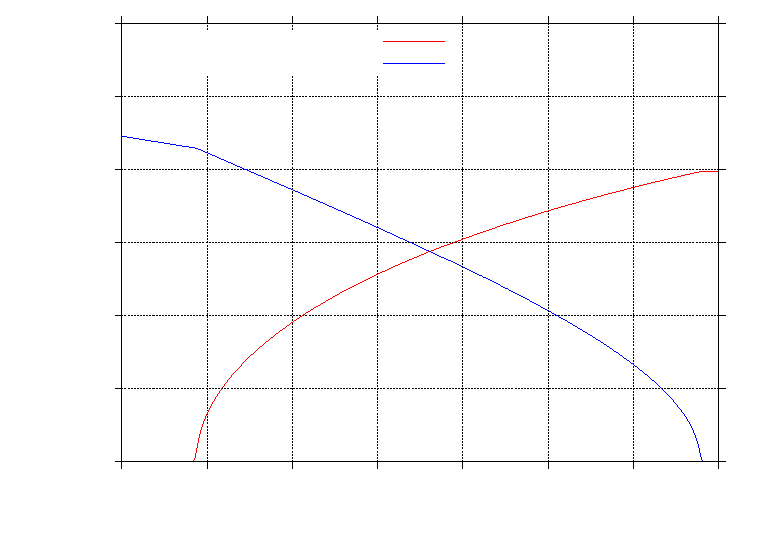
\includegraphics{ddepend}}%
    \gplfronttext
  \end{picture}%
\endgroup
  
\caption{The maximal pairings $\max_k\left[\left|\Delta^{11}_k\right|\right]$ and $\max_k\left[\left|\Delta^{12}_k\right|\right]$ as a function of the distance $d$ between the wires. In red: pairings for $\Delta^{12}_k$ imaginary, corresponding to the red graph in figure \ref{fig.2wiresE0ddepend}. In blue: Pairings for $\Delta^{12}_k$ real, corresponding to the blue graph in figure \ref{fig.2wiresE0ddepend}. Parameters: $(n_Ba_B^3)^{1/3} = 0.01$, $(n_Ba_{BF}^3)^{1/3} = 0.11$, $l_t = 0$, $\frac{m_B}{m_F} = 7/40$, $\frac{n_F}{n_B^{1/3}} = 0.215$, $v_F/c_0 = 0.33$. }  
\label{fig.2wiresMaximalPairingddepend}  
\end{center}    
\end{figure}
 
We see, that for small and large distances the expected behaviour is observed. Naively it seems to be the case, that the interwire pairing increases linearly for small $k_Fd$. However, an analysis to lower values of $d$ shows, that it diverges for $d \to 0$ as expected. In between we see a continuous cross over region, where both pairings are present. Further, we notice that the intrawire pairing is constant from just under $k_Fd = 0.78$ and upwards as we expected. The fact that we start at $k_Fd = k_Fd_c = 0.748$, and then iterate downwards and upwards from there is the reason for the very small indent in the data precisely at this value.

The figure only shows the maximal pairing $\max_k[|\Delta_k|]$. The same analysis also gives us, how the pairings functionally change as the distance $d$ is varied. This is summarized in figure \ref{fig.pairingkdependT0dvaried}. This explicitly shows, that the interwire pairing is even in $k$ and hence is a $s$-wave type pairing. We see, that it has its maximum value at $k=0$ as one might expect from the interwire induced interaction. Further, it shows no oscillatory behaviour, it simply decays exponentially for large values of $k$. The intrawire pairing is seen to have the same functional form as for the single wire, hence a $p$-wave type pairing. The overall behaviour of the pairings are seen to be independent of $d$. The interwire pairing is simply enhanced as $d$ decreases, vice versa for the intrawire pairing.  

\begin{figure} 
\begin{center}  
% GNUPLOT: LaTeX picture with Postscript
\begingroup
  \makeatletter
  \providecommand\color[2][]{%
    \GenericError{(gnuplot) \space\space\space\@spaces}{%
      Package color not loaded in conjunction with
      terminal option `colourtext'%
    }{See the gnuplot documentation for explanation.%
    }{Either use 'blacktext' in gnuplot or load the package
      color.sty in LaTeX.}%
    \renewcommand\color[2][]{}%
  }%
  \providecommand\includegraphics[2][]{%
    \GenericError{(gnuplot) \space\space\space\@spaces}{%
      Package graphicx or graphics not loaded%
    }{See the gnuplot documentation for explanation.%
    }{The gnuplot epslatex terminal needs graphicx.sty or graphics.sty.}%
    \renewcommand\includegraphics[2][]{}%
  }%
  \providecommand\rotatebox[2]{#2}%
  \@ifundefined{ifGPcolor}{%
    \newif\ifGPcolor
    \GPcolorfalse
  }{}%
  \@ifundefined{ifGPblacktext}{%
    \newif\ifGPblacktext
    \GPblacktexttrue
  }{}%
  % define a \g@addto@macro without @ in the name:
  \let\gplgaddtomacro\g@addto@macro
  % define empty templates for all commands taking text:
  \gdef\gplbacktext{}%
  \gdef\gplfronttext{}%
  \makeatother
  \ifGPblacktext
    % no textcolor at all
    \def\colorrgb#1{}%
    \def\colorgray#1{}%
  \else
    % gray or color?
    \ifGPcolor
      \def\colorrgb#1{\color[rgb]{#1}}%
      \def\colorgray#1{\color[gray]{#1}}%
      \expandafter\def\csname LTw\endcsname{\color{white}}%
      \expandafter\def\csname LTb\endcsname{\color{black}}%
      \expandafter\def\csname LTa\endcsname{\color{black}}%
      \expandafter\def\csname LT0\endcsname{\color[rgb]{1,0,0}}%
      \expandafter\def\csname LT1\endcsname{\color[rgb]{0,1,0}}%
      \expandafter\def\csname LT2\endcsname{\color[rgb]{0,0,1}}%
      \expandafter\def\csname LT3\endcsname{\color[rgb]{1,0,1}}%
      \expandafter\def\csname LT4\endcsname{\color[rgb]{0,1,1}}%
      \expandafter\def\csname LT5\endcsname{\color[rgb]{1,1,0}}%
      \expandafter\def\csname LT6\endcsname{\color[rgb]{0,0,0}}%
      \expandafter\def\csname LT7\endcsname{\color[rgb]{1,0.3,0}}%
      \expandafter\def\csname LT8\endcsname{\color[rgb]{0.5,0.5,0.5}}%
    \else
      % gray
      \def\colorrgb#1{\color{black}}%
      \def\colorgray#1{\color[gray]{#1}}%
      \expandafter\def\csname LTw\endcsname{\color{white}}%
      \expandafter\def\csname LTb\endcsname{\color{black}}%
      \expandafter\def\csname LTa\endcsname{\color{black}}%
      \expandafter\def\csname LT0\endcsname{\color{black}}%
      \expandafter\def\csname LT1\endcsname{\color{black}}%
      \expandafter\def\csname LT2\endcsname{\color{black}}%
      \expandafter\def\csname LT3\endcsname{\color{black}}%
      \expandafter\def\csname LT4\endcsname{\color{black}}%
      \expandafter\def\csname LT5\endcsname{\color{black}}%
      \expandafter\def\csname LT6\endcsname{\color{black}}%
      \expandafter\def\csname LT7\endcsname{\color{black}}%
      \expandafter\def\csname LT8\endcsname{\color{black}}%
    \fi
  \fi
    \setlength{\unitlength}{0.0500bp}%
    \ifx\gptboxheight\undefined%
      \newlength{\gptboxheight}%
      \newlength{\gptboxwidth}%
      \newsavebox{\gptboxtext}%
    \fi%
    \setlength{\fboxrule}{0.5pt}%
    \setlength{\fboxsep}{1pt}%
\begin{picture}(7200.00,5040.00)%
    \gplgaddtomacro\gplbacktext{%
      \csname LTb\endcsname%
      \put(946,767){\makebox(0,0)[r]{\strut{}$-0.6$}}%
      \csname LTb\endcsname%
      \put(946,1468){\makebox(0,0)[r]{\strut{}$-0.4$}}%
      \csname LTb\endcsname%
      \put(946,2170){\makebox(0,0)[r]{\strut{}$-0.2$}}%
      \csname LTb\endcsname%
      \put(946,2871){\makebox(0,0)[r]{\strut{}$0$}}%
      \csname LTb\endcsname%
      \put(946,3573){\makebox(0,0)[r]{\strut{}$0.2$}}%
      \csname LTb\endcsname%
      \put(946,4275){\makebox(0,0)[r]{\strut{}$0.4$}}%
      \csname LTb\endcsname%
      \put(946,4976){\makebox(0,0)[r]{\strut{}$0.6$}}%
      \csname LTb\endcsname%
      \put(1141,484){\makebox(0,0){\strut{}$-10$}}%
      \csname LTb\endcsname%
      \put(2541,484){\makebox(0,0){\strut{}$-5$}}%
      \csname LTb\endcsname%
      \put(3941,484){\makebox(0,0){\strut{}$0$}}%
      \csname LTb\endcsname%
      \put(5340,484){\makebox(0,0){\strut{}$5$}}%
      \csname LTb\endcsname%
      \put(6740,484){\makebox(0,0){\strut{}$10$}}%
    }%
    \gplgaddtomacro\gplfronttext{%
      \csname LTb\endcsname%
      \put(176,2871){\rotatebox{-270}{\makebox(0,0){\strut{}$\Delta_k/\epsilon_{F,0}$}}}%
      \put(3940,154){\makebox(0,0){\strut{}$k/k_F$}}%
      \csname LTb\endcsname%
      \put(5753,1820){\makebox(0,0)[r]{\strut{}$k_Fd = 0.575$}}%
      \csname LTb\endcsname%
      \put(5753,1600){\makebox(0,0)[r]{\strut{}$k_Fd = 0.585$}}%
      \csname LTb\endcsname%
      \put(5753,1380){\makebox(0,0)[r]{\strut{}$k_Fd = 0.595$}}%
      \csname LTb\endcsname%
      \put(5753,1160){\makebox(0,0)[r]{\strut{}$k_Fd = 0.610$}}%
      \csname LTb\endcsname%
      \put(5753,940){\makebox(0,0)[r]{\strut{}$k_Fd = 0.620$}}%
    }%
    \gplbacktext
    \put(0,0){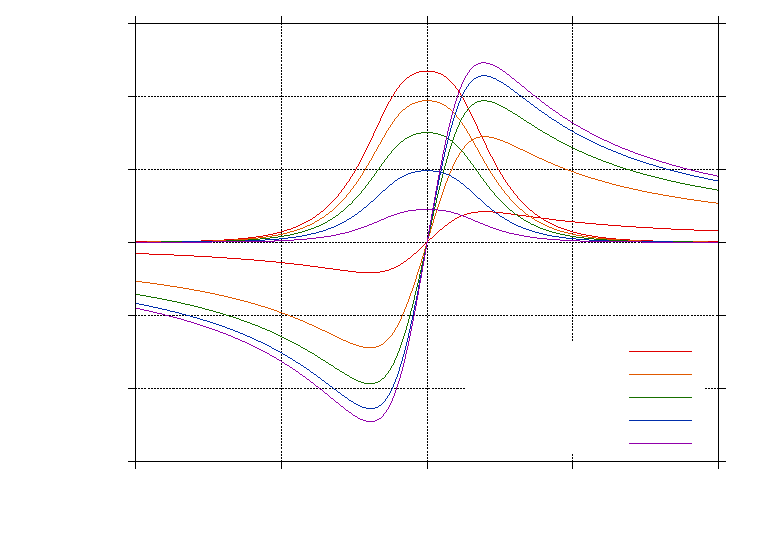
\includegraphics{Figures/twowires/Deltas1/kdepend}}%
    \gplfronttext
  \end{picture}%
\endgroup
  
\caption{The pairings $\Delta^{11}_k$ (odd) and $\Delta^{12}_k$ (even) plotted as a function of $k$. We see, that the functional behaviour is independent of $d$, and that there is a cross over between interwire and intrawire dominated pairing. The intrawire pairing is increased as $d$ increases. Vice versa for the interwire pairing. Parameters: $(n_Ba_B^3)^{1/3} = 0.01$, $(n_Ba_{BF}^3)^{1/3} = 0.11$, $l_t = 0$, $\frac{m_B}{m_F} = 7/40$, $\frac{n_F}{n_B^{1/3}} = 0.215$, $v_F/c_0 = 0.33$. }  
\label{fig.pairingkdependT0dvaried}  
\end{center}    
\end{figure}

The combined result of the three figures tells us the following. We are able to find a cross over region of interwire distances $d$, where both an interwire $s$-wave pairing and an intrawire $p$-wave pairing is present, and this transition is the energetically favourable. 

\section{Edge states and the curious cross over}
In this section we analyse the results of the previous section from a symmetry point of view. The analysis is based on the exact same ideas as in section \ref{sec.topindexandphases}. 

As pointed out in section \ref{sec.topindexandphases} the particle-hole symmetry ensures, that for every positive energy solution, there is also a negative one. For the separated wires sketched in the top of \ref{fig.2wiresedgestates} this has the same conclusion as in that section: there has to be a\textit{single} zero energy edge state which is robust against symmetry-conserving perturbations. The difference now is, that there is \textit{two} edge states: one for each wire. This has profound consequences. As we bring the wires closer together the system is perturbed by the interwire pairing $\Delta^{12}_k$. As shown in section \ref{sec.2wiressymmetries} this perturbation respects the particle-hole symmetry. This is simply because we are still dealing with a Bogoliubov de-Gennes system. 

\begin{figure}
\center
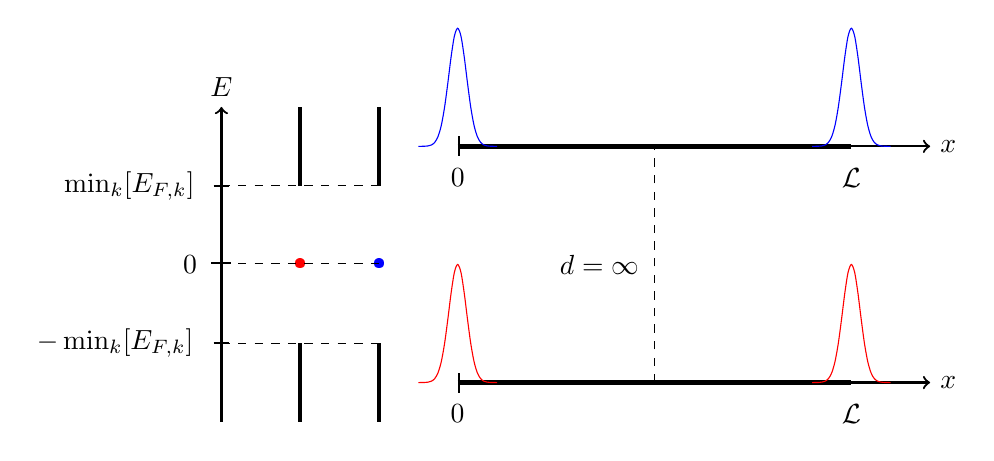
\begin{tikzpicture}
\draw[|->, thick] (0, 0) -- (0,  2) node[above]{$E$};
\draw[-, thick]   (0, 0) -- (0, -2);
\node at (-0.4, 0) {$0$};

\draw[-, dashed] (0, 1)--(2, 1);
\draw[-, thick] (-0.1, 1)--(0.1, 1);
\node at (-1.17,1) {$\min_k[E_{F,k}]$};

\draw[-, dashed] (0,    -1) -- (2,   -1);
\draw[-, thick]  (-0.1, -1) -- (0.1, -1);
\node at (-1.35,-1) {$-\min_k[E_{F,k}]$};

\draw[-, ultra thick] (1, 1)--(1, 2);
\draw[-, ultra thick] (1, -1)--(1, -2);
\node[red] at (1, 0) {\textbullet};

\draw[-, ultra thick] (2, 1)--(2, 2);
\draw[-, ultra thick] (2, -1)--(2, -2);
\node[blue] at (2, 0) {\textbullet};

\draw[-, dashed] (0,0.01) --(2,0.01);

\node at (3, -1.9) {$0$};
\node at (8, -1.9) {$\mathcal{L}$};
\draw[|->, thick ] (3,-1.5) -- (9,-1.5) node[right]{$x$};

\draw[-, ultra thick ] (3,-1.5) -- (8,-1.5);
\draw[scale=0.5,domain=-1:1,smooth,variable=\x,red] plot ({\x + 6},{ 3 * exp{- 10 * \x*\x} - 3});
\draw[scale=0.5,domain=-1:1,smooth,variable=\x,red] plot ({\x + 16},{ 3 * exp{- 10 * \x*\x} -3});

\node at (3, 1.1) {$0$};
\node at (8, 1.1) {$\mathcal{L}$};
\draw[|->, thick ] (3,1.5) -- (9,1.5) node[right]{$x$};

\draw[-, ultra thick] (3,1.5) -- (8,1.5);
\draw[scale=0.5,domain=-1:1,smooth,variable=\x,blue] plot ({\x + 6},{ 3 * exp{- 10 * \x*\x} + 3});
\draw[scale=0.5,domain=-1:1,smooth,variable=\x,blue] plot ({\x + 16},{ 3 * exp{- 10 * \x*\x} + 3});

\draw[-, dashed] (5.5, -1.5) -- (5.5, 1.5);
\node at (4.8, 0) {$d=\infty$};
\end{tikzpicture}

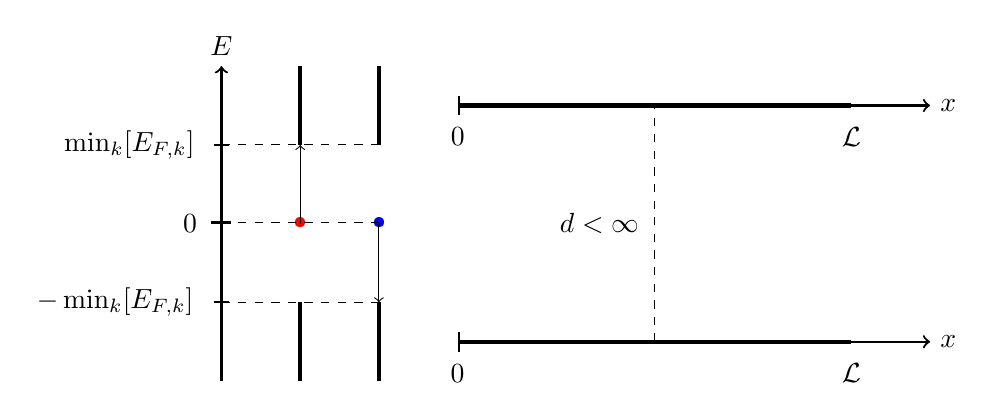
\begin{tikzpicture}
\draw[|->, thick] (0, 0) -- (0,  2) node[above]{$E$};
\draw[-, thick]   (0, 0) -- (0, -2);
\node at (-0.4, 0) {$0$};

\draw[-, dashed] (0, 1)--(2, 1);
\draw[-, thick] (-0.1, 1)--(0.1, 1);
\node at (-1.17,1) {$\min_k[E_{F,k}]$};

\draw[-, dashed] (0,    -1) -- (2,   -1);
\draw[-, thick]  (-0.1, -1) -- (0.1, -1);
\node at (-1.35,-1) {$-\min_k[E_{F,k}]$};

\draw[-, ultra thick] (1, 1)--(1, 2);
\draw[-, ultra thick] (1, -1)--(1, -2);
\node[red] at (1, 0) {\textbullet};
\draw[->] (1, 0) --  (1,  1);

\draw[-, ultra thick] (2, 1)--(2, 2);
\draw[-, ultra thick] (2, -1)--(2, -2);
\node[blue] at (2, 0) {\textbullet};
\draw[->] (2, 0) --  (2,  -1);

\draw[-, dashed] (0,0.01) --(2,0.01);

\node at (3, -1.9) {$0$};
\node at (8, -1.9) {$\mathcal{L}$};
\draw[|->, thick ] (3,-1.5) -- (9,-1.5) node[right]{$x$};

\draw[-, ultra thick ] (3,-1.5) -- (8,-1.5);

\node at (3, 1.1) {$0$};
\node at (8, 1.1) {$\mathcal{L}$};
\draw[|->, thick ] (3,1.5) -- (9,1.5) node[right]{$x$};

\draw[-, ultra thick] (3,1.5) -- (8,1.5);

\draw[-, dashed] (5.5, -1.5) -- (5.5, 1.5);
\node at (4.8, 0) {$d<\infty$};
\end{tikzpicture}
\caption{Top: for $d=\infty$ we have two copies of the single wire system. There are two symmetry-protected edge states, one at each wire. This is indicated with red and blue. Bottom: the interwire pairing respects the particle hole symmetry, but the edge states are no longer protected, since there are two of them. Consequently, there are no edge states.}
\label{fig.2wiresedgestates}
\end{figure}

Let us now first focus on the energetically favourable solution found in the previous section: $\Delta^{22}_k = - \Delta^{11}_k$ real and $\Delta^{12}_k$ imaginary. As shown in section \ref{sec.2wiressymmetries} this system has an additional time reversal symmetry that exhanges the wires, and that squares to $+\mathbb{I}$. However, there is nothing to protect the two edge states in the two wires from coupling, and since it is only the total spectrum that has to exhibit the plus/minus symmetry in the energies, the edge state energies can \textit{gap} away. This is sketched in the bottom of figure \ref{fig.2wiresedgestates}. This is exactly, what the numerical analysis says must be happening. The reason is the following. The separated wires exhibit only $p$-wave pairing, which has a topological ground state as shown in chapter \ref{Chapter7}. The closely spaced wires on the other hand have only $s$-wave pairing; a system that is known to be topologically trivial INDSÆT REFERENCE. Hence, according to the arguments of section \ref{sec.topindexandphases} either the bulk energy gap has to close, or the edge states are simply coupled and gapped away. In the case of an imaginary interwire pairing the energy dispersion is: $E_{F,k} = \sqrt{\varepsilon^2_k + (\Delta^{11}_k)^2 + |\Delta^{12}_k|^2 }$. This means, that the bulk energy gap \textit{cannot} close, since it only contains positive terms. The only possibility is that $\varepsilon_k, \Delta^{11}_k$ and $\Delta^{12}_k$ is zero at the same time. This is ruled out by the numerical analysis in figure \ref{fig.pairingkdependT0dvaried}. Since the bulk gap cannot close, the edge states are gapped.

The situation changes dramatically for the real interwire pairing case. As shown in section \ref{sec.2wiressymmetries} this means, that the system has a time reversal symmetry, that squares to $-\mathbb{I}$. The edge states are hereby protected by Kramers degeneracy. The argument closely follows the argument in \cite{Sakurai}. The time reversal symmetry is described by $\mathcal{T} = i\sigma_2 K$ in first quantization: $\mathcal{T}\mathcal{H}_{FF,k} = \mathcal{H}_{FF,-k}\mathcal{T}$. Let us now assume, that we have one state, $\ket{\psi_k}$, with energy $E_k$. Then $\mathcal{T}\ket{\psi_k}$ also has the energy $E_k$:
\begin{equation}
\mathcal{H}_{FF,-k}\mathcal{T}\ket{\psi_k} = \mathcal{T}\mathcal{H}_{FF,k}\ket{\psi_k} = E_k\mathcal{T}\ket{\psi_k}. \nonumber
\end{equation}
Let us suppose, that the two kets represent the same state. Then they are equal up to some phase: $\mathcal{T}\ket{\psi_k} = \text{e}^{i\delta}\ket{\psi_k}$. Further:
\begin{equation}
\mathcal{T}^2\ket{\psi_k} = \mathcal{T}\left(\text{e}^{i\delta}\ket{\psi_k}\right) = \text{e}^{-i\delta}\text{e}^{i\delta}\ket{\psi_k} = \ket{\psi_k}. \nonumber
\end{equation}
However, this contradicts that $\mathcal{T}^2 = -1$. Hence, the two kets must really represent two different states. This means, that any energy is at least doubly degenerate. This is Kramers degeneracy. Notice, that it is crucial that $\mathcal{T}^2 = -1$. For $\mathcal{T}^2 = +1$ there is no Kramers degeneracy. 

The question now is, how this changes the behaviour from the imaginary interwire pairing case, if we only look at perturbations, that respect all the symmetries of the system. Before the edge states could gap away: one to positive and one to negative energies. However, that is not possible here, because it would lead to only a single state at those two energies. Hence, the edge states are once again protected at $E = 0$. Since we now know, that we have to come from a topological to a trivial state something dramatic must happen in the cross over. In the same way as in section \ref{sec.topindexandphases} the switch in topological to trivial phase is associated with a closing in the bulk energy gap. The numerical analysis shows, that this happens at a single point $d = d_c$. The curious issue is, that if we look at the dispersion relations nothing stops this transition from being continuous as well:
\begin{equation}
E^{\pm}_{F,k} = \sqrt{\varepsilon^2_k + (\Delta^{11}_k)^2 + (\Delta^{12}_k)^2 \pm 2\Delta^{11}_k\Delta^{12}_k} = \sqrt{\varepsilon^2_k + (\Delta^{11}_k \pm \Delta^{12}_k)^2}. \nonumber
\end{equation}
From this it is clear, that if we had both pairings nonzero over an interval of $d$, then for some distance $d$, we would have $\Delta^{11}_{\pm k} = \mp \Delta^{12}_k$ at the Fermi surface, where $\varepsilon_k = \frac{k^2}{2m_F} - \mu =  0$, hence leading to $E^{\pm}_{F,\pm k} = 0$. However, this does not happen. The transition is abrupt at a single point, $d = d_c$. This numerical result is therefore not understood at the present stage. 

\section{Range of interaction dependency of cross over}
In this section we will investigate how the cross over from intrawire to interwire pairing depends on the range of the induced interaction. The range is roughly the condensate coherence length $\xi$:
\begin{equation}
k_F\frac{\xi}{\sqrt{2}} = \frac{\sqrt{\pi}}{4}\frac{1}{\sqrt{(n_Ba_B^3)^{1/3}}}\frac{n_F}{n_B^{1/3}}.
\label{eq.RangefunctionofrBBnB}
\end{equation}
It is intuitively reasonable, that for a longer interaction range, the interwire interaction will become comparable to the intrawire interaction at a larger critical distance $d_c$ between the wires. This is simply because the distance between the wires should become less significant for a longer interaction range. Hence, we expect a monotonic increase of $d_c$ with $\xi$.   

For the analysis, we will keep the Bose gas parameter $(n_Ba_B^3)^{1/3}$ constant and use the ratio of interparticle distances $n_F/n_B^{1/3}$ to vary the range of the interaction. The analysis is then performed in the following way. We start at a high value of $n_F/n_B^{1/3}$. A direct and precise measure for the transition is the previously mentioned critical distance $d_c$. In practice this is found in the following way. First we calculate the free energy $F_1(\Delta^{11}_k) = E_0(\Delta^{11}_k) + 2 \mu (\Delta^{11}_k) N_F$ in the case, that there is only intrawire pairing, $\Delta^{11}_k$ present. This is independent of $d$ as described by the dashed curve in figure \ref{fig.2wiresE0ddepend}. Then we calculate the same in the case, there is only interwire pairing, $\Delta^{12}_k$, present. We then iteratively find the value of $d = d_c$, where the free energies match: $F(\Delta^{12}_k, d_c) = F(\Delta^{11}_k)$. We then decrease $n_F/n_B^{1/3}$ by a small amount and repeat the process. The outcome of the analysis is shown in figure \ref{fig.twowirescrossovernBdepend}. We notice, that the $d_c$ exhibits a maximal value, and that it approaches a constant for large ratios of $n_F/n_B^{1/3}$. The red line indicates where $v_F = c_0$. Therefore, the behaviour to the right of the red line can only be considered as the zero frequency contribution. Hence, strictly we can only describe the effect of the zero frequency component. 

We can understand the appearance of the asymptotic behaviour from a functional point of view. The intrawire pairing, $\Delta^{11}_k$, depends on the parameters $\beta, m_B/m_F, (n_Ba_B^3)^{1/3}$ and $n_B^{1/3}/n_F$ and is a functional of the pairings themselves: $\Delta^{11}_k, \Delta^{12}_k$. This is similarly the case for the interwire pairing, $\Delta^{12}_k$, with the additional parameter $d$. Hence, we can write:
\begin{equation}
\Delta^{11}_k = F\left(\Delta^{11}_k, \Delta^{12}_k, \beta, \frac{m_B}{m_F}, (n_Ba_B^3)^{1/3}, \frac{n_B^{1/3}}{n_F} \right), \hspace{0.5cm} \Delta^{12}_k = G\left(\Delta^{11}_k, \Delta^{12}_k, \beta, \frac{m_B}{m_F}, (n_Ba_B^3)^{1/3}, \frac{n_B^{1/3}}{n_F}, d \right), \nonumber 
\end{equation}
where $F$ and $G$ are the described functionals. On unitless form the functionals have a common prefactor, that depends on the mass ratio, the Bose gas parameter and the ratio of interparticle distances: $m_B/m_F, (n_Ba_B^3)^{1/3}$, and $n_B^{1/3}/n_F$. This means, that the limit of $n_F/n_B^{1/3} \to \infty $ is well-defined for the ratio of the pairings:
\begin{equation}
\lim_{\frac{n_F}{n_B^{1/3}} \to \infty} \left[\frac{\max_k[|\Delta^{11}_k|]}{\max_k[|\Delta^{12}_k|]}\right] = \frac{\max_k\left[\left|F\left(\Delta^{11}_k, \Delta^{12}_k, \beta, \frac{m_B}{m_F}, (n_Ba_B^3)^{1/3}, \frac{n_B^{1/3}}{n_F} = 0 \right)\right|\right] }{\max_k\left[\left|G\left(\Delta^{11}_k, \Delta^{12}_k, \beta, \frac{m_B}{m_F}, (n_Ba_B^3)^{1/3}, \frac{n_B^{1/3}}{n_F} = 0, d \right)\right|\right]}. \nonumber
\end{equation}
Since the pairings must be comparable at a distance similar to $d_c$, the above ratio will be equal to 1 at a distance similar to $d_c$. It is therefore evident that $d_c$ is independent of the ratio of interparticle distances for $n_F/n_B^{1/3} \gg 1$. Hence, $d_c$ must approach a constant for increasing values of $n_F/n_B^{1/3}$. From equation \eqref{eq.RangefunctionofrBBnB} it is clear, that an increase in $n_F/n_B^{1/3}$ for a fixed Bose gas parameter $(n_Ba_B^3)^{1/3}$ gives an increase in the coherence length $k_F\xi$ and hence in the range of the interactions. Therefore, the behaviour described in this section is \textit{not} in agreement with the intuitive idea given in the end of chapter \ref{Chapter8}, that the interwire interaction will become significant at a distance around the range of the interaction!

\begin{figure} 
\begin{center}  
% GNUPLOT: LaTeX picture with Postscript
\begingroup
  \makeatletter
  \providecommand\color[2][]{%
    \GenericError{(gnuplot) \space\space\space\@spaces}{%
      Package color not loaded in conjunction with
      terminal option `colourtext'%
    }{See the gnuplot documentation for explanation.%
    }{Either use 'blacktext' in gnuplot or load the package
      color.sty in LaTeX.}%
    \renewcommand\color[2][]{}%
  }%
  \providecommand\includegraphics[2][]{%
    \GenericError{(gnuplot) \space\space\space\@spaces}{%
      Package graphicx or graphics not loaded%
    }{See the gnuplot documentation for explanation.%
    }{The gnuplot epslatex terminal needs graphicx.sty or graphics.sty.}%
    \renewcommand\includegraphics[2][]{}%
  }%
  \providecommand\rotatebox[2]{#2}%
  \@ifundefined{ifGPcolor}{%
    \newif\ifGPcolor
    \GPcolorfalse
  }{}%
  \@ifundefined{ifGPblacktext}{%
    \newif\ifGPblacktext
    \GPblacktexttrue
  }{}%
  % define a \g@addto@macro without @ in the name:
  \let\gplgaddtomacro\g@addto@macro
  % define empty templates for all commands taking text:
  \gdef\gplbacktext{}%
  \gdef\gplfronttext{}%
  \makeatother
  \ifGPblacktext
    % no textcolor at all
    \def\colorrgb#1{}%
    \def\colorgray#1{}%
  \else
    % gray or color?
    \ifGPcolor
      \def\colorrgb#1{\color[rgb]{#1}}%
      \def\colorgray#1{\color[gray]{#1}}%
      \expandafter\def\csname LTw\endcsname{\color{white}}%
      \expandafter\def\csname LTb\endcsname{\color{black}}%
      \expandafter\def\csname LTa\endcsname{\color{black}}%
      \expandafter\def\csname LT0\endcsname{\color[rgb]{1,0,0}}%
      \expandafter\def\csname LT1\endcsname{\color[rgb]{0,1,0}}%
      \expandafter\def\csname LT2\endcsname{\color[rgb]{0,0,1}}%
      \expandafter\def\csname LT3\endcsname{\color[rgb]{1,0,1}}%
      \expandafter\def\csname LT4\endcsname{\color[rgb]{0,1,1}}%
      \expandafter\def\csname LT5\endcsname{\color[rgb]{1,1,0}}%
      \expandafter\def\csname LT6\endcsname{\color[rgb]{0,0,0}}%
      \expandafter\def\csname LT7\endcsname{\color[rgb]{1,0.3,0}}%
      \expandafter\def\csname LT8\endcsname{\color[rgb]{0.5,0.5,0.5}}%
    \else
      % gray
      \def\colorrgb#1{\color{black}}%
      \def\colorgray#1{\color[gray]{#1}}%
      \expandafter\def\csname LTw\endcsname{\color{white}}%
      \expandafter\def\csname LTb\endcsname{\color{black}}%
      \expandafter\def\csname LTa\endcsname{\color{black}}%
      \expandafter\def\csname LT0\endcsname{\color{black}}%
      \expandafter\def\csname LT1\endcsname{\color{black}}%
      \expandafter\def\csname LT2\endcsname{\color{black}}%
      \expandafter\def\csname LT3\endcsname{\color{black}}%
      \expandafter\def\csname LT4\endcsname{\color{black}}%
      \expandafter\def\csname LT5\endcsname{\color{black}}%
      \expandafter\def\csname LT6\endcsname{\color{black}}%
      \expandafter\def\csname LT7\endcsname{\color{black}}%
      \expandafter\def\csname LT8\endcsname{\color{black}}%
    \fi
  \fi
    \setlength{\unitlength}{0.0500bp}%
    \ifx\gptboxheight\undefined%
      \newlength{\gptboxheight}%
      \newlength{\gptboxwidth}%
      \newsavebox{\gptboxtext}%
    \fi%
    \setlength{\fboxrule}{0.5pt}%
    \setlength{\fboxsep}{1pt}%
\begin{picture}(7200.00,5040.00)%
    \gplgaddtomacro\gplbacktext{%
    }%
    \gplgaddtomacro\gplfronttext{%
      \csname LTb\endcsname%
      \put(176,2871){\rotatebox{-270}{\makebox(0,0){\strut{}$k_Fd_c$}}}%
      \put(3874,154){\makebox(0,0){\strut{}$n_F/n_B^{1/3}$}}%
      \csname LTb\endcsname%
      \put(814,767){\makebox(0,0)[r]{\strut{}$0$}}%
      \csname LTb\endcsname%
      \put(814,1469){\makebox(0,0)[r]{\strut{}$0.2$}}%
      \csname LTb\endcsname%
      \put(814,2170){\makebox(0,0)[r]{\strut{}$0.4$}}%
      \csname LTb\endcsname%
      \put(814,2872){\makebox(0,0)[r]{\strut{}$0.6$}}%
      \csname LTb\endcsname%
      \put(814,3573){\makebox(0,0)[r]{\strut{}$0.8$}}%
      \csname LTb\endcsname%
      \put(814,4275){\makebox(0,0)[r]{\strut{}$1$}}%
      \csname LTb\endcsname%
      \put(814,4976){\makebox(0,0)[r]{\strut{}$1.2$}}%
      \csname LTb\endcsname%
      \put(1009,484){\makebox(0,0){\strut{}$0$}}%
      \csname LTb\endcsname%
      \put(1773,484){\makebox(0,0){\strut{}$0.2$}}%
      \csname LTb\endcsname%
      \put(2537,484){\makebox(0,0){\strut{}$0.4$}}%
      \csname LTb\endcsname%
      \put(3301,484){\makebox(0,0){\strut{}$0.6$}}%
      \csname LTb\endcsname%
      \put(4066,484){\makebox(0,0){\strut{}$0.8$}}%
      \csname LTb\endcsname%
      \put(4830,484){\makebox(0,0){\strut{}$1$}}%
      \csname LTb\endcsname%
      \put(5594,484){\makebox(0,0){\strut{}$1.2$}}%
      \csname LTb\endcsname%
      \put(6358,484){\makebox(0,0){\strut{}$1.4$}}%
      \put(1850,3924){\makebox(0,0)[l]{\strut{}Intrawire pairing only}}%
      \put(4142,2521){\makebox(0,0)[l]{\strut{}Interwire pairing only}}%
    }%
    \gplbacktext
    \put(0,0){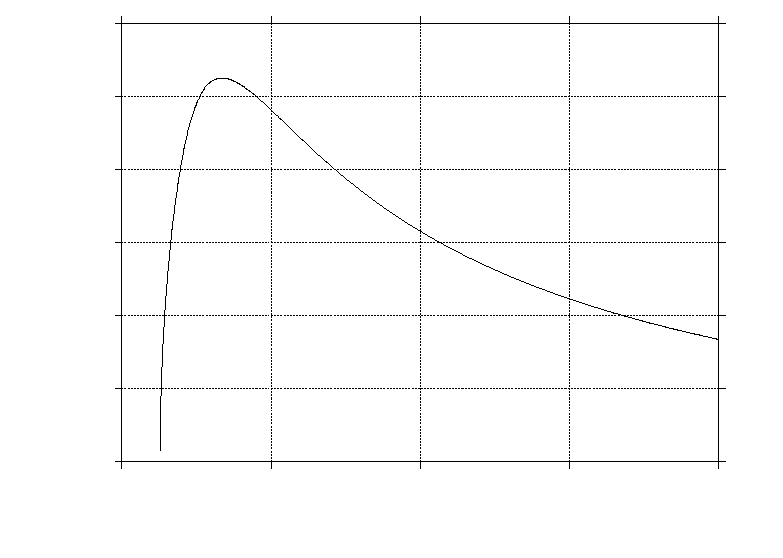
\includegraphics{Figures/twowires/Deltas3.1.3/nBdepend}}%
    \gplfronttext
  \end{picture}%
\endgroup
  
\caption{The critical distance $d_c$ plotted as a function of the ratio of interparticle distances $n_F/n_B^{1/3}$. Notice, that there is a maximum, at that $d_c$ approaches a constant for large $n_F/n_B^{1/3}$. The red line indicates, where $v_F = c_0$. The curve to the right hereof is only the zero frequency contribution. Parameters: $(n_Ba_B^3)^{1/3} = 0.01$, $(n_Ba_{BF}^3)^{1/3} = 0.11$, $l_t = 0$, $\frac{m_B}{m_F} = 7/40$. }  
\label{fig.twowirescrossovernBdepend}  
\end{center}    
\end{figure}

The appearance of a maximum in $d_c$ can qualitatively be understood in the following way. For low values of $n_F/n_B^{1/3}$ the Bose gas becomes more rigid, since the spacing between the bosons becomes smaller. Hence, the wires must be brought closer together for the interwire pairing to dominate. For high values of $n_F/n_B^{1/3}$ the Bose gas is depleted. This means, that there are simply fewer bosons for the fermions to interact with. It is therefore reasonable, that $d_c$ should not exhibit a maximal value for $n_F/n_B^{1/3} \to \infty$. As a consequence a maximal value of $d_c$ appeares. This analysis is reminiscent of the analysis explaning the appearance of a minimum in $W^\text{ind}_{FF,12}(k_F,k_F)$ as a function of $n_F/n_B^{1/3}$. See subsection \ref{subsec.relevantmomenta.effectiveinteraction} for the details.  

The result of this section is experimentally relevant. In a real experiment one might speculate in controlling the felt distance between the wires by tuning the coherence length. This may be an easier task, than physically moving the wires, since one here as to adjust the traps. However, the analysis in this section shows, that this cannot be done, at least not through putting more bosons into the gas. Why? - because one would then need the critical distance $d_c \to \infty$ for $n_F/n_B^{1/3} \to \infty$. In contradiction with the results of this section. The only possibility left is to adjust the Bose gas parameter $(n_Ba_B^3)^{1/3}$. 

SNAK MED GEORG OM DETTE.  

\section{Temperature dependency of pairings}
In this section we will investigate, how the pairings depend on temperature. The analysis is performed in complete analogy to the one in subsection \ref{subsec.momentum_and_temperature_pairing_singlewire}. 

For small and large distances, where one of the pairings is dominant, it is not difficult to imagine, what will happen. Here we expect, that the two pairings go to zero in a similar manner to single wire at two different critical temperatures. The dominant pairing for $T = 0$ will have the highest critical temperature. However, a couple questions arise. How does it affect the dominant pairing, that the suppressed pairing goes to zero? And is the interwire or intrawire pairing the more robust to a rise in temperature?

To answer these questions we investigate three cases, two where one pairing is strongly dominant, and one where the pairings are essentially equal for $T = 0$. The more interesting case is definitely the latter one, since this directly tests what pairing is the more robust. However, we might also gain some insight from the former. 

The result of the analysis for a dominant interwire pairing is shown in figure \ref{fig.maximalpairingsTdepend_2wires}. We see, that the overall expected behaviour is observed. We observe that the interwire pairing has a small kink, where the intrawire pairing vanishes. This emphasizes, that one pairing influences the functional behaviour of the other. Further, above this first critical temperature the maximal interwire pairing is astonishingly well described by the following relation:
\begin{equation}
\max_k[\Delta^{12}_k(T)] = \alpha \max_k[\Delta^{12}_k(T = 0)] \sqrt{1 - \left(\frac{T}{T_c}\right)^3}. 
\end{equation}
The coefficient $\alpha$ is close to $1$, but seems to depend slightly on the other parameters of the problem. For the present set of parameters we have $\alpha = 1.075$. This functional behaviour is the same as the single wire asymptotic form of the intrawire pairing apart from the $\alpha$ coefficient. Also, the agreement between the actual behaviour of the pairing and the asymptotic form kicks in earlier and to a higher degree in the present case. 

\begin{figure} 
\begin{center}  
% GNUPLOT: LaTeX picture with Postscript
\begingroup
  \makeatletter
  \providecommand\color[2][]{%
    \GenericError{(gnuplot) \space\space\space\@spaces}{%
      Package color not loaded in conjunction with
      terminal option `colourtext'%
    }{See the gnuplot documentation for explanation.%
    }{Either use 'blacktext' in gnuplot or load the package
      color.sty in LaTeX.}%
    \renewcommand\color[2][]{}%
  }%
  \providecommand\includegraphics[2][]{%
    \GenericError{(gnuplot) \space\space\space\@spaces}{%
      Package graphicx or graphics not loaded%
    }{See the gnuplot documentation for explanation.%
    }{The gnuplot epslatex terminal needs graphicx.sty or graphics.sty.}%
    \renewcommand\includegraphics[2][]{}%
  }%
  \providecommand\rotatebox[2]{#2}%
  \@ifundefined{ifGPcolor}{%
    \newif\ifGPcolor
    \GPcolorfalse
  }{}%
  \@ifundefined{ifGPblacktext}{%
    \newif\ifGPblacktext
    \GPblacktexttrue
  }{}%
  % define a \g@addto@macro without @ in the name:
  \let\gplgaddtomacro\g@addto@macro
  % define empty templates for all commands taking text:
  \gdef\gplbacktext{}%
  \gdef\gplfronttext{}%
  \makeatother
  \ifGPblacktext
    % no textcolor at all
    \def\colorrgb#1{}%
    \def\colorgray#1{}%
  \else
    % gray or color?
    \ifGPcolor
      \def\colorrgb#1{\color[rgb]{#1}}%
      \def\colorgray#1{\color[gray]{#1}}%
      \expandafter\def\csname LTw\endcsname{\color{white}}%
      \expandafter\def\csname LTb\endcsname{\color{black}}%
      \expandafter\def\csname LTa\endcsname{\color{black}}%
      \expandafter\def\csname LT0\endcsname{\color[rgb]{1,0,0}}%
      \expandafter\def\csname LT1\endcsname{\color[rgb]{0,1,0}}%
      \expandafter\def\csname LT2\endcsname{\color[rgb]{0,0,1}}%
      \expandafter\def\csname LT3\endcsname{\color[rgb]{1,0,1}}%
      \expandafter\def\csname LT4\endcsname{\color[rgb]{0,1,1}}%
      \expandafter\def\csname LT5\endcsname{\color[rgb]{1,1,0}}%
      \expandafter\def\csname LT6\endcsname{\color[rgb]{0,0,0}}%
      \expandafter\def\csname LT7\endcsname{\color[rgb]{1,0.3,0}}%
      \expandafter\def\csname LT8\endcsname{\color[rgb]{0.5,0.5,0.5}}%
    \else
      % gray
      \def\colorrgb#1{\color{black}}%
      \def\colorgray#1{\color[gray]{#1}}%
      \expandafter\def\csname LTw\endcsname{\color{white}}%
      \expandafter\def\csname LTb\endcsname{\color{black}}%
      \expandafter\def\csname LTa\endcsname{\color{black}}%
      \expandafter\def\csname LT0\endcsname{\color{black}}%
      \expandafter\def\csname LT1\endcsname{\color{black}}%
      \expandafter\def\csname LT2\endcsname{\color{black}}%
      \expandafter\def\csname LT3\endcsname{\color{black}}%
      \expandafter\def\csname LT4\endcsname{\color{black}}%
      \expandafter\def\csname LT5\endcsname{\color{black}}%
      \expandafter\def\csname LT6\endcsname{\color{black}}%
      \expandafter\def\csname LT7\endcsname{\color{black}}%
      \expandafter\def\csname LT8\endcsname{\color{black}}%
    \fi
  \fi
    \setlength{\unitlength}{0.0500bp}%
    \ifx\gptboxheight\undefined%
      \newlength{\gptboxheight}%
      \newlength{\gptboxwidth}%
      \newsavebox{\gptboxtext}%
    \fi%
    \setlength{\fboxrule}{0.5pt}%
    \setlength{\fboxsep}{1pt}%
\begin{picture}(7200.00,5040.00)%
    \gplgaddtomacro\gplbacktext{%
      \csname LTb\endcsname%
      \put(814,767){\makebox(0,0)[r]{\strut{}$0$}}%
      \csname LTb\endcsname%
      \put(814,1609){\makebox(0,0)[r]{\strut{}$0.1$}}%
      \csname LTb\endcsname%
      \put(814,2451){\makebox(0,0)[r]{\strut{}$0.2$}}%
      \csname LTb\endcsname%
      \put(814,3292){\makebox(0,0)[r]{\strut{}$0.3$}}%
      \csname LTb\endcsname%
      \put(814,4134){\makebox(0,0)[r]{\strut{}$0.4$}}%
      \csname LTb\endcsname%
      \put(814,4976){\makebox(0,0)[r]{\strut{}$0.5$}}%
      \csname LTb\endcsname%
      \put(1009,484){\makebox(0,0){\strut{}$0$}}%
      \csname LTb\endcsname%
      \put(1964,484){\makebox(0,0){\strut{}$0.05$}}%
      \csname LTb\endcsname%
      \put(2919,484){\makebox(0,0){\strut{}$0.1$}}%
      \csname LTb\endcsname%
      \put(3875,484){\makebox(0,0){\strut{}$0.15$}}%
      \csname LTb\endcsname%
      \put(4830,484){\makebox(0,0){\strut{}$0.2$}}%
      \csname LTb\endcsname%
      \put(5785,484){\makebox(0,0){\strut{}$0.25$}}%
      \csname LTb\endcsname%
      \put(6740,484){\makebox(0,0){\strut{}$0.3$}}%
    }%
    \gplgaddtomacro\gplfronttext{%
      \csname LTb\endcsname%
      \put(176,2871){\rotatebox{-270}{\makebox(0,0){\strut{}$\max_k[\Delta_k]/\epsilon_{F,0}$}}}%
      \put(3874,154){\makebox(0,0){\strut{}$T/T_F$}}%
    }%
    \gplbacktext
    \put(0,0){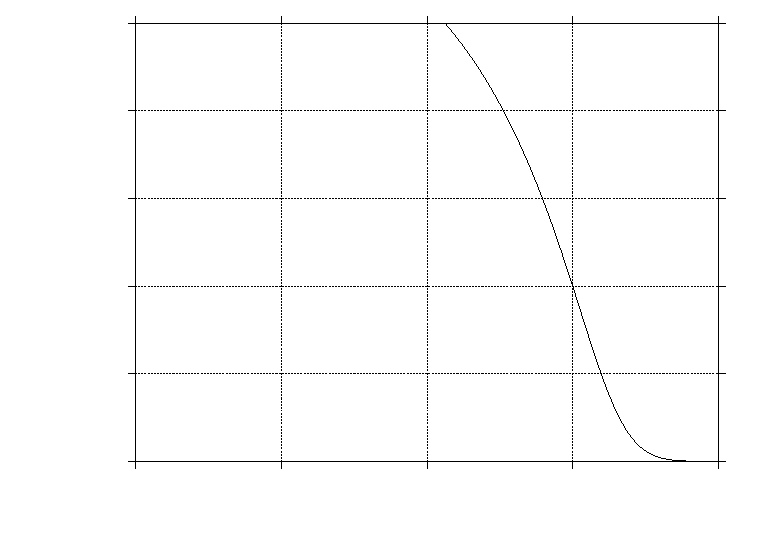
\includegraphics{Figures/twowires/Deltas4.5/Tdepend}}%
    \gplfronttext
  \end{picture}%
\endgroup
  
\caption{The maximal intrawire and interwire pairing $\max_k[|\Delta^{11}_k|]$ and $\max_k[|\Delta^{12}_k|]$ are plotted in black and magenta as a function of temperature. In blue and red the corresponding asymptotic forms from the single wire analysis, equation \eqref{eq.maxpairingasymp}. Notice, that there are two critical temperatures, and that the interwire pairing shows a kink, where the intrawire pairing goes to zero. Parameters: $k_Fd = 0.61$, $(n_Ba_B^3)^{1/3} = 0.01$, $(n_Ba_{BF}^3)^{1/3} = 0.11$, $l_t = 0$, $\frac{m_B}{m_F} = 7/40$, $\frac{n_F}{n_B^{1/3}} = 0.215$, $v_F/c_0 = 0.33$.}  
\label{fig.maximalpairingsTdepend_2wires}  
\end{center}    
\end{figure} 



 



% Chapter 11

\chapter{Continuous cross over: pairings and pair wave functions} % Main chapter title

\label{Chapter11} % For referencing the chapter elsewhere, use \ref{Chapter9} 

\lhead{Part III. \emph{Two wires}}
\chead{Chapter 11. \emph{Pairings \& pair wave functions}} % This is for the header on each page - perhaps a shortened title
%----------------------------------------------------------------------------------------
In this chapter we investigate the functional behaviour of the pairings and pair wave functions as a function of the interwire distance, $d$, in the case of the energetically favourable continuous cross over. This is done in section \ref{sec.2wirespairingspairwavefunction}. Further, in section \ref{sec.2wirespairingstemperature} we investigate the temperature dependence of the pairings. 

\section{Functional behaviour} \label{sec.2wirespairingspairwavefunction}
In this section we numerically calculate the functional behaviour of the pairings and the pair wave functions for the continuous cross over. The analysis is performed in the same manner as in section \ref{sec.2wiresCrossover_energy}. 

For the sake of clarity we again write up the gap equations in the case $\Delta^{22}_k = - \Delta^{11}_k$ real and $\Delta^{12}_k$ purely imaginary, which we found to support the continuous cross over:
\begin{align}
\Delta^{11}_k &= -\frac{1}{\mathcal{L}}\sum_{k'} W_{\text{ind}}^{11}(k, k')\frac{\Delta^{11}_{k'}}{2E_{F,k'}}\tanh\left(\frac{\beta E_{F,k'}}{2}\right), \nonumber \\
\Delta^{12}_k &= -\frac{1}{\mathcal{L}}\sum_{k'} W_{\text{ind}}^{12}(k, k')\frac{\Delta^{12}_{k'}}{2E_{F,k'}}\tanh\left(\frac{\beta E_{F,k'}}{2}\right), \nonumber
\end{align} 
with $E_{F,k} = \sqrt{\varepsilon^2_k + (\Delta^{11}_k)^2 + |\Delta^{12}_k|^2}$. We numerically find self-consistent solutions to the above gap equations along with the number equation \eqref{eq.2wiresnumberequation}. This is summarized in figure \ref{fig.pairingkdependT0dvaried}. It explicitly shows, that the interwire pairing is even in $k$ and hence is a $s$-wave type pairing. We see, that it has its maximum value at $k = 0$ as one might expect from the interwire induced interaction. Further, it shows no oscillatory behaviour, it simply decays exponentially for large values of $k$. The intrawire pairing is seen to have the same functional form as for the single wire, hence a $p$-wave type pairing. The overall behaviour of the pairings are seen to be independent of $d$. The interwire pairing is simply enhanced as $d$ decreases, vice versa for the intrawire pairing.  

\begin{figure} 
\begin{center}  
% GNUPLOT: LaTeX picture with Postscript
\begingroup
  \makeatletter
  \providecommand\color[2][]{%
    \GenericError{(gnuplot) \space\space\space\@spaces}{%
      Package color not loaded in conjunction with
      terminal option `colourtext'%
    }{See the gnuplot documentation for explanation.%
    }{Either use 'blacktext' in gnuplot or load the package
      color.sty in LaTeX.}%
    \renewcommand\color[2][]{}%
  }%
  \providecommand\includegraphics[2][]{%
    \GenericError{(gnuplot) \space\space\space\@spaces}{%
      Package graphicx or graphics not loaded%
    }{See the gnuplot documentation for explanation.%
    }{The gnuplot epslatex terminal needs graphicx.sty or graphics.sty.}%
    \renewcommand\includegraphics[2][]{}%
  }%
  \providecommand\rotatebox[2]{#2}%
  \@ifundefined{ifGPcolor}{%
    \newif\ifGPcolor
    \GPcolorfalse
  }{}%
  \@ifundefined{ifGPblacktext}{%
    \newif\ifGPblacktext
    \GPblacktexttrue
  }{}%
  % define a \g@addto@macro without @ in the name:
  \let\gplgaddtomacro\g@addto@macro
  % define empty templates for all commands taking text:
  \gdef\gplbacktext{}%
  \gdef\gplfronttext{}%
  \makeatother
  \ifGPblacktext
    % no textcolor at all
    \def\colorrgb#1{}%
    \def\colorgray#1{}%
  \else
    % gray or color?
    \ifGPcolor
      \def\colorrgb#1{\color[rgb]{#1}}%
      \def\colorgray#1{\color[gray]{#1}}%
      \expandafter\def\csname LTw\endcsname{\color{white}}%
      \expandafter\def\csname LTb\endcsname{\color{black}}%
      \expandafter\def\csname LTa\endcsname{\color{black}}%
      \expandafter\def\csname LT0\endcsname{\color[rgb]{1,0,0}}%
      \expandafter\def\csname LT1\endcsname{\color[rgb]{0,1,0}}%
      \expandafter\def\csname LT2\endcsname{\color[rgb]{0,0,1}}%
      \expandafter\def\csname LT3\endcsname{\color[rgb]{1,0,1}}%
      \expandafter\def\csname LT4\endcsname{\color[rgb]{0,1,1}}%
      \expandafter\def\csname LT5\endcsname{\color[rgb]{1,1,0}}%
      \expandafter\def\csname LT6\endcsname{\color[rgb]{0,0,0}}%
      \expandafter\def\csname LT7\endcsname{\color[rgb]{1,0.3,0}}%
      \expandafter\def\csname LT8\endcsname{\color[rgb]{0.5,0.5,0.5}}%
    \else
      % gray
      \def\colorrgb#1{\color{black}}%
      \def\colorgray#1{\color[gray]{#1}}%
      \expandafter\def\csname LTw\endcsname{\color{white}}%
      \expandafter\def\csname LTb\endcsname{\color{black}}%
      \expandafter\def\csname LTa\endcsname{\color{black}}%
      \expandafter\def\csname LT0\endcsname{\color{black}}%
      \expandafter\def\csname LT1\endcsname{\color{black}}%
      \expandafter\def\csname LT2\endcsname{\color{black}}%
      \expandafter\def\csname LT3\endcsname{\color{black}}%
      \expandafter\def\csname LT4\endcsname{\color{black}}%
      \expandafter\def\csname LT5\endcsname{\color{black}}%
      \expandafter\def\csname LT6\endcsname{\color{black}}%
      \expandafter\def\csname LT7\endcsname{\color{black}}%
      \expandafter\def\csname LT8\endcsname{\color{black}}%
    \fi
  \fi
    \setlength{\unitlength}{0.0500bp}%
    \ifx\gptboxheight\undefined%
      \newlength{\gptboxheight}%
      \newlength{\gptboxwidth}%
      \newsavebox{\gptboxtext}%
    \fi%
    \setlength{\fboxrule}{0.5pt}%
    \setlength{\fboxsep}{1pt}%
\begin{picture}(7200.00,5040.00)%
    \gplgaddtomacro\gplbacktext{%
      \csname LTb\endcsname%
      \put(946,767){\makebox(0,0)[r]{\strut{}$-0.6$}}%
      \csname LTb\endcsname%
      \put(946,1468){\makebox(0,0)[r]{\strut{}$-0.4$}}%
      \csname LTb\endcsname%
      \put(946,2170){\makebox(0,0)[r]{\strut{}$-0.2$}}%
      \csname LTb\endcsname%
      \put(946,2871){\makebox(0,0)[r]{\strut{}$0$}}%
      \csname LTb\endcsname%
      \put(946,3573){\makebox(0,0)[r]{\strut{}$0.2$}}%
      \csname LTb\endcsname%
      \put(946,4275){\makebox(0,0)[r]{\strut{}$0.4$}}%
      \csname LTb\endcsname%
      \put(946,4976){\makebox(0,0)[r]{\strut{}$0.6$}}%
      \csname LTb\endcsname%
      \put(1141,484){\makebox(0,0){\strut{}$-10$}}%
      \csname LTb\endcsname%
      \put(2541,484){\makebox(0,0){\strut{}$-5$}}%
      \csname LTb\endcsname%
      \put(3941,484){\makebox(0,0){\strut{}$0$}}%
      \csname LTb\endcsname%
      \put(5340,484){\makebox(0,0){\strut{}$5$}}%
      \csname LTb\endcsname%
      \put(6740,484){\makebox(0,0){\strut{}$10$}}%
    }%
    \gplgaddtomacro\gplfronttext{%
      \csname LTb\endcsname%
      \put(176,2871){\rotatebox{-270}{\makebox(0,0){\strut{}$\Delta_k/\epsilon_{F,0}$}}}%
      \put(3940,154){\makebox(0,0){\strut{}$k/k_F$}}%
      \csname LTb\endcsname%
      \put(5753,1820){\makebox(0,0)[r]{\strut{}$k_Fd = 0.575$}}%
      \csname LTb\endcsname%
      \put(5753,1600){\makebox(0,0)[r]{\strut{}$k_Fd = 0.585$}}%
      \csname LTb\endcsname%
      \put(5753,1380){\makebox(0,0)[r]{\strut{}$k_Fd = 0.595$}}%
      \csname LTb\endcsname%
      \put(5753,1160){\makebox(0,0)[r]{\strut{}$k_Fd = 0.610$}}%
      \csname LTb\endcsname%
      \put(5753,940){\makebox(0,0)[r]{\strut{}$k_Fd = 0.620$}}%
    }%
    \gplbacktext
    \put(0,0){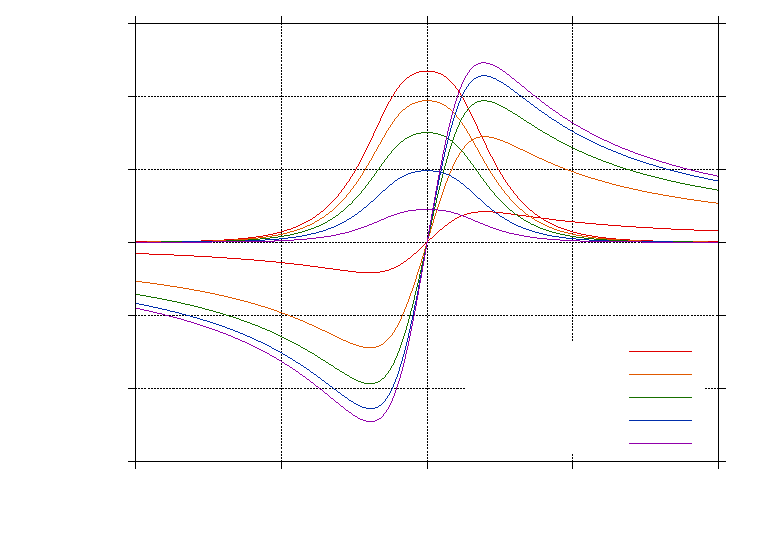
\includegraphics{Figures/twowires/Deltas1/kdepend}}%
    \gplfronttext
  \end{picture}%
\endgroup
  
\caption{The pairings $\Delta^{11}_k$ (odd) and $\Delta^{12}_k$ (even) plotted as a function of $k$ for $\Delta^{12}_k$ imaginary. We see, that the functional behaviour is independent of $d$, and that there is a cross over between interwire and intrawire dominated pairing. The intrawire pairing is increased as $d$ increases. Vice versa for the interwire pairing. Parameters: $(n_Ba_B^3)^{1/3} = 0.01$, $(n_Ba_{BF}^3)^{1/3} = 0.11$, $l_t = 0$, $\frac{m_B}{m_F} = 7/40$, $\frac{n_F}{n_B^{1/3}} = 0.215$, $v_F/c_0 = 0.33$. }  
\label{fig.pairingkdependT0dvaried}  
\end{center}    
\end{figure}

To get a physically clearer picture of the effect of the pairings we calculate the pair wave functions in real space as well. Analogous to the calculation in subsection \ref{subsec.1wirepairwavefunction} we get the pair wave functions:
\begin{align}
\braket{\psi_{1,F}(x)\psi_{1,F}(0)} = - \braket{\psi_{2,F}(x)\psi_{2,F}(0)} &= \frac{i}{\mathcal{L}}\sum_k \sin(kx) \frac{\Delta^{11}_k}{2E_{F,k}}\tanh\left[\frac{ \beta E_{F,k} }{2}\right], \nonumber \\
\braket{\psi_{1,F}(x)\psi_{2,F}(0)} &= \frac{1}{\mathcal{L}}\sum_k \cos(kx) \frac{\Delta^{12}_k}{2E_{F,k}}\tanh\left[\frac{ \beta E_{F,k} }{2}\right].
\label{eq.2wirespairwavefunctionsDelta12imaginary}
\end{align} 
Here we should note, that if $E^\pm_{F,k} \neq E_{F,k}$ then the above pair wave functions will be altered. From this we can infer an overall functional behaviour. Firstly, we see that $\braket{\psi_{1,F}(x)\psi_{1,F}(0)}$ and $\braket{\psi_{1,F}(x)\psi_{2,F}(0)}$ are respectively odd and even in $x$. Further, since $\sin(kx)$ and $\cos(kx)$ oscillates more rapidly as a function of $k$ at higher values of $x$ we expect the pair wave functions to decay to 0. This is also physically reasonable.  

As noted in subsection \ref{subsec.1wirepairwavefunction}, the pair wave function is a measure of the spatial correlations between the fermions. Hence, a high value of $\left|\braket{\psi_{1,F}(x)\psi_{1,F}(0)}\right|$ means, that there is a tendency of two particles in the same wire to have the interparticle distance $x$. Similarly a high value $\left|\braket{\psi_{1,F}(x)\psi_{2,F}(0)}\right|$ means, that if a fermion in wire 2 is located at $x' = 0$, there is a tendency of a second fermion to be located at the position $x$ in wire 1.  

\begin{figure} 
\begin{center}  
% GNUPLOT: LaTeX picture with Postscript
\begingroup
  \makeatletter
  \providecommand\color[2][]{%
    \GenericError{(gnuplot) \space\space\space\@spaces}{%
      Package color not loaded in conjunction with
      terminal option `colourtext'%
    }{See the gnuplot documentation for explanation.%
    }{Either use 'blacktext' in gnuplot or load the package
      color.sty in LaTeX.}%
    \renewcommand\color[2][]{}%
  }%
  \providecommand\includegraphics[2][]{%
    \GenericError{(gnuplot) \space\space\space\@spaces}{%
      Package graphicx or graphics not loaded%
    }{See the gnuplot documentation for explanation.%
    }{The gnuplot epslatex terminal needs graphicx.sty or graphics.sty.}%
    \renewcommand\includegraphics[2][]{}%
  }%
  \providecommand\rotatebox[2]{#2}%
  \@ifundefined{ifGPcolor}{%
    \newif\ifGPcolor
    \GPcolorfalse
  }{}%
  \@ifundefined{ifGPblacktext}{%
    \newif\ifGPblacktext
    \GPblacktexttrue
  }{}%
  % define a \g@addto@macro without @ in the name:
  \let\gplgaddtomacro\g@addto@macro
  % define empty templates for all commands taking text:
  \gdef\gplbacktext{}%
  \gdef\gplfronttext{}%
  \makeatother
  \ifGPblacktext
    % no textcolor at all
    \def\colorrgb#1{}%
    \def\colorgray#1{}%
  \else
    % gray or color?
    \ifGPcolor
      \def\colorrgb#1{\color[rgb]{#1}}%
      \def\colorgray#1{\color[gray]{#1}}%
      \expandafter\def\csname LTw\endcsname{\color{white}}%
      \expandafter\def\csname LTb\endcsname{\color{black}}%
      \expandafter\def\csname LTa\endcsname{\color{black}}%
      \expandafter\def\csname LT0\endcsname{\color[rgb]{1,0,0}}%
      \expandafter\def\csname LT1\endcsname{\color[rgb]{0,1,0}}%
      \expandafter\def\csname LT2\endcsname{\color[rgb]{0,0,1}}%
      \expandafter\def\csname LT3\endcsname{\color[rgb]{1,0,1}}%
      \expandafter\def\csname LT4\endcsname{\color[rgb]{0,1,1}}%
      \expandafter\def\csname LT5\endcsname{\color[rgb]{1,1,0}}%
      \expandafter\def\csname LT6\endcsname{\color[rgb]{0,0,0}}%
      \expandafter\def\csname LT7\endcsname{\color[rgb]{1,0.3,0}}%
      \expandafter\def\csname LT8\endcsname{\color[rgb]{0.5,0.5,0.5}}%
    \else
      % gray
      \def\colorrgb#1{\color{black}}%
      \def\colorgray#1{\color[gray]{#1}}%
      \expandafter\def\csname LTw\endcsname{\color{white}}%
      \expandafter\def\csname LTb\endcsname{\color{black}}%
      \expandafter\def\csname LTa\endcsname{\color{black}}%
      \expandafter\def\csname LT0\endcsname{\color{black}}%
      \expandafter\def\csname LT1\endcsname{\color{black}}%
      \expandafter\def\csname LT2\endcsname{\color{black}}%
      \expandafter\def\csname LT3\endcsname{\color{black}}%
      \expandafter\def\csname LT4\endcsname{\color{black}}%
      \expandafter\def\csname LT5\endcsname{\color{black}}%
      \expandafter\def\csname LT6\endcsname{\color{black}}%
      \expandafter\def\csname LT7\endcsname{\color{black}}%
      \expandafter\def\csname LT8\endcsname{\color{black}}%
    \fi
  \fi
    \setlength{\unitlength}{0.0500bp}%
    \ifx\gptboxheight\undefined%
      \newlength{\gptboxheight}%
      \newlength{\gptboxwidth}%
      \newsavebox{\gptboxtext}%
    \fi%
    \setlength{\fboxrule}{0.5pt}%
    \setlength{\fboxsep}{1pt}%
\begin{picture}(7200.00,5040.00)%
    \gplgaddtomacro\gplbacktext{%
      \csname LTb\endcsname%
      \put(1078,1118){\makebox(0,0)[r]{\strut{}$-0.15$}}%
      \csname LTb\endcsname%
      \put(1078,1702){\makebox(0,0)[r]{\strut{}$-0.1$}}%
      \csname LTb\endcsname%
      \put(1078,2287){\makebox(0,0)[r]{\strut{}$-0.05$}}%
      \csname LTb\endcsname%
      \put(1078,2872){\makebox(0,0)[r]{\strut{}$0$}}%
      \csname LTb\endcsname%
      \put(1078,3456){\makebox(0,0)[r]{\strut{}$0.05$}}%
      \csname LTb\endcsname%
      \put(1078,4041){\makebox(0,0)[r]{\strut{}$0.1$}}%
      \csname LTb\endcsname%
      \put(1078,4625){\makebox(0,0)[r]{\strut{}$0.15$}}%
      \csname LTb\endcsname%
      \put(1273,484){\makebox(0,0){\strut{}$-20$}}%
      \csname LTb\endcsname%
      \put(1956,484){\makebox(0,0){\strut{}$-15$}}%
      \csname LTb\endcsname%
      \put(2640,484){\makebox(0,0){\strut{}$-10$}}%
      \csname LTb\endcsname%
      \put(3323,484){\makebox(0,0){\strut{}$-5$}}%
      \csname LTb\endcsname%
      \put(4007,484){\makebox(0,0){\strut{}$0$}}%
      \csname LTb\endcsname%
      \put(4690,484){\makebox(0,0){\strut{}$5$}}%
      \csname LTb\endcsname%
      \put(5373,484){\makebox(0,0){\strut{}$10$}}%
      \csname LTb\endcsname%
      \put(6057,484){\makebox(0,0){\strut{}$15$}}%
      \csname LTb\endcsname%
      \put(6740,484){\makebox(0,0){\strut{}$20$}}%
    }%
    \gplgaddtomacro\gplfronttext{%
      \csname LTb\endcsname%
      \put(176,2871){\rotatebox{-270}{\makebox(0,0){\strut{}$Pair wave functions$}}}%
      \put(4006,154){\makebox(0,0){\strut{}$k_Fx$}}%
      \csname LTb\endcsname%
      \put(5753,1820){\makebox(0,0)[r]{\strut{}$k_Fd = 0.720$}}%
      \csname LTb\endcsname%
      \put(5753,1600){\makebox(0,0)[r]{\strut{}$k_Fd = 0.735$}}%
      \csname LTb\endcsname%
      \put(5753,1380){\makebox(0,0)[r]{\strut{}$k_Fd = 0.750$}}%
      \csname LTb\endcsname%
      \put(5753,1160){\makebox(0,0)[r]{\strut{}$k_Fd = 0.765$}}%
      \csname LTb\endcsname%
      \put(5753,940){\makebox(0,0)[r]{\strut{}$k_Fd = 0.775$}}%
    }%
    \gplbacktext
    \put(0,0){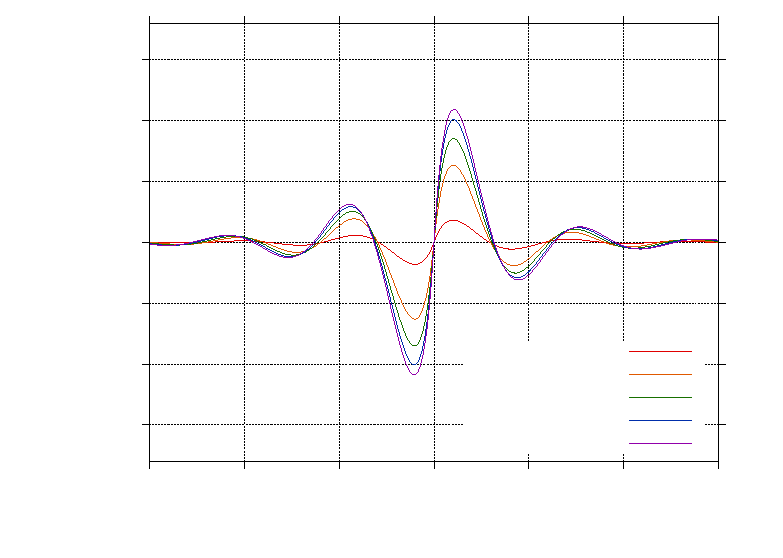
\includegraphics{xdepend11}}%
    \gplfronttext
  \end{picture}%
\endgroup
  
\caption{The \textit{intra}wire pairwave function $\braket{\psi_{1,F}(x)\psi_{1,F}(0)}$ as a function of $x$ for $\Delta^{12}_k$ imaginary. We see, that the functional behaviour is independent of $d$, the pair wave function is simply decreased as $d$ decreases. Parameters: $(n_Ba_B^3)^{1/3} = 0.01$, $(n_Ba_{BF}^3)^{1/3} = 0.11$, $l_t = 0$, $\frac{m_B}{m_F} = 7/40$, $\frac{n_F}{n_B^{1/3}} = 0.215$, $v_F/c_0 = 0.33$. }  
\label{fig.2wirespairwavefunction11}  
\end{center}    
\end{figure}

\begin{figure} 
\begin{center}  
% GNUPLOT: LaTeX picture with Postscript
\begingroup
  \makeatletter
  \providecommand\color[2][]{%
    \GenericError{(gnuplot) \space\space\space\@spaces}{%
      Package color not loaded in conjunction with
      terminal option `colourtext'%
    }{See the gnuplot documentation for explanation.%
    }{Either use 'blacktext' in gnuplot or load the package
      color.sty in LaTeX.}%
    \renewcommand\color[2][]{}%
  }%
  \providecommand\includegraphics[2][]{%
    \GenericError{(gnuplot) \space\space\space\@spaces}{%
      Package graphicx or graphics not loaded%
    }{See the gnuplot documentation for explanation.%
    }{The gnuplot epslatex terminal needs graphicx.sty or graphics.sty.}%
    \renewcommand\includegraphics[2][]{}%
  }%
  \providecommand\rotatebox[2]{#2}%
  \@ifundefined{ifGPcolor}{%
    \newif\ifGPcolor
    \GPcolorfalse
  }{}%
  \@ifundefined{ifGPblacktext}{%
    \newif\ifGPblacktext
    \GPblacktexttrue
  }{}%
  % define a \g@addto@macro without @ in the name:
  \let\gplgaddtomacro\g@addto@macro
  % define empty templates for all commands taking text:
  \gdef\gplbacktext{}%
  \gdef\gplfronttext{}%
  \makeatother
  \ifGPblacktext
    % no textcolor at all
    \def\colorrgb#1{}%
    \def\colorgray#1{}%
  \else
    % gray or color?
    \ifGPcolor
      \def\colorrgb#1{\color[rgb]{#1}}%
      \def\colorgray#1{\color[gray]{#1}}%
      \expandafter\def\csname LTw\endcsname{\color{white}}%
      \expandafter\def\csname LTb\endcsname{\color{black}}%
      \expandafter\def\csname LTa\endcsname{\color{black}}%
      \expandafter\def\csname LT0\endcsname{\color[rgb]{1,0,0}}%
      \expandafter\def\csname LT1\endcsname{\color[rgb]{0,1,0}}%
      \expandafter\def\csname LT2\endcsname{\color[rgb]{0,0,1}}%
      \expandafter\def\csname LT3\endcsname{\color[rgb]{1,0,1}}%
      \expandafter\def\csname LT4\endcsname{\color[rgb]{0,1,1}}%
      \expandafter\def\csname LT5\endcsname{\color[rgb]{1,1,0}}%
      \expandafter\def\csname LT6\endcsname{\color[rgb]{0,0,0}}%
      \expandafter\def\csname LT7\endcsname{\color[rgb]{1,0.3,0}}%
      \expandafter\def\csname LT8\endcsname{\color[rgb]{0.5,0.5,0.5}}%
    \else
      % gray
      \def\colorrgb#1{\color{black}}%
      \def\colorgray#1{\color[gray]{#1}}%
      \expandafter\def\csname LTw\endcsname{\color{white}}%
      \expandafter\def\csname LTb\endcsname{\color{black}}%
      \expandafter\def\csname LTa\endcsname{\color{black}}%
      \expandafter\def\csname LT0\endcsname{\color{black}}%
      \expandafter\def\csname LT1\endcsname{\color{black}}%
      \expandafter\def\csname LT2\endcsname{\color{black}}%
      \expandafter\def\csname LT3\endcsname{\color{black}}%
      \expandafter\def\csname LT4\endcsname{\color{black}}%
      \expandafter\def\csname LT5\endcsname{\color{black}}%
      \expandafter\def\csname LT6\endcsname{\color{black}}%
      \expandafter\def\csname LT7\endcsname{\color{black}}%
      \expandafter\def\csname LT8\endcsname{\color{black}}%
    \fi
  \fi
    \setlength{\unitlength}{0.0500bp}%
    \ifx\gptboxheight\undefined%
      \newlength{\gptboxheight}%
      \newlength{\gptboxwidth}%
      \newsavebox{\gptboxtext}%
    \fi%
    \setlength{\fboxrule}{0.5pt}%
    \setlength{\fboxsep}{1pt}%
\begin{picture}(7200.00,5040.00)%
    \gplgaddtomacro\gplbacktext{%
      \csname LTb\endcsname%
      \put(1078,1118){\makebox(0,0)[r]{\strut{}$-0.15$}}%
      \csname LTb\endcsname%
      \put(1078,1702){\makebox(0,0)[r]{\strut{}$-0.1$}}%
      \csname LTb\endcsname%
      \put(1078,2287){\makebox(0,0)[r]{\strut{}$-0.05$}}%
      \csname LTb\endcsname%
      \put(1078,2872){\makebox(0,0)[r]{\strut{}$0$}}%
      \csname LTb\endcsname%
      \put(1078,3456){\makebox(0,0)[r]{\strut{}$0.05$}}%
      \csname LTb\endcsname%
      \put(1078,4041){\makebox(0,0)[r]{\strut{}$0.1$}}%
      \csname LTb\endcsname%
      \put(1078,4625){\makebox(0,0)[r]{\strut{}$0.15$}}%
      \csname LTb\endcsname%
      \put(1273,484){\makebox(0,0){\strut{}$-20$}}%
      \csname LTb\endcsname%
      \put(1956,484){\makebox(0,0){\strut{}$-15$}}%
      \csname LTb\endcsname%
      \put(2640,484){\makebox(0,0){\strut{}$-10$}}%
      \csname LTb\endcsname%
      \put(3323,484){\makebox(0,0){\strut{}$-5$}}%
      \csname LTb\endcsname%
      \put(4007,484){\makebox(0,0){\strut{}$0$}}%
      \csname LTb\endcsname%
      \put(4690,484){\makebox(0,0){\strut{}$5$}}%
      \csname LTb\endcsname%
      \put(5373,484){\makebox(0,0){\strut{}$10$}}%
      \csname LTb\endcsname%
      \put(6057,484){\makebox(0,0){\strut{}$15$}}%
      \csname LTb\endcsname%
      \put(6740,484){\makebox(0,0){\strut{}$20$}}%
    }%
    \gplgaddtomacro\gplfronttext{%
      \csname LTb\endcsname%
      \put(176,2871){\rotatebox{-270}{\makebox(0,0){\strut{}$Pair wave functions$}}}%
      \put(4006,154){\makebox(0,0){\strut{}$k_Fx$}}%
      \csname LTb\endcsname%
      \put(5753,1820){\makebox(0,0)[r]{\strut{}$k_Fd = 0.720$}}%
      \csname LTb\endcsname%
      \put(5753,1600){\makebox(0,0)[r]{\strut{}$k_Fd = 0.735$}}%
      \csname LTb\endcsname%
      \put(5753,1380){\makebox(0,0)[r]{\strut{}$k_Fd = 0.750$}}%
      \csname LTb\endcsname%
      \put(5753,1160){\makebox(0,0)[r]{\strut{}$k_Fd = 0.765$}}%
      \csname LTb\endcsname%
      \put(5753,940){\makebox(0,0)[r]{\strut{}$k_Fd = 0.775$}}%
    }%
    \gplbacktext
    \put(0,0){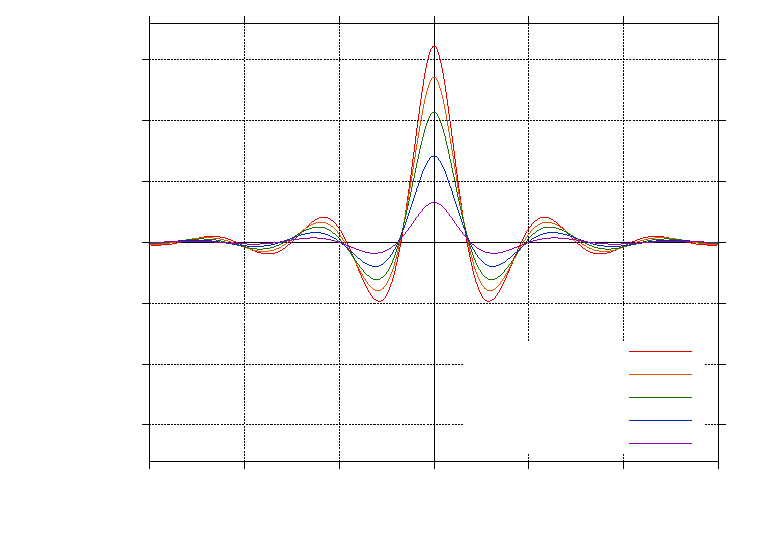
\includegraphics{xdepend12}}%
    \gplfronttext
  \end{picture}%
\endgroup
  
\caption{The \textit{inter}wire pairwave function $\braket{\psi_{1,F}(x)\psi_{2,F}(0)}$ as a function of $x$ for $\Delta^{12}_k$ imaginary. We see, that the functional behaviour is independent of $d$, the pair wave function is simply increased as $d$ decreases. Parameters: $(n_Ba_B^3)^{1/3} = 0.01$, $(n_Ba_{BF}^3)^{1/3} = 0.11$, $l_t = 0$, $\frac{m_B}{m_F} = 7/40$, $\frac{n_F}{n_B^{1/3}} = 0.215$, $v_F/c_0 = 0.33$. }  
\label{fig.2wirespairwavefunction12}  
\end{center}    
\end{figure}

By using the pairings found in the above analysis we can readily calculate the pair wave functions numerically. The result is shown in figures \ref{fig.2wirespairwavefunction11} and \ref{fig.2wirespairwavefunction12}. They have the following physical interpretation. The \textit{intra}wire pair wave function of figure \ref{fig.2wirespairwavefunction11} has the exact same structure as in the single wire case. There is a high tendency of the particles to be a distance $1/k_F$ apart internally in each wire. Further, the correlation is decreased when we decrease the interwire distance, $d$, since the intrawire pairing decreases. The \textit{inter}wire pair wave function of figure \ref{fig.2wirespairwavefunction12}, shows that there is a tendency of a fermion in wire 1 to be facing a fermion in wire 2. As for the single wire case we can come with the following intuitive picture of how the pairings tend to order the system. When the wires are well separated the intrawire pairing dominates the interwire one. This means, that the fermions tend to have an interparticle distance of $1 / k_F$ internally in each wire, but there is no correlation of the positions between the wires. This is illustrated to the left in figure \ref{fig.2wirespositioncorrelations}. For intermediate distances both pairings are present and the system is ordered both with respect to the intrawire and interwire correlations. This is the middle of figure \ref{fig.2wirespositioncorrelations}. Finally for small interwire distances, only the interwire pairing is present: the system only orders with respect to the interwire correlation. 

\begin{figure}
\center
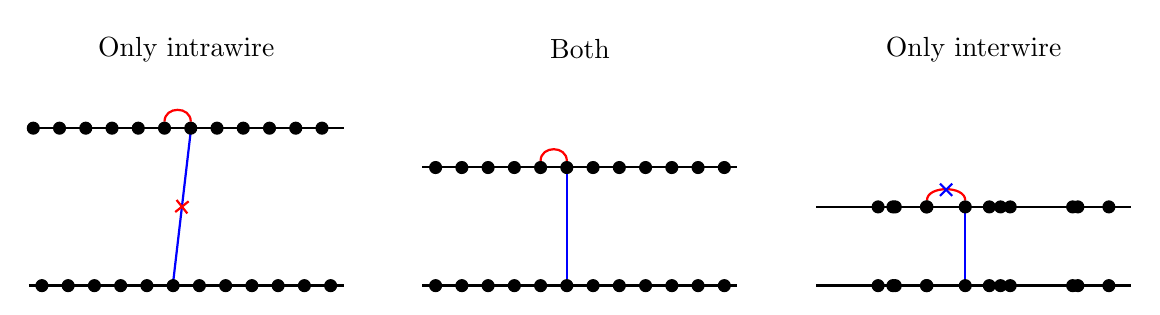
\begin{tikzpicture}

%Only intrawire: 
\node at (2, 3) {Only intrawire};

%correlations:
\draw[-, thick, blue] (6 * 1/3 - 1/6, 0.04) -- (6 * 1/3 - 1/6 + 0.2238, 1.96);  
\draw (6 * 1/3 - 1/6 + 0.1119, 1.0) node[cross, rotate=-6.384836653, thick, red]{}; 
\draw[-, thick, red]  (5 * 1/3 - 1/6 + 0.2238, 2.08) to[out=90, in=90, distance = 0.2cm] (6 * 1/3 - 1/6 + 0.2238, 2.08);

\draw[-, thick] (0, 0) -- (4, 0);
\draw[*-] (1 * 1/3 - 1/6, 0.08); 
\draw[*-] (2 * 1/3 - 1/6, 0.08); 
\draw[*-] (3 * 1/3 - 1/6, 0.08); 
\draw[*-] (4 * 1/3 - 1/6, 0.08); 
\draw[*-] (5 * 1/3 - 1/6, 0.08); 
\draw[*-] (6 * 1/3 - 1/6, 0.08); 
\draw[*-] (7 * 1/3 - 1/6, 0.08); 
\draw[*-] (8 * 1/3 - 1/6, 0.08); 
\draw[*-] (9 * 1/3 - 1/6, 0.08); 
\draw[*-] (10 * 1/3 - 1/6, 0.08); 
\draw[*-] (11 * 1/3 - 1/6, 0.08);
\draw[*-] (12 * 1/3 - 1/6, 0.08); 

\draw[-, thick] (0, 2) -- (4, 2);
\draw[*-] (1 * 1/3 - 1/6 + 0.2238, 2.08); 
\draw[*-] (2 * 1/3 - 1/6 + 0.2238, 2.08); 
\draw[*-] (3 * 1/3 - 1/6 + 0.2238, 2.08); 
\draw[*-] (4 * 1/3 - 1/6 + 0.2238, 2.08); 
\draw[*-] (5 * 1/3 - 1/6 + 0.2238, 2.08); 
\draw[*-] (6 * 1/3 - 1/6 + 0.2238, 2.08); 
\draw[*-] (7 * 1/3 - 1/6 + 0.2238, 2.08); 
\draw[*-] (8 * 1/3 - 1/6 + 0.2238, 2.08); 
\draw[*-] (9 * 1/3 - 1/6 + 0.2238, 2.08); 
\draw[*-] (10 * 1/3 - 1/6 + 0.2238, 2.08); 
\draw[*-] (11 * 1/3 - 1/6 + 0.2238, 2.08);
\draw[*-] (12 * 1/3 - 1/6 + 0.2238 - 4, 2.08);

%%%%%%%%

%BOTH: 
\node at (7, 3) {Both};

%correlations:
\draw[-, thick, blue] (5 + 6 * 1/3 - 1/6, 0.08) -- (5 + 6 * 1/3 - 1/6, 1.58);  
\draw[-, thick, red]  (5 + 5 * 1/3 - 1/6, 1.58) to[out=90, in=90, distance = 0.2cm] (5 + 6 * 1/3 - 1/6, 1.58);

\draw[-, thick] (5, 0) -- (9, 0);
\draw[*-] (1 * 1/3 - 1/6 + 5, 0.08); 
\draw[*-] (2 * 1/3 - 1/6 + 5, 0.08); 
\draw[*-] (3 * 1/3 - 1/6 + 5, 0.08); 
\draw[*-] (4 * 1/3 - 1/6 + 5, 0.08); 
\draw[*-] (5 * 1/3 - 1/6 + 5, 0.08); 
\draw[*-] (6 * 1/3 - 1/6 + 5, 0.08); 
\draw[*-] (7 * 1/3 - 1/6 + 5, 0.08); 
\draw[*-] (8 * 1/3 - 1/6 + 5, 0.08); 
\draw[*-] (9 * 1/3 - 1/6 + 5, 0.08); 
\draw[*-] (10 * 1/3 - 1/6 + 5, 0.08); 
\draw[*-] (11 * 1/3 - 1/6 + 5, 0.08);
\draw[*-] (12 * 1/3 - 1/6 + 5, 0.08);

\draw[-, thick] (5, 1.5) -- (9, 1.5);
\draw[*-] (1 * 1/3 - 1/6 + 5, 1.58); 
\draw[*-] (2 * 1/3 - 1/6 + 5, 1.58); 
\draw[*-] (3 * 1/3 - 1/6 + 5, 1.58); 
\draw[*-] (4 * 1/3 - 1/6 + 5, 1.58); 
\draw[*-] (5 * 1/3 - 1/6 + 5, 1.58); 
\draw[*-] (6 * 1/3 - 1/6 + 5, 1.58); 
\draw[*-] (7 * 1/3 - 1/6 + 5, 1.58); 
\draw[*-] (8 * 1/3 - 1/6 + 5, 1.58); 
\draw[*-] (9 * 1/3 - 1/6 + 5, 1.58); 
\draw[*-] (10 * 1/3 - 1/6 + 5, 1.58); 
\draw[*-] (11 * 1/3 - 1/6 + 5, 1.58);
\draw[*-] (12 * 1/3 - 1/6 + 5, 1.58);

%%%%%%%%

%Only intrawire:
\node at (12, 3) {Only interwire};

%correlations:
\draw[-, thick, blue] (1.8932 + 10, 0.04) -- (1.8932 + 10, 0.96);  
\draw[-, thick, red]  (1.4066 + 10, 1.08) to[out=90, in=90] (1.8932 + 10, 1.08);
\draw (1.4066 + 10 + 0.2433, 1.215) node[cross, thick, blue]{}; 

\draw[-, thick] (10, 0) -- (14, 0);
\draw[*-] (0.7864 + 10, 0.08); 
\draw[*-] (0.9741 + 10, 0.08); 
\draw[*-] (1.0043 + 10, 0.08); 
\draw[*-] (1.3999 + 10, 0.08); 
\draw[*-] (1.4066 + 10, 0.08); 
\draw[*-] (1.8932 + 10, 0.08); 
\draw[*-] (2.1989 + 10, 0.08); 
\draw[*-] (2.3411 + 10, 0.08); 
\draw[*-] (2.4642 + 10, 0.08); 
\draw[*-] (3.2571 + 10, 0.08); 
\draw[*-] (3.3233 + 10, 0.08);
\draw[*-] (3.7171 + 10, 0.08);

\draw[-, thick] (10, 1) -- (14, 1);
\draw[*-] (0.7864 + 10, 1.08); 
\draw[*-] (0.9741 + 10, 1.08); 
\draw[*-] (1.0043 + 10, 1.08); 
\draw[*-] (1.3999 + 10, 1.08); 
\draw[*-] (1.4066 + 10, 1.08); 
\draw[*-] (1.8932 + 10, 1.08); 
\draw[*-] (2.1989 + 10, 1.08); 
\draw[*-] (2.3411 + 10, 1.08); 
\draw[*-] (2.4642 + 10, 1.08); 
\draw[*-] (3.2571 + 10, 1.08); 
\draw[*-] (3.3233 + 10, 1.08);
\draw[*-] (3.7171 + 10, 1.08);

\end{tikzpicture}
\caption{An intuitive picture of how the pairings tend to order the system. The fermions are depicted by black dots. The \textit{intra}wire and \textit{inter}wire correlation is depicted by red and blue lines respectively. Left: large interwire distance; only intrawire pairing present. The intrawire correlation ruins the interwire correlation, hence the red cross over the blue line. Middle: intermediate interwire distance; both pairings present. Both types of correlation are present. Right: small interwire distance; only interwire pairing present. The \textit{inter}wire correlation ruins the intrawire correlation, hence the blue cross over the red line.}
\label{fig.2wirespositioncorrelations}
\end{figure}


We can also use this to come with an intuitive explanation of the uptil now curious fact, that the numerical analysis shows, that the chemical potential is decreased by the presence of the \textit{intra}wire and increased by the presence of the \textit{inter}wire pairing. Specifically at $T = 0$, when only intrawire pairing is present $\mu < \epsilon_{F,0}$ whilst for only interwire pairing: $\mu > \epsilon_{F,0}$. The above analysis shows, that the intrawire pairing makes sure, that the fermions to a higher degree stay out of each others way. Therefore the energy to put in an additional fermion $\mu = \partial E/\partial N_F$ is lowered. Oppositely, the interwire pairing has a tendency to accumulate lumps of fermions, and so the energy required to put in an additional fermion $\mu = \partial E/\partial N_F$ is increased. 

\section{Temperature dependency of pairings} \label{sec.2wirespairingstemperature}
In this section we will investigate, how the pairings depend on temperature. The analysis is performed in complete analogy to the one in subsection \ref{subsec.momentum_and_temperature_pairing_singlewire}. 

For small and large distances, where one of the pairings is dominant, it is not difficult to imagine, what will happen. Here we expect, that the two pairings go to zero in a similar manner to single wire at two different critical temperatures. The dominant pairing for $T = 0$ will have the highest critical temperature. However, a couple questions arise. How does it affect the dominant pairing, that the suppressed pairing goes to zero? And is the interwire or intrawire pairing the more robust to a rise in temperature?

To answer these questions we investigate three cases, two where one pairing is strongly dominant, and one where the pairings are essentially equal for $T = 0$. The more interesting case is definitely the latter one, since this directly tests what pairing is the more robust. However, we might also gain some insight from the former. 

The result of the analysis for a dominant interwire pairing is shown in figure \ref{fig.maximalpairingsTdepend_2wires}. We see, that the overall expected behaviour is observed. We observe that the intrawire pairing has a small downward kink, where the interwire pairing vanishes. The same behaviour is seen when the interwire pairing is dominant. This has to implications. The first is, that the dominant pairing would be higher at low temperatures if the other pairing was not present: there is a trade off between the size of the individual pairings and the presence of a second pairing. The second is, that the presence of a second smaller pairing seem to stabilize the dominant one, since the kink is downwards for increasing temperatures. Further, above the critical temperature of the smaller pairing, the maximal intrawire pairing of the dominating pairing is well described by the following relation:
\begin{equation}
\max_k[\Delta^{\text{dom}}_k(T)] = \alpha \max_k[\Delta^{\text{dom}}_k(T = 0)] \sqrt{1 - \left(\frac{T}{T_c}\right)^3},
\label{eq.DeltaapproxaboveTC1}
\end{equation}
where $\text{dom}$ is short for dominating. This has the same form as the approximate form in equation \eqref{eq.maxpairingapprox} apart from the $\alpha$. The coefficient $\alpha$ is slightly bigger than $1$, but seems to depend slightly on the other parameters of the problem. For the present set of parameters we have $\alpha = 1.3$. 

\begin{figure} 
\begin{center}  
% GNUPLOT: LaTeX picture with Postscript
\begingroup
  \makeatletter
  \providecommand\color[2][]{%
    \GenericError{(gnuplot) \space\space\space\@spaces}{%
      Package color not loaded in conjunction with
      terminal option `colourtext'%
    }{See the gnuplot documentation for explanation.%
    }{Either use 'blacktext' in gnuplot or load the package
      color.sty in LaTeX.}%
    \renewcommand\color[2][]{}%
  }%
  \providecommand\includegraphics[2][]{%
    \GenericError{(gnuplot) \space\space\space\@spaces}{%
      Package graphicx or graphics not loaded%
    }{See the gnuplot documentation for explanation.%
    }{The gnuplot epslatex terminal needs graphicx.sty or graphics.sty.}%
    \renewcommand\includegraphics[2][]{}%
  }%
  \providecommand\rotatebox[2]{#2}%
  \@ifundefined{ifGPcolor}{%
    \newif\ifGPcolor
    \GPcolorfalse
  }{}%
  \@ifundefined{ifGPblacktext}{%
    \newif\ifGPblacktext
    \GPblacktexttrue
  }{}%
  % define a \g@addto@macro without @ in the name:
  \let\gplgaddtomacro\g@addto@macro
  % define empty templates for all commands taking text:
  \gdef\gplbacktext{}%
  \gdef\gplfronttext{}%
  \makeatother
  \ifGPblacktext
    % no textcolor at all
    \def\colorrgb#1{}%
    \def\colorgray#1{}%
  \else
    % gray or color?
    \ifGPcolor
      \def\colorrgb#1{\color[rgb]{#1}}%
      \def\colorgray#1{\color[gray]{#1}}%
      \expandafter\def\csname LTw\endcsname{\color{white}}%
      \expandafter\def\csname LTb\endcsname{\color{black}}%
      \expandafter\def\csname LTa\endcsname{\color{black}}%
      \expandafter\def\csname LT0\endcsname{\color[rgb]{1,0,0}}%
      \expandafter\def\csname LT1\endcsname{\color[rgb]{0,1,0}}%
      \expandafter\def\csname LT2\endcsname{\color[rgb]{0,0,1}}%
      \expandafter\def\csname LT3\endcsname{\color[rgb]{1,0,1}}%
      \expandafter\def\csname LT4\endcsname{\color[rgb]{0,1,1}}%
      \expandafter\def\csname LT5\endcsname{\color[rgb]{1,1,0}}%
      \expandafter\def\csname LT6\endcsname{\color[rgb]{0,0,0}}%
      \expandafter\def\csname LT7\endcsname{\color[rgb]{1,0.3,0}}%
      \expandafter\def\csname LT8\endcsname{\color[rgb]{0.5,0.5,0.5}}%
    \else
      % gray
      \def\colorrgb#1{\color{black}}%
      \def\colorgray#1{\color[gray]{#1}}%
      \expandafter\def\csname LTw\endcsname{\color{white}}%
      \expandafter\def\csname LTb\endcsname{\color{black}}%
      \expandafter\def\csname LTa\endcsname{\color{black}}%
      \expandafter\def\csname LT0\endcsname{\color{black}}%
      \expandafter\def\csname LT1\endcsname{\color{black}}%
      \expandafter\def\csname LT2\endcsname{\color{black}}%
      \expandafter\def\csname LT3\endcsname{\color{black}}%
      \expandafter\def\csname LT4\endcsname{\color{black}}%
      \expandafter\def\csname LT5\endcsname{\color{black}}%
      \expandafter\def\csname LT6\endcsname{\color{black}}%
      \expandafter\def\csname LT7\endcsname{\color{black}}%
      \expandafter\def\csname LT8\endcsname{\color{black}}%
    \fi
  \fi
    \setlength{\unitlength}{0.0500bp}%
    \ifx\gptboxheight\undefined%
      \newlength{\gptboxheight}%
      \newlength{\gptboxwidth}%
      \newsavebox{\gptboxtext}%
    \fi%
    \setlength{\fboxrule}{0.5pt}%
    \setlength{\fboxsep}{1pt}%
\begin{picture}(7200.00,5040.00)%
    \gplgaddtomacro\gplbacktext{%
      \csname LTb\endcsname%
      \put(814,767){\makebox(0,0)[r]{\strut{}$0$}}%
      \csname LTb\endcsname%
      \put(814,1609){\makebox(0,0)[r]{\strut{}$0.1$}}%
      \csname LTb\endcsname%
      \put(814,2451){\makebox(0,0)[r]{\strut{}$0.2$}}%
      \csname LTb\endcsname%
      \put(814,3292){\makebox(0,0)[r]{\strut{}$0.3$}}%
      \csname LTb\endcsname%
      \put(814,4134){\makebox(0,0)[r]{\strut{}$0.4$}}%
      \csname LTb\endcsname%
      \put(814,4976){\makebox(0,0)[r]{\strut{}$0.5$}}%
      \csname LTb\endcsname%
      \put(1009,484){\makebox(0,0){\strut{}$0$}}%
      \csname LTb\endcsname%
      \put(1964,484){\makebox(0,0){\strut{}$0.05$}}%
      \csname LTb\endcsname%
      \put(2919,484){\makebox(0,0){\strut{}$0.1$}}%
      \csname LTb\endcsname%
      \put(3875,484){\makebox(0,0){\strut{}$0.15$}}%
      \csname LTb\endcsname%
      \put(4830,484){\makebox(0,0){\strut{}$0.2$}}%
      \csname LTb\endcsname%
      \put(5785,484){\makebox(0,0){\strut{}$0.25$}}%
      \csname LTb\endcsname%
      \put(6740,484){\makebox(0,0){\strut{}$0.3$}}%
    }%
    \gplgaddtomacro\gplfronttext{%
      \csname LTb\endcsname%
      \put(176,2871){\rotatebox{-270}{\makebox(0,0){\strut{}$\max_k[\Delta_k]/\epsilon_{F,0}$}}}%
      \put(3874,154){\makebox(0,0){\strut{}$T/T_F$}}%
    }%
    \gplbacktext
    \put(0,0){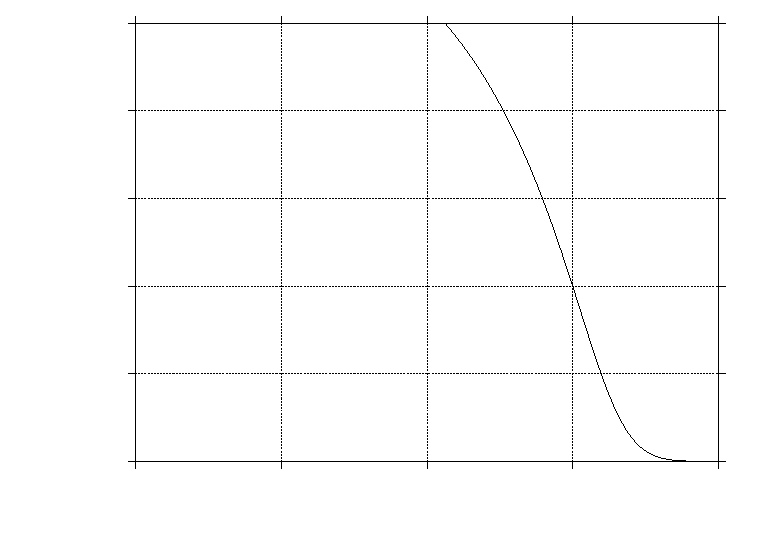
\includegraphics{Figures/twowires/Deltas4.5/Tdepend}}%
    \gplfronttext
  \end{picture}%
\endgroup
  
\caption{Blue solid line: $\max_k[|\Delta^{12}_k|]$ as a function of temperature. Blue dashed line: approximate form from the single wire analysis, equation \eqref{eq.maxpairingapprox}. Red solid line: $\max_k[|\Delta^{11}_k|]$ as a function of temperature. Red dashed line: Approximate form according to equation \eqref{eq.DeltaapproxaboveTC1} above the critical temperature of the interwire pairing. Notice, that there are two critical temperatures, and that the intrawire pairing shows a downward kink, where the interwire pairing goes to zero. Parameters: $k_Fd = 0.61$, $(n_Ba_B^3)^{1/3} = 0.01$, $(n_Ba_{BF}^3)^{1/3} = 0.11$, $l_t = 0$, $\frac{m_B}{m_F} = 7/40$, $\frac{n_F}{n_B^{1/3}} = 0.215$, $v_F/c_0 = 0.33$.}  
\label{fig.maximalpairingsTdepend_2wires}  
\end{center}    
\end{figure} 


\part{Kitaev chain in 1D Bose gas}
In this fourth part..
\newpage
\chapter{Discussion} 

\label{Chapter12} 
\lhead{Part IV. \emph{Discussions \& Conclusions}}
\chead{Chapter 12. \emph{Discussion}} % Change X to a consecutive number; this is for the header on each page - perhaps a shortened title

\section{Cross over in the double wire system and physical discrepancies} \label{sec.Discussion.2wires.crossover}
To have a full understanding of the cross over in the double wire system, we had to use both a bulk and boundary perspective. The bulk effect for the separated wires is, that there is only a topologically nontrivial intrawire $p$-wave pairing present. The resulting boundary effect is, that Majorana edge states can form with no energy cost. Oppositely when the wires are very close, only a topologically trivial interwire $s$-wave pairing is present. In turn there are no edge states. 

To understand the transition inbetween this bulk-boundary correspondence is even more important. As the wires are brought closer together, the interwire interaction respects a time reversal symmetry with $T^2 = - \mathbb{I}$. As the analytical analysis of chapter \ref{Chapter10} shows, the edge states are time reversal (Kramers) partners. Therefore, the edge states are unaffected by the interwire interaction. This holds until a mean field is chosen, namely the interwire $s$-wave pairing. This interwire pairing can do two things through a specific choice of its phase: it can respect the $T^2 = - \mathbb{I}$ symmetry or not. If it respects the symmetry, the edge states are still uncoupled. A calculation of the bulk topological invariant shows, that this holds until the energy gap closes. Then the bulk is topologically trivial and no edge states are present. If it \textit{breaks} this symmetry, the edge states are no longer uncoupled. Actually they gain a nonzero energy for any nonzero interwire pairing. In turn the bulk energy gap does not have to close for the edge state to vanish. 

The nontrivial result of the numerical analysis is, that the interwire pairing chooses to break the $T^2 = -\mathbb{I}$ symmetry. This is simply because it is the energetically favourable choice. Further, a coexistence of the $p$-wave and $s$-wave pairing is observed in the transition. 

This mean field result does however have an important physical discrepancy. Consider the gap equations for the double wire system, equation \eqref{eq.2wiresgapequations}. As we bring the wires closer together the intrawire pairing is not affected by the interwire induced interaction until an interwire pairing forms. This is absurd. The interwire interaction will of course alter the physical properties internally in each wire, also when the wires are far apart. This also leads to the odd prediction, that the critical temperature for intrawire pairing is unaffected by the interwire interaction, as long as the interwire pairing is absent. This is \textit{not} physically reasonable. 

The reason for this discrepancy is the same as the reason why, the mean field approximation breaks down for a single wire above the critical temperature. When no mean field is present, the mean field approximation is the same as neglecting the interaction all together. There is however a way to remedy this (partially) using the socalled self-energy. The self-energy is the energy shift a fermion experiences due to its interaction with all the others. It is clear, that this self-energy will increase as the wires are brought closer together. 

\section{Kitaev chain} \label{sec.Discussion.KitaevChain}
In this thesis we have studied fermionic one-dimensional \textit{gasses}. The original work of Kitaev is based on fermions sitting in a one-dimensional \textit{lattice} with nearest neighbour hopping and pairing \cite{KitaevQuantumWires}. In recent work by Alecce and Dell'Anna an extended version of the Kitaev chain with $r$ neighbours is considered \cite{Alecce.extendKitaev}. They find, that if the hopping and pairing decays sufficiently slow, topological phases with up to $r$ Majorana edge states can be found, hence exceeding the Kitaev result of a single Majorana edge state. 

In this connection we have briefly studied, whether this is possible in our 1D-3D Fermi-Bose mixture. More specifically we think of the fermions as sitting in an optical lattice with nearest and next-nearest neighbour hopping. We must then self-consistently solve for the pairing, $\Delta_k$, and compute the $\mathbb{Z}$-topological invariant $\nu = 2\text{CS}_1$. Since we consider two neighbours, we search for $\nu = \pm 2$. Unfortunately, we have not been able to find such a solution. We speculate, that the reason for this is, that the Yukawa interaction is simply not long range enough. This is supported by the fact, that we can find $\nu = \pm 2$ solutions, when the interaction drops of as $|x|^{-\alpha}$, with $\alpha < 1$. This is also consistent with the findings of Alecce and Dell'Anna. Specifically, they show that the hopping and pairing both have to decay with $\alpha < 1$ for the number of Majorana edge states to exceed 1. This way of producing several edge states systems in the Fermi-Bose mixture framework is therefore considered inapplicable. 



% Chapter 13

\chapter{Numerical analysis} % Main chapter title

\label{Chapter13} % For referencing the chapter elsewhere, use \ref{Chapter12} 

\lhead{Part IV. \emph{Kitaev chain}}
\chead{Chapter 13. \emph{Numerical analysis}} % This is for the header on each page - perhaps a shortened title
%----------------------------------------------------------------------------------------
In this chapter we present the numerical analysis for the Kitaev chain in the one-dimensional Bose gas. In section \ref{sec.onlyNN} we briefly investigate the nearest neighbour hopping only, i.e. $t_2 = 0$. In section \ref{sec.NNNincluded} we include the next-nearest neighbour hopping and study the effect of introducing this parameter. 
 
\section{Only nearest neighbour hopping} \label{sec.onlyNN}
We numerically study the system as a function of two parameters: the coherence length, $\xi$, and the filling fraction $n = N_F/N$. We use the Bose gas parameter $n_Ba_B$ to adjust the coherence length through $\xi \propto (n_Ba_B)^{-1/2}$. We keep the interaction strength, $G$, constant. The phase diagrams are produced in the following manner. For each value of $\xi$ we compute the effective interaction using equation \eqref{eq.gapequation.lattice}. Then for each value of $n$ we come with an initial guess for the pairing. We use $\sin(kd)$, since this is the expected qualitative behaviour. Finally we use equations \eqref{eq.gapequation.lattice} and \eqref{eq.fillingfraction.lattice} to solve for the pairing and chemical potentials in a self-consistent manner for $T = 0$ only. This is done in precisely the same way as in the single and double wire system. This is iterated over $\xi > d$ and $0\leq n \leq 1$. 

The result of the analysis for $G = 4$ and $G = 8$ is shown in figure \ref{fig.phasediagram.t20}. We notice, that the plots are symmetrical around $n = 1/2$ and that a higher interaction strength leads to a narrower window of the topologically nontrivial phase of $\nu = 1$ shown in red. Finally as the coherence length grows, the topological nontrivial phase narrows. We can understand these three effects in the following manner. 

\begin{figure}
\begin{center}
% GNUPLOT: LaTeX picture with Postscript
\begingroup
  \makeatletter
  \providecommand\color[2][]{%
    \GenericError{(gnuplot) \space\space\space\@spaces}{%
      Package color not loaded in conjunction with
      terminal option `colourtext'%
    }{See the gnuplot documentation for explanation.%
    }{Either use 'blacktext' in gnuplot or load the package
      color.sty in LaTeX.}%
    \renewcommand\color[2][]{}%
  }%
  \providecommand\includegraphics[2][]{%
    \GenericError{(gnuplot) \space\space\space\@spaces}{%
      Package graphicx or graphics not loaded%
    }{See the gnuplot documentation for explanation.%
    }{The gnuplot epslatex terminal needs graphicx.sty or graphics.sty.}%
    \renewcommand\includegraphics[2][]{}%
  }%
  \providecommand\rotatebox[2]{#2}%
  \@ifundefined{ifGPcolor}{%
    \newif\ifGPcolor
    \GPcolorfalse
  }{}%
  \@ifundefined{ifGPblacktext}{%
    \newif\ifGPblacktext
    \GPblacktexttrue
  }{}%
  % define a \g@addto@macro without @ in the name:
  \let\gplgaddtomacro\g@addto@macro
  % define empty templates for all commands taking text:
  \gdef\gplbacktext{}%
  \gdef\gplfronttext{}%
  \makeatother
  \ifGPblacktext
    % no textcolor at all
    \def\colorrgb#1{}%
    \def\colorgray#1{}%
  \else
    % gray or color?
    \ifGPcolor
      \def\colorrgb#1{\color[rgb]{#1}}%
      \def\colorgray#1{\color[gray]{#1}}%
      \expandafter\def\csname LTw\endcsname{\color{white}}%
      \expandafter\def\csname LTb\endcsname{\color{black}}%
      \expandafter\def\csname LTa\endcsname{\color{black}}%
      \expandafter\def\csname LT0\endcsname{\color[rgb]{1,0,0}}%
      \expandafter\def\csname LT1\endcsname{\color[rgb]{0,1,0}}%
      \expandafter\def\csname LT2\endcsname{\color[rgb]{0,0,1}}%
      \expandafter\def\csname LT3\endcsname{\color[rgb]{1,0,1}}%
      \expandafter\def\csname LT4\endcsname{\color[rgb]{0,1,1}}%
      \expandafter\def\csname LT5\endcsname{\color[rgb]{1,1,0}}%
      \expandafter\def\csname LT6\endcsname{\color[rgb]{0,0,0}}%
      \expandafter\def\csname LT7\endcsname{\color[rgb]{1,0.3,0}}%
      \expandafter\def\csname LT8\endcsname{\color[rgb]{0.5,0.5,0.5}}%
    \else
      % gray
      \def\colorrgb#1{\color{black}}%
      \def\colorgray#1{\color[gray]{#1}}%
      \expandafter\def\csname LTw\endcsname{\color{white}}%
      \expandafter\def\csname LTb\endcsname{\color{black}}%
      \expandafter\def\csname LTa\endcsname{\color{black}}%
      \expandafter\def\csname LT0\endcsname{\color{black}}%
      \expandafter\def\csname LT1\endcsname{\color{black}}%
      \expandafter\def\csname LT2\endcsname{\color{black}}%
      \expandafter\def\csname LT3\endcsname{\color{black}}%
      \expandafter\def\csname LT4\endcsname{\color{black}}%
      \expandafter\def\csname LT5\endcsname{\color{black}}%
      \expandafter\def\csname LT6\endcsname{\color{black}}%
      \expandafter\def\csname LT7\endcsname{\color{black}}%
      \expandafter\def\csname LT8\endcsname{\color{black}}%
    \fi
  \fi
    \setlength{\unitlength}{0.0500bp}%
    \ifx\gptboxheight\undefined%
      \newlength{\gptboxheight}%
      \newlength{\gptboxwidth}%
      \newsavebox{\gptboxtext}%
    \fi%
    \setlength{\fboxrule}{0.5pt}%
    \setlength{\fboxsep}{1pt}%
\begin{picture}(7200.00,5040.00)%
    \gplgaddtomacro\gplbacktext{%
      \csname LTb\endcsname%
      \put(165,756){\makebox(0,0)[r]{\strut{}$1$}}%
      \put(165,1386){\makebox(0,0)[r]{\strut{}$2$}}%
      \put(165,2016){\makebox(0,0)[r]{\strut{}$3$}}%
      \put(165,2646){\makebox(0,0)[r]{\strut{}$4$}}%
      \put(165,3275){\makebox(0,0)[r]{\strut{}$5$}}%
      \put(165,3905){\makebox(0,0)[r]{\strut{}$6$}}%
      \put(165,4535){\makebox(0,0)[r]{\strut{}$7$}}%
      \put(360,473){\makebox(0,0){\strut{}$0$}}%
      \put(972,473){\makebox(0,0){\strut{}$0.2$}}%
      \put(1584,473){\makebox(0,0){\strut{}$0.4$}}%
      \put(2195,473){\makebox(0,0){\strut{}$0.6$}}%
      \put(2807,473){\makebox(0,0){\strut{}$0.8$}}%
      \put(3419,473){\makebox(0,0){\strut{}$1$}}%
    }%
    \gplgaddtomacro\gplfronttext{%
      \csname LTb\endcsname%
      \put(-209,2645){\rotatebox{-270}{\makebox(0,0){\strut{}$\xi / d$}}}%
      \put(1889,143){\makebox(0,0){\strut{}$n$}}%
      \put(1889,4928){\makebox(0,0){\strut{}$G = 4$}}%
    }%
    \gplgaddtomacro\gplbacktext{%
      \csname LTb\endcsname%
      \put(3584,756){\makebox(0,0)[r]{\strut{} }}%
      \put(3584,1386){\makebox(0,0)[r]{\strut{} }}%
      \put(3584,2016){\makebox(0,0)[r]{\strut{} }}%
      \put(3584,2646){\makebox(0,0)[r]{\strut{} }}%
      \put(3584,3275){\makebox(0,0)[r]{\strut{} }}%
      \put(3584,3905){\makebox(0,0)[r]{\strut{} }}%
      \put(3584,4535){\makebox(0,0)[r]{\strut{} }}%
      \put(3779,473){\makebox(0,0){\strut{}$0$}}%
      \put(4391,473){\makebox(0,0){\strut{}$0.2$}}%
      \put(5003,473){\makebox(0,0){\strut{}$0.4$}}%
      \put(5615,473){\makebox(0,0){\strut{}$0.6$}}%
      \put(6227,473){\makebox(0,0){\strut{}$0.8$}}%
      \put(6839,473){\makebox(0,0){\strut{}$1$}}%
    }%
    \gplgaddtomacro\gplfronttext{%
      \csname LTb\endcsname%
      \put(5309,143){\makebox(0,0){\strut{}$n$}}%
      \put(5309,4928){\makebox(0,0){\strut{}$G = 8$}}%
    }%
    \gplbacktext
    \put(0,0){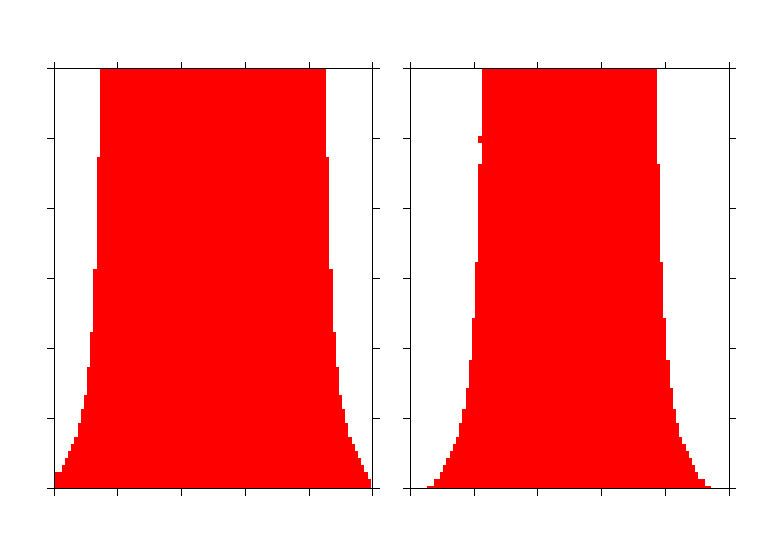
\includegraphics{Figures/Lattice.singlewire/Delta0.0/xifilldepend}}%
    \gplfronttext
  \end{picture}%
\endgroup

\caption{Phase diagrams for $G = 4$ and $G = 8$ as a function of the filling fraction $n = N_F/N$ and the coherence length $\xi$. In white: $\nu = 0$. In red: $\nu = 1$. We notice that the phase diagram for a stronger interaction exhibits a narrower window of topological nontrivial $\nu = 1$. Number of sites: $N = 100$. }
\label{fig.phasediagram.t20}
\end{center}
\end{figure}

First, the symmetry around $n = 1/2$ was discussed in section \ref{sec.fillingfractionsymmetry.breakdown}. Here we showed, that letting $n\to 1 - n$ is a symmetry of the system, if we let $\mu \to -\mu$ and $\Delta_{k} \to \Delta_{k + \pi/d}$. The topological invariant is protected under this symmetry for the following two reasons. Firstly, if $\varepsilon_k(\mu) = -t_1\cos(kd) - \mu$ crosses zero, then so does $\varepsilon_k(-\mu)$. Further, the pairing is simply shifted by $\pi / d$. This means, that there is still a contribution of $\text{sgn}(\Delta_{k_1+\pi/d})$ to the invariant from the zero of $\varepsilon_k$ in $k_1$.

Secondly, for a stronger interaction strength, $G$, the window of the topological phase narrows. The reason is, that when there is a nonzero interaction, the band $-t_1\cos(kd)$ can be populated eventhough $\mu$ is below the minimum of the band, i.e. $\mu < -t_1$. For a stronger interaction still, this population starts for lower and lower $\mu$ and there is a larger and larger region, where $\varepsilon_k = -t_1\cos(kd) - \mu$ is strictly positive. This is the topologically trivial region, which hereby becomes larger. The argument for the coherence length follows the same logic.

The effects of higher interaction strength and longer coherence length are the same at $n$ and $1 - n$, because of the filling fraction symmetry. They can be confirmed by studying the dependency $\mu(n)$, e.g. for $G = 0, G = 4$ and $G = 8$. This results in figure \ref{fig.mun.t20.Gdepend}. We clearly observe a nonzero population in the regions with $|\mu| > t_1$ for nonzero interactions, and an increase in the size of these regions with increasing interaction strength. Studying the effect of an increase in $\xi$ confirms, that the effect hereof is essentially the same as increasing the strength, $G$.  

\begin{figure}
\begin{center}
% GNUPLOT: LaTeX picture with Postscript
\begingroup
  \makeatletter
  \providecommand\color[2][]{%
    \GenericError{(gnuplot) \space\space\space\@spaces}{%
      Package color not loaded in conjunction with
      terminal option `colourtext'%
    }{See the gnuplot documentation for explanation.%
    }{Either use 'blacktext' in gnuplot or load the package
      color.sty in LaTeX.}%
    \renewcommand\color[2][]{}%
  }%
  \providecommand\includegraphics[2][]{%
    \GenericError{(gnuplot) \space\space\space\@spaces}{%
      Package graphicx or graphics not loaded%
    }{See the gnuplot documentation for explanation.%
    }{The gnuplot epslatex terminal needs graphicx.sty or graphics.sty.}%
    \renewcommand\includegraphics[2][]{}%
  }%
  \providecommand\rotatebox[2]{#2}%
  \@ifundefined{ifGPcolor}{%
    \newif\ifGPcolor
    \GPcolorfalse
  }{}%
  \@ifundefined{ifGPblacktext}{%
    \newif\ifGPblacktext
    \GPblacktexttrue
  }{}%
  % define a \g@addto@macro without @ in the name:
  \let\gplgaddtomacro\g@addto@macro
  % define empty templates for all commands taking text:
  \gdef\gplbacktext{}%
  \gdef\gplfronttext{}%
  \makeatother
  \ifGPblacktext
    % no textcolor at all
    \def\colorrgb#1{}%
    \def\colorgray#1{}%
  \else
    % gray or color?
    \ifGPcolor
      \def\colorrgb#1{\color[rgb]{#1}}%
      \def\colorgray#1{\color[gray]{#1}}%
      \expandafter\def\csname LTw\endcsname{\color{white}}%
      \expandafter\def\csname LTb\endcsname{\color{black}}%
      \expandafter\def\csname LTa\endcsname{\color{black}}%
      \expandafter\def\csname LT0\endcsname{\color[rgb]{1,0,0}}%
      \expandafter\def\csname LT1\endcsname{\color[rgb]{0,1,0}}%
      \expandafter\def\csname LT2\endcsname{\color[rgb]{0,0,1}}%
      \expandafter\def\csname LT3\endcsname{\color[rgb]{1,0,1}}%
      \expandafter\def\csname LT4\endcsname{\color[rgb]{0,1,1}}%
      \expandafter\def\csname LT5\endcsname{\color[rgb]{1,1,0}}%
      \expandafter\def\csname LT6\endcsname{\color[rgb]{0,0,0}}%
      \expandafter\def\csname LT7\endcsname{\color[rgb]{1,0.3,0}}%
      \expandafter\def\csname LT8\endcsname{\color[rgb]{0.5,0.5,0.5}}%
    \else
      % gray
      \def\colorrgb#1{\color{black}}%
      \def\colorgray#1{\color[gray]{#1}}%
      \expandafter\def\csname LTw\endcsname{\color{white}}%
      \expandafter\def\csname LTb\endcsname{\color{black}}%
      \expandafter\def\csname LTa\endcsname{\color{black}}%
      \expandafter\def\csname LT0\endcsname{\color{black}}%
      \expandafter\def\csname LT1\endcsname{\color{black}}%
      \expandafter\def\csname LT2\endcsname{\color{black}}%
      \expandafter\def\csname LT3\endcsname{\color{black}}%
      \expandafter\def\csname LT4\endcsname{\color{black}}%
      \expandafter\def\csname LT5\endcsname{\color{black}}%
      \expandafter\def\csname LT6\endcsname{\color{black}}%
      \expandafter\def\csname LT7\endcsname{\color{black}}%
      \expandafter\def\csname LT8\endcsname{\color{black}}%
    \fi
  \fi
    \setlength{\unitlength}{0.0500bp}%
    \ifx\gptboxheight\undefined%
      \newlength{\gptboxheight}%
      \newlength{\gptboxwidth}%
      \newsavebox{\gptboxtext}%
    \fi%
    \setlength{\fboxrule}{0.5pt}%
    \setlength{\fboxsep}{1pt}%
\begin{picture}(7200.00,5040.00)%
    \gplgaddtomacro\gplbacktext{%
      \csname LTb\endcsname%
      \put(682,1188){\makebox(0,0)[r]{\strut{}$-2$}}%
      \csname LTb\endcsname%
      \put(682,2030){\makebox(0,0)[r]{\strut{}$-1$}}%
      \csname LTb\endcsname%
      \put(682,2872){\makebox(0,0)[r]{\strut{}$0$}}%
      \csname LTb\endcsname%
      \put(682,3713){\makebox(0,0)[r]{\strut{}$1$}}%
      \csname LTb\endcsname%
      \put(682,4555){\makebox(0,0)[r]{\strut{}$2$}}%
      \csname LTb\endcsname%
      \put(877,484){\makebox(0,0){\strut{}$0$}}%
      \csname LTb\endcsname%
      \put(2050,484){\makebox(0,0){\strut{}$0.2$}}%
      \csname LTb\endcsname%
      \put(3222,484){\makebox(0,0){\strut{}$0.4$}}%
      \csname LTb\endcsname%
      \put(4395,484){\makebox(0,0){\strut{}$0.6$}}%
      \csname LTb\endcsname%
      \put(5567,484){\makebox(0,0){\strut{}$0.8$}}%
      \csname LTb\endcsname%
      \put(6740,484){\makebox(0,0){\strut{}$1$}}%
    }%
    \gplgaddtomacro\gplfronttext{%
      \csname LTb\endcsname%
      \put(176,2871){\rotatebox{-270}{\makebox(0,0){\strut{}$\mu$}}}%
      \put(3808,154){\makebox(0,0){\strut{}$n$}}%
      \csname LTb\endcsname%
      \put(1933,4803){\makebox(0,0)[r]{\strut{}$G = 0.0$}}%
      \csname LTb\endcsname%
      \put(1933,4583){\makebox(0,0)[r]{\strut{}$G = 2.0$}}%
      \csname LTb\endcsname%
      \put(1933,4363){\makebox(0,0)[r]{\strut{}$G = 4.0$}}%
      \csname LTb\endcsname%
      \put(1933,4143){\makebox(0,0)[r]{\strut{}$G = 8.0$}}%
    }%
    \gplbacktext
    \put(0,0){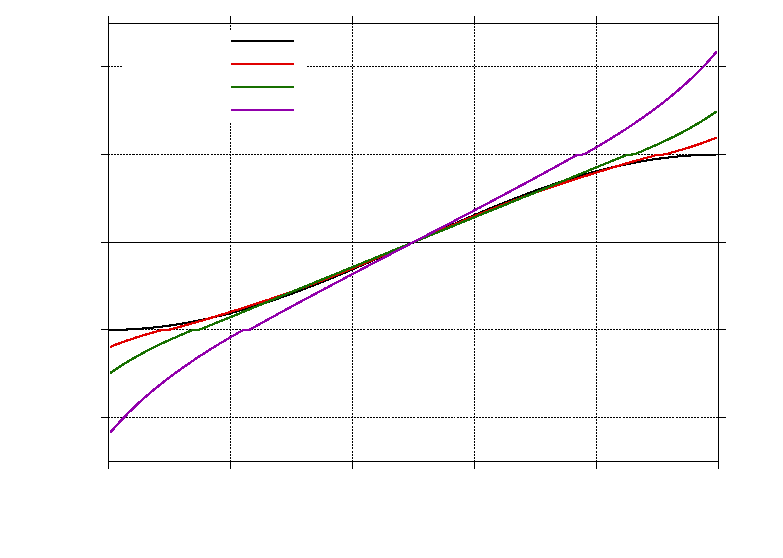
\includegraphics{Figures/Lattice.singlewire/Delta.mu.n0Gvary/ndepend}}%
    \gplfronttext
  \end{picture}%
\endgroup

\caption{The chemical potential, $\mu$, as a function of filling fraction, $n$, for different interaction strengths, $G$. We notice, that for nonzero interaction strengths the lattice starts populating for $|\mu| > t_1$. There is a topological phase transition exactly at $|\mu| = t_1$. $\nu = 1$ for $|\mu|< t_1$ and $\nu = 0$ for $|\mu| > t_1$. Other parameters: $N = 100, \xi / d = 5.0$}
\label{fig.mun.t20.Gdepend}
\end{center}
\end{figure}

\section{Next-nearest neighbour hopping included}
\label{sec.NNNincluded} 

\begin{figure}
\begin{center}
% GNUPLOT: LaTeX picture with Postscript
\begingroup
  \makeatletter
  \providecommand\color[2][]{%
    \GenericError{(gnuplot) \space\space\space\@spaces}{%
      Package color not loaded in conjunction with
      terminal option `colourtext'%
    }{See the gnuplot documentation for explanation.%
    }{Either use 'blacktext' in gnuplot or load the package
      color.sty in LaTeX.}%
    \renewcommand\color[2][]{}%
  }%
  \providecommand\includegraphics[2][]{%
    \GenericError{(gnuplot) \space\space\space\@spaces}{%
      Package graphicx or graphics not loaded%
    }{See the gnuplot documentation for explanation.%
    }{The gnuplot epslatex terminal needs graphicx.sty or graphics.sty.}%
    \renewcommand\includegraphics[2][]{}%
  }%
  \providecommand\rotatebox[2]{#2}%
  \@ifundefined{ifGPcolor}{%
    \newif\ifGPcolor
    \GPcolorfalse
  }{}%
  \@ifundefined{ifGPblacktext}{%
    \newif\ifGPblacktext
    \GPblacktexttrue
  }{}%
  % define a \g@addto@macro without @ in the name:
  \let\gplgaddtomacro\g@addto@macro
  % define empty templates for all commands taking text:
  \gdef\gplbacktext{}%
  \gdef\gplfronttext{}%
  \makeatother
  \ifGPblacktext
    % no textcolor at all
    \def\colorrgb#1{}%
    \def\colorgray#1{}%
  \else
    % gray or color?
    \ifGPcolor
      \def\colorrgb#1{\color[rgb]{#1}}%
      \def\colorgray#1{\color[gray]{#1}}%
      \expandafter\def\csname LTw\endcsname{\color{white}}%
      \expandafter\def\csname LTb\endcsname{\color{black}}%
      \expandafter\def\csname LTa\endcsname{\color{black}}%
      \expandafter\def\csname LT0\endcsname{\color[rgb]{1,0,0}}%
      \expandafter\def\csname LT1\endcsname{\color[rgb]{0,1,0}}%
      \expandafter\def\csname LT2\endcsname{\color[rgb]{0,0,1}}%
      \expandafter\def\csname LT3\endcsname{\color[rgb]{1,0,1}}%
      \expandafter\def\csname LT4\endcsname{\color[rgb]{0,1,1}}%
      \expandafter\def\csname LT5\endcsname{\color[rgb]{1,1,0}}%
      \expandafter\def\csname LT6\endcsname{\color[rgb]{0,0,0}}%
      \expandafter\def\csname LT7\endcsname{\color[rgb]{1,0.3,0}}%
      \expandafter\def\csname LT8\endcsname{\color[rgb]{0.5,0.5,0.5}}%
    \else
      % gray
      \def\colorrgb#1{\color{black}}%
      \def\colorgray#1{\color[gray]{#1}}%
      \expandafter\def\csname LTw\endcsname{\color{white}}%
      \expandafter\def\csname LTb\endcsname{\color{black}}%
      \expandafter\def\csname LTa\endcsname{\color{black}}%
      \expandafter\def\csname LT0\endcsname{\color{black}}%
      \expandafter\def\csname LT1\endcsname{\color{black}}%
      \expandafter\def\csname LT2\endcsname{\color{black}}%
      \expandafter\def\csname LT3\endcsname{\color{black}}%
      \expandafter\def\csname LT4\endcsname{\color{black}}%
      \expandafter\def\csname LT5\endcsname{\color{black}}%
      \expandafter\def\csname LT6\endcsname{\color{black}}%
      \expandafter\def\csname LT7\endcsname{\color{black}}%
      \expandafter\def\csname LT8\endcsname{\color{black}}%
    \fi
  \fi
    \setlength{\unitlength}{0.0500bp}%
    \ifx\gptboxheight\undefined%
      \newlength{\gptboxheight}%
      \newlength{\gptboxwidth}%
      \newsavebox{\gptboxtext}%
    \fi%
    \setlength{\fboxrule}{0.5pt}%
    \setlength{\fboxsep}{1pt}%
\begin{picture}(7200.00,5040.00)%
    \gplgaddtomacro\gplbacktext{%
      \csname LTb\endcsname%
      \put(165,756){\makebox(0,0)[r]{\strut{}$1$}}%
      \put(165,1386){\makebox(0,0)[r]{\strut{}$2$}}%
      \put(165,2016){\makebox(0,0)[r]{\strut{}$3$}}%
      \put(165,2646){\makebox(0,0)[r]{\strut{}$4$}}%
      \put(165,3275){\makebox(0,0)[r]{\strut{}$5$}}%
      \put(165,3905){\makebox(0,0)[r]{\strut{}$6$}}%
      \put(165,4535){\makebox(0,0)[r]{\strut{}$7$}}%
      \put(360,473){\makebox(0,0){\strut{}$0$}}%
      \put(972,473){\makebox(0,0){\strut{}$0.2$}}%
      \put(1584,473){\makebox(0,0){\strut{}$0.4$}}%
      \put(2195,473){\makebox(0,0){\strut{}$0.6$}}%
      \put(2807,473){\makebox(0,0){\strut{}$0.8$}}%
      \put(3419,473){\makebox(0,0){\strut{}$1$}}%
    }%
    \gplgaddtomacro\gplfronttext{%
      \csname LTb\endcsname%
      \put(-209,2645){\rotatebox{-270}{\makebox(0,0){\strut{}$\xi / d$}}}%
      \put(1889,143){\makebox(0,0){\strut{}$n$}}%
      \put(1889,4928){\makebox(0,0){\strut{}$t_2 = t_1, \text{anomalous}$}}%
      \put(972,3590){\makebox(0,0){\color{white}\strut{}$\nu = 1$}}%
      \put(1889, 3590){\makebox(0,0){\color{white}\strut{}$\nu = 2$}}%
      \put(2807,3590){\makebox(0,0){\strut{}$\nu = 0$}}%
      \put(972,3275){\makebox(0,0){\color{white}\strut{}$\times$}}%
      \put(1890,3275){\makebox(0,0){\color{white}\strut{}$*$}}%
    }%
    \gplgaddtomacro\gplbacktext{%
      \csname LTb\endcsname%
      \put(3584,756){\makebox(0,0)[r]{\strut{} }}%
      \put(3584,1386){\makebox(0,0)[r]{\strut{} }}%
      \put(3584,2016){\makebox(0,0)[r]{\strut{} }}%
      \put(3584,2646){\makebox(0,0)[r]{\strut{} }}%
      \put(3584,3275){\makebox(0,0)[r]{\strut{} }}%
      \put(3584,3905){\makebox(0,0)[r]{\strut{} }}%
      \put(3584,4535){\makebox(0,0)[r]{\strut{} }}%
      \put(3779,473){\makebox(0,0){\strut{}$0$}}%
      \put(4391,473){\makebox(0,0){\strut{}$0.2$}}%
      \put(5003,473){\makebox(0,0){\strut{}$0.4$}}%
      \put(5615,473){\makebox(0,0){\strut{}$0.6$}}%
      \put(6227,473){\makebox(0,0){\strut{}$0.8$}}%
      \put(6839,473){\makebox(0,0){\strut{}$1$}}%
    }%
    \gplgaddtomacro\gplfronttext{%
      \csname LTb\endcsname%
      \put(5309,143){\makebox(0,0){\strut{}$n$}}%
      \put(5309,4928){\makebox(0,0){\strut{}$t_2 = t_1, \text{normal}$}}%
      \put(4391,3590){\makebox(0,0){\color{white}\strut{}$\nu = 1$}}%
      \put(6227,3590){\makebox(0,0){\strut{}$\nu = 0$}}%
      \put(4391,3275){\makebox(0,0){\color{white}\strut{}$\times$}}%
      \put(5309,3275){\makebox(0,0){\strut{}$*$}}%
    }%
    \gplbacktext
    \put(0,0){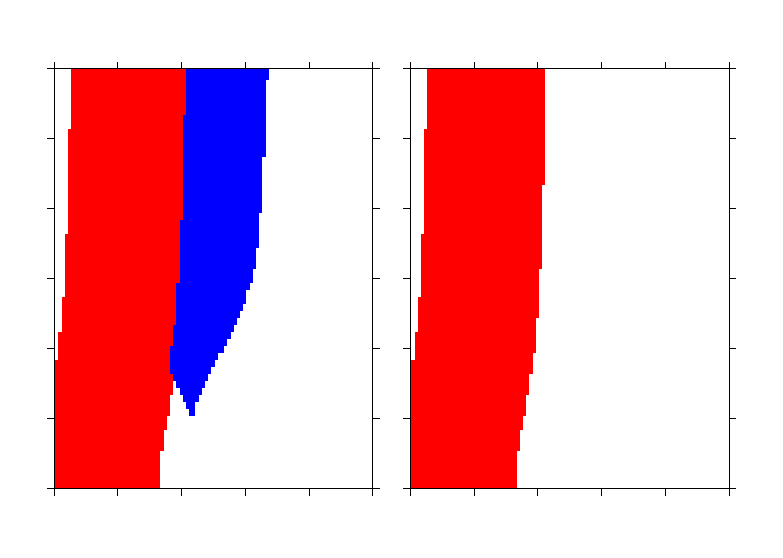
\includegraphics{Figures/Lattice.singlewire/t2nonzerophasediagrams/xifilldepend1}}%
    \gplfronttext
  \end{picture}%
\endgroup

\caption{Topological phase diagram for $t_2 = t_1$ as a function of the filling fraction $n = N_F/N$ and coherence length $\xi$. Invariant: in white: $\nu = 0$, in red: $\nu = 1$, in blue: $\nu = 2$. For points $(i)$ and $(ii)$: see figure \ref{fig.Deltaexamples.t21.0}. To the left: (anomalous) result of searching for $\Delta_k\propto \sin(2kd)$-like solutions. To the right: (normal) result of searching for $\Delta_k \propto \sin(kd)$-like solutions. The algorithm is a little uncertain around the blue tip at $n \approx 0.4, \xi / d \approx 2$. The phase has here been checked by doubling the number of lattice sites. Other parameters: $G = 4$, $N = 100$. }
\label{fig.phasediagram.t21.0}
\vspace{0.5cm}
% GNUPLOT: LaTeX picture with Postscript
\begingroup
  \makeatletter
  \providecommand\color[2][]{%
    \GenericError{(gnuplot) \space\space\space\@spaces}{%
      Package color not loaded in conjunction with
      terminal option `colourtext'%
    }{See the gnuplot documentation for explanation.%
    }{Either use 'blacktext' in gnuplot or load the package
      color.sty in LaTeX.}%
    \renewcommand\color[2][]{}%
  }%
  \providecommand\includegraphics[2][]{%
    \GenericError{(gnuplot) \space\space\space\@spaces}{%
      Package graphicx or graphics not loaded%
    }{See the gnuplot documentation for explanation.%
    }{The gnuplot epslatex terminal needs graphicx.sty or graphics.sty.}%
    \renewcommand\includegraphics[2][]{}%
  }%
  \providecommand\rotatebox[2]{#2}%
  \@ifundefined{ifGPcolor}{%
    \newif\ifGPcolor
    \GPcolorfalse
  }{}%
  \@ifundefined{ifGPblacktext}{%
    \newif\ifGPblacktext
    \GPblacktexttrue
  }{}%
  % define a \g@addto@macro without @ in the name:
  \let\gplgaddtomacro\g@addto@macro
  % define empty templates for all commands taking text:
  \gdef\gplbacktext{}%
  \gdef\gplfronttext{}%
  \makeatother
  \ifGPblacktext
    % no textcolor at all
    \def\colorrgb#1{}%
    \def\colorgray#1{}%
  \else
    % gray or color?
    \ifGPcolor
      \def\colorrgb#1{\color[rgb]{#1}}%
      \def\colorgray#1{\color[gray]{#1}}%
      \expandafter\def\csname LTw\endcsname{\color{white}}%
      \expandafter\def\csname LTb\endcsname{\color{black}}%
      \expandafter\def\csname LTa\endcsname{\color{black}}%
      \expandafter\def\csname LT0\endcsname{\color[rgb]{1,0,0}}%
      \expandafter\def\csname LT1\endcsname{\color[rgb]{0,1,0}}%
      \expandafter\def\csname LT2\endcsname{\color[rgb]{0,0,1}}%
      \expandafter\def\csname LT3\endcsname{\color[rgb]{1,0,1}}%
      \expandafter\def\csname LT4\endcsname{\color[rgb]{0,1,1}}%
      \expandafter\def\csname LT5\endcsname{\color[rgb]{1,1,0}}%
      \expandafter\def\csname LT6\endcsname{\color[rgb]{0,0,0}}%
      \expandafter\def\csname LT7\endcsname{\color[rgb]{1,0.3,0}}%
      \expandafter\def\csname LT8\endcsname{\color[rgb]{0.5,0.5,0.5}}%
    \else
      % gray
      \def\colorrgb#1{\color{black}}%
      \def\colorgray#1{\color[gray]{#1}}%
      \expandafter\def\csname LTw\endcsname{\color{white}}%
      \expandafter\def\csname LTb\endcsname{\color{black}}%
      \expandafter\def\csname LTa\endcsname{\color{black}}%
      \expandafter\def\csname LT0\endcsname{\color{black}}%
      \expandafter\def\csname LT1\endcsname{\color{black}}%
      \expandafter\def\csname LT2\endcsname{\color{black}}%
      \expandafter\def\csname LT3\endcsname{\color{black}}%
      \expandafter\def\csname LT4\endcsname{\color{black}}%
      \expandafter\def\csname LT5\endcsname{\color{black}}%
      \expandafter\def\csname LT6\endcsname{\color{black}}%
      \expandafter\def\csname LT7\endcsname{\color{black}}%
      \expandafter\def\csname LT8\endcsname{\color{black}}%
    \fi
  \fi
    \setlength{\unitlength}{0.0500bp}%
    \ifx\gptboxheight\undefined%
      \newlength{\gptboxheight}%
      \newlength{\gptboxwidth}%
      \newsavebox{\gptboxtext}%
    \fi%
    \setlength{\fboxrule}{0.5pt}%
    \setlength{\fboxsep}{1pt}%
\begin{picture}(7200.00,5040.00)%
    \gplgaddtomacro\gplbacktext{%
      \csname LTb\endcsname%
      \put(165,756){\makebox(0,0)[r]{\strut{}$1$}}%
      \put(165,1386){\makebox(0,0)[r]{\strut{}$2$}}%
      \put(165,2016){\makebox(0,0)[r]{\strut{}$3$}}%
      \put(165,2646){\makebox(0,0)[r]{\strut{}$4$}}%
      \put(165,3275){\makebox(0,0)[r]{\strut{}$5$}}%
      \put(165,3905){\makebox(0,0)[r]{\strut{}$6$}}%
      \put(165,4535){\makebox(0,0)[r]{\strut{}$7$}}%
      \put(360,473){\makebox(0,0){\strut{}$0$}}%
      \put(972,473){\makebox(0,0){\strut{}$0.2$}}%
      \put(1584,473){\makebox(0,0){\strut{}$0.4$}}%
      \put(2195,473){\makebox(0,0){\strut{}$0.6$}}%
      \put(2807,473){\makebox(0,0){\strut{}$0.8$}}%
      \put(3419,473){\makebox(0,0){\strut{}$1$}}%
    }%
    \gplgaddtomacro\gplfronttext{%
      \csname LTb\endcsname%
      \put(-209,2645){\rotatebox{-270}{\makebox(0,0){\strut{}$\xi / d$}}}%
      \put(1889,143){\makebox(0,0){\strut{}$n$}}%
      \put(1889,4928){\makebox(0,0){\strut{}$t_2 = 0.63t_1, \text{anomalous}$}}%
    }%
    \gplgaddtomacro\gplbacktext{%
      \csname LTb\endcsname%
      \put(3584,756){\makebox(0,0)[r]{\strut{} }}%
      \put(3584,1386){\makebox(0,0)[r]{\strut{} }}%
      \put(3584,2016){\makebox(0,0)[r]{\strut{} }}%
      \put(3584,2646){\makebox(0,0)[r]{\strut{} }}%
      \put(3584,3275){\makebox(0,0)[r]{\strut{} }}%
      \put(3584,3905){\makebox(0,0)[r]{\strut{} }}%
      \put(3584,4535){\makebox(0,0)[r]{\strut{} }}%
      \put(3779,473){\makebox(0,0){\strut{}$0$}}%
      \put(4391,473){\makebox(0,0){\strut{}$0.2$}}%
      \put(5003,473){\makebox(0,0){\strut{}$0.4$}}%
      \put(5615,473){\makebox(0,0){\strut{}$0.6$}}%
      \put(6227,473){\makebox(0,0){\strut{}$0.8$}}%
      \put(6839,473){\makebox(0,0){\strut{}$1$}}%
    }%
    \gplgaddtomacro\gplfronttext{%
      \csname LTb\endcsname%
      \put(5309,143){\makebox(0,0){\strut{}$n$}}%
      \put(5309,4928){\makebox(0,0){\strut{}$t_2 = 0.63t_1, \text{normal}$}}%
    }%
    \gplbacktext
    \put(0,0){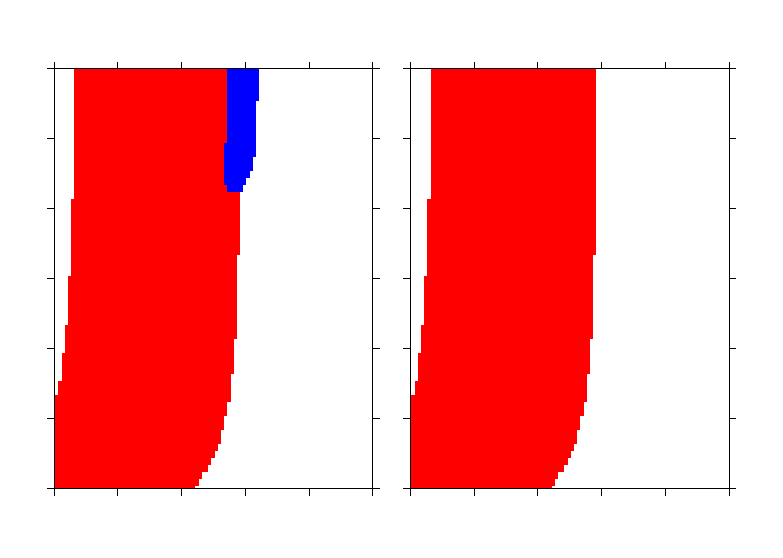
\includegraphics{Figures/Lattice.singlewire/t2nonzerophasediagrams/xifilldepend2}}%
    \gplfronttext
  \end{picture}%
\endgroup

\caption{Topological phase diagrams for $t_2 = 0.63t_1$ as a function of the filling fraction $n = N_F/N$ and coherence length $\xi$. In white: $\nu = 0$, in red: $\nu = 1$, in blue: $\nu = 2$. To the left: (anomalous) result of searching for $\Delta_k\propto \sin(2kd)$-like solutions. To the right: (normal) result of searching for $\Delta_k \propto \sin(kd)$-like solutions. Other parameters: $G = 4$, $N = 100$. }
\label{fig.phasediagram.t20.63}
\end{center}
\end{figure}

In this section the program is very similar to the above. Now however, we include the next-nearest neighbour hopping, i.e. $t_2 \neq 0$. We produce two sets of phase diagrams, one for $t_2 = t_1$ and one for $t_2 = 0.63t_1$. For these two values of $t_2$ we do the following. First we search for the same solution as in the above, i.e. the start guess is $\Delta_k \propto \sin(kd)$. This produces the diagrams to the right in figures \ref{fig.phasediagram.t21.0} and \ref{fig.phasediagram.t20.63}. Next we search for a solutions with $\sin(2kd)$-like behaviour. This results in the diagrams to the left. The topological invariant is calculated according to equation \eqref{eq.topologicalinvariant}. We go into more detail with this below. The interesting part of the figures are the blue areas. These show, where it is possible to find a self-consistent solution with a topological invariant $\nu = 2$. It is exactly this sort of solution we are after!  

In figure \ref{fig.Deltaexamples.t21.0} we go into more detail with the pairing at the points $(i)$ and $(ii)$ specified in figure \ref{fig.phasediagram.t21.0}. Remember, that the topological invariant depends on both the kinetic energy, $\varepsilon_k$, and the pairing, $\Delta_k$. Every zero of $\varepsilon_k$ for $k > 0$ contributes the sign of the pairing times the sign of the slope of $\varepsilon_k$:
\begin{equation}
\nu = \left| \text{sgn}\left(\Delta_{k_1}\partial_k\varepsilon_{k = k_1}\right) + \text{sgn}\left(\Delta_{k_1}\partial_k\varepsilon_{k = k_2}\right)\right|, \nonumber
\end{equation}
where $k_1 > 0$ and $k_2 > 0$ denote the two positive zeroes.\footnote{We could also use the negative zeroes. In both cases we can only take the zeroes of the same sign.} Now at $(i)$ we only find one solution for the pairing, irrespective of the initial guess. This single solution is $\sin(kd)$-like in that it only crosses zero at $k = 0$. There is only one positive zero of $\varepsilon_k$, so the invariant is $\nu = 1$. This behaviour is not general for the entire red region of topological invariant $\nu = 1$. Closer to the point $(ii)$, but still in the red region, we indeed find $\sin(2kd)$-like solutions. These however still have $\nu = 1$, because the filling fraction is too low to make an additional pair of zeroes of $\varepsilon_k$. At $(ii)$ we find two solutions for the pairing. Here both a (normal) $\sin(kd)$- and an (anomalous) $\sin(2kd)$-like solution are self-consistent. Since $\varepsilon_k$ now has two pairs of zeroes, the topological invariant is $\nu = 0$ and $\nu = 2$ for the normal and anomalous pairing respectively. This is because the pairing must change sign in-between the zeroes of $\varepsilon_k$ to produce a $\nu = 2$ phase as evident from the above equation and the discussion in the end of chapter \ref{Chapter12}. 

\begin{figure}
\begin{center}
% GNUPLOT: LaTeX picture with Postscript
\begingroup
  \makeatletter
  \providecommand\color[2][]{%
    \GenericError{(gnuplot) \space\space\space\@spaces}{%
      Package color not loaded in conjunction with
      terminal option `colourtext'%
    }{See the gnuplot documentation for explanation.%
    }{Either use 'blacktext' in gnuplot or load the package
      color.sty in LaTeX.}%
    \renewcommand\color[2][]{}%
  }%
  \providecommand\includegraphics[2][]{%
    \GenericError{(gnuplot) \space\space\space\@spaces}{%
      Package graphicx or graphics not loaded%
    }{See the gnuplot documentation for explanation.%
    }{The gnuplot epslatex terminal needs graphicx.sty or graphics.sty.}%
    \renewcommand\includegraphics[2][]{}%
  }%
  \providecommand\rotatebox[2]{#2}%
  \@ifundefined{ifGPcolor}{%
    \newif\ifGPcolor
    \GPcolorfalse
  }{}%
  \@ifundefined{ifGPblacktext}{%
    \newif\ifGPblacktext
    \GPblacktexttrue
  }{}%
  % define a \g@addto@macro without @ in the name:
  \let\gplgaddtomacro\g@addto@macro
  % define empty templates for all commands taking text:
  \gdef\gplbacktext{}%
  \gdef\gplfronttext{}%
  \makeatother
  \ifGPblacktext
    % no textcolor at all
    \def\colorrgb#1{}%
    \def\colorgray#1{}%
  \else
    % gray or color?
    \ifGPcolor
      \def\colorrgb#1{\color[rgb]{#1}}%
      \def\colorgray#1{\color[gray]{#1}}%
      \expandafter\def\csname LTw\endcsname{\color{white}}%
      \expandafter\def\csname LTb\endcsname{\color{black}}%
      \expandafter\def\csname LTa\endcsname{\color{black}}%
      \expandafter\def\csname LT0\endcsname{\color[rgb]{1,0,0}}%
      \expandafter\def\csname LT1\endcsname{\color[rgb]{0,1,0}}%
      \expandafter\def\csname LT2\endcsname{\color[rgb]{0,0,1}}%
      \expandafter\def\csname LT3\endcsname{\color[rgb]{1,0,1}}%
      \expandafter\def\csname LT4\endcsname{\color[rgb]{0,1,1}}%
      \expandafter\def\csname LT5\endcsname{\color[rgb]{1,1,0}}%
      \expandafter\def\csname LT6\endcsname{\color[rgb]{0,0,0}}%
      \expandafter\def\csname LT7\endcsname{\color[rgb]{1,0.3,0}}%
      \expandafter\def\csname LT8\endcsname{\color[rgb]{0.5,0.5,0.5}}%
    \else
      % gray
      \def\colorrgb#1{\color{black}}%
      \def\colorgray#1{\color[gray]{#1}}%
      \expandafter\def\csname LTw\endcsname{\color{white}}%
      \expandafter\def\csname LTb\endcsname{\color{black}}%
      \expandafter\def\csname LTa\endcsname{\color{black}}%
      \expandafter\def\csname LT0\endcsname{\color{black}}%
      \expandafter\def\csname LT1\endcsname{\color{black}}%
      \expandafter\def\csname LT2\endcsname{\color{black}}%
      \expandafter\def\csname LT3\endcsname{\color{black}}%
      \expandafter\def\csname LT4\endcsname{\color{black}}%
      \expandafter\def\csname LT5\endcsname{\color{black}}%
      \expandafter\def\csname LT6\endcsname{\color{black}}%
      \expandafter\def\csname LT7\endcsname{\color{black}}%
      \expandafter\def\csname LT8\endcsname{\color{black}}%
    \fi
  \fi
    \setlength{\unitlength}{0.0500bp}%
    \ifx\gptboxheight\undefined%
      \newlength{\gptboxheight}%
      \newlength{\gptboxwidth}%
      \newsavebox{\gptboxtext}%
    \fi%
    \setlength{\fboxrule}{0.5pt}%
    \setlength{\fboxsep}{1pt}%
\begin{picture}(7200.00,5040.00)%
    \gplgaddtomacro\gplbacktext{%
      \csname LTb\endcsname%
      \put(165,869){\makebox(0,0)[r]{\strut{}$-2$}}%
      \csname LTb\endcsname%
      \put(165,1600){\makebox(0,0)[r]{\strut{}$-1$}}%
      \csname LTb\endcsname%
      \put(165,2331){\makebox(0,0)[r]{\strut{}$0$}}%
      \csname LTb\endcsname%
      \put(165,3061){\makebox(0,0)[r]{\strut{}$1$}}%
      \csname LTb\endcsname%
      \put(165,3792){\makebox(0,0)[r]{\strut{}$2$}}%
      \csname LTb\endcsname%
      \put(429,221){\makebox(0,0){\strut{}$-3$}}%
      \csname LTb\endcsname%
      \put(916,221){\makebox(0,0){\strut{}$-2$}}%
      \csname LTb\endcsname%
      \put(1403,221){\makebox(0,0){\strut{}$-1$}}%
      \csname LTb\endcsname%
      \put(1890,221){\makebox(0,0){\strut{}$0$}}%
      \csname LTb\endcsname%
      \put(2376,221){\makebox(0,0){\strut{}$1$}}%
      \csname LTb\endcsname%
      \put(2863,221){\makebox(0,0){\strut{}$2$}}%
      \csname LTb\endcsname%
      \put(3350,221){\makebox(0,0){\strut{}$3$}}%
    }%
    \gplgaddtomacro\gplfronttext{%
      \csname LTb\endcsname%
      \put(-341,2330){\rotatebox{-270}{\makebox(0,0){\strut{}$2\Delta_k, \varepsilon_k$}}}%
      \put(1889,-109){\makebox(0,0){\strut{}$kd$}}%
      \put(429,4550){\makebox(0,0){\strut{}$(i)$}}%
      \csname LTb\endcsname%
      \put(670,4867){\makebox(0,0)[l]{\strut{}$\Delta_k/t_1 \sim \sin(1kd)$}}%
      \csname LTb\endcsname%
      \put(670,4647){\makebox(0,0)[l]{\strut{}$\varepsilon_k / t_1$}}%
    }%
    \gplgaddtomacro\gplbacktext{%
      \csname LTb\endcsname%
      \put(3584,869){\makebox(0,0)[r]{\strut{} }}%
      \csname LTb\endcsname%
      \put(3584,1600){\makebox(0,0)[r]{\strut{} }}%
      \csname LTb\endcsname%
      \put(3584,2331){\makebox(0,0)[r]{\strut{} }}%
      \csname LTb\endcsname%
      \put(3584,3061){\makebox(0,0)[r]{\strut{} }}%
      \csname LTb\endcsname%
      \put(3584,3792){\makebox(0,0)[r]{\strut{} }}%
      \csname LTb\endcsname%
      \put(3848,221){\makebox(0,0){\strut{}$-3$}}%
      \csname LTb\endcsname%
      \put(4335,221){\makebox(0,0){\strut{}$-2$}}%
      \csname LTb\endcsname%
      \put(4822,221){\makebox(0,0){\strut{}$-1$}}%
      \csname LTb\endcsname%
      \put(5309,221){\makebox(0,0){\strut{}$0$}}%
      \csname LTb\endcsname%
      \put(5796,221){\makebox(0,0){\strut{}$1$}}%
      \csname LTb\endcsname%
      \put(6283,221){\makebox(0,0){\strut{}$2$}}%
      \csname LTb\endcsname%
      \put(6770,221){\makebox(0,0){\strut{}$3$}}%
    }%
    \gplgaddtomacro\gplfronttext{%
      \csname LTb\endcsname%
      \put(5309,-109){\makebox(0,0){\strut{}$kd$}}%
      \put(3848,4550){\makebox(0,0){\strut{}$(ii)$}}%
      \csname LTb\endcsname%
      \put(4089,4867){\makebox(0,0)[l]{\strut{}$\Delta_k/t_1 \sim \sin(1kd)$}}%
      \csname LTb\endcsname%
      \put(4089,4647){\makebox(0,0)[l]{\strut{}$\Delta_k/t_1 \sim \sin(2kd)$}}%
      \csname LTb\endcsname%
      \put(4089,4427){\makebox(0,0)[l]{\strut{}$\varepsilon_k / t_1$}}%
    }%
    \gplbacktext
    \put(0,0){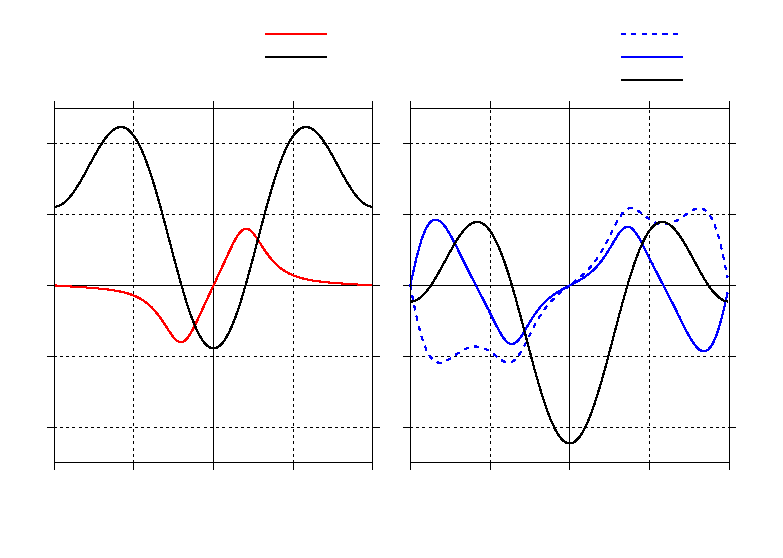
\includegraphics{Figures/Lattice.singlewire/Deltaexamples/kdepend}}%
    \gplfronttext
  \end{picture}%
\endgroup

\caption{The pairing, $\Delta_k$, and kinetic energy, $\varepsilon_k$, across the Brillouin zone. In black: $\varepsilon_k$. $(i)$, red solid line: only one solution for $\Delta_k$. This is $\sin(kd)$-like. Topological invariant: $\nu = 1$. $(ii)$, blue lines: two solutions for $\Delta_k$. Dashed blue line: $\sin(kd)$-like solution with $\nu = 0$. Solid blue line: $\sin(2kd)$-like solution with $\nu = 2$. Notice that the pairing is maximal around the zeroes of $\varepsilon_k$. Parameters: $G = 4$, $N = 100$, $\xi / d = 5$. $(i)$: $n = 0.2$, $(ii)$: $n = 0.5$.}
\label{fig.Deltaexamples.t21.0}
\end{center}
\end{figure}

The occurrence of the anomalous $\nu = 2$ phase is at high filling and high coherence lengths. The former condition we already discussed above. We must have a high filling fraction to produce two pairs of zero points of $\varepsilon_k$. The latter condition we can understand by transforming the pairing to real space. The relevant term in the Hamiltonian has the form $\sum_k \Delta_k c_{-k}c_{k}$. Plugging in $c_k = \frac{1}{\sqrt{N}}\sum_j \text{e}^{-ikx_j}x_j$, with $x_j = jd$ we get:
\begin{equation}
\sum_k \Delta_k c_{-k}c_{k} = \sum_{j,l} \tilde{\Delta}_{j,l}c_jc_l, \hspace{0.5cm} \tilde{\Delta}_{j,l} = \frac{1}{N}\sum_k\Delta_k\text{e}^{ik(x_j-x_l)}. \nonumber
\end{equation}
Hence, the real space pairing is quite simply the Fourier transform of the momentum space pairing. We use the orthogonality of $\sin(lkd)$ for different $l$ to get the following. For $\Delta_k = \Delta_1\sin(kd)$ we get $\tilde{\Delta}_{0,1} = -\tilde{\Delta}_{1,0} = -i\frac{\Delta_1}{2}$ with all others zero. In the same manner for $\Delta_k = \Delta_2\sin(2kd)$ we get $\tilde{\Delta}_{0,2} = -\tilde{\Delta}_{2,0} = -i\frac{\Delta_2}{2}$ with all others zero. Spelled out this means, that a $\sin(kd)$-like pairing has dominant \textit{nearest} neighbour pairing, whereas a $\sin(2kd)$-like pairing has dominant \text{next-nearest} neighbour pairing. This explains, why we must go to long coherence lengths. We simply need a long-range interaction for the particles to dominantly be able to pair with next-nearest neighbours. In turn a $\sin(2kd)$-like pairing in momentum space forms and the $\nu = 2$ phase is realized if the filling fraction is large as well, as discussed above. 

Now we can also explain, why the $\nu = 2$ phase region is larger for an increase in $t_2$ as illustrated by the diagrams to the left in figures \ref{fig.phasediagram.t21.0} and \ref{fig.phasediagram.t20.63}. The above analysis shows, that we need a window of two zeroes of the kinetic energy, $\varepsilon_k$. This window is simply larger for increasing $t_2$, since the kinetic energy then bends down more significantly at the Brillouin zone boundary. As $t_2$ decreases, this window narrows, and we observe that the $\nu = 2$ phase completely vanishes. 

The last important feature to study is the total free energy of the system for the different solutions, since the one with minimal free energy will be favourable for the system. The grand energy, $E_0$, is calculated in the same manner as for the double wire using:
\begin{equation}
E_0 = \frac{1}{2}\sum_k \left[\varepsilon_k - E_{F,k} - \Delta_k\braket{c^\dagger_{k}c^\dagger_{-k}}\right] = \frac{1}{2}\sum_k \left[\varepsilon_k - E_{F,k} - \frac{1}{2}|\Delta_k|^2\right], \hspace{0.5cm} T = 0
\label{eq.groundstategrandenergy.sumformula}
\end{equation}
where we use, that $\braket{c_{-k}c_k} = \frac{\Delta_k}{2E_{F,k}}$ for $T = 0$. The free energy is hereby $F = E_0 + \mu N_F$. Since we fix the filling fraction and in turn the number of fermions, it is the free energy, that must be minimal.\footnote{See section \ref{sec.2wiresgrandHFF} for an elaborate argument.}  It would be highly interesting, if the $\nu = 2$ phase could be energetically favourable in some parameter region. We therefore plot the relative difference $(F_2 - F_1)/|F_1|$, where $F_l$ is the free energy when we search for a solution of the form $\Delta_k \sim \sin(lkd)$. Hence, $F_1$ and $F_2$ correspond to the diagrams on the right and left in figure \ref{fig.phasediagram.t21.0} respectively. The result of this analysis for $t_2 = t_1$ is given in figure \ref{fig.energydifference.t21.0}. This explicitly shows, that the $\nu = 2$ phase is \textit{not} energetically favourable. Further, we notice that the higher the filling, the larger the relative difference. However, the figure also shows, that this difference is within $6\%$. This makes it plausible, that one can make the $\nu = 2$ phase favourable through some perturbation of the system. 

The figure has the additional advantage, that it shows us exactly in what region, we find $\Delta_k \sim \sin(2kd)$ solutions. Comparing this with figure \ref{fig.phasediagram.t21.0} we see, that there is a region of the $\nu = 1$ phase, where we find $\sin(2kd)$-like solutions as mentioned above. 

\begin{figure}
\begin{center}
% GNUPLOT: LaTeX picture with Postscript
\begingroup
  \makeatletter
  \providecommand\color[2][]{%
    \GenericError{(gnuplot) \space\space\space\@spaces}{%
      Package color not loaded in conjunction with
      terminal option `colourtext'%
    }{See the gnuplot documentation for explanation.%
    }{Either use 'blacktext' in gnuplot or load the package
      color.sty in LaTeX.}%
    \renewcommand\color[2][]{}%
  }%
  \providecommand\includegraphics[2][]{%
    \GenericError{(gnuplot) \space\space\space\@spaces}{%
      Package graphicx or graphics not loaded%
    }{See the gnuplot documentation for explanation.%
    }{The gnuplot epslatex terminal needs graphicx.sty or graphics.sty.}%
    \renewcommand\includegraphics[2][]{}%
  }%
  \providecommand\rotatebox[2]{#2}%
  \@ifundefined{ifGPcolor}{%
    \newif\ifGPcolor
    \GPcolorfalse
  }{}%
  \@ifundefined{ifGPblacktext}{%
    \newif\ifGPblacktext
    \GPblacktexttrue
  }{}%
  % define a \g@addto@macro without @ in the name:
  \let\gplgaddtomacro\g@addto@macro
  % define empty templates for all commands taking text:
  \gdef\gplbacktext{}%
  \gdef\gplfronttext{}%
  \makeatother
  \ifGPblacktext
    % no textcolor at all
    \def\colorrgb#1{}%
    \def\colorgray#1{}%
  \else
    % gray or color?
    \ifGPcolor
      \def\colorrgb#1{\color[rgb]{#1}}%
      \def\colorgray#1{\color[gray]{#1}}%
      \expandafter\def\csname LTw\endcsname{\color{white}}%
      \expandafter\def\csname LTb\endcsname{\color{black}}%
      \expandafter\def\csname LTa\endcsname{\color{black}}%
      \expandafter\def\csname LT0\endcsname{\color[rgb]{1,0,0}}%
      \expandafter\def\csname LT1\endcsname{\color[rgb]{0,1,0}}%
      \expandafter\def\csname LT2\endcsname{\color[rgb]{0,0,1}}%
      \expandafter\def\csname LT3\endcsname{\color[rgb]{1,0,1}}%
      \expandafter\def\csname LT4\endcsname{\color[rgb]{0,1,1}}%
      \expandafter\def\csname LT5\endcsname{\color[rgb]{1,1,0}}%
      \expandafter\def\csname LT6\endcsname{\color[rgb]{0,0,0}}%
      \expandafter\def\csname LT7\endcsname{\color[rgb]{1,0.3,0}}%
      \expandafter\def\csname LT8\endcsname{\color[rgb]{0.5,0.5,0.5}}%
    \else
      % gray
      \def\colorrgb#1{\color{black}}%
      \def\colorgray#1{\color[gray]{#1}}%
      \expandafter\def\csname LTw\endcsname{\color{white}}%
      \expandafter\def\csname LTb\endcsname{\color{black}}%
      \expandafter\def\csname LTa\endcsname{\color{black}}%
      \expandafter\def\csname LT0\endcsname{\color{black}}%
      \expandafter\def\csname LT1\endcsname{\color{black}}%
      \expandafter\def\csname LT2\endcsname{\color{black}}%
      \expandafter\def\csname LT3\endcsname{\color{black}}%
      \expandafter\def\csname LT4\endcsname{\color{black}}%
      \expandafter\def\csname LT5\endcsname{\color{black}}%
      \expandafter\def\csname LT6\endcsname{\color{black}}%
      \expandafter\def\csname LT7\endcsname{\color{black}}%
      \expandafter\def\csname LT8\endcsname{\color{black}}%
    \fi
  \fi
    \setlength{\unitlength}{0.0500bp}%
    \ifx\gptboxheight\undefined%
      \newlength{\gptboxheight}%
      \newlength{\gptboxwidth}%
      \newsavebox{\gptboxtext}%
    \fi%
    \setlength{\fboxrule}{0.5pt}%
    \setlength{\fboxsep}{1pt}%
\begin{picture}(7200.00,5040.00)%
    \gplgaddtomacro\gplbacktext{%
      \csname LTb\endcsname%
      \put(550,767){\makebox(0,0)[r]{\strut{}$1$}}%
      \csname LTb\endcsname%
      \put(550,1469){\makebox(0,0)[r]{\strut{}$2$}}%
      \csname LTb\endcsname%
      \put(550,2170){\makebox(0,0)[r]{\strut{}$3$}}%
      \csname LTb\endcsname%
      \put(550,2872){\makebox(0,0)[r]{\strut{}$4$}}%
      \csname LTb\endcsname%
      \put(550,3573){\makebox(0,0)[r]{\strut{}$5$}}%
      \csname LTb\endcsname%
      \put(550,4275){\makebox(0,0)[r]{\strut{}$6$}}%
      \csname LTb\endcsname%
      \put(550,4976){\makebox(0,0)[r]{\strut{}$7$}}%
      \csname LTb\endcsname%
      \put(745,484){\makebox(0,0){\strut{}$0$}}%
      \csname LTb\endcsname%
      \put(1741,484){\makebox(0,0){\strut{}$0.2$}}%
      \csname LTb\endcsname%
      \put(2737,484){\makebox(0,0){\strut{}$0.4$}}%
      \csname LTb\endcsname%
      \put(3733,484){\makebox(0,0){\strut{}$0.6$}}%
      \csname LTb\endcsname%
      \put(4729,484){\makebox(0,0){\strut{}$0.8$}}%
      \csname LTb\endcsname%
      \put(5725,484){\makebox(0,0){\strut{}$1$}}%
    }%
    \gplgaddtomacro\gplfronttext{%
      \csname LTb\endcsname%
      \put(176,2871){\rotatebox{-270}{\makebox(0,0){\strut{}$xi / d$}}}%
      \put(3235,154){\makebox(0,0){\strut{}$n$}}%
      \csname LTb\endcsname%
      \put(6483,767){\makebox(0,0)[l]{\strut{}$-0.015$}}%
      \put(6483,1293){\makebox(0,0)[l]{\strut{}$-0.01$}}%
      \put(6483,1819){\makebox(0,0)[l]{\strut{}$-0.005$}}%
      \put(6483,2345){\makebox(0,0)[l]{\strut{}$0$}}%
      \put(6483,2871){\makebox(0,0)[l]{\strut{}$0.005$}}%
      \put(6483,3397){\makebox(0,0)[l]{\strut{}$0.01$}}%
      \put(6483,3923){\makebox(0,0)[l]{\strut{}$0.015$}}%
      \put(6483,4449){\makebox(0,0)[l]{\strut{}$0.02$}}%
      \put(6483,4976){\makebox(0,0)[l]{\strut{}$0.025$}}%
    }%
    \gplbacktext
    \put(0,0){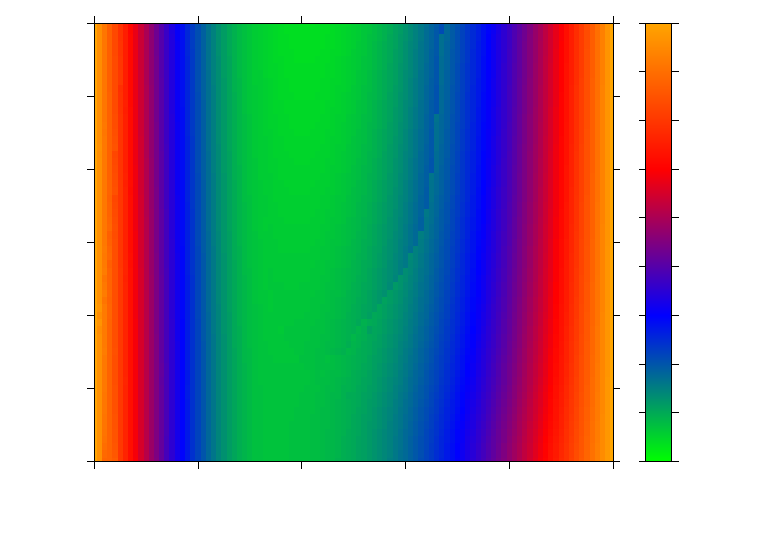
\includegraphics{E0depend}}%
    \gplfronttext
  \end{picture}%
\endgroup

\caption{Relative free energy difference $(F_2 - F_1) / |F_1|$ of searching for $\Delta_k \sim \sin(2kd)$ and $\Delta_k\sim \sin(kd)$ corresponding to the diagrams in figure \ref{fig.phasediagram.t21.0}. A positive value indicates, that the $\sin(kd)$-like solution is energetically favourable. Parameters: $t_2 = t_1$, $G = 4$, $N = 100$. }
\label{fig.energydifference.t21.0}
\end{center}
\end{figure}


\part{Discussions and Conclusions}
\newpage 

\chapter{Discussion} 

\label{Chapter14} 
\lhead{Part V. \emph{Discussions \& Conclusions}}
\chead{Chapter 14. \emph{Discussion}} % Change X to a consecutive number; this is for the header on each page - perhaps a shortened title

\section{Cross over in the double wire system and physical discrepancies} \label{sec.Discussion.2wires.crossover}
To have a full understanding of the cross over in the double wire system, we had to use both a bulk and boundary perspective. The bulk effect for the separated wires is, that there is only a topologically nontrivial intrawire $p$-wave pairing present. The resulting boundary effect is, that Majorana edge states can form with no energy cost. Oppositely when the wires are very close, only a topologically trivial interwire $s$-wave pairing is present. In turn there are no edge states. 

To understand the transition in-between this bulk-boundary correspondence is even more important. As the wires are brought closer together, the interwire interaction respects a time reversal symmetry with $T^2 = - \mathbb{I}$. As the analytical analysis of chapter \ref{Chapter10} shows, the edge states are time reversal (Kramers) partners. Therefore, the edge states are unaffected by the interwire interaction. This holds until a mean field is chosen, namely the interwire $s$-wave pairing. This interwire pairing can do two things through a specific choice of its phase: it can respect the $T^2 = - \mathbb{I}$ symmetry or not. If it respects the symmetry, the edge states are still uncoupled. A calculation of the bulk topological invariant shows, that this holds until the energy gap closes. Then the bulk is topologically trivial and no edge states are present. If it \textit{breaks} this symmetry, the edge states are no longer uncoupled. Actually they gain a nonzero energy for any nonzero interwire pairing. In turn the bulk energy gap does not have to close for the edge state to vanish. 

The nontrivial result of the numerical analysis is, that the interwire pairing chooses to break the $T^2 = -\mathbb{I}$ symmetry. This is simply because it is the energetically favourable choice. Further, a coexistence of the $p$-wave and $s$-wave pairing is observed in the transition. 

This mean field result does however have an important physical discrepancy. Consider the gap equations for the double wire system, equation \eqref{eq.2wiresgapequations}. As we bring the wires closer together the intrawire pairing is not affected by the interwire induced interaction until an interwire pairing forms. This is absurd. The interwire interaction will of course alter the physical properties internally in each wire, also when the wires are far apart. This also leads to the odd prediction, that the critical temperature for intrawire pairing is unaffected by the interwire interaction, as long as the interwire pairing is absent. This is \textit{not} physically reasonable. 

The reason for this discrepancy is the same as the reason why, the mean field approximation breaks down for a single wire above the critical temperature. When no mean field is present, the mean field approximation is the same as neglecting the interaction all together. There is however a way to (partially) remedy this using the socalled self-energy. The self-energy is the energy shift a fermion experiences due to its interaction with all the others. It is clear, that this self-energy will increase as the wires are brought closer together. 

\section{Kitaev chain} \label{sec.Discussion.KitaevChain}
In this thesis we have studied fermionic one-dimensional \textit{gasses}. The original work of Kitaev is based on fermions sitting in a one-dimensional \textit{lattice} with nearest neighbour hopping and pairing \cite{KitaevQuantumWires}. In recent work by Alecce and Dell'Anna an extended version of the Kitaev chain with $r$ neighbours is considered \cite{Alecce.extendKitaev}. They find, that if the hopping and pairing decays sufficiently slow, topological phases with up to $r$ Majorana edge states can be found, hence exceeding the Kitaev result of a single Majorana edge state. 

In this connection we have briefly studied, whether this is possible in our 1D-3D Fermi-Bose mixture. More specifically we think of the fermions as sitting in an optical lattice with nearest and next-nearest neighbour hopping. We must then self-consistently solve for the pairing, $\Delta_k$, and compute the $\mathbb{Z}$-topological invariant $\nu = 2\text{CS}_1$. Since we consider two neighbours, we search for $\nu = \pm 2$. Unfortunately, we have not been able to find such a solution. We speculate, that the reason for this is, that the Yukawa interaction is simply not long range enough. This is supported by the fact, that we can find $\nu = \pm 2$ solutions, when the interaction drops of as $|x|^{-\alpha}$, with $\alpha < 1$. This is also consistent with the findings of Alecce and Dell'Anna. Specifically, they show that the hopping and pairing both have to decay with $\alpha < 1$ for the number of Majorana edge states to exceed 1. This way of producing several edge states systems in the Fermi-Bose mixture framework is therefore considered inapplicable. 



\chapter{Conclusion} 
\label{Chapter15} 
\lhead{Part V. \emph{Discussions \& Conclusions}}
\chead{Chapter 15. \emph{Conclusion}} 

We have studied the many-body effects of wires of identical fermions embedded in a three-dimensional Bose-Einstein condensate. We have shown, that a point interaction between the fermions and bosons lead to an induced attractive interaction between the fermions of the Yukawa form in the weak-coupling limit. In a mean field approach we have shown, that the single wire system realises the Kitaev model of superfluidity. In turn we have found selfconsistent numerical solutions for the pairing and chemical potentials, that demonstrates a superfluid phase with $p$-wave pairing. Using the linearized gap equation we have numerically demonstrated, that any nonzero point interaction between the fermions and bosons lead to the formation of the superfluid. We have calculated the bulk topological invariant of the system and demonstrated, that the ground state is topologically nontrivial. This is verified explicitly by finding an approximate solution for the resulting edge states at the boundary of the wire. 

For the double wire system the above steps have been repeated. Here the interwire interaction is shown to lead to a competing interwire $s$-wave pairing. The resulting Hamiltonian has the structure of a spin-$1/2$ system with $p$-wave pairing between identical spins and $s$-wave pairing between opposite spins. The competition between the pairings is shown to be controllable through the interwire distance or analogously the Bose-Einstein coherence length. The edge states in each wire in the separated wire system are shown to be Kramers partners in accordance with a time reversal symmetry, that squares to minus the identity. By calculating the topological invariant we show, that there are two possible and physically distinct configurations of the system. These configurations are different only in the phase of the interwire pairing. In one, as the wires are brought closer together, the interwire pairing chooses a phase, that obeys the time reversal symmetry. In turn a topological phase transition, where the bulk energy gap closes, must occur as the wires are brought closer together. In the other, the interwire pairing chooses a phase, that breaks this time reversal symmetry. The Kramers partners of edge states are then shown to couple and gain a nonzero energy. Then in a numerical analysis we find the selfconsistent solutions for the pairing and chemical potentials. We hereby show, that the configuration that breaks the time reversal symmetry is the energetically favourable. Using mean field theory, we therefore predict, that the two wire system will undergo a normal, nontopological phase transition between a topologically nontrivial and trivial phase. This is the main result of the thesis.

We emphasize, that we are aware, that the mean field approach is problematic for these one-dimensional systems. However, we speculate that in the long coherence length limit, the results will be qualitatively correct. 

%----------------------------------------------------------------------------------------
%	THESIS CONTENT - APPENDICES
%----------------------------------------------------------------------------------------

\addtocontents{toc}{\vspace{2em}} % Add a gap in the Contents, for aesthetics

\appendix % Cue to tell LaTeX that the following 'chapters' are Appendices

% Include the appendices of the thesis as separate files from the Appendices folder
% Uncomment the lines as you write the Appendices

\input{Appendices/AppendixA}
% Appendix B

\chapter{General real space induced interaction} % Main appendix title

\label{Appendix.inducedinteraction.realspace} % For referencing this appendix elsewhere, use \ref{AppendixC}
\chead{}
\lhead{Appendix B. \emph{General real space induced interaction}} % This is for the header on each page - perhaps a shortened title
In this appendix we calculate the real space induced interaction in the weak coupling limit for general Matsubara frequency $\omega_m = 2\pi m k_B T$. This is only done for $l_t = 0$. 

From equation \eqref{eq.VFFindXBEC} we have the induced interaction in momentum space for all $l_t > 0$:
\begin{equation}
V_{\text{ind}}(q, i\omega_m) = g_{BF}^2\int\frac{d^2k_\perp}{(2\pi)^2}\; \chi_\text{BEC}(q, \mathbf{k}_\perp, i\omega_m)\text{e}^{-\frac{l_t^2}{2}k_\perp^2},\nonumber
\end{equation}
with $\chi_\text{BEC}(\mathbf{k}, i\omega_m) = -\frac{k^2}{m_B}\frac{n_B}{\omega^2_m + E_{B,k}^2}$ the BEC density-density correlation function, and $E^2_{B,k} = \frac{k^2}{2m_B}\left(\frac{k^2}{2m_B} + 2n_Bg_B\right)$ the Bogoliubov BEC spectrum. The real space induced interaction is the Fourier transform of the above. Therefore, we can use the following limiting procedure for $l_t = 0$:
\begin{equation}
\tilde{V}_{\text{ind}}(x, i\omega_m) = \lim_{d \to 0}\left[g_{BF}^2\int\frac{d^3k}{(2\pi)^3}\; \chi_\text{BEC}(\mathbf{k}, i\omega_m)\text{e}^{i\mathbf{k}\cdot \mathbf{r}_d}\right] = \lim_{d \to 0} I(\mathbf{r}_d, \omega_m), 
\label{eq.limitVindxomegam}
\end{equation}
which defines $I(\mathbf{r}, \omega_m)$ and where $\mathbf{r}_d = (x, \mathbf{d})$. With a bit of rearranging we get the expression:
\begin{equation}
I(\mathbf{r}, \omega_m) = +4m_Bg^2_{BF}n_B\int \frac{d^3k}{(2\pi)^3} \frac{k^2}{g(k)}\text{e}^{i\mathbf{k}\cdot\mathbf{r}} = +4m_Bg^2_{BF}n_B\int_0^\pi d\theta \sin(\theta)\int_0^{\infty} \frac{dk}{(2\pi)^2} \frac{k^4}{g(k)}\text{e}^{ikr\cos(\theta)}, \nonumber
\end{equation}
where we define $g(k) = 4m_B^2\omega^2_m + k^2(k^2 + 2/\xi^2)$, and where $1/\xi^2 = 2m_Bn_Bg_B$ defines the BEC coherence length $\xi$. Here we let $\theta$ be the angle between $\mathbf{k}$ and $\mathbf{r}$ and use, that the integrand does not depend on the azimuthal angle $\phi$. Performing the $\theta$ integral directly we get:
\begin{equation}
I(\mathbf{r}, \omega_m) = -\frac{2m_Bg^2_{BF}n_B}{\pi}\int \frac{dk}{2\pi i} \frac{k^3}{g(k)}\text{e}^{ikr}, \nonumber
\end{equation}
where the limits are implicitly $\pm \infty$. We will now think of $k$ as a complex variable and make a half-circle contour $\mathcal{C}$ in the upper half-plane. Since the integrand goes exponentially fast to zero on the boundary of $\mathcal{C}$, we get:
\begin{equation}
I(\mathbf{r}, \omega_m) = -\frac{2m_Bg^2_{BF}n_B}{\pi}\int_{\mathcal{C}} \frac{dk}{2\pi i} \frac{k^3}{g(k)}\text{e}^{ikr}, \nonumber
\end{equation}
in the limit of infinite radius $R$ of the half-circle. By Cauchy's residue theorem we can then calculate the integral by calculating the residues of the integrand. To do this we need the poles of $g(k)$, that $\mathcal{C}$ surrounds, hence the poles in the upper half-plane. We therefore solve $g(k) = 0$, a quadratic equation in $k^2$, with the two solutions:
\begin{equation}
k^2_{\pm} = -\frac{1}{\xi^2}\left(1 \pm \sqrt{1 - \left(\frac{\omega_m}{n_Bg_B}\right)^2}\right), \nonumber
\end{equation} 
where the square root is chosen to give positive real parts. The roots of $g(k)$ are then $ik_+, -ik_+, ik_-, -ik_-$, with $ik_{\pm}$ the roots in the upper half-plane, and with: 
\begin{equation}
k_{\pm} = \frac{1}{\xi}\sqrt{1\pm \sqrt{1 - \left(\frac{\omega_m}{n_Bg_B}\right)^2}} = \sqrt{ 2m_Bn_Bg_B\left( 1 \pm \sqrt{1 - \left(\frac{\omega_m}{n_Bg_B}\right)^2 } \right) }
\label{eq.polesVindxomegam}
\end{equation}
We can therefore write $g(k) = (k + ik_+)(k - ik_-)(k + ik_-)(k - ik_-)$ and the residues in the upper half-plane poles $ik_{\pm}$ then simply becomes:
\begin{equation}
\text{Res}(f, k_{\pm}) = \lim_{k\to ik_{\pm}} (k - ik_{\pm})f(k), \hspace{0.5cm} f(k) = \frac{k^3}{g(k)}\text{e}^{ikr}. \nonumber
\end{equation}
Now using $\int_{\mathcal{C}} \frac{dk}{2\pi i} \frac{k^3}{g(k)}\text{e}^{ikr} = \text{Res}(f, k_+) + \text{Res}(f, k_-)$ we get the expression:
\begin{equation}
I(\mathbf{r}, \omega_m) = -\frac{m_Bg^2_{BF}n_B}{2\pi r}\left[ \text{e}^{-k_+r} + \text{e}^{-k_-r} + \frac{1}{ \sqrt{1 - \left(\frac{\omega_m}{n_Bg_B}\right)^2} }\left(\text{e}^{-k_+r} - \text{e}^{-k_-r}  \right) \right]. \nonumber
\end{equation}
Finally taking the limit in equation \eqref{eq.limitVindxomegam} gives:
\begin{equation}
\tilde{V}_{\text{ind}}(x, i\omega_m) = -\frac{m_Bg^2_{BF}n_B}{2\pi |x|}\left[ \text{e}^{-k_+|x|} + \text{e}^{-k_-|x|}  + \frac{1}{ \sqrt{1 - \left(\frac{\omega_m}{n_Bg_B}\right)^2} }\left(\text{e}^{-k_+|x|} - \text{e}^{-k_-|x|}  \right) \right], 
\end{equation}
by simply replacing $r$ with $|x|$. We know, that for $\omega_m = 0$ we must get the Yukawa interaction. In this situation $k_- = 0, k_+ = \sqrt{2}/\xi$ and we get:
\begin{equation}
\tilde{V}_{\text{ind}}(x, i\omega_m = 0) = -\frac{m_Bg^2_{BF}n_B}{\pi |x|}\text{e}^{-\sqrt{2}|x|/\xi}, \nonumber
\end{equation}
which is identical to equation \eqref{eq.Vx_lt=0}. 


% Appendix C

\chapter{Quasiparticle distribution, 1 wire} % Main appendix title

\label{Appendix.distribution.quasiparticles} % For referencing this appendix elsewhere, use \ref{AppendixA}
\chead{}
\lhead{Appendix C. \emph{Quasiparticle distribution, 1 wire}} % This is for the header on each page - perhaps a shortened title
In this appendix we in detail describe how to take the thermal average for the single wire within the mean field approximation. We use this to show, that the quasiparticles are Fermi-Dirac distributed. Throughout we neglect the ground state grand energy $E_0 = \frac{1}{2}\sum_k \left[\varepsilon_k - \Delta_k \braket {c^\dagger_k c^\dagger_{-k}}\right]$.

Throughout the thesis we keep the mean number of fermions, $\braket{N_F}$, constant. However, we do not fix the number of quasiparticles ($\gamma$). This means, that the partition function takes the form of the \textit{canonical} partition function: $Z = \tr\left[\text{e}^{-\beta H_{FF}}\right]$. In terms of thermodynamics this means, that every single quasiparticle is in thermal (and not diffusive) equilibrium with all the others, hence working as a heat reservoir. Since the Hamiltonian is diagonal in the quasiparticles $\gamma_k$, we can calculate the partition function for each $k$ by replacing $H_{FF}$ with the $k$'th (diagonal) term. We then get:
\begin{equation}
Z_k = \tr\left[\text{e}^{-\beta H_{FF,k}}\right] = \tr\left[\text{e}^{-\beta E_{F,k}\gamma^\dagger_k\gamma_k }\right] = 1 + \text{e}^{-\beta E_{F,k}}. \nonumber
\end{equation}     
For the calculation of the trace, we use the single particle complete basis $\{\ket{\text{S}}_0, \gamma^\dagger_k\ket{\text{S}}_0\}$. This is all a rather involved way of saying, that the quasiparticle can either be absent, $\ket{\text{S}}_0$, and have zero energy or present, $\gamma^\dagger_k\ket{\text{S}}_0$, and have energy $E_{F,k}$. The total partition function is then simply $Z = \prod_k Z_k$. The mean number of quasiparticles with momentum $k$ is given by $\braket{\gamma^\dagger_k\gamma_k} = \tr\left[\text{e}^{-\beta H_{FF}}\gamma^\dagger_k\gamma_k\right]/Z$. For the calculation of the trace we need a complete basis. The basis consists of states with any number of quasiparticles present with all possible momenta. These states can all be written as: $\prod_{q\in K} \gamma^\dagger_q \ket{\text{S}}_0$, where $K$ is an arbitrary set of momenta. Since $\gamma^\dagger_k\gamma_k$ counts the number of quasiparticles present with momentum $k$, we only need sets $K$ with $k \in K$. For these states we get:
\begin{equation}
\text{e}^{-\beta H_{FF}} \gamma^\dagger_k \gamma_k\prod_{q\in K} \gamma^\dagger_q \ket{\text{S}}_0 = \text{e}^{-\beta H_{FF}}\prod_{q\in K} \gamma^\dagger_q \ket{\text{S}}_0  = \text{e}^{-\beta \sum_{q \in K} E_{F,q}} \prod_{q\in K} \gamma^\dagger_q \ket{\text{S}}_0. \nonumber
\end{equation}
The desired trace is then the sum of $\text{e}^{-\beta \sum_{q \in K} E_{F,q}}$ for all combinations of $K$ containing $k$:
\begin{equation}
\tr\left[\text{e}^{-\beta H_{FF}}\gamma^\dagger_k\gamma_k\right] = \sum_K \text{e}^{-\beta \sum_{q \in K} E_{F,q}} = \text{e}^{-\beta E_{F,k}}\prod_{q \neq k} \left[1 + \text{e}^{-\beta E_{F,q}}\right] = \text{e}^{-\beta E_{F,k}} \frac{Z}{Z_k}. \nonumber 
\end{equation}
The second equality is most easily verified by writing out the product. By doing this one explicitly sees, that all combinations of energies are present. Finally: 
\begin{equation}
\braket{\gamma^\dagger_k\gamma_k} = \frac{\tr\left[\text{e}^{-\beta H_{FF}}\gamma^\dagger_k\gamma_k\right]}{Z} = \frac{\text{e}^{-\beta E_{F,k}}}{Z_k} = \frac{\text{e}^{-\beta E_{F,k}}}{1 + \text{e}^{-\beta E_{F,k}}} = f(E_{F,k}),
\end{equation}
with $f(E)$ the Fermi-Dirac distribution. This is the average number of $\gamma_k$ particles in the thermalized state of the system. We emphasize that this calculation is a rather formal approach. In a simpler manner we have, that the average number of quasiparticles with momentum $k$ is given by: $\sum_n n P_k(n) = \frac{1}{Z_k}\sum_{n = 0}^{1} \text{e}^{ -n\beta E_{F,k} } = f( E_{F,k} )$, with the probability of occupation with $n$ quasiparticles in the $k$'th state given by $\text{e}^{-n\beta E_{F,k}}/Z_k$. In any regard the above explicitly shows, how we equivalently can formulate this using the second quantized operators. 

By going from the $c$ to $\gamma$ operators we can calculate all desired averages.

% Appendix D

\chapter{Quasiparticle distribution} % Main appendix title

\label{Appendix.distribution.quasiparticles} 
\chead{Appendix D. \emph{Quasiparticle distribution}}
\lhead{Part V. Appendices} 
In this appendix we calculate the distribution function for fermionic particles, that are not number-conserved. This distribution function is used for the quasiparticles of the single and double wire system. 

Let $H = \sum_i E_i a^\dagger_i a_i$ be the Hamiltonian with $a^\dagger_i$ a fermionic creation operator:
\begin{equation}
\{a_i, a^\dagger_j\} = \delta_{i,j}, 
\label{eq.appendix.fermioniccommutationrelation}
\end{equation}
and $i$ the quantum number. We assume, that the number of these fermions are \textit{not} conserved. This means, that the partition function takes the form of the \textit{canonical} partition function: $Z = \tr\left[\text{e}^{-\beta H}\right]$. In terms of thermodynamics this means, that every single fermion is in thermal (and not diffusive) equilibrium with all the others, hence working as a heat reservoir. Since the Hamiltonian is diagonal, we can calculate the partition function for each $i$ by replacing $H$ with the $i$'th (diagonal) term. We then get:
\begin{equation}
Z_i = \tr\left[\text{e}^{-\beta H_i}\right] = \tr\left[\text{e}^{-\beta E_ia^\dagger_i a_i }\right] = 1 + \text{e}^{-\beta E_i}. \nonumber
\end{equation}     
For the calculation of the trace, we use the single particle complete basis $\{\ket{0}, a^\dagger_i\ket{0}\}$, with $\ket{0}$ the ground state: $a_i\ket{0} = 0$. This is all a rather involved way of saying, that the fermion can either be absent, $\ket{0}$, and have zero energy or be present, $a^\dagger_i\ket{0}$, and have energy $E_i$. The total partition function is then simply $Z = \prod_i Z_i$. The mean number of fermions with quantum number $i$ is given by $\braket{a^\dagger_ia_i} = \tr\left[\text{e}^{-\beta H}a^\dagger_ia_i\right]/Z$. For the calculation of the trace we need a complete basis. The basis consists of states with any number of fermions present with all possible quantum numbers. These states can all be written as: $\prod_{j\in J} a^\dagger_j \ket{0}$, where $J$ is an arbitrary set of quantum numbers. Since $a^\dagger_ia_i$ counts the number of fermions present with quantum number $i$, we only need sets $J$ with $i \in J$. For these states we get:
\begin{equation}
\text{e}^{-\beta H} a^\dagger_i a_i\prod_{j\in J} a^\dagger_j \ket{0} = \text{e}^{-\beta H}\prod_{j\in J} a^\dagger_i \ket{0} = \text{e}^{-\beta \sum_{j \in J} E_j} \prod_{j \in J} a^\dagger_i \ket{0}. \nonumber
\end{equation}
The desired trace is then the sum of $\text{e}^{-\beta \sum_{j \in J} E_j}$ for all combinations of $J$ containing $i$:
\begin{equation}
\tr\left[\text{e}^{-\beta H}a^\dagger_ia_i\right] = \sum_J \text{e}^{-\beta \sum_{j \in J} E_j} = \text{e}^{-\beta E_i}\prod_{j \neq i} \left[1 + \text{e}^{-\beta E_j}\right] = \text{e}^{-\beta E_i} \frac{Z}{Z_i}. \nonumber 
\end{equation}
The second equality is most easily verified by writing out the product. By doing this one explicitly sees, that all combinations of energies are present. Finally: 
\begin{equation}
\braket{a^\dagger_ia_i} = \frac{\tr\left[\text{e}^{-\beta H}a^\dagger_ia_i\right]}{Z} = \frac{\text{e}^{-\beta E_i }}{Z_i} = \frac{\text{e}^{-\beta E_i}}{ 1 + \text{e}^{-\beta E_i} } = \frac{1}{ \text{e}^{\beta E_i} + 1 } = f(E_i),
\end{equation}
with $f(E)$ the Fermi-Dirac distribution. This is the average number of $a$ particles in the thermalized state of the system. We emphasize that this calculation is a rather formal approach. In a simpler manner we have, that the average number of fermions with quantum number $i$ is given by: $\sum_n n P_i(n) = \frac{1}{Z_i}\sum_{n = 0}^{1} \text{e}^{ -n\beta E_i } = f( E_i )$, with the probability of occupation with $n$ fermions in the $i$'th state given by $\text{e}^{-n\beta E_i}/Z_i$. In any regard the above explicitly shows, how we equivalently can formulate this using the second quantized operators. 

The present appendix hereby in detail shows, that fermionic free particles with energy $E_i$, that are not number-conserved, are distributed according to $f(E_i)$. For the single wire system we make the identification: $a_i \to \gamma_k$. For the double wire system: $a_i \to \gamma_{j,k}$, where $j$ specifies the wire and $k$ is the momentum. 

\chapter{Critical temperature, separated wires} % Main chapter title

\label{Appendix.criticaltemperature} % For referencing this appendix elsewhere, use \ref{AppendixA}
\chead{E. \emph{Critical temperature}}
\lhead{Part V. Appendices} 

%----------------------------------------------------------------------------------------
In this appendix we will first derive a linearized gap equation. See section \ref{sec.linearizedgapequation}. This will give us a more efficient way of calculating the critical temperature $T_c$ for the transition between the superfluid and normal phase. In section \ref{sec.criticaltemperature.numerical} we will then solve the equation numerically and investigate the dependency of $T_c$ on the gas parameters $(n_Ba_{BF}^3)^{1/3}$ and $(n_Ba_B^3)^{1/3}$. 

\section{Linearized gap equation} \label{sec.linearizedgapequation}
In the analysis of chapter \ref{Chapter6} the estimation of the critical temperature $T_c$ is quite tedious. We have to wait for an increasing number of iterations near $T_c$ to get a good estimate and calculating the critical temperature as a function of the parameters of the problem is out of the question. In this section we will describe a much more efficient way of estimating the critical temperature through \textit{the linearized gap equation}. 

For the separated wires, the gap equation in integral form is:
\begin{equation}
\Delta^{11}_k = - \int \frac{dk'}{2\pi} W_{\text{ind}}(k,k')\frac{\tanh\left(\frac{\beta E_{F,k}}{2}\right)}{2E_{F,k'}}\Delta^{11}_{k'}. \nonumber
\end{equation} 
As we saw in chapter \ref{Chapter6} the gap goes to zero at the critical temperature $T_c$: $\Delta^{11}_k(T_c) = 0$. The energy $E_{F,k} = \sqrt{\epsilon_k^2 + |\Delta^{11}_k|^2}$ is quadratic in the gap. It follows that by only retaining the gap to first order, we obtain a linear equation near $T_c$:
\begin{equation}
\Delta^{11}_k = - \int \frac{dk'}{2\pi} W_{\text{ind}}(k,k')\frac{\tanh\left(\frac{\beta \varepsilon_k}{2}\right)}{2\varepsilon_k} \Delta^{11}_{k'}.
\label{eq.GapequationIntegralLinear}
\end{equation} 
Here we have also used, that $\frac{\tanh\left(\frac{\beta \varepsilon_k}{2}\right)}{2\varepsilon_k}$ is even in $\varepsilon_k$, so that the absolute value from the square root can be omitted. This defines a linear equation with eigenvalue $1$: $\Delta^{11}_k = L(\Delta^{11}_k)$. $L$ is then a linear transformation defined by the integral above. Hence, the program for the evaluation of $T_c$ is now clear. We must find the highest temperature at which, there is an eigenvalue of 1. Notice, that this specifies where the normal to superfluid phase transition occures. This also means, that the chemical potential in $\varepsilon_k = \frac{k^2}{2m_F} - \mu$ can be taken to be the normal phase chemical potential (the chemical potential for the free gas). 

\section{Calculating the critical temperature} \label{sec.criticaltemperature.numerical}
In this section we will describe how in practice to perform the calculation outlined in the above. 

We need to but the linear equation on matrix form. From equation \eqref{eq.GapequationIntegralLinear} we get the matrix equation:
\begin{equation}
\Delta^{11}_k = L \Delta^{11}_k, \hspace{0.5cm} L(k,k') = -\frac{dk'}{2\pi} W_{\text{ind}}(k,k')\frac{\tanh(\beta \varepsilon_{k'}/2)}{2\varepsilon_{k'}}. 
\label{eq.Gapmatrixequation}
\end{equation}
Explicitly we define a cutoff $k_{\text{up}}$ and spacing $dk'$. We then need to make $k_{\text{up}}$ large enough and $dk'$ small enough for the eigenvalues to have converged. From the form of $L(k,k')$ it is also clear, that $L$ is not a symmetric matrix; each row of $L$ has all the possible values of $\varepsilon_{k'}$, but each column only has a single value belonging to the entire column. The evaluation is performed in MatLab in the following fashion. For a fixed set of parameters we start out with an initial guess $T$ for $T_c$, that we know is too high. We then iteratively decrease $T$ by a small amount $dT$ and calculate the largest eigenvalue for each iteration. When the largest eigenvalue becomes larger than 1, we halt the iteration and set the critical temperature to the current value of $T$. The numerical analysis is a balancing act. We have to choose a resolution fine enough, defined by $dk'$ and $k_{\text{up}}$, for the eigenvalues to have converged to the eigenvalue for the integral operator, and still keep the matrix $L$ small enough for the analysis to be feasible. In this context it is crucial that we have a closed form expression for $W_{\text{ind}}(k,k')$ in the $l_t \to 0$ limit. As already commented we use the free gas chemical potential. Since $T/T_F \ll 1$ for all relevant temperatures, we use the Sommerfeld expansion: $\frac{\mu(T)}{\epsilon_{F,0}} = 1 + \frac{\pi^2}{12}\left(\frac{T}{T_F}\right)^2$. See equation \eqref{eq.Sommerfeldexpansionchemicalpotential}. 

The aboved described strategy is made graphic in figure \ref{fig.TCeigenvalues}. For a specific set of parameters, we have calculated the five highest eigenvalues of $L$ as a function of $T$. We notice, that it is solely the largest eigenvalue, that determines the critical temperature: the eigenvalue crosses 1 for one specific temperature. In the present case: $T_c \approx 0.130 T_F$. The next 4 eigenvalues are significantly lower. 

\begin{figure} 
\begin{center}  
% GNUPLOT: LaTeX picture with Postscript
\begingroup
  \makeatletter
  \providecommand\color[2][]{%
    \GenericError{(gnuplot) \space\space\space\@spaces}{%
      Package color not loaded in conjunction with
      terminal option `colourtext'%
    }{See the gnuplot documentation for explanation.%
    }{Either use 'blacktext' in gnuplot or load the package
      color.sty in LaTeX.}%
    \renewcommand\color[2][]{}%
  }%
  \providecommand\includegraphics[2][]{%
    \GenericError{(gnuplot) \space\space\space\@spaces}{%
      Package graphicx or graphics not loaded%
    }{See the gnuplot documentation for explanation.%
    }{The gnuplot epslatex terminal needs graphicx.sty or graphics.sty.}%
    \renewcommand\includegraphics[2][]{}%
  }%
  \providecommand\rotatebox[2]{#2}%
  \@ifundefined{ifGPcolor}{%
    \newif\ifGPcolor
    \GPcolorfalse
  }{}%
  \@ifundefined{ifGPblacktext}{%
    \newif\ifGPblacktext
    \GPblacktexttrue
  }{}%
  % define a \g@addto@macro without @ in the name:
  \let\gplgaddtomacro\g@addto@macro
  % define empty templates for all commands taking text:
  \gdef\gplbacktext{}%
  \gdef\gplfronttext{}%
  \makeatother
  \ifGPblacktext
    % no textcolor at all
    \def\colorrgb#1{}%
    \def\colorgray#1{}%
  \else
    % gray or color?
    \ifGPcolor
      \def\colorrgb#1{\color[rgb]{#1}}%
      \def\colorgray#1{\color[gray]{#1}}%
      \expandafter\def\csname LTw\endcsname{\color{white}}%
      \expandafter\def\csname LTb\endcsname{\color{black}}%
      \expandafter\def\csname LTa\endcsname{\color{black}}%
      \expandafter\def\csname LT0\endcsname{\color[rgb]{1,0,0}}%
      \expandafter\def\csname LT1\endcsname{\color[rgb]{0,1,0}}%
      \expandafter\def\csname LT2\endcsname{\color[rgb]{0,0,1}}%
      \expandafter\def\csname LT3\endcsname{\color[rgb]{1,0,1}}%
      \expandafter\def\csname LT4\endcsname{\color[rgb]{0,1,1}}%
      \expandafter\def\csname LT5\endcsname{\color[rgb]{1,1,0}}%
      \expandafter\def\csname LT6\endcsname{\color[rgb]{0,0,0}}%
      \expandafter\def\csname LT7\endcsname{\color[rgb]{1,0.3,0}}%
      \expandafter\def\csname LT8\endcsname{\color[rgb]{0.5,0.5,0.5}}%
    \else
      % gray
      \def\colorrgb#1{\color{black}}%
      \def\colorgray#1{\color[gray]{#1}}%
      \expandafter\def\csname LTw\endcsname{\color{white}}%
      \expandafter\def\csname LTb\endcsname{\color{black}}%
      \expandafter\def\csname LTa\endcsname{\color{black}}%
      \expandafter\def\csname LT0\endcsname{\color{black}}%
      \expandafter\def\csname LT1\endcsname{\color{black}}%
      \expandafter\def\csname LT2\endcsname{\color{black}}%
      \expandafter\def\csname LT3\endcsname{\color{black}}%
      \expandafter\def\csname LT4\endcsname{\color{black}}%
      \expandafter\def\csname LT5\endcsname{\color{black}}%
      \expandafter\def\csname LT6\endcsname{\color{black}}%
      \expandafter\def\csname LT7\endcsname{\color{black}}%
      \expandafter\def\csname LT8\endcsname{\color{black}}%
    \fi
  \fi
    \setlength{\unitlength}{0.0500bp}%
    \ifx\gptboxheight\undefined%
      \newlength{\gptboxheight}%
      \newlength{\gptboxwidth}%
      \newsavebox{\gptboxtext}%
    \fi%
    \setlength{\fboxrule}{0.5pt}%
    \setlength{\fboxsep}{1pt}%
\begin{picture}(7200.00,5040.00)%
    \gplgaddtomacro\gplbacktext{%
      \csname LTb\endcsname%
      \put(814,767){\makebox(0,0)[r]{\strut{}$0$}}%
      \csname LTb\endcsname%
      \put(814,1819){\makebox(0,0)[r]{\strut{}$0.5$}}%
      \csname LTb\endcsname%
      \put(814,2872){\makebox(0,0)[r]{\strut{}$1$}}%
      \csname LTb\endcsname%
      \put(814,3924){\makebox(0,0)[r]{\strut{}$1.5$}}%
      \csname LTb\endcsname%
      \put(814,4976){\makebox(0,0)[r]{\strut{}$2$}}%
      \csname LTb\endcsname%
      \put(1009,484){\makebox(0,0){\strut{}$0$}}%
      \csname LTb\endcsname%
      \put(2442,484){\makebox(0,0){\strut{}$0.05$}}%
      \csname LTb\endcsname%
      \put(3875,484){\makebox(0,0){\strut{}$0.1$}}%
      \csname LTb\endcsname%
      \put(5307,484){\makebox(0,0){\strut{}$0.15$}}%
      \csname LTb\endcsname%
      \put(6740,484){\makebox(0,0){\strut{}$0.2$}}%
    }%
    \gplgaddtomacro\gplfronttext{%
      \csname LTb\endcsname%
      \put(176,2871){\rotatebox{-270}{\makebox(0,0){\strut{}$Eigenvalue$}}}%
      \put(3874,154){\makebox(0,0){\strut{}$T/T_F$}}%
    }%
    \gplbacktext
    \put(0,0){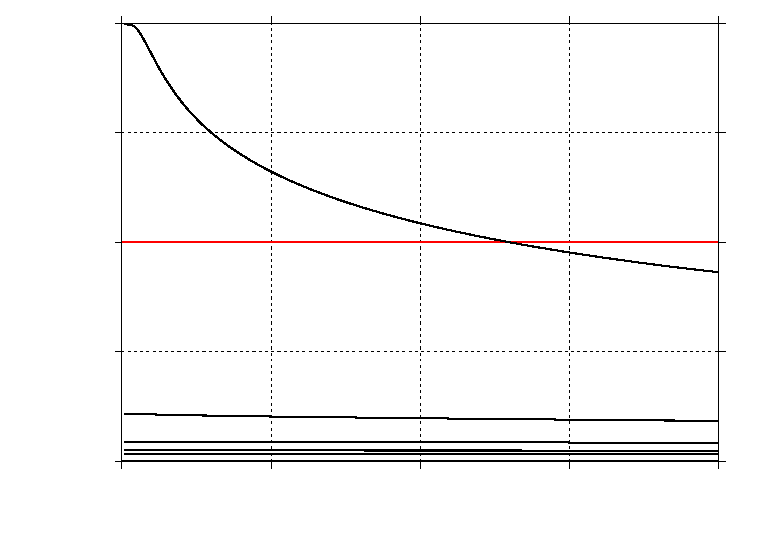
\includegraphics{Figures/TCeigenvalues/TCeigen}}%
    \gplfronttext
  \end{picture}%
\endgroup
  
\caption{In black: The five largest eigenvalues of $L$ plotted as a function of $T$. We see, that the largest eigenvalue intersects 1 (the red line) at one well defined temperature. Parameters: $(n_Ba_{B}^3)^{1/3} = 0.01, (n_Ba_{BF}^3)^{1/3} = 0.1, \frac{m_B}{m_F} = 7/40, \frac{n_F}{n_B^{1/3}} = 0.215$. }
\label{fig.TCeigenvalues}  
\end{center}    
\end{figure}

In figure \ref{fig.TCrB} we see the dependency of $T_c$ on the Bose gas parameter $(n_Ba_B^3)^{1/3}$. We observe a simple monotonic decrease with increasing gas parameter. Physically this can be understood in the following way. When $(n_Ba_B^3)^{1/3}$ is increased for $\frac{n_F}{n_B^{1/3}}$ fixed, the BEC coherence length $k_F\xi = \sqrt{ \frac{\pi}{ 8(n_Ba_B^3)^{1/3} } }\frac{ n_F }{ n_B^{1/3} }$ decreases. The coherence length is the range of the interaction in real space: $\tilde{V}_{\text{ind}} \propto \frac{ \text{e}^{ -\sqrt{2}|x|/\xi } } {|x|}$. Therefore the interaction range is decreased, when we increase $(n_Ba_B^3)^{1/3}$, and so it is physically reasonable, that the critical temperature goes down with increasing $(n_Ba_B^3)^{1/3}$. Notice, that for $(n_Ba_{B}^3)^{1/3} = 0.01$ we recover the critical temperature found in figure \ref{fig.TCeigenvalues}: $T_c \approx 0.130 T_F$. 

\begin{figure} 
\begin{center}  
% GNUPLOT: LaTeX picture with Postscript
\begingroup
  \makeatletter
  \providecommand\color[2][]{%
    \GenericError{(gnuplot) \space\space\space\@spaces}{%
      Package color not loaded in conjunction with
      terminal option `colourtext'%
    }{See the gnuplot documentation for explanation.%
    }{Either use 'blacktext' in gnuplot or load the package
      color.sty in LaTeX.}%
    \renewcommand\color[2][]{}%
  }%
  \providecommand\includegraphics[2][]{%
    \GenericError{(gnuplot) \space\space\space\@spaces}{%
      Package graphicx or graphics not loaded%
    }{See the gnuplot documentation for explanation.%
    }{The gnuplot epslatex terminal needs graphicx.sty or graphics.sty.}%
    \renewcommand\includegraphics[2][]{}%
  }%
  \providecommand\rotatebox[2]{#2}%
  \@ifundefined{ifGPcolor}{%
    \newif\ifGPcolor
    \GPcolorfalse
  }{}%
  \@ifundefined{ifGPblacktext}{%
    \newif\ifGPblacktext
    \GPblacktexttrue
  }{}%
  % define a \g@addto@macro without @ in the name:
  \let\gplgaddtomacro\g@addto@macro
  % define empty templates for all commands taking text:
  \gdef\gplbacktext{}%
  \gdef\gplfronttext{}%
  \makeatother
  \ifGPblacktext
    % no textcolor at all
    \def\colorrgb#1{}%
    \def\colorgray#1{}%
  \else
    % gray or color?
    \ifGPcolor
      \def\colorrgb#1{\color[rgb]{#1}}%
      \def\colorgray#1{\color[gray]{#1}}%
      \expandafter\def\csname LTw\endcsname{\color{white}}%
      \expandafter\def\csname LTb\endcsname{\color{black}}%
      \expandafter\def\csname LTa\endcsname{\color{black}}%
      \expandafter\def\csname LT0\endcsname{\color[rgb]{1,0,0}}%
      \expandafter\def\csname LT1\endcsname{\color[rgb]{0,1,0}}%
      \expandafter\def\csname LT2\endcsname{\color[rgb]{0,0,1}}%
      \expandafter\def\csname LT3\endcsname{\color[rgb]{1,0,1}}%
      \expandafter\def\csname LT4\endcsname{\color[rgb]{0,1,1}}%
      \expandafter\def\csname LT5\endcsname{\color[rgb]{1,1,0}}%
      \expandafter\def\csname LT6\endcsname{\color[rgb]{0,0,0}}%
      \expandafter\def\csname LT7\endcsname{\color[rgb]{1,0.3,0}}%
      \expandafter\def\csname LT8\endcsname{\color[rgb]{0.5,0.5,0.5}}%
    \else
      % gray
      \def\colorrgb#1{\color{black}}%
      \def\colorgray#1{\color[gray]{#1}}%
      \expandafter\def\csname LTw\endcsname{\color{white}}%
      \expandafter\def\csname LTb\endcsname{\color{black}}%
      \expandafter\def\csname LTa\endcsname{\color{black}}%
      \expandafter\def\csname LT0\endcsname{\color{black}}%
      \expandafter\def\csname LT1\endcsname{\color{black}}%
      \expandafter\def\csname LT2\endcsname{\color{black}}%
      \expandafter\def\csname LT3\endcsname{\color{black}}%
      \expandafter\def\csname LT4\endcsname{\color{black}}%
      \expandafter\def\csname LT5\endcsname{\color{black}}%
      \expandafter\def\csname LT6\endcsname{\color{black}}%
      \expandafter\def\csname LT7\endcsname{\color{black}}%
      \expandafter\def\csname LT8\endcsname{\color{black}}%
    \fi
  \fi
    \setlength{\unitlength}{0.0500bp}%
    \ifx\gptboxheight\undefined%
      \newlength{\gptboxheight}%
      \newlength{\gptboxwidth}%
      \newsavebox{\gptboxtext}%
    \fi%
    \setlength{\fboxrule}{0.5pt}%
    \setlength{\fboxsep}{1pt}%
\begin{picture}(7200.00,5040.00)%
    \gplgaddtomacro\gplbacktext{%
      \csname LTb\endcsname%
      \put(946,767){\makebox(0,0)[r]{\strut{}$0$}}%
      \csname LTb\endcsname%
      \put(946,1609){\makebox(0,0)[r]{\strut{}$0.05$}}%
      \csname LTb\endcsname%
      \put(946,2451){\makebox(0,0)[r]{\strut{}$0.1$}}%
      \csname LTb\endcsname%
      \put(946,3292){\makebox(0,0)[r]{\strut{}$0.15$}}%
      \csname LTb\endcsname%
      \put(946,4134){\makebox(0,0)[r]{\strut{}$0.2$}}%
      \csname LTb\endcsname%
      \put(946,4976){\makebox(0,0)[r]{\strut{}$0.25$}}%
      \csname LTb\endcsname%
      \put(1141,484){\makebox(0,0){\strut{}$0.005$}}%
      \csname LTb\endcsname%
      \put(2261,484){\makebox(0,0){\strut{}$0.01$}}%
      \csname LTb\endcsname%
      \put(3381,484){\makebox(0,0){\strut{}$0.015$}}%
      \csname LTb\endcsname%
      \put(4500,484){\makebox(0,0){\strut{}$0.02$}}%
      \csname LTb\endcsname%
      \put(5620,484){\makebox(0,0){\strut{}$0.025$}}%
      \csname LTb\endcsname%
      \put(6740,484){\makebox(0,0){\strut{}$0.03$}}%
    }%
    \gplgaddtomacro\gplfronttext{%
      \csname LTb\endcsname%
      \put(176,2871){\rotatebox{-270}{\makebox(0,0){\strut{}$(n_Ba_B^3)^{1/3}$}}}%
      \put(3940,154){\makebox(0,0){\strut{}$T/T_F$}}%
    }%
    \gplbacktext
    \put(0,0){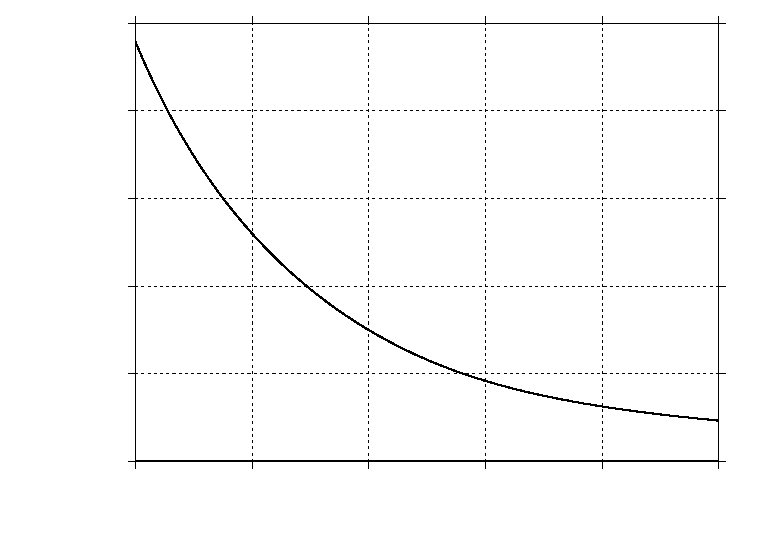
\includegraphics{Figures/TCrB/TCrB}}%
    \gplfronttext
  \end{picture}%
\endgroup
  
\caption{The critical temperatur $T_c$ is plotted as a function of the Bose gas parameter $(n_Ba_B^3)^{1/3}$. We observe a simple monotonic decrease with increasing gas parameter. Other parameters: $(n_Ba_{BF}^3)^{1/3} = 0.1, \frac{m_B}{m_F} = 7/40, \frac{n_F}{n_B^{1/3}} = 0.215$. }  
\label{fig.TCrB}  
\end{center}    
\end{figure}

In figure \ref{fig.TCrBF} we see the dependency of $T_c$ on the Bose-\textit{Fermi} gas parameter $(n_Ba_{BF}^3)^{1/3}$. We observe an increase of $T_c$ with $(n_Ba_{BF}^3)^{1/3}$. This stems from the fact, that a higher value of the Bose-Fermi gas parameter gives a higher interaction strength between the fermions. The system at hand therefore shares one of the key features with the $s$-wave BCS-theory: any nonzero attractive interaction between the fermions leads to a superfluid phase \cite[pp. 156-157]{LandauStatPhys2}. 

\begin{figure} 
\begin{center}  
% GNUPLOT: LaTeX picture with Postscript
\begingroup
  \makeatletter
  \providecommand\color[2][]{%
    \GenericError{(gnuplot) \space\space\space\@spaces}{%
      Package color not loaded in conjunction with
      terminal option `colourtext'%
    }{See the gnuplot documentation for explanation.%
    }{Either use 'blacktext' in gnuplot or load the package
      color.sty in LaTeX.}%
    \renewcommand\color[2][]{}%
  }%
  \providecommand\includegraphics[2][]{%
    \GenericError{(gnuplot) \space\space\space\@spaces}{%
      Package graphicx or graphics not loaded%
    }{See the gnuplot documentation for explanation.%
    }{The gnuplot epslatex terminal needs graphicx.sty or graphics.sty.}%
    \renewcommand\includegraphics[2][]{}%
  }%
  \providecommand\rotatebox[2]{#2}%
  \@ifundefined{ifGPcolor}{%
    \newif\ifGPcolor
    \GPcolorfalse
  }{}%
  \@ifundefined{ifGPblacktext}{%
    \newif\ifGPblacktext
    \GPblacktexttrue
  }{}%
  % define a \g@addto@macro without @ in the name:
  \let\gplgaddtomacro\g@addto@macro
  % define empty templates for all commands taking text:
  \gdef\gplbacktext{}%
  \gdef\gplfronttext{}%
  \makeatother
  \ifGPblacktext
    % no textcolor at all
    \def\colorrgb#1{}%
    \def\colorgray#1{}%
  \else
    % gray or color?
    \ifGPcolor
      \def\colorrgb#1{\color[rgb]{#1}}%
      \def\colorgray#1{\color[gray]{#1}}%
      \expandafter\def\csname LTw\endcsname{\color{white}}%
      \expandafter\def\csname LTb\endcsname{\color{black}}%
      \expandafter\def\csname LTa\endcsname{\color{black}}%
      \expandafter\def\csname LT0\endcsname{\color[rgb]{1,0,0}}%
      \expandafter\def\csname LT1\endcsname{\color[rgb]{0,1,0}}%
      \expandafter\def\csname LT2\endcsname{\color[rgb]{0,0,1}}%
      \expandafter\def\csname LT3\endcsname{\color[rgb]{1,0,1}}%
      \expandafter\def\csname LT4\endcsname{\color[rgb]{0,1,1}}%
      \expandafter\def\csname LT5\endcsname{\color[rgb]{1,1,0}}%
      \expandafter\def\csname LT6\endcsname{\color[rgb]{0,0,0}}%
      \expandafter\def\csname LT7\endcsname{\color[rgb]{1,0.3,0}}%
      \expandafter\def\csname LT8\endcsname{\color[rgb]{0.5,0.5,0.5}}%
    \else
      % gray
      \def\colorrgb#1{\color{black}}%
      \def\colorgray#1{\color[gray]{#1}}%
      \expandafter\def\csname LTw\endcsname{\color{white}}%
      \expandafter\def\csname LTb\endcsname{\color{black}}%
      \expandafter\def\csname LTa\endcsname{\color{black}}%
      \expandafter\def\csname LT0\endcsname{\color{black}}%
      \expandafter\def\csname LT1\endcsname{\color{black}}%
      \expandafter\def\csname LT2\endcsname{\color{black}}%
      \expandafter\def\csname LT3\endcsname{\color{black}}%
      \expandafter\def\csname LT4\endcsname{\color{black}}%
      \expandafter\def\csname LT5\endcsname{\color{black}}%
      \expandafter\def\csname LT6\endcsname{\color{black}}%
      \expandafter\def\csname LT7\endcsname{\color{black}}%
      \expandafter\def\csname LT8\endcsname{\color{black}}%
    \fi
  \fi
    \setlength{\unitlength}{0.0500bp}%
    \ifx\gptboxheight\undefined%
      \newlength{\gptboxheight}%
      \newlength{\gptboxwidth}%
      \newsavebox{\gptboxtext}%
    \fi%
    \setlength{\fboxrule}{0.5pt}%
    \setlength{\fboxsep}{1pt}%
\begin{picture}(7200.00,5040.00)%
    \gplgaddtomacro\gplbacktext{%
      \csname LTb\endcsname%
      \put(946,767){\makebox(0,0)[r]{\strut{}$0$}}%
      \csname LTb\endcsname%
      \put(946,1415){\makebox(0,0)[r]{\strut{}$0.02$}}%
      \csname LTb\endcsname%
      \put(946,2062){\makebox(0,0)[r]{\strut{}$0.04$}}%
      \csname LTb\endcsname%
      \put(946,2710){\makebox(0,0)[r]{\strut{}$0.06$}}%
      \csname LTb\endcsname%
      \put(946,3357){\makebox(0,0)[r]{\strut{}$0.08$}}%
      \csname LTb\endcsname%
      \put(946,4005){\makebox(0,0)[r]{\strut{}$0.1$}}%
      \csname LTb\endcsname%
      \put(946,4652){\makebox(0,0)[r]{\strut{}$0.12$}}%
      \csname LTb\endcsname%
      \put(1141,484){\makebox(0,0){\strut{}$0$}}%
      \csname LTb\endcsname%
      \put(2261,484){\makebox(0,0){\strut{}$0.02$}}%
      \csname LTb\endcsname%
      \put(3381,484){\makebox(0,0){\strut{}$0.04$}}%
      \csname LTb\endcsname%
      \put(4500,484){\makebox(0,0){\strut{}$0.06$}}%
      \csname LTb\endcsname%
      \put(5620,484){\makebox(0,0){\strut{}$0.08$}}%
      \csname LTb\endcsname%
      \put(6740,484){\makebox(0,0){\strut{}$0.1$}}%
    }%
    \gplgaddtomacro\gplfronttext{%
      \csname LTb\endcsname%
      \put(176,2871){\rotatebox{-270}{\makebox(0,0){\strut{}$T_c/T_F$}}}%
      \put(3940,154){\makebox(0,0){\strut{}$(n_Ba_{BF}^3)^{1/3}$}}%
    }%
    \gplbacktext
    \put(0,0){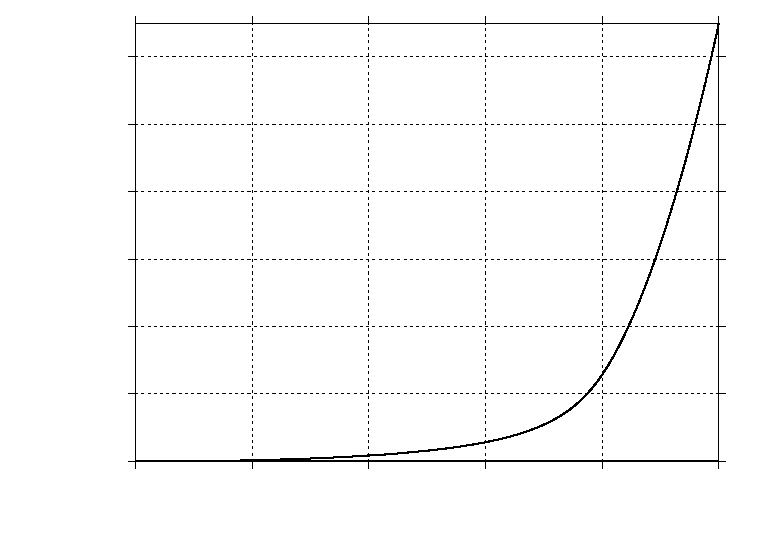
\includegraphics{Figures/TCrBF2/TCrBF}}%
    \gplfronttext
  \end{picture}%
\endgroup
  
\caption{The critical temperatur $T_c$ is plotted as a function of the Bose-Fermi gas parameter $(n_Ba_{BF}^3)^{1/3}$. We see, that for every nonzero induced interaction, there is a superfluid phase for $T\to 0$. Other parameters: $(n_Ba_{B}^3)^{1/3} = 0.01, \frac{m_B}{m_F} = 7/40, \frac{n_F}{n_B^{1/3}} = 0.215$. }  
\label{fig.TCrBF}  
\end{center}    
\end{figure}





\addtocontents{toc}{\vspace{2em}} % Add a gap in the Contents, for aesthetics

\backmatter

%----------------------------------------------------------------------------------------
%	BIBLIOGRAPHY
%----------------------------------------------------------------------------------------

\label{Bibliography}

%\bibliographystyle{unsrtnat} % Use the "unsrtnat" BibTeX style for formatting the Bibliography
%\bibliography{Bibliography} % The references (bibliography) information are stored in the file named "Bibliography.bib"
\printbibliography
\chead{}
\lhead{\emph{Bibliography}} % Change the page header to say "Bibliography"
 



\end{document}  